\documentclass[letterpaper,12pt,peerreviewca,draftcls]{IEEEtran}
\usepackage{csm16}
\usepackage[margin=1in]{geometry}
\usepackage[nolists,nomarkers,tablesfirst]{endfloat} % put figures at end
\usepackage{amsmath} % for \eqref
\usepackage{mathtools}
% added for CSMAG only
\usepackage{url}
\usepackage{graphicx,xcolor}
\usepackage{verbatim}% http://ctan.org/pkg/verbatim
\makeatletter
\newcommand{\verbatimfont}[1]{\def\verbatim@font{#1}}%
\makeatother
\verbatimfont{\ttfamily\small}
\newcommand{\XX}[1]{{\bf \color{orange}{ XX #1 XX}}}
\newcommand{\rr}[1]{{\bf \color{blue}{#1}}}
%\usepackage{subfigure} 


%
\usepackage[left,pagewise]{lineno} 
\usepackage[english]{babel} 
%\usepackage{blindtext}
% added for CSMAG only

\usepackage{etex}
\usepackage[authormarkuptext=name,addedmarkup=bf,authormarkupposition=left]{changes}

\definecolor{DarkRed}{rgb}{0.75,0,0}
\definecolor{DarkGreen}{rgb}{0,0.5,0}
\definecolor{DarkBlue}{rgb}{0,0,0.5}
\definecolor{DarkPurple}{rgb}{0.5,0,0.5}
\definecolor{LightGrey}{rgb}{0.9,0.9,0.9}

\definechangesauthor[name={M.~L.}, color={blue}]{ml}
\definechangesauthor[name={G.~C.}, color={DarkGreen}]{gc}
\definechangesauthor[name={S.~L.}, color={green}]{sl}
\definechangesauthor[name={B.~C.}, color={red}]{bc}
\definechangesauthor[name={J.~H.}, color={DarkPurple}]{jh}
                              \newcommand{\mX}[1]{\added[id=ml,remark={}]{#1}}
\newcommand{\gX}[1]{\added[id=gc,remark={}]{#1}}
\newcommand{\sX}[1]{\added[id=sl,remark={}]{#1}}
\newcommand{\bX}[1]{\added[id=bc,remark={}]{#1}}
\newcommand{\jX}[1]{\added[id=jh,remark={}]{#1}}

%
\usepackage[left,pagewise]{lineno} 
% added for CSMAG only

\usepackage{amssymb,amsmath,bm,booktabs,amsthm}
\usepackage[sort,compress]{cite}
%\usepackage{algorithm,algcompatible}
\usepackage{algorithm}
\usepackage{algorithmic}
%\usepackage{algpseudocode}
%for making comments in algorithm
%\renewcommand{\COMMENT}[2][.5\linewidth]{%
%	\leavevmode\hfill\makebox[#1][l]{//~#2}}

\usepackage{subfig}
%\usepackage{subcaption}
\usepackage{eqparbox}
\renewcommand\algorithmiccomment[1]{%
  \hfill\#\ \eqparbox{COMMENT}{#1}%
}

\usepackage{etoolbox}  % patch def of algorithmic environment
\makeatletter
\patchcmd{\algorithmic}{\addtolength{\ALC@tlm}{\leftmargin} }{\addtolength{\ALC@tlm}{\leftmargin}}{}{}
\makeatother
 \usepackage{tikz}
 \usepackage{tikz-qtree}
 \usetikzlibrary{decorations.pathreplacing,calc}
 \usetikzlibrary{arrows}
 \usetikzlibrary{positioning}
 \usetikzlibrary{matrix}

 % tikz macros for scaling etc. 
 \newcommand{\yslant}{0}
 \newcommand{\xslant}{0}
 \newcommand{\diagscale}{0.35}
 \newcommand{\diagtexttop}{0.51}
 \newcommand{\diagtext}{0.45}

 
 \newcommand*{\AddNote}[4]{%
     \begin{tikzpicture}[overlay, remember picture]
         \draw [decoration={brace,amplitude=0.5em},decorate,ultra thick,red]
             ($(#3)!(#1.north)!($(#3)-(0,1)$)$) --  
             ($(#3)!(#2.south)!($(#3)-(0,1)$)$)
                 node [align=center, text width=2.5cm, pos=0.5, anchor=west] {#4};
     \end{tikzpicture}
 }%
 
% \usepackage{wrapfig}
 \usetikzlibrary{automata}
 \usetikzlibrary{arrows,snakes,backgrounds}
 \tikzstyle{ball} = [circle,shading=ball, ball color=black!80!white,
     minimum size=1cm]
 \tikzstyle{ball2} = [circle,shading=ball, ball color=red!80!white,
     minimum size=1cm]
 \tikzstyle{ball3} = [circle,shading=ball, ball color=blue!80!white,
     minimum size=1cm]
 \tikzstyle{ball4} = [circle,shading=ball, ball color=green!100!white,
     minimum size=1cm]
 \tikzstyle{ball5} = [circle,shading=ball, ball color=purple!80!white,
     minimum size=1cm]       
     
%\usepackage[hidelinks,pdftex]{hyperref}
\usepackage[pdftex, plainpages = false, colorlinks=true, linkcolor=black, citecolor = green!50!blue, urlcolor = blue, filecolor=black, pagebackref=false, hypertexnames=false,  pdfpagelabels ]{hyperref}

\usepackage[capitalise]{cleveref}
\crefname{equation}{}{}

\usepackage{comment}
\renewcommand{\algorithmicrequire}{\textbf{Input:}}
\renewcommand{\algorithmicensure}{\textbf{Output:}}
%\sethlcolor{LightGrey}

\usepackage[normalem]{ulem}

\newcounter{JPH}
%\newtheorem{sidebartheorem}{\textit{Theorem}~S\!\!}[JPH]

\newcounter{sidebartheorem}
%\renewcommand{\thesidebartheorem}{\Alph{JPH}\thesidebartheore}
\newenvironment{sidebartheorem}[1][]{\refstepcounter{sidebartheorem}\par\medskip \textit{Theorem~S\thesidebartheorem} #1:\rmfamily}{\medskip}
\newcommand{\sidebarref}[1]{S\ref{#1}}


\usepackage[nolists,tablesfirst,nomarkers]{endfloat}
 
\title{Evolving Gaussian Processes and Kernel Observers for Learning and Control in Spatiotemporally Varying Domains\\\Large with applications in agriculture, weather monitoring, and fluid dynamics}
\author{Joshua E. Whitman, Harshal Maske, Hassan A. Kingravi, Girish Chowdhary, \\ POC email: girishc@illinois.edu}

\newif\ifPDF \ifx\pdfoutput\undefined\PDFfalse \else\ifnum\pdfoutput > 0\PDFtrue \else\PDFfalse \fi \fi
\ifPDF 
%\usepackage[pdftex, plainpages = false, colorlinks=true, linkcolor=black, citecolor = green!50!blue, urlcolor = blue, filecolor=black, pagebackref=false, hypertexnames=false,  pdfpagelabels ]{hyperref}
\fi
\graphicspath{{figures/}}
\newif\ifPDF \ifx\pdfoutput\undefined \PDFfalse \else \ifnum \pdfoutput > 0 \PDFtrue \else\PDFfalse \fi \fi

%\newcommand{\qed}{\nobreak \ifvmode \relax \else
%      \ifdim\lastskip<1.5em \hskip-\lastskip
%      \hskip1.5em plus0em minus0.05em \fi \nobreak
%      \vrule height0.25em width0.5em depth0.25em\fi}

%\usepackage[usenames]{color}
\usepackage[normalem]{ulem}
\newcommand{\gXX}[1]{\color{red} XX #1 XX \color{black}}
\newcommand{\hXX}[1]{\color{green} XX #1 XX \color{black}}
\newcommand{\gcmargin}[2]{{\color{red}#1}\marginpar{\color{red}\tiny\raggedright \bf [GC] #2}}
\newcommand{\hkmargin}[2]{{\color{red}#1}\marginpar{\color{green}\tiny\raggedright \bf [HK] #2}}
\newcommand{\gsec}[1]{\fcolorbox{DarkRed}{DarkRed}{\parbox{3in}{\raggedright \color{green} #1 }}}
\newcommand{\gsout}[2]{{\sout{#1}}{{\gXX{#2}}}}



\newcommand{\bea}{\begin{eqnarray}}
\newcommand{\eea}{\end{eqnarray}}
\newcommand{\be}{\begin{equation}}
\newcommand{\ee}{\end{equation}}
\newcommand{\bi}{\begin{itemize}}
\newcommand{\ei}{\end{itemize}}
%\newcommand{\XX}{{\bf XX}} %\XX
\newcommand{\nn}{{\nonumber}}
\newcommand{\motiv}{{\bf Why, How, Who cares?}}
\newcommand{\mean}{{\bf E}}
\newcommand{\meanw}{{\bf E}_w}
\newcommand{\boldp}{\bf P}
\newcommand{\boldsp}{\bf p}
\newcommand{\cov}{{\bf \Sigma}}
\newcommand{\maxmu}{{\max_\mu}}
\newcommand{\maxtmu}{{\max_{\tilde{\mu}}}}
\newcommand{\tmu}{\tilde{\mu}}
\newcommand{\hmu}{\hat{\mu}}
\newcommand{\mui}{\mu^i}
\newcommand{\mukki}{\mu^i_{k|k}}
\newcommand{\mukkj}{\mu^j_{k|k}}
\newcommand{\mukpki}{\mu^i_{k+1|k}}
\newcommand{\mukpkpi}{\mu^i_{k+1|k+1}}
\newcommand{\x}{\mathcal{X}}
\newcommand{\iso}{\boldsymbol{1_s}}
\newcommand{\dd}{\boldsymbol{1_{di}}}

\newcommand{\tPi}{\tilde{\Pi}}
\newcommand{\tpi}{\tilde{\pi}}
\newcommand{\tLambda}{\tilde{\Lambda}}
\newcommand{\hatxk}{\hat{x}_{k|k}}
\newcommand{\hatxkk}{\hat{x}_{k+1|k+1}}
\newcommand{\hatxkki}{\hat{x}_{k+1|k+1}^i}
\newcommand{\hatxki}{\hat{x}_{k|k}^i}
\newcommand{\Pk}{P_{k|k}}
\newcommand{\Pkk}{P_{k+1|k+1}}
\newcommand{\Pki}{P_{k|k}^i}
\newcommand{\Pkki}{P_{k+1|k+1}^i}

\newcommand{\matlabpathrmmmeas}{C:/MATLAB7/work/UMC/RobustMM/UAV_TrackingMM/MeasurementUpdate}
\newcommand{\matlabpathrmmd}{C:/MATLAB7/work/UMC/RobustMM/UAV_TrackingMM/Version1}
\newcommand{\matlabpathrmmvv}{C:/MATLAB7/work/UMC/RobustMM/UAV_TrackingMM/Version4}
\newcommand{\matlabpathrmm}{C:/MATLAB7/work/UMC/RobustMM/UAV_TrackingMM/Version3}
\newcommand{\matlabpathrmmtwod}{C:/MATLAB7/work/UMC/RobustMM/UAV_TrackingMM/Version3/Figs/}
\newcommand{\matlabpathrmmprob}{C:/MATLAB7/work/UMC/RobustMM/ProblemViz}
\newcommand{\robmmpath}{C:/Documents and Settings/Luca F. Bertuccelli/My Documents/Research/UncertainMarkovChain/RobustMM/}
\usepackage{multirow}
\newtheorem{theorem}{Theorem}%[section]
\newtheorem{definition}{Definition}
\newtheorem{proposition}{Proposition}
\newtheorem{corollary}{Corollary}
\newtheorem{lemma}{Lemma}
\newtheorem{remark}{Remark}

% matrix
\newcommand{\bbm}{\begin{bmatrix}}
\newcommand{\ebm}{\end{bmatrix}}

% itemize
%\newcommand{\bi}{\begin{itemize}}
%\newcommand{\ei}{\end{itemize}}

% enumerate
\newcommand{\ben}{\begin{enumerate}}
\newcommand{\een}{\end{enumerate}}

% equationarray
%\newcommand{\bea}{\begin{eqnarray}}
%\newcommand{\eea}{\end{eqnarray}}

% equation
%\newcommand{\be}{\begin{equation}}
%\newcommand{\ee}{\end{equation}}
\newcommand{\bes}{\begin{eqnarray*}}
\newcommand{\ees}{\end{eqnarray*}}

% indent
\newcommand{\nid}{\noindent}

% figure
\newcommand{\bfig}{\begin{figure}}
\newcommand{\efig}{\end{figure}}

% center
\newcommand{\bc}{\begin{center}}
\newcommand{\ec}{\end{center}}

% bullet
\newcommand{\nb}{\noindent $\bullet$\hspace{1.5mm}}

% ignore
\newcommand{\ignore}[1]{}

% spaces
\newcommand{\hs}[1]{\hspace{#1mm}}
\newcommand{\vs}[1]{\vspace{#1mm}}

% lists / enumerations
\newcommand{\beni}[2]
{\begin{enumerate}\setlength{\itemsep}{#1mm}\setlength{\parskip}{#2mm}}

\newcommand{\bii}[2]
{\begin{itemize}\setlength{\itemsep}{#1mm}\setlength{\parskip}{#2mm}}

% comments












% % % % % % % % % % % % % % % % % % % % % % % % % % % % % % % % % % % % % % % % % % % % % % % % % % % % % % % %
% % % % % % % % % % % % % % % % % % % % % % % % % % % % % % % % % % % % % % % % % % % % % % % % % % % % % % % % % %
\newcommand{\al}{\alpha}
%\newcommand{\be}{\beta}
\newcommand{\e}{\epsilon}
\newcommand{\la}{\lambda}
\newcommand{\s}{\sigma}
\newcommand{\p}{\partial}
\newcommand{\R}{\mathbb{R}}
\newcommand{\E}{\mathbb{E}}
\newcommand{\tr}{\mathrm{tr}}
\newcommand{\LI}{\mathcal{L}}
\newcommand{\Co}{\mathcal{C}}
\newcommand{\C}{\mathbb{C}}
\newcommand{\F}{\mathcal{F}}
\newcommand{\W}{\mathcal{W}}
\newcommand{\K}{\mathbf{K}}
\newcommand{\Z}{\mathbf{Z}}
\newcommand{\w}{\mathbf{w}}
\newcommand{\Be}{\mathbf{\beta}}
\newcommand{\y}{\mathbf{y}}
\DeclareMathOperator{\GP}{GP}
\newcommand{\BV}{\mathcal{BV}}
\newcommand{\Hi}{\mathcal{H}}
\newcommand{\No}{\mathcal{N}}
\newcommand{\V}{\mathbb V}
\newcommand{\La}{\mathcal{L}}


%\def\i{\infty}
\def\l{\langle}
\def\v{\varphi}
\def\r{\rangle}
\def\m{\mathbf}
\def\H{\mathcal{H}}
\def\O{\mathcal{O}}
\def\P{\mathbb{P}}
\def\Ny{ Nystr\"{o}m }

% define paper-specific macros

% Hilbert space/basis function macros
\newcommand{\bfunc}{\phi}
\newcommand{\bvect}{\Phi}
\newcommand{\uncertainty}{\Delta}
\newcommand{\weight}{w}
\newcommand{\estweight}{\widehat{w}}
\newcommand{\idweight}{{W^{*}}}
\newcommand{\fweight}{\mathbf{W^*}}
\newcommand{\fspace}{\mathcal{H}}
\newcommand{\dspace}{\mathcal{H}^*}
\newcommand{\fmap}{\psi}
\newcommand{\fdim}{M}
\newcommand{\fevec}{\mathbf{\xi}}
\newcommand{\fefunc}{\mathbf{\phi}}
\newcommand{\feval}{\mathbf{\lambda}}
\newcommand{\fsol}{\mathbf{\varphi}}
\newcommand{\fvect}{\Psi}
\newcommand{\proj}{\gamma}
\newcommand{\sysop}{\mathcal{A}}
\newcommand{\estsysop}{\widehat{A}}
\newcommand{\controlop}{\mathcal{B}}
\newcommand{\measop}{\mathcal{K}}
\newcommand{\estmeasop}{K}
\newcommand{\sloc}{S}
\newcommand{\centers}{C}
\newcommand{\centerscontrol}{D}
\newcommand{\weights}{{w}}

% dynamical system macros
\newcommand{\state}{x}
\newcommand{\astate}{z}
\newcommand{\aastate}{z}%in time varying this should be \bar {z}
\newcommand{\statesize}{n_s}
\newcommand{\isize}{n}
\newcommand{\sdomain}{D_x}
\newcommand{\tdomain}{D_{\tau}}
\newcommand{\tvarsig}{\tau}
\newcommand{\tsize}{m}
\newcommand{\sdefunc}{F}
\newcommand{\sysfunc}{f}
\newcommand{\control}{\delta}
\newcommand{\cdomain}{D_{\delta}}
\newcommand{\csize}{l}
\newcommand{\pcontrol}{\nu}
\newcommand{\asysfunc}{\hat{f}}
\newcommand{\terror}{e}
\newcommand{\reference}{r}
\newcommand{\rstate}{x_{rm}}
\newcommand{\lyap}{V}
\newcommand{\nneval}{\varsigma}
\newcommand{\adElement}{\nu_{ad}}
\newcommand{\measnoise}{\zeta}
\newcommand{\processnoise}{\eta}


% Gaussian process macros
\newcommand{\kernel}{k}
\newcommand{\kernelvec}{\mathbf{k}}
\newcommand{\estKernel}{\hat{k}}
\newcommand{\evalKernel}{k^*}
\newcommand{\kernelM}{K}
\newcommand{\estKernelM}{\hat{K}}
\newcommand{\meas}{y}
\newcommand{\estmeas}{\widehat{y}}
\newcommand{\imean}{m}
\newcommand{\pVar}{\Sigma}
\newcommand{\Covar}{C}
\newcommand{\estMean}{\hat{m}}
\newcommand{\estPVar}{\hat{\Sigma}}
\newcommand{\switchiMean}{m^{\sigma}}
\newcommand{\switchMean}{\hat{m}^{\sigma}}
\newcommand{\errMean}{\epsilon_m}
\newcommand{\switchErrMean}{\epsilon_m^{\sigma}}
\newcommand{\bstack}{Z}
\newcommand{\zstackT}{Z_\tau}
\newcommand{\Tdisc}{\tau}
\newcommand{\etasup}{\eta_{\mathrm{sup}}}
\newcommand{\stateideal}{\bar{x}}
\newcommand{\nuavail}{\nu_{\mathrm{avail}}}
% miscellaneous macros
\newcommand{\switch}{\sigma}
\newcommand{\Index}{\mathcal{I}}

% integral operator and density macros
\newcommand{\idealP}{\ensuremath{{p}}}
\newcommand{\idealK}{\ensuremath{{\m{K}}}}
\newcommand{\eval}{\la}
\newcommand{\efunc}{\ensuremath{\phi}}
\newcommand{\empEfunc}{\ensuremath{\widehat \phi}}
\newcommand{\empEval}{\ensuremath{\widehat \la}}
\newcommand{\delP}{\ensuremath{{p_{\delta}}}}
\newcommand{\delEmpP}{\ensuremath{\widehat p_{\delta}}}
\newcommand{\empP}{\ensuremath{\widehat p}}
\newcommand{\shP}{\ensuremath{\widetilde p}}
\newcommand{\kMax}{\ensuremath{\kappa}}
\newcommand{\probMeas}{\ensuremath{\mu}}

% matrix and vector macros
\newcommand{\empK}{\ensuremath{K}}
\newcommand{\shK}{\ensuremath{\widetilde K}}
\newcommand{\idealshK}{\ensuremath{\widetilde{\m{K}}}}
\newcommand{\shG}{\ensuremath{\widetilde G}}
\newcommand{\CK}{K^{\shCent}}
\newcommand{\quaK}{\ensuremath{\bar{K}}}
\newcommand{\quaC}{\ensuremath{\oline{\mathcal{C}}}}
\newcommand{\evecs}{\ensuremath{U}}
\newcommand{\evalM}{\ensuremath{\Lambda}}
\newcommand{\extrap}{\ensuremath{E}}
\newcommand{\normChoice}{\xi}

\newcommand{\Dist}{\mathcal{D}}
\newcommand{\DDist}{\mathbb{D}}

% dataset and reduced set macros 
\newcommand{\dom}{\Omega}
\newcommand{\domI}{\Omega_I}
\newcommand{\domO}{\Omega_O}
\newcommand{\sampSet}{\mathcal{X}}
\newcommand{\sampSetOther}{\mathcal{Y}}
\newcommand{\sampSetClass}{\mathcal{D}}
\newcommand{\sampSetLong}{\{x_1, \dots, x_{\nsamp}\}}
\newcommand{\sampSetClassLong}{\{(x_1,y_1), \dots, (x_{\nsamp},y_{\nsamp})\}}
\newcommand{\sampSetShort}{\{\astate_i\}_{1}^{\Tdisc}}
\newcommand{\sampSetClassShort}{\{(x_i,y_i)\}_{1}^{\nsamp}}
\newcommand{\card}[1]{\left|{#1}\right|}
\newcommand{\cent}{c}
\newcommand{\nsamp}{N}
\newcommand{\ncent}{M}
\newcommand{\dtime}{\tau}
\newcommand{\ntrain}{n_{t}}
\newcommand{\ntest}{n_{te}}
\newcommand{\neigs}{r}
\newcommand{\shCent}{\mathcal{C}}
\newcommand{\shCentLong}{\{c_1,\dots,c_{\ncent}\}}
\newcommand{\weightSet}{\W}
\newcommand{\weightSetLong}{\{w_1, \dots, w_{\ncent}\}}
\newcommand{\recSet}{\delta X}
\newcommand{\shSet}{S}
\newcommand{\shrad}{\varepsilon}

\newcommand{\G}{\mathcal{G}}
\newcommand{\X}{\mathcal{X}}

\newcommand{\statesizea}{n_1}
\newcommand{\statesizeb}{n_2}
%\newcommand{\statesize2}{n_2}

\DeclareMathOperator*{\argmin}{arg\,min}
\DeclareMathOperator{\HS}{HS}

\newcommand{\eqlabel}[1]{\label{eq:#1}}
\newcommand{\EQref}[1]{Eq.~(\ref{eq:#1})}
\renewcommand{\eqref}[1]{(\ref{eq:#1})}

\newcommand{\EGP}{\text{EGP}}
\newcommand{\swindex}{j}
\newcommand{\RKHS}{RKHS~}



\newcommand{\sgn}{\mathrm{sgn}}
\newcommand{\refm}{\mathrm{ref}}
\newcommand{\des}{\mathrm{des}}
\newcommand{\Sa}{\mathcal{S}}
\newcommand{\A}{\mathcal{A}}
\newcommand{\T}{\mathcal{T}}



% dynamical system macros

\newcommand{\controlfunc}{b}

\newcommand{\acontrolfunc}{\hat{b}}

% Gaussian process macros





\newcommand{\fow}{\Upsilon}
\newcommand{\FoW}{FOW~}

\DeclareMathOperator{\vol}{vol}

% % hybrid systems
\newcommand{\cont}{x}
\newcommand{\discrete}{x^+}

\DeclareMathOperator{\Dir}{Dir}
\DeclareMathOperator{\BP}{BP}
\DeclareMathOperator{\BeP}{BeP}


%from Hassan


%\newcommand{\DiscP}{\mathbb{D}}
\newcommand{\parms}{\Theta}
\newcommand{\MN}{\mathcal{MN}}
\newcommand{\err}{\mathbf{e}}
\newcommand{\errCov}{\mathbf{\Sigma}}
\newcommand{\zero}{\mathbf{0}}
\newcommand{\pastData}{\mathcal{W}}
\newcommand{\pastDataL}{\bar{\mathcal{W}}}
\newcommand{\pastBoth}{\mathcal{D}}
\newcommand{\pastErr}{\mathbf{E}}
\newcommand{\postWish}{\mathbf{S}_{w\bar{w}}}
\newcommand{\postWishLL}{\bar{\mathbf{S}}_{\bar{w}\bar{w}}}
\newcommand{\postWishLLI}{\bar{\mathbf{S}}^{-\swindex}_{\bar{w}\bar{w}}}
\newcommand{\postWishL}{\mathbf{S}_{\bar{w}\bar{w}}}
\newcommand{\postWishS}{\mathbf{S}_{w|\bar{w}}}



\def\i{\infty}
\def\l{\langle}
\def\v{\varphi}
\def\r{\rangle}
\def\m{\mathbf}
\def\H{\mathcal{H}}
\def\O{\mathcal{O}}
\def\P{\mathbb{P}}
\def\Na{\mathbb{N}}
\def\Ny{ Nystr\"{o}m }

% define paper-specific macros

% Hilbert space/basis function macros

\newcommand{\nsysop}{\mathcal{G}}

% Gaussian process macros

% dataset and reduced set macros 


% E-GP specific macros
\newcommand{\egpFunc}{f}
\newcommand{\egpDyn}{g}

\newcommand{\EGPFspace}{\mathbb{H}}
\newcommand{\EGPSample}{\mathbb{F}}
\newcommand{\EGPFspaces}{\coprod_{j=1}^{\infty}\fspace^j}



% VV Stuff
\newcommand{\Kr}{\m{K}}
\newcommand{\f}{\m{f}}
%\newcommand{\I}{\m{I}}


\DeclareMathOperator{\Var}{Var}
\DeclareMathOperator{\grad}{grad}
\DeclareMathOperator{\diag}{diag}
\DeclareMathOperator{\MMD}{MMD}
\DeclareMathOperator{\divergence}{div}
\DeclareMathOperator{\Span}{span}
%\DeclareMathOperator{\span}{span}
\DeclareMathOperator{\Rank}{rank}
\DeclareMathOperator{\Pro}{\mathbb{P}}
\DeclareMathOperator*{\argmax}{arg\,max}

%\newcommand{\statesize2}{n_2}


\DeclareMathOperator{\DiscP}{Disc}
\DeclareMathOperator{\IW}{IW}
\DeclareMathOperator{\Tr}{Tr}


%\renewcommand{\eqref}[1]{(\ref{eq:#1})}

\newcommand{\NMBRL}{N-MBRL}


% new macros
\newcommand{\dimI}{\ensuremath{D}}
\newcommand{\dimO}{\ensuremath{d}}
\newcommand{\dimP}{\ensuremath{P}}
\newcommand{\sO}{\mathcal{S}}
\newcommand{\risk}{\mathop{\mathbf{R}}}
\newcommand{\empRisk}{\mathop{\widehat{\mathbf{R}}}}
\newcommand{\radCom}{{\mathcal{R}}}
\newcommand{\funcClass}[1]{\mathcal{F}_{#1}}
\newcommand{\empFuncClass}[1]{\widehat{\mathcal{F}}_{#1}}
\newcommand{\oweights}{\ensuremath{\alpha}}
\newcommand{\loss}{\ell}

% newer macros
\newcommand{\Obs}{\mathcal{O}}
\newcommand{\otime}{L}
\newcommand{\JorMul}{O}
\newcommand{\Tset}{\Upsilon}
\newcommand{\measmat}{\Phi}
\newcommand{\enrgy}{\gamma}
\newcommand{\eenrgy}{\lambda}
\newcommand{\blockmat}{\boldsymbol\Phi}
\newcommand{\modker}{\widehat\kernel}
\newcommand{\centker}{\widetilde\kernel}
\newcommand{\Dim}{D}
\newcommand{\Ind}{\mathcal{I}}
\newcommand{\LaVec}{\boldsymbol{\la}}
\newcommand{\LaMat}{\boldsymbol{\Lambda}}
\newcommand{\JorP}{P}
\newcommand{\JorLa}{\Lambda}
\newcommand{\empKDiag}{\mathbf{K}^D}
%\newcommand{\empKMod}{\widetilde{\empK}} %repeated twice
\newcommand{\empKBlock}{\widehat{\mathbf{K}}} % now catempK
%\newcommand{\ABlock}{\widehat{\mathbf{A}}} %now defined as \catdualopC
\newcommand{\Coh}{\mathcal{C}}

% feature map macros
\newcommand{\fspaceC}{\ensuremath{\mathcal{H}^{\mathcal{C}}}}
\newcommand{\fspaceD}{\ensuremath{\widetilde{\fspace}}}
\newcommand{\functionSet}{\mathcal{J}}
\newcommand{\AtomsControl}{\mathcal{F}_{\centerscontrol}}
\newcommand{\fspaceApprox}{\widehat{\fspace}}
\newcommand{\fsubspaceApprox}[1]{\fspaceApprox_{#1}}
\newcommand{\fmapApprox}{\widehat{\fmap}}
\newcommand{\fbasis}{\psi}
\newcommand{\fspaceEl}{f}
\newcommand{\fspaceApproxEl}{\widehat{\fspaceEl}}
\newcommand{\obsMat}{\empK}
\newcommand{\randFreq}{\omega}
\newcommand{\randMat}{V}
\newcommand{\obsMatRow}{\widehat{\Psi}}
\newcommand{\Kiprod}[2]{\langle \fmap(#1),\fmap(#2) \rangle_{\fspace}}
\newcommand{\Atoms}{\mathcal{F}^{\shCent}}

% controls specific stuff
\newcommand{\weightmap}{\ensuremath{\mathcal{W}}}
\newcommand{\weightmapI}{\ensuremath{\mathcal{W}^{-1}}}
\newcommand{\weightmapC}{\ensuremath{\acute{\mathcal{W}}}}
\newcommand{\weightmapCI}{\ensuremath{\acute{\mathcal{W}}^{-1}}}
\newcommand{\data}{X}
\newcommand{\ncontrol}{\ell'}
\newcommand{\weightc}{\acute{\weight}}
\newcommand{\empKD}{\empK_{\centerscontrol}}
\newcommand{\empKCD}{\empK_{\centers\centerscontrol}}
\newcommand{\ControlMat}{\Psi}
\newcommand{\controlCent}{\mathcal{D}}
\newcommand{\controlCentLong}{\{d_1,\dots,d_{\ncontrol}\}}
\newcommand{\cbasis}{\widetilde{\psi}}

% minimal polynomial and measurement map etc
\newcommand{\charpoly}{\pi}
\newcommand{\minpoly}{\alpha}
\newcommand{\minpolyv}{\xi}
\newcommand{\geomMult}[1]{\gamma_{#1}}
\newcommand{\algMult}[1]{\mu_{#1}}
\newcommand{\genMult}[1]{\nu_{#1}}
\newcommand{\rank}{r}
\newcommand{\nevals}{r}
\newcommand{\linvec}{v}
\newcommand{\polycoeff}{a}
\newcommand{\acycdeg}{m}
\newcommand{\minmeas}{\ell}
\newcommand{\linspace}{\mathcal{V}}
\newcommand{\linspaceout}{\mathcal{U}}
\newcommand{\subspace}{\linspace_{\mathcal{S}}}
\newcommand{\measmap}{\widetilde{\empK}}
\newcommand{\premeasmap}{\mathring{\empK}}
\newcommand{\measmapsum}{\check{\empK}}
\newcommand{\mmapInd}[1]{\mathcal{J}^{({#1})}}
\newcommand{\restrict}[2]{{#1}_{|#2}}
\newcommand{\fsubspaceC}[1]{\fspaceApprox_{#1}}
\newcommand{\initcondf}{\widetilde{f}}
\newcommand{\initcond}{\weight_0}
\newcommand{\sysopC}{\sysop_{\shCent}}
\newcommand{\sysopApprox}{\widehat{\sysop}}
\newcommand{\dualop}{A}
\newcommand{\dualopC}{A_{\shCent}}
\newcommand{\dualopApprox}{\widehat{\dualop}}
\newcommand{\empKShadFull}{\mathbf{\empK}}

\newcommand{\sampind}{i}
\newcommand{\centind}{j}
\newcommand{\setind}{\iota}

% kernel observer transition macros
\newcommand{\tindex}{\tau}
\newcommand{\ftime}{T}
\newcommand{\orbit}{\boldsymbol{\Theta}}
\newcommand{\banachspace}{\mathcal{B}}
\newcommand{\banachop}{\mathcal{L}}
\newcommand{\banachfunc}{u}
\newcommand{\rands}{\varsigma}

\DeclareMathOperator{\dims}{dim}
\DeclareMathOperator{\degs}{deg}
\DeclareMathOperator{\Ker}{Ker}

%Borrowed from CDC
\newcommand{\evalvec}{\boldsymbol{\eval}}
% supplementary macros
\newcommand{\transempK}{\breve{\empK}}
\newcommand{\catempK}{\widehat{\mathbf{K}}}
\newcommand{\catdualopC}{\widehat{\mathbf{A}}}
\newcommand{\catJorP}{\boldsymbol{\JorP}}
\newcommand{\catJorLa}{\boldsymbol{\JorLa}}
\newcommand{\estdualopC}{\widehat{A}_{\shCent}}
\newcommand{\estcontrolop}{\widehat{B}}

% decomposition macros
\newcommand{\Fmap}{\Psi}
%\newcommand{\LaMat}{\boldsymbol{\Lambda}}
%\newcommand{\JorP}{P}
%\newcommand{\JorLa}{\Lambda}
\newcommand{\FrobP}{Q}
\newcommand{\FrobC}{C}
\newcommand{\subsetC}[1]{\mathcal{S}^{(#1)}}
%\newcommand{\Atoms}{\Fmap}
\newcommand{\atomSubset}[1]{\Fmap^{(#1)}}
\newcommand{\centerSubset}[1]{\shCent^{(#1)}}

% more macros for proofs
\newcommand{\zerosMat}[2]{\mathbf{0}_{\R^{#1\times#2}}}
\newcommand{\zerosK}{\zerosMat{\nsamp}{\ncent}}
\newcommand{\zerosU}{\zerosMat{\nsamp}{\nsamp}}
\newcommand{\bdU}{\mathcal{U}}

% sensor placement macro
\newcommand{\entireSet}{\mathcal{V}}
\newcommand{\xset}{X}
\newcommand{\sensub}{\mathcal{A}}
\newcommand{\sensubh}{\bar{\sensub}}
\newcommand{\xdomvec}{\bf x}
\newcommand{\ydomvec}{\bf y}
\newcommand{\wvec}{\bm w}
\newcommand{\fest}{\hat{f}_\tindex}
\newcommand{\measure}{\nu}
\newcommand{\meanDist}{\mu}

\begin{document}
\maketitle
\CSMsetup
\linenumbers \modulolinenumbers[5] % added for CSMAG only

%\bX{Notation suggestion: bold uppercase for matrices; non-bold uppercase for sets; bold lowercase for vectors, non-bold lowercase for scalars}

\section{Introduction} \label{sec:intro}
Monitoring and modeling of large-scale stochastic phenomena with both spatial and temporal (spatiotemporal) evolution using a network of distributed sensors is a fundamental problem in the applied sciences.   Consider for example a team of mechanical weeding robots managing herbicide resistant weeds on a farm (see Figure \ref{fig:cps}). This team of robots needs to predict the weed growth across the whole farm in real time to make intelligent decisions on robot coordination \cite{McAllistar18IROS}. With rapid advances in robotics and the capability to process large volumes of data on compact computational packages, the applications for such distributed Cyber Physical Systems are rapidly expanding. Common examples include modeling and monitoring ocean heat content and acidification in oceanography using a network of satellites and surface sensors; prediction of traffic patterns using data from vehicles, cellphones, and traffic cameras; prediction of enemy movements through ground and aerial surveillance, and prediction of spatiotemporal evolution of extreme weather events using data from weather stations and aerial drones. % \cite{barnett2001detection}future seismicity \cite{bungum2005postglacial}, land use change in urbanization \cite{deng2009spatio}, and extreme weather events \cite{heaton2011spatio}. One emerging and compelling example is 
 
\begin{figure}[h] %{r}{0.5\textwidth}
	\centering
	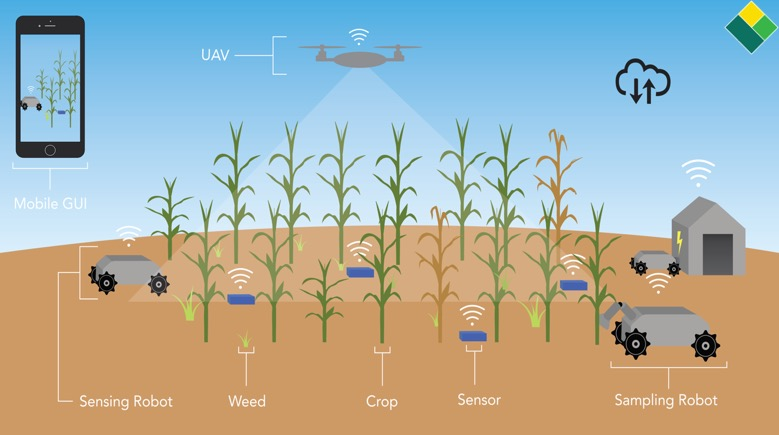
\includegraphics[width=\columnwidth]{agrobot_cps.jpg}
		\caption{A Cyber Physical system consisting of a distributed team of robots for mechanical weed management on a farm. Image courtesy EarthSense inc.}
	\label{fig:cps}
\end{figure}
%With rapid advances in low-cost data processing hardware and mobile robotics, large scale cyber physical systems capable of monitoring 

 %In situations where this is possible, such as in computational fluid dynamics, the resulting models may become computationally intractable, requiring hours or even days on supercomputers, and far out of the reach of compute and connectivity capabilities on robots or sensors deployed in the field.  On the other hand, recent advances in machine learning indicate that perhaps data-driven modeling could be a promising way  .  


%There has been significant interest in developing distributed modeling and monitoring algorithms for such systems, however, 


%The objective of this article is to introduce a modeling and monitoring mechanism that marries together recent successes of machine learning with powerful results from systems and control theory. We achieve this by demonstrating how critical properties such as observability and controllability can be derived systems can be embedded inside feature spaces of machine learning models We now elaborate the context behind this claim.  
% Let us dwell on this point a bit, its rather tempting to dismiss deep learning models and machine learning in general as blackboxes, but one can't argue with the success of those models. Taking a deeper look, one realizes that all machine learning is trying to do is to automatically learn a state-space (termed as the feature space cite our sidebar) which may be nonlinarly generated using other features. Infact sidebar blabla discusses three ways in which one could come up with these features, what the engineering community prefers is the features of the first kind which are physically directly relatable to physical quantities. 
%The success of machine learning in complex problems teaches us that giving up on interpretability allows one to solve very tough problems. SO its not the feature space that's the problem, 
%When one gives up physical interpretability, it becomes rather  difficult to understand why something is broken, or what guarantees could be put in place to ensure performance remains within bounds. with the traditional deep learning models, the only real way of dealing with this right now is sampling based, that is through thousands of simulations. Going a step further, its difficult to come up with guarantees on certain behaviors of the model. Observability and controllability are two fundamental guaratnees that controls interpretable models have provided us. SO the question that we ask here is does embedding interpretable models in complex feature spaces allows us to recover some of those guarantees while leveraging the strength of feature learning.

%Taking a broader perspective, complex dynamical systems such as agriculture and weather are very difficult to model and control using traditional first principles based approaches alone. On the other hand


These types of problems are characterized by complex and stochastic dynamics that are distributed in space and time. %It may be difficult to model such systems with spatiotemporal dynamics using first principles alone. 
While modeling such spatiotemporal phenomena has traditionally been the province of the field of geostatistics, it has in recent years gained more attention in the machine learning community \cite{cressie2011statistics}. The data-driven models developed through machine learning techniques provide a way to capture complex spatiotemporal phenomena which are not easily modeled by first-principles alone. 


 %, such as those described by stochastic partial differential equations with uncertain parameters. %, such as stochastic partial differential equations. 

In the machine learning community, kernel methods represent a class of extremely well-studied and powerful methods for inference in spatial domains; in these techniques, correlations between the input variables are encoded through a covariance kernels, and the model is formed through a linear weighted combination of the kernels \cite{RasmussenWilliams2005,schoelkopf01kernelbased,scholkopf2002learning}. In recent years, kernel methods have been applied to spatiotemporal modeling with varying degrees of success \cite{cressie2011statistics,RasmussenWilliams2005}. Many recent techniques in spatiotemporal modeling have focused on nonstationary covariance kernel design and associated hyperparameter learning algorithms \cite{garg2012AAAI,ma2003nonstationary,plagemann2008nonstationary}. These methods, which focus on the careful design of covariance kernels,  have been proposed as an alternative to the naive approach of  simply including time as an additional input variable in the kernel \cite{Chowdhary13_CDC1}. The careful design/optimization of covariance kernel avoids an explosion in the number of parameters (kernels utilized) of the model which would be inevitable in a model that simply adds time as an additional input variable, and has been shown to better account for spatiotemporal couplings. However, there are two key challenges with existing kernel based approaches: The first is ensuring the scalability of the model to large scale phenomena, which manifests due to the fact that the problem of optimizing the covariance kernel (known as hyperparameter optimization in the ML community) is not convex in general, leading to methods that are difficult to implement especially in online settings, susceptible to getting stuck at local minima, and highly computationally demanding for large datasets. % \cite{sra2012optimization}. 
The second key challenge is in using existing kernel-based machine learning models for analysis and synthesis of observers and controllers for the large scale spatiotemporal phenoemena. While the first challenge can be addressed with increasing computational power for large datasets, addressing the latter (and vastly more fundamental) challenge is particularly important in the design of reliable engineering systems, such as distributed sensor/actuator networks intended for monitoring physical phenomena, autonomous soft-robots, or other physical systems with distributed sensing and actuation.  %Consider in specific the problem of designing an optimal distributed sensor network for ``monitoring'' a spatiotemporally evolving function. 
%Some of the fundamental engineering questions that are of importance here are Given an approximate predictive model of the spatiotemporal phenomena, how can the current latent state of the phenomena be estimated using as few sensor measurements as possible?  
% 
   
%In addition to the challenge of modeling spatiotemporally varying processes, we are interested in addressing the second very important, and widely unaddressed challenge:

%To focus the development of the theory, we posit the challenging problem of ``monitoring'' a spatiotemporal phenoemena: Given an approximate predictive model of the spatiotemporal phenomena, how can the current latent state of the phenomena be estimated using as few sensor measurements as possible? This is called the \emph{monitoring problem}. Monitoring a spatiotemporal phenomenon is concerned with estimating its current state, predicting its future evolution, and inferring the initial conditions utilizing limited sensor measurements. The key challenges here manifest due to the fact that it is typically infeasible or expensive to deploy sensors at a large scale across vast spatial domains. %For example, in monitoring the flux of $CO_2$ over underground $CO_2$ storage sites, the number of sensors and sensing locations are limited due to cost or geography. %In another example, when monitoring the state of dynamically evolving enemy deployment over a contested area, the availability of measurements is limited due to the presence of adversity.
%To minimize the number of sensors deployed, a predictive data-driven model of the spatiotemporal evolution could be learned from historic datasets or through remote sensing  (e.g. satellite, radar) datasets. Then, to monitor the phenomenon, the key problem would boil down to reliably and quickly estimate the evolving latent state of the phenomena utilizing measurements from very few sampling locations.

%The problem of state estimation of a temporally evolving finite-dimensional state-space system has been extensively studied in the dynamical systems and feedback-control community \cite{Gelb74}. Fundamental results in systems observability theory provide sufficient conditions on the structure of the state transition and measurement matrix such that the latent state can be tracked with a measurement-feedback observer using a number of measurements less than the number of states. A highly successful example of such a state estimator is the celebrated Kalman filter, which is a Bayes-optimal filter for estimating the latent states of a finite-dimensional linear state-space model corrupted with Gaussian noise \cite{Gelb74}. Such filters can be extended to the functional domain \cite{mardia1998kriged}, but are typically not studied in a monitoring context. 


\subsection{Contributions}
In this article, we present a new perspective to solving the spatiotemporal monitoring problem that brings together kernel-based modeling, systems theory, and Bayesian filtering. We define the monitoring problem as follows: \textit{Given an approximate predictive model of the spatiotemporal phenomena learned using historic data, estimate the current latent state of the phenomena in the presence of uncertainty using as few sensors as possible}. In particular, we argue that when it comes to predictive inference over spatiotemporal phenomena, a Kalman-filter type approach of predicting and correcting with feedback from a set of minimal sensors is a robust way of dealing with real-world uncertainties and inherent modeling errors.  In the context of this specific problem, our \textit{main contributions are two-fold}: first, we demonstrate that spatiotemporal functional evolution can be modeled using stationary kernels with a linear dynamical systems layer on their mixing weights. In particular, in contrast with existing work, this approach does not necessarily require the design of complex spatiotemporal kernels, and can accommodate positive-definite kernels on any domain on which it is possible to define them, which includes non-Euclidean domains such as Riemannian manifolds, strings, graphs and images \cite{Jayasumana_PAMI2015_RBFs}. Second, we show that such a model can be utilized to determine sensing locations that guarantee that the hidden states of functional evolution can be estimated using a Bayesian state-estimator (Kalman filter) with very few measurements. We provide sufficient conditions on the number and location of sensor measurements required and prove non-conservative lower bounds on the minimum number of sampling locations by developing fundamental results on observability of kernel based models. The validity of the presented model and sensing techniques is corroborated using synthetic and large real datasets. (MENTION DNNS)

\subsubsection*{Broader Context}
The fundamental idea of building observers and controllers introduced in this paper is generalizable beyond the particular application of spatiotemporal monitoring. Indeed, the significance of the contributions of this paper are in fusing machine learning theory with systems theory to provide a pathway to address major challenges in distributed monitoring and control of complex spatiotemporally varying systems. 


\begin{figure}[h] %{r}{0.5\textwidth}
	\centering
	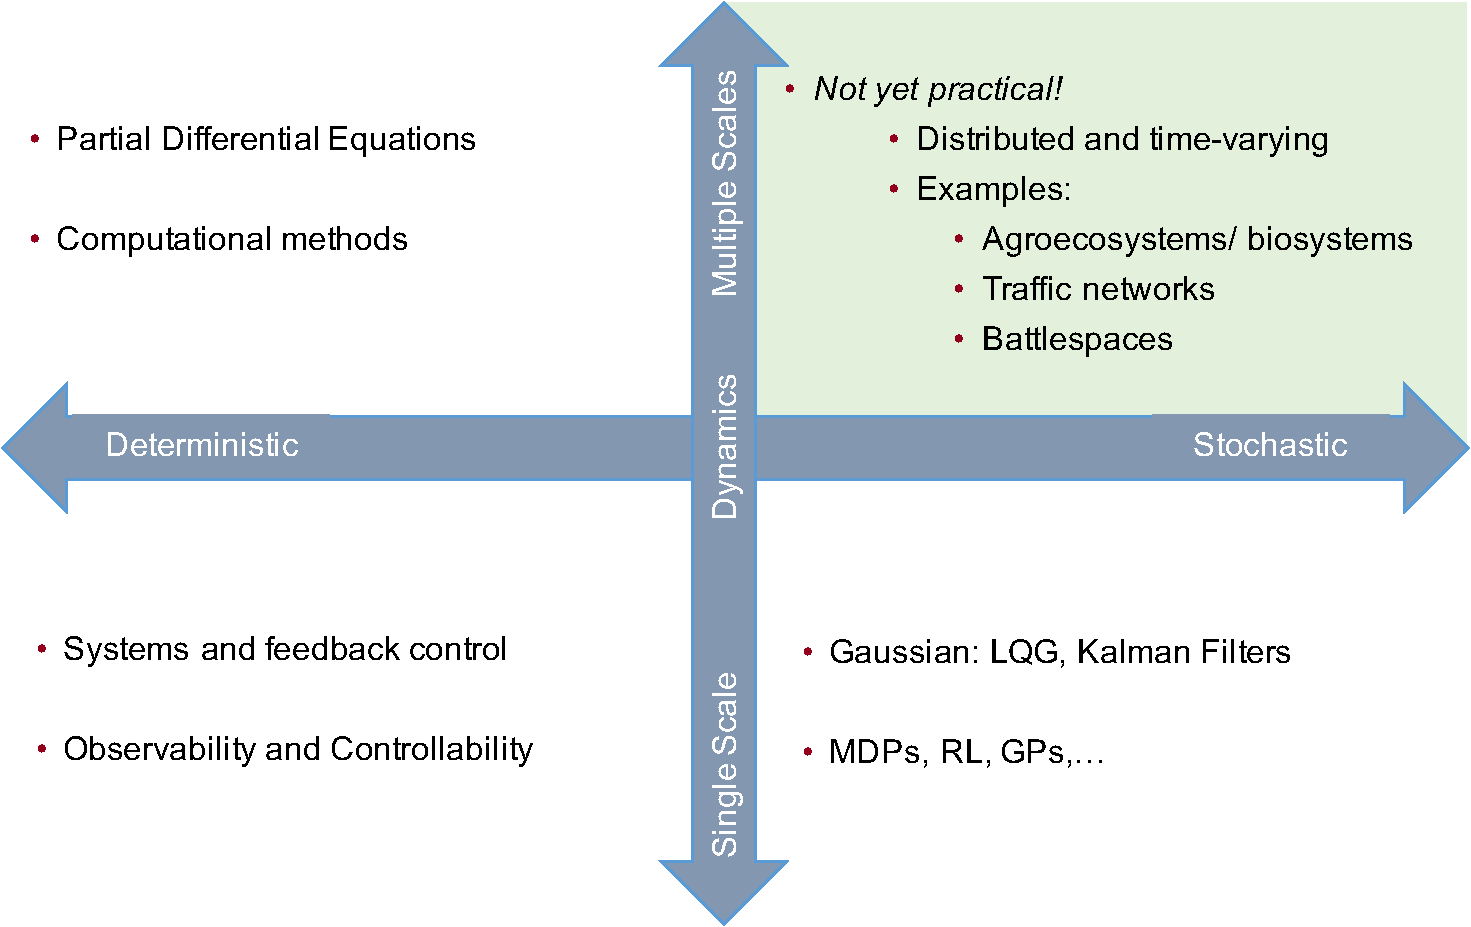
\includegraphics[width=\columnwidth]{CPS_SOA}
		\caption{Modeling, monitoring, and controlling dynamical systems with complex and uncertain dynamics, such as agricultural, traffic, or weather monitoring systems, presents exciting open challenge for the controls community. The bottom left quadrant describes linear and time-invariant systems with single- scale dynamics, for which the theory of feedback control of dynamical systems is often sufficient. The bottom right quadrant shows stochastic single-scaled systems, where approaches such as Kalman Filters and Gaussian optimization have marked several successes of control systems enabling endeavors from Lunar landings to GPS navigation. The top left quadrant denotes systems with dynamics at multiple scales, where efficient computational solutions to Partial Differential Equations (PDEs) is an highly active area of research. However, fundamental theoretical advances and practical algorithms are needed to enable autonomous decision making for distributed stochastic Cyber Physical Systems with dynamics at multiple scales – shown in the top right quadrant – such as distributed agricultural robotic systems, traffic networks, and weather monitoring systems with mobile and stationary sensors.}
	\label{fig:cps_soa}
\end{figure}
%Complex spatiotemporally varying systems such as agricultural systems, weather patterns, or fluid flows are typically difficult to address with traditional controls model with
  
Traditionally, the controls literature is strongest when the system dynamics can be represented as ODEs. % (see for example Figure \ref{fig:cps_soa}. Indeed %has focused on first principles and physics based models. As 
As depicted in Figure \ref{fig:cps_soa}, some of the major successes of controls have included results such as LQG, reinforcement learning, and adaptive control in finite, well-defined, and physically meaningful state spaces. The problem of state estimation of a temporally evolving, finite-dimensional state-space system for example has been extensively studied in the context of Kalman filtering and observer design \cite{Gelb74}. Here, fundamental results in observability/controllability provide sufficient conditions on the structure of the state transition and measurement matrix such that the latent state can be estimated in the presence of measurement and process noise. %A highly successful example of such a state estimator is the celebrated Kalman filter, which is a Bayes-optimal filter for estimating the latent states of a finite-dimensional linear state-space model corrupted with Gaussian noise \cite{Gelb74}. 
Such filters can be naively extended to the functional domain (e.g.\cite{mardia1998kriged}), but have not typically been studied in context of the spatiotemporal monitoring problem studied here.  


On the other hand, recent advances in machine learning are providing different and highly powerful ways of modeling complex spatiotemporal dynamical systems.  %Yet %the sheer complexity of agricultural systems or weather patterns can make it difficult to design meaningful mo first principles based modeling highly limiting. Recent advances in machine learning would indicate that perhaps data-driven modeling could be very promising. 
Yet, the main challenge with using machine learning approaches such as deep learning or kernel based methods has been that these approaches lack interpretablity and analyzability, which makes it difficult to design robust engineered systems. This is mostly because machine learning works in abstract feature spaces that are sometimes not directly relatable to physical quantities (see Sidebar \ref{sb:featspace} for discussion on feature spaces in machine learning). For example, when kernel based models are used for spatiotemporal systems, how does one answer fundamental questions such as 1) the least number of sensors required to observe a distributed system, 2) the placement of sensors/actuators to guarantee observability/controllability of the system, and 3) the effect of random sensor placement on system observability/controllability.

In this paper we present an approach that can provide a formal way of addressing these and other questions about complex systems that are modeled with machine learning. In particular, we demonstrate how linear dynamical systems can be embedded in machine learning feature spaces and utilized to answer fundamental questions such as controllability and observability.  This marriage of systems theory with machine learning pursued in this paper is exciting, and % because it can provide a formal way of answering fundamental questions about complex systems, such as: % and seek to develop machine learning models that can be utilized to answer questions such as: 
 we expect that follow-up work will exploit the framework presented in this paper of utilizing linear models in feature spaces of machine learning models to enable practical and analyzable data-driven engineering systems. To facilitate the development of the theory, we have focused this paper on the problem of monitoring spatiotemporal phenomena. However, the idea can be generalized to any distributed cyber-physical system that is changing with space and time. %As such, we have focused mostly on the fundamental theory and practical algorithms in modeling, estimation, and control, while 
%The excruciating details of how to optimally implement the presented algorithms are omitted\footnote{Instead an open-source code-base is made available in MATLAB on http://daslab.illinois.edu/software.html and in Python on GitHub https://github.com/hkingravi/funcobspy?files=1}.   % that are analyzable.

Elements of the work presented in this paper first appeared in the premier machine learning conference Neural Information Processing Systems (NIPS 2016) (\cite{Kingravi16_NIPS,whitman2016NIPSworkshop}), IEEE CDC 2015 conference \cite{Kingravi:2015a}, the Conference on Robot Learning (CoRL 2017) \cite{whitman2017learning} and IEEE ACC 2018 conference \cite{Maske18_ACC}.  This paper presents a comprehensive set of results in a single journal publication, and introduces results on observability in the presence of random sensor placement. As such, we have focused in this article mostly on the fundamental theory and practical algorithms for modeling, estimation, and control, while the excruciating details of how to optimally implement the presented algorithms are omitted\footnote{Instead an open-source code-base is made available in MATLAB on http://daslab.illinois.edu/software.html and in Python on GitHub https://github.com/hkingravi/funcobspy?files=1}. Section \ref{sec:related} summarizes some related work in machine learning in this area. Sidebar \ref{sb:featspace} outlines feature spaces in machine learning in a broader context. Section \ref{sec:observers} formulates the problem,  introduces \emph{Kernel Observers (KO)}, and develops the main theoretical and algorithmic results.
Section \ref{sec:random_results} presents a result on the expected number of randomly placed sensors required to monitor a spatiotemporal process in the context of our model. Section \ref{sec:egp} presents an extension to the KO method called \emph{Evolving Gaussian Processes (E-GP)} that learns one model for multiple, similar spatiotemporal processes. The efficacy of this approach on real-world CFD data is presented in \ref{sb:cfd}.
The paper is concluded in Section \ref{sec:conclusion}. 

%Section \ref{sec:exp} demonstrates the efficacy of the algorithms on several challenging and large real-world datasets.  and proofs of main results are provided in the Appendix. (IS THERE AN APPENDIX?)
\subsection{Related Work}\label{sec:related}
There is a large body of literature on spatiotemporal modeling in geostatistics where specific process-dependent kernels can be used \cite{wikle2002kernel,cressie2011statistics}. From the machine learning perspective, a naive approach is to utilize both spatial and temporal variables as inputs to a Mercer kernel \cite{perez2013gaussian}. However, this technique leads to an ever-growing kernel dictionary. %, which is computationally taxing.
Furthermore, constraining the dictionary size or utilizing a moving window will
occlude learning of long-term patterns. Periodic or nonstationary covariance functions and nonlinear transformations have been proposed to address this issue \cite{ma2003nonstationary,RasmussenWilliams2005}. Work focusing on nonseparable and nonstationary covariance kernels seeks to design kernels optimized for environment-specific dynamics, and to tune their hyperparameters in local regions of the input space. Seminal work in \cite{higdon1998process} proposes a process convolution approach for space-time modeling. This model captures nonstationary structure by allowing the convolution kernel to vary across the input space. This approach can be extended to a class of nonstationary covariance functions, thereby allowing the use of a Gaussian process (GP) framework, as shown in \cite{paciorek2004nonstationary}. However,  since this model's hyperparameters are inferred using MCMC integration, its application has been limited to smaller datasets. To overcome this limitation, \cite{plagemann2008nonstationary} proposes to use the mean estimates of a second isotropic GP (defined over latent length scales) to parameterize the nonstationary covariances. Finally, \cite{garg2012AAAI} considers non-isotropic variation across different dimension of input space for the second GP as opposed to isotropic variation by \cite{plagemann2008nonstationary}. Issues with this line of approach include the nonconvexity of the hyperparameter optimization problem and the fact that selection of an appropriate nonstationary covariance function for the task at hand is a nontrivial design decision (as noted in \cite{singh2010modeling}). 

Apart from directly modeling the covariance function using additional latent GPs, there exist several other approaches for specifying nonstationary GP models. One approach maps the nonstationary spatial process into a latent space, in which the problem becomes approximately stationary \cite{schmidt2003bayesian}. Along similar lines, \cite{pfingsten2006nonstationary} extends the input space by adding latent variables, which allows the model to capture  nonstationarity in original space. Both these approaches require MCMC sampling for inference, and as such are subject to the limitations mentioned in the preceding paragraph. 

%The geostatistics community literature has many examples of the dynamical spatiotemporal modeling approach, where the focus is on finding good dynamical transition models on the linear combination of weights in a parameterized model \cite{cressie2011statistics,mardia1998kriged}. 
A geostatistics approach that finds dynamical transition models on the linear combination of weights of a parameterized model \cite{cressie2011statistics,mardia1998kriged} is advantageous when the spatial and temporal dynamics are hierarchically separated, leading to a convex learning problem. As a result complex nonstationary kernels are often not necessary (although they can be accommodated). The approach presented in this paper aligns closely with this vein of work. %The main difference is that we view the problem from the more abstract viewpoint of constructing an observer in a reproducing kernel Hilbert space. 
A systems-theoretic study of this viewpoint enables the fundamental contributions of the paper, which are 1) allowing for inference on more general domains with a larger class of basis functions than those typically considered in the geostatistics community, and 2) quantifying the minimum number of measurements required to estimate the state of the system. 

Lastly, sensor placement optimization is also a well-studied area. Examples include, but are not limited to 1) geometric approaches, which seek to provide a covering of the operating space without making assumptions about the spatiotemporal dynamics \cite{egerstedt:bk:2010}, and 2) information-theoretic approaches, which place their focus on sensor placement optimizing strategies based on mutual information and information entropy for Gaussian process models \cite{Guestrin05_ICML}.
It should be noted that the contribution of the paper concerning sensor placement is to provide \emph{sufficient conditions} for monitoring rather than optimization of the placement locations, and therefore a comparison with these approaches is not considered in the experiments. 


\vspace{-0.1in}
\section{Kernel Observers}\label{sec:observers}
This section outlines our modeling framework and presents theoretical results associated with the number of sampling locations required for monitoring functional evolution. 
\vspace{-0.1in}
\subsection{Problem Formulation}\label{sec:formulation}
We focus on predictive inference of a time-varying stochastic process, whose mean $f$ evolves temporally as $f_{\tindex+1} \sim \mathbb{F}(f_{\tindex},\eta_{\tindex})$, where $\mathbb{F}$ is a distribution varying with time $\tindex$ and exogenous inputs $\eta$. Our approach builds on the fact that in several cases, temporal evolution can be hierarchically separated from spatial functional evolution. A classical and quite general example of this is the \emph{abstract evolution equation} (AEO), which can be defined as the evolution of a function $\banachfunc$ embedded in a Banach space $\banachspace$: $\dot{\banachfunc}(t) = \banachop\banachfunc(t)$, subject to $\banachfunc(0)= \banachfunc_0$, and $\banachop:\banachspace\to\banachspace$ determines spatiotemporal transitions of $\banachfunc\in\banachspace$ \cite{brezis2010functional}. This model of spatiotemporal evolution is very general (AEOs, for example, model many PDEs), but working in Banach spaces can be computationally taxing.  A simple way to make the approach computationally realizable is to place restrictions on $\banachspace$: in particular, we restrict the sequence $f_{\tindex}$ to lie in a reproducing kernel Hilbert space (RKHS), the theory of which provides powerful tools for generating flexible classes of functions with relative ease \cite{RasmussenWilliams2005}.
In a kernel-based model, $\kernel:\dom\times\dom\to\R$ is a positive-definite Mercer kernel on a domain $\dom$ that models the covariance between any two points in the input space,  
and implies the existence of a smooth map $\fmap:\dom\to\fspace$, where $\fspace$ is an RKHS with the property $\kernel(x,y) = \Kiprod{x}{y}$. The key insight behind the proposed model is that spatiotemporal evolution in the input domain corresponds to temporal evolution of the mixing weights of a kernel model alone in the functional domain. Therefore, $f_{\tindex}$ can be modeled by tracing the evolution of its mean embedded in a RKHS using switched ordinary differential equations (ODE) when the evolution is continuous, or switched difference equations when it is discrete (Figure \ref{fig:hilbert_evolution}). 
The advantage of this approach is that it allows us to utilize powerful ideas from systems theory for deriving necessary and sufficient conditions for spatiotemporal monitoring. 
\begin{figure}
\centering
\begin{minipage}{0.45\textwidth}
\centering
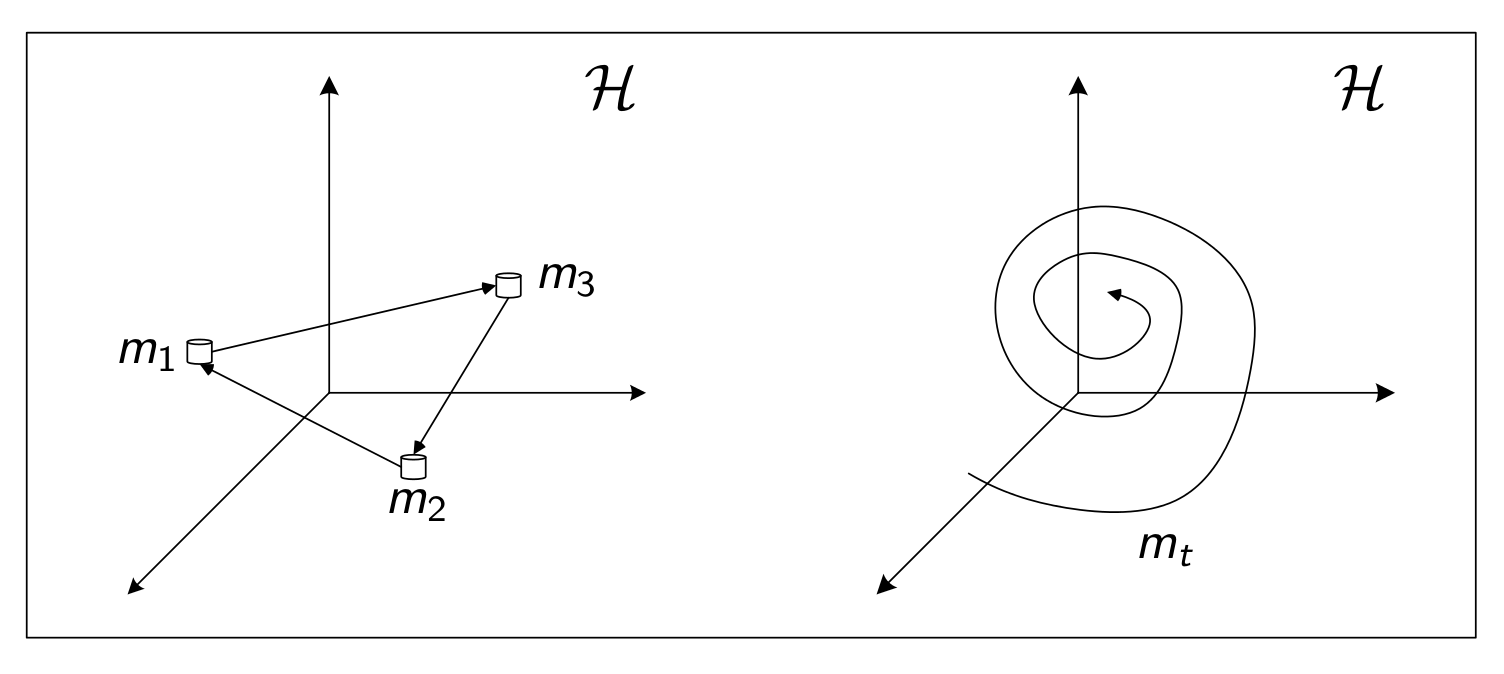
\includegraphics[height=1.0in]{figures/model.png}
\caption{\small{Two types of Hilbert space evolutions. Left: discrete switches in RKHS $\fspace$; Right: smooth evolution in $\fspace$.}}
\label{fig:hilbert_evolution}           
\end{minipage}\hfill
\begin{minipage}{0.45\textwidth}
\centering
\subfloat[\small{1-shaded (Def. \ref{def:shaded})}]{
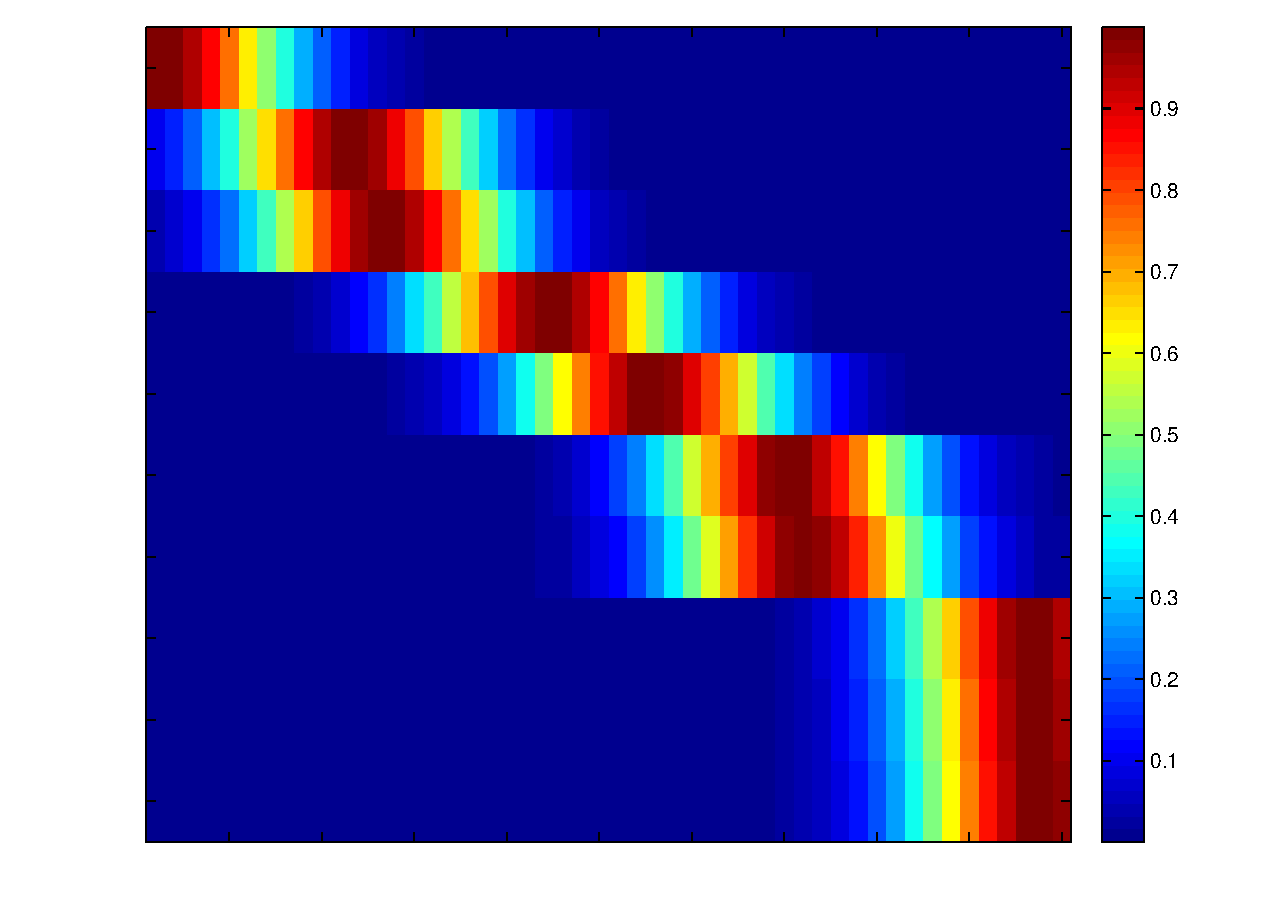
\includegraphics[width=0.47\columnwidth]{shaded_kmat.pdf} \label{fig:shadeda}}
\subfloat[\small{2-shaded (Eq. \eqref{empKShadFull})}]{
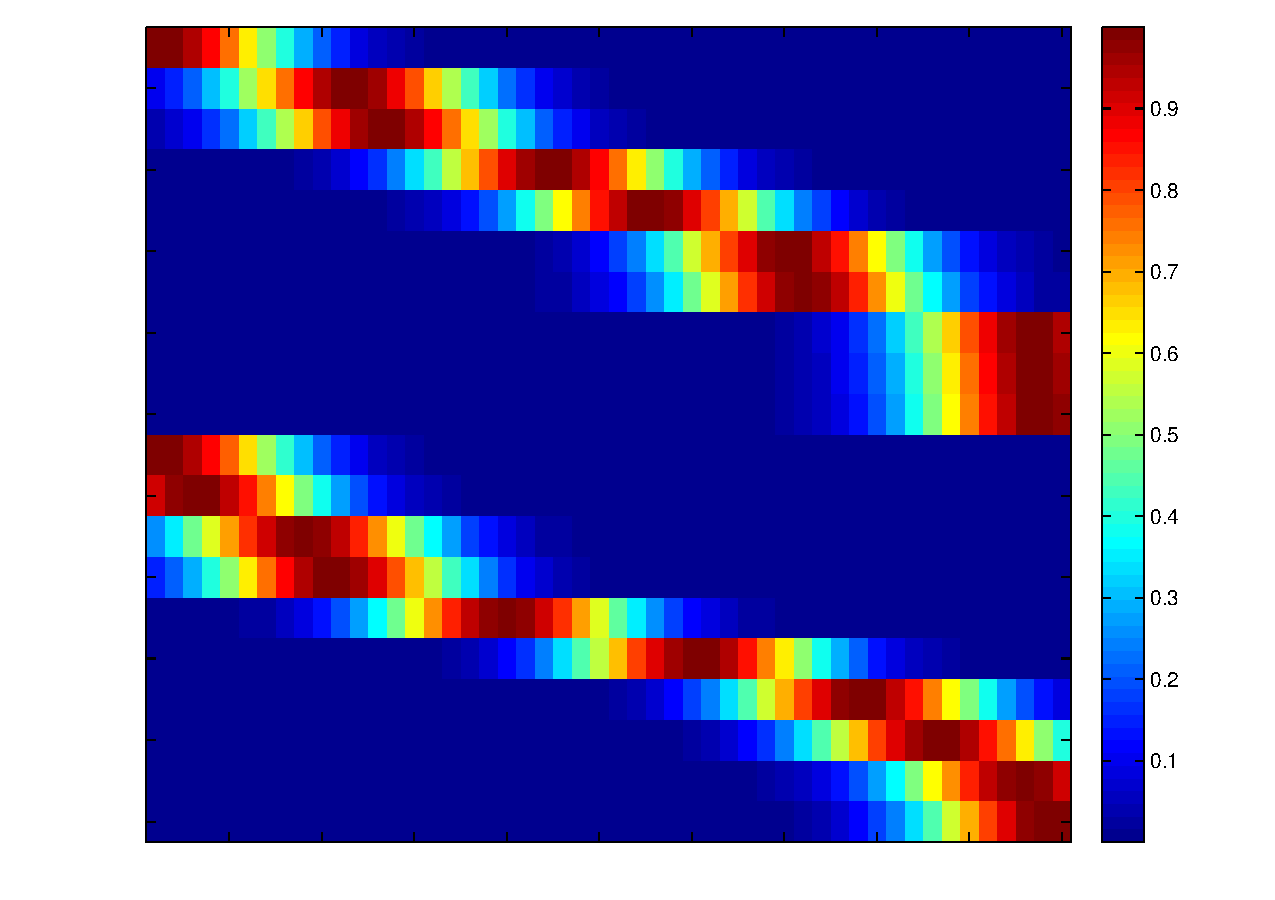
\includegraphics[width=0.47\columnwidth]{shaded_kmat_multiple.pdf} \label{fig:shadedb}}
\caption{\small{Shaded observation matrices for dictionary of atoms. Each row represents a sensing location with the color map indicating the evaluation of kernel function w.r.t the others points in the domain.}}
\label{fig:shaded}
\end{minipage}
\end{figure}
% \begin{figure}
%  \centering
%  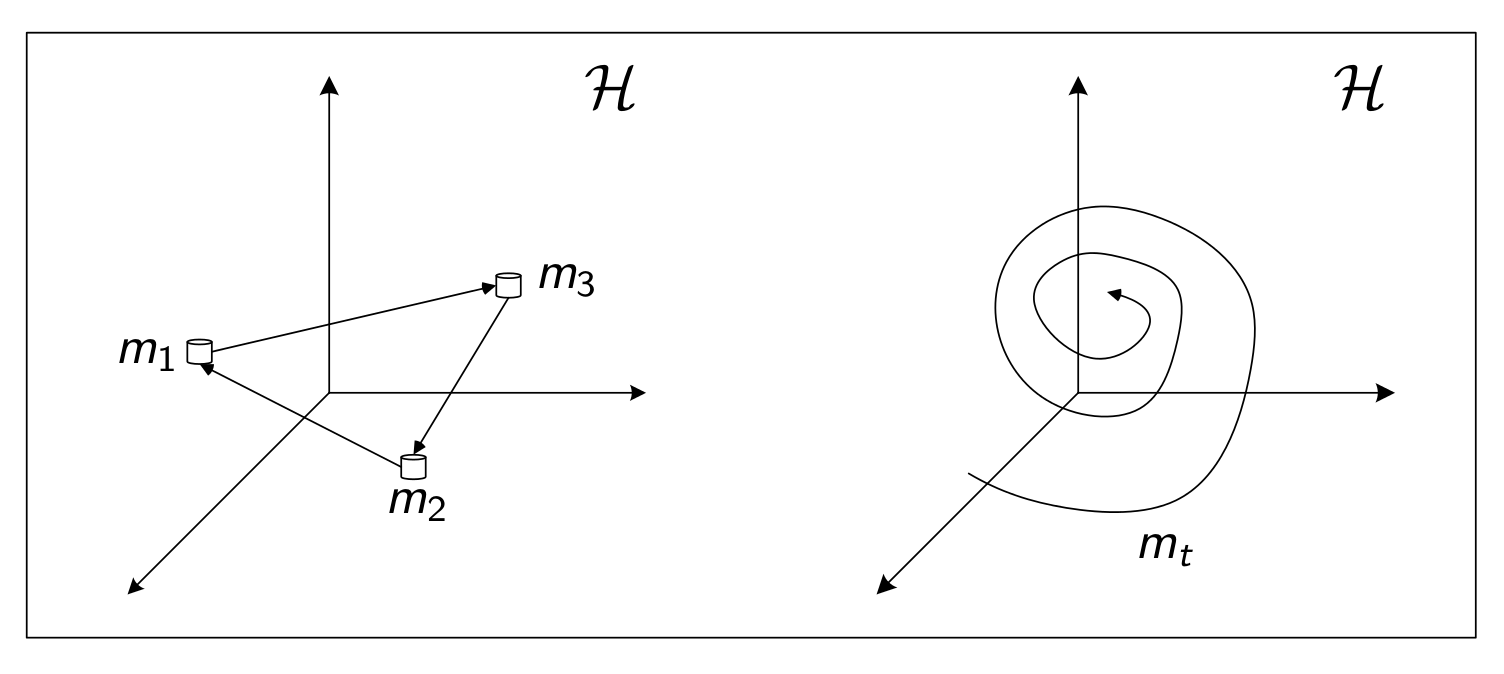
\includegraphics[height=2.0in]{figures/model.png}
% \caption{\small{Two types of Hilbert space evolutions. Left: discrete switches in RKHS $\fspace$; Right: smooth evolution in $\fspace$.}}
% \label{fig:hilbert_evolution}
% \end{figure} 
% \begin{figure}
%  \centering
%  \subfloat[\small{1-shaded (Definition \ref{def:shaded})}]{
% 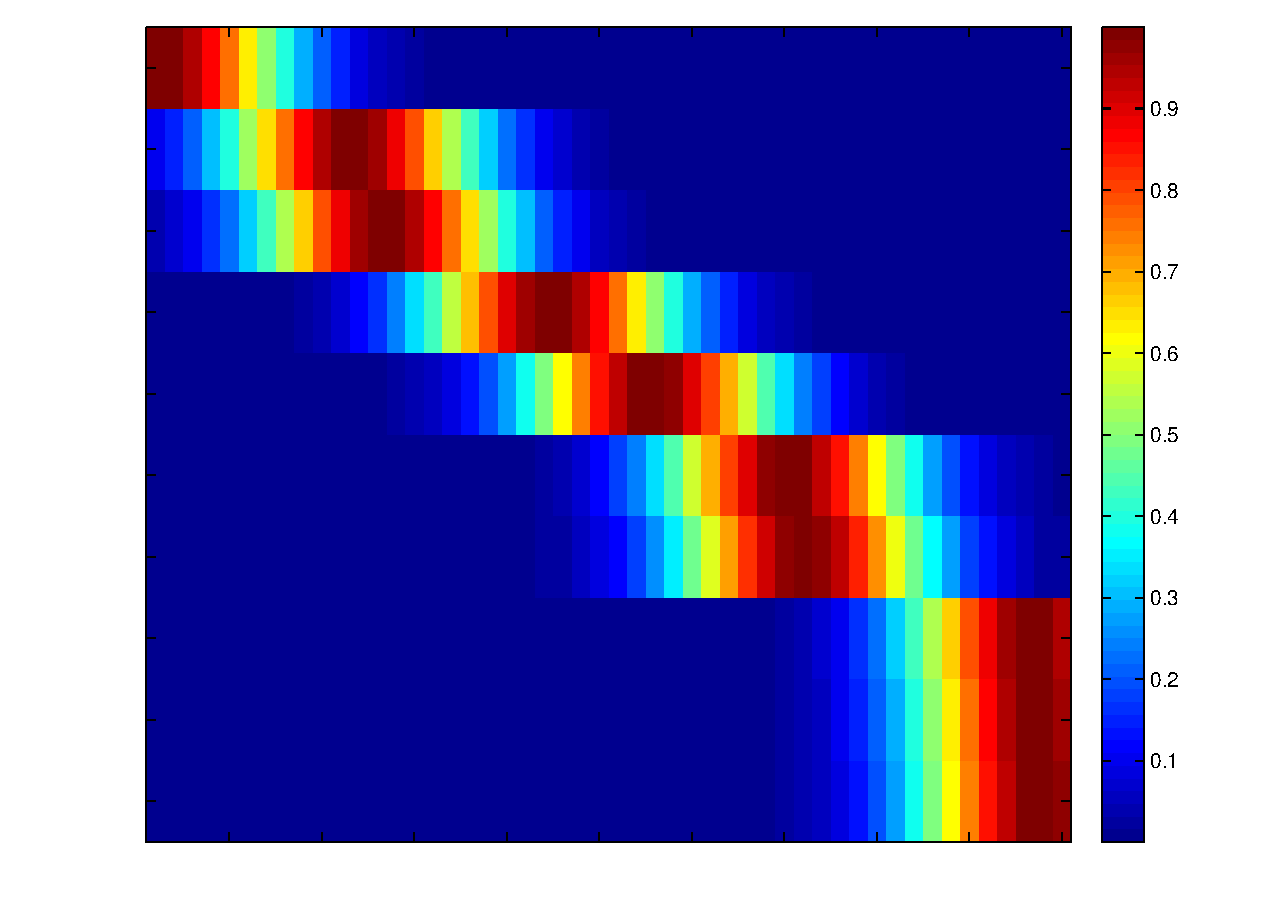
\includegraphics[width=0.4\columnwidth]{shaded_kmat.pdf} \label{fig:shadeda}}
% \subfloat[\small{2-shaded (Eq. \eqref{empKShadFull})}]{
% 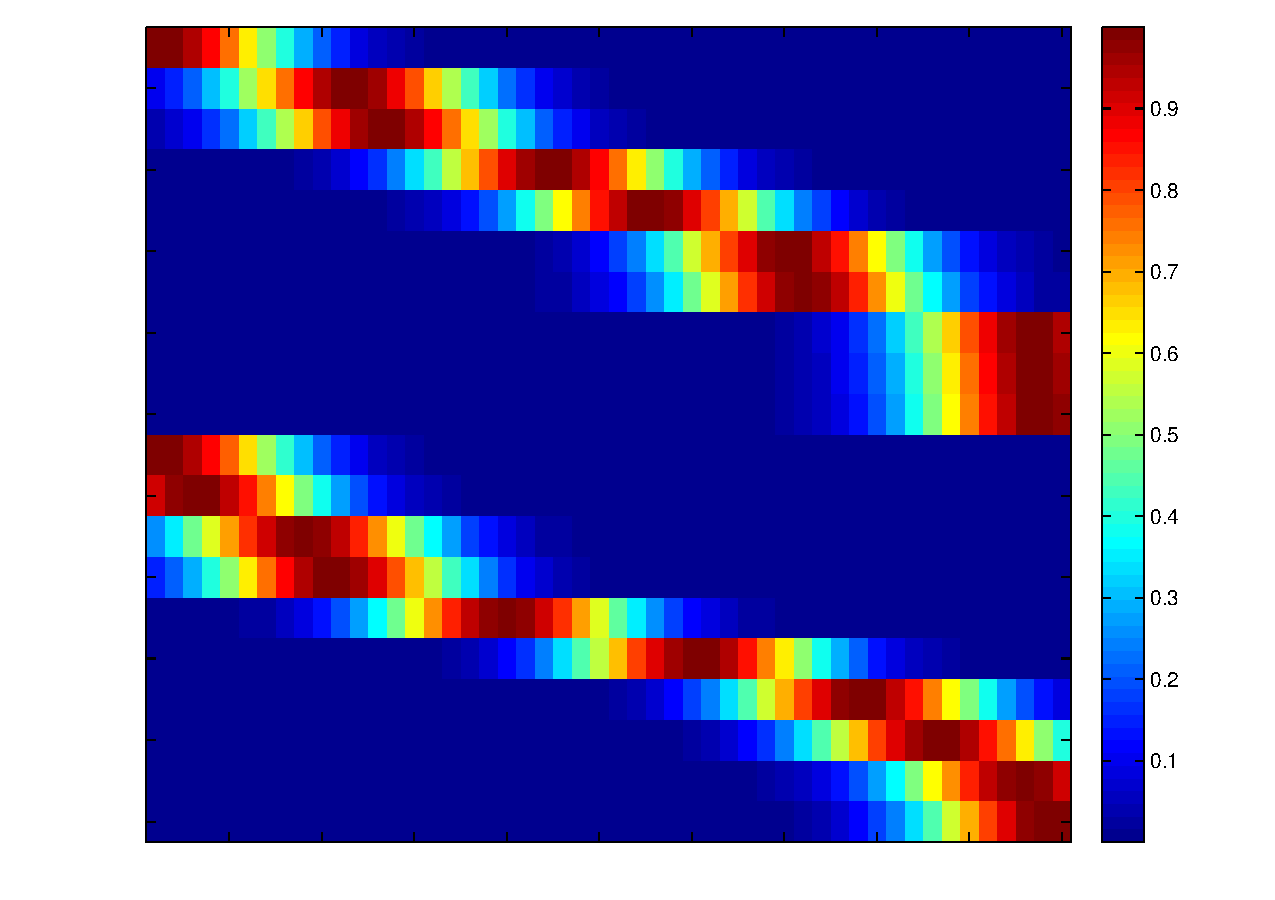
\includegraphics[width=0.4\columnwidth]{shaded_kmat_multiple.pdf} \label{fig:shadedb}}
% \caption{\small{Shaded observation matrices for dictionary of atoms.}}
% \label{fig:shaded}
% \end{figure}

\begin{figure}[t]
\centering
\subfloat[\small{Gaussian}]{
 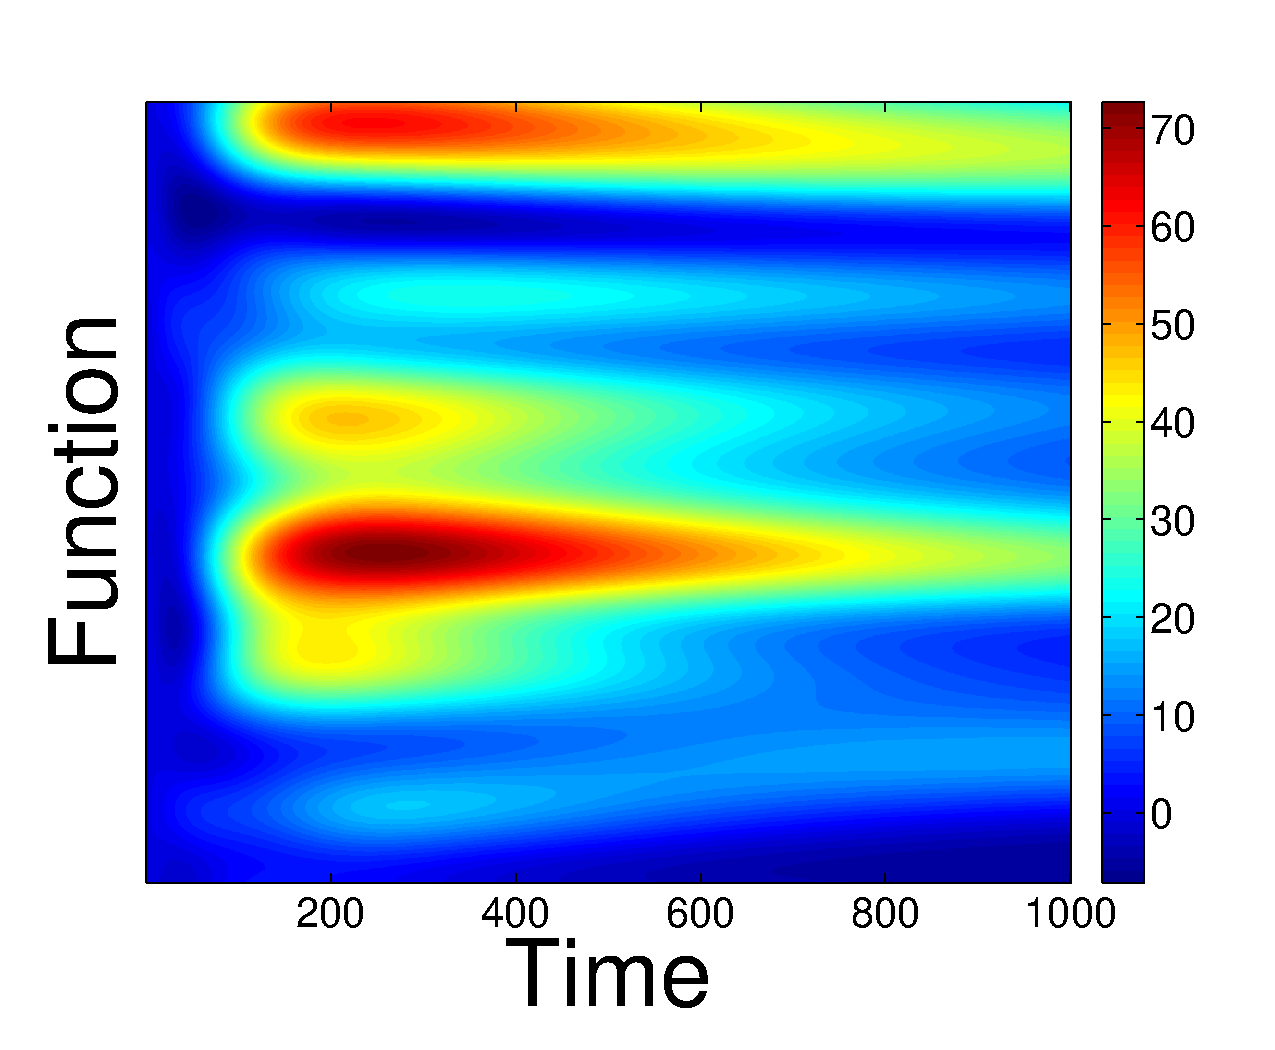
\includegraphics[width=0.25\columnwidth]{figures/kernel_evol_gaussian.pdf}
}
\subfloat[\small{Laplacian}]{
 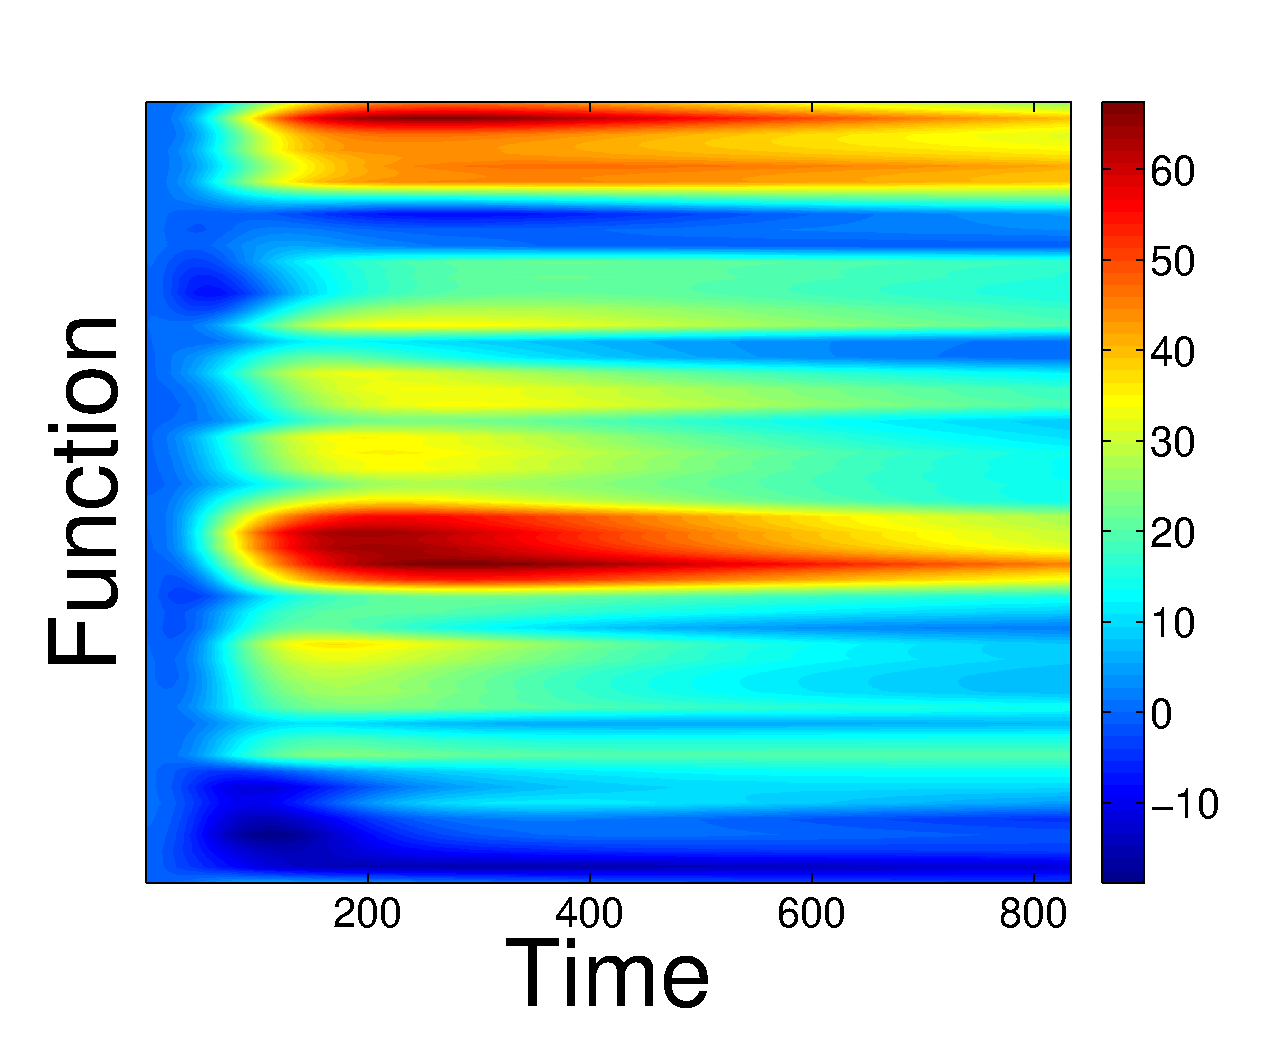
\includegraphics[width=0.25\columnwidth]{figures/kernel_evol_laplacian.pdf}
}
% \\
\subfloat[\small{Periodic}]{
 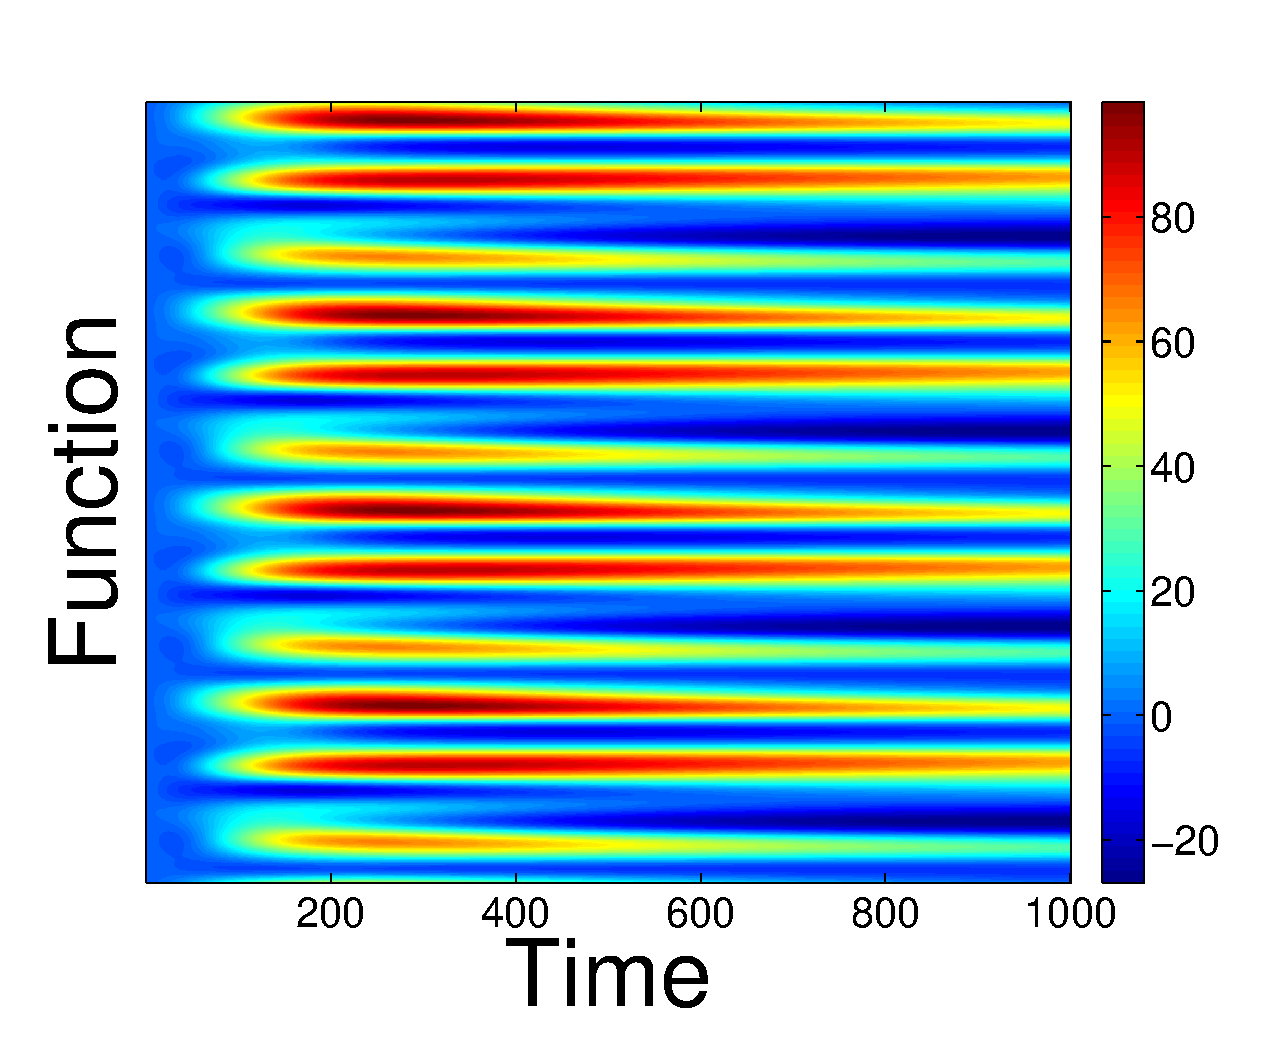
\includegraphics[width=0.25\columnwidth]{figures/kernel_evol_periodic.pdf}
}
% \subfloat[\small{Locally periodic}]{
%   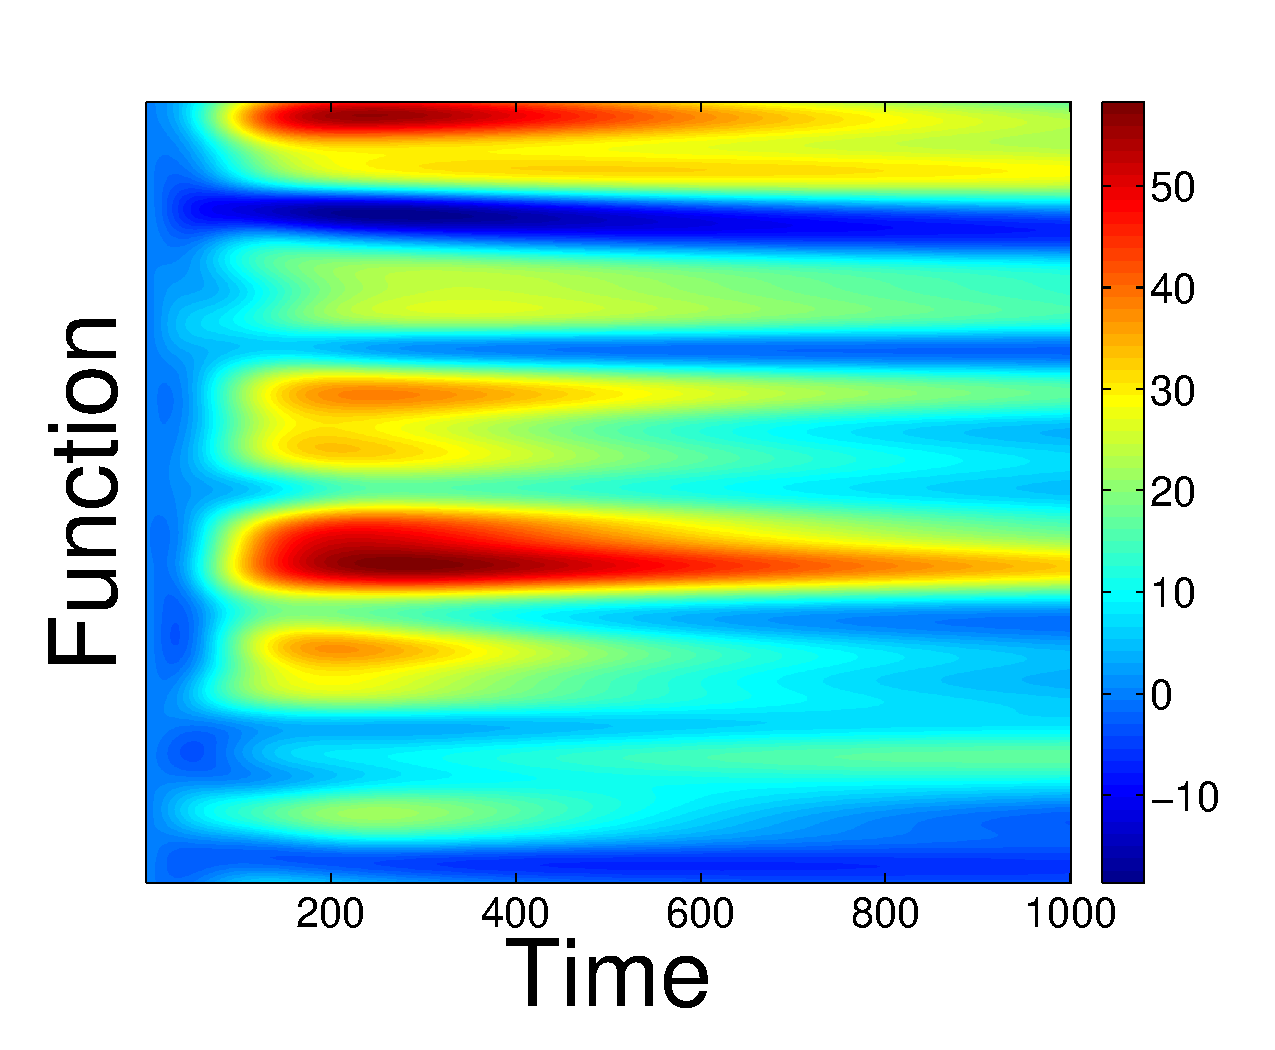
\includegraphics[width=0.3\columnwidth]{figures/kernel_evol_locally_periodic.pdf}
%}
\caption{\small{One-dimensional function evolution over a fixed transition matrix $A$, 
initial condition $\weight_0$ and centers $\shCent$, but with different kernels $\kernel(x,y)$. 
Each $y$-vector at a given value of $x$ represents the output of the function, which evolves from left to right. 
As seen, changing the kernel creates quite different dynamic behaviors. }%behavior for the same system.}
}
\label{fig:kernel_variation}
\end{figure}
In this paper, we restrict our attention to the class of functional evolutions $\mathbb{F}$ defined by linear Markovian transitions in an RKHS. While extension to the nonlinear case is possible (and non-trivial), it is not pursued in this paper to help ease the exposition of the key ideas. The class of linear transitions in RKHS is rich enough to approximately model many real-world datasets, as suggested by our experiments.

Let $y\in\R^{\nsamp}$ be the measurements of the function available from $\nsamp$ sensors, $\sysop:\fspace\to\fspace$ be a linear transition operator in the RKHS $\fspace$, and $\measop:\fspace\to\R^{\nsamp}$ be a linear measurement operator. The model for the functional evolution and measurement studied in this paper is:
\begin{align}\eqlabel{ideal_lin_evol}
 f_{\tindex+1} = \sysop f_{\tindex} + \eta_{\tindex}, \quad
 y_{\tindex} = \measop_{\tindex} f_{\tindex} + \zeta_{\tindex},
\end{align}
where $\eta_{\tindex}$ is a zero-mean stochastic process in $\fspace$, and $\zeta_{\tindex}$ is a Wiener process in $\R^{\nsamp}$. 
Classical treatments of kernel methods emphasize that for most kernels, the feature map $\fmap$ is unknown, and possibly infinite-dimensional; this forces practioners to work in the dual space of $\fspace$, whose dimensionality is the number of samples in the dataset being modeled. This conventional wisdom precludes the use of kernel methods for most tasks involving modern datasets, which may have millions and sometimes billions of samples \cite{rahimi2007random}. An alternative is to work with a feature map 
$\fmapApprox(x) := \left[\begin{smallmatrix}
  \fmapApprox_1(x) & \cdots & \fmapApprox_{\ncent}(x)
 \end{smallmatrix}\right]^T$ to an approximate feature space
 $\fspaceApprox$, with the property that for every element $\fspaceEl\in\fspace$, $\exists\fspaceApproxEl\in\fspaceApprox$ and an $\e >0$ s.t. $\|\fspaceEl-\fspaceApproxEl\| < \e$ for an appropriate function norm. A few such approximations are listed below.
%\begin{enumerate}
\paragraph{Dictionary of atoms} Let $\dom$ be compact. Given points $\shCent = \shCentLong$, $c_i\in\dom$, we have a dictionary of atoms $\Atoms = \{\fmap(c_1), \cdots , \fmap(c_{\ncent})\}$, $\fmap(c_i)\in\fspace$, the span of which is a strict subspace $\fspaceApprox$ of the RKHS $\fspace$ generated by the kernel. Here, 
 \begin{equation}\eqlabel{fmap_dict}
 \fmapApprox_i(x) := \l\fmap(x), \fmap(c_i)\r_{\fspace} = \kernel(x, c_i).
 \end{equation}
\paragraph{Low-rank approximations} Let $\dom$ be compact, let $\shCent = \shCentLong$, $c_i\in\dom$, and let $\empK\in\R^{\ncent\times\ncent}$, $\empK_{ij}:=\kernel(c_i,c_j)$ be the Gram matrix computed from $\shCent$. This matrix can be diagonalized to compute approximations $(\empEval_i, \empEfunc_i(x))$ of the eigenvalues and eigenfunctions $(\eval_i, \efunc_i(x))$ of the kernel \cite{williams2001using2}. These spectral quantities can then be used to compute  $ \fmapApprox_i(x):=\sqrt{\empEval}_i\empEfunc_i(x)$.
 \paragraph{Random Fourier features} Let $\dom\subset\R^n$ be compact, and let $ \kernel(x,y) = e^{-\|x-y\|^2/2\s^2}$ be the Gaussian RBF kernel. Then random Fourier features approximate the kernel feature map as $\fmapApprox_{\randFreq}:\dom\to\fspaceApprox$, where $\randFreq$ is a sample from the Fourier transform of $\kernel(x,y)$, with the property that $\kernel(x,y) = \E_{\randFreq}[\l\fmapApprox_{\randFreq}(x),\fmapApprox_{\randFreq}(y)\r_{\fspaceApprox}]$ \cite{rahimi2007random}. In this case, if $\randMat\in\R^{M/2\times n}$ is a random matrix representing the sample $\randFreq$, then 
 $ 
  \fmapApprox_i(x) := \left[\begin{smallmatrix}
  \frac{1}{\sqrt{\ncent}}\sin([\randMat x]_i), \frac{1}{\sqrt{\ncent}}\cos([\randMat x]_i)
 \end{smallmatrix}\right]$. Similar approximations exist for other radially symmetric kernels, as well as dot-product kernels. 

\begin{figure}
\centering
\subfloat[Relationship between $\sysop$ and $A$]{
\label{fig:commute_sysop_dyn}
%\resizebox{0.3\columnwidth}{0.06\paperheight}{%
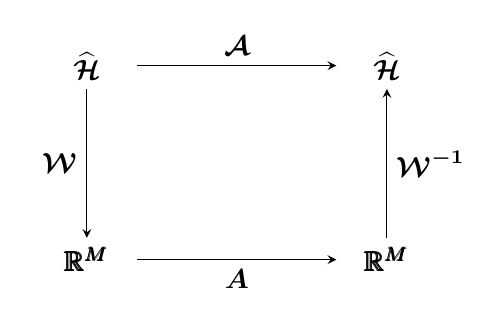
\begin{tikzpicture}
  \matrix (m) [ampersand replacement=\&, matrix of math nodes, 
                 row sep=0.75in,column sep=1in,minimum width=0.5in] {
     \boldsymbol\fspaceApprox \& \boldsymbol\fspaceApprox \\
     \pmb{\R^{\ncent}} \& \pmb{\R^{\ncent}} \\};
  \path[-stealth]
    (m-1-1) edge node [left] {$\boldsymbol\weightmap$} (m-2-1)
            edge [right] node [above] {$\boldsymbol\sysop$} (m-1-2)
    (m-2-1.east|-m-2-2) edge node [below] {$\boldsymbol A$} node [above] {} (m-2-2)
    (m-2-2) edge node [right] {$\boldsymbol\weightmapI$} (m-1-2);            
\end{tikzpicture}  
%}% end resize box
}% end subfloat
\
\subfloat[Relationship between $\measop$ and $\empK$]{
\label{fig:commute_sysop_meas}
%\resizebox{0.3\columnwidth}{0.06\paperheight}{%
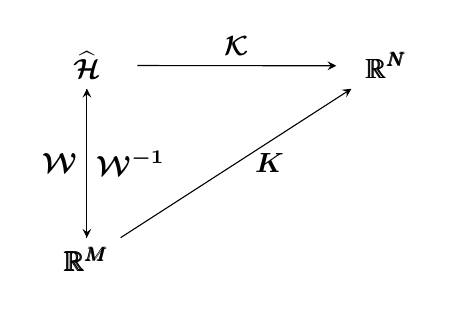
\begin{tikzpicture}
  \matrix (m) [ampersand replacement=\&, matrix of math nodes, 
               row sep=0.75in,column sep=1in,minimum width=0.5in] {
     \boldsymbol\fspaceApprox \& \pmb{\boldsymbol\R^{\nsamp}} \\
     \pmb{\R^{\ncent}} \&  \\};
  \path[-stealth]
    (m-1-1) edge node [left] {$\boldsymbol\weightmap$} (m-2-1)
            edge [right] node [above] {$\boldsymbol\measop$} (m-1-2)
    (m-2-1) edge node [right] {$\ \boldsymbol\empK$} (m-1-2)
    (m-2-1) edge node [right] {$\boldsymbol\weightmapI$} (m-1-1);            
\end{tikzpicture}
%}% end resize box
}% end subfloat
\
\subfloat[Relationship between $\controlop$ and $B$]{
\label{fig:commute_sysop_control}
%\resizebox{0.3\columnwidth}{0.06\paperheight}{%
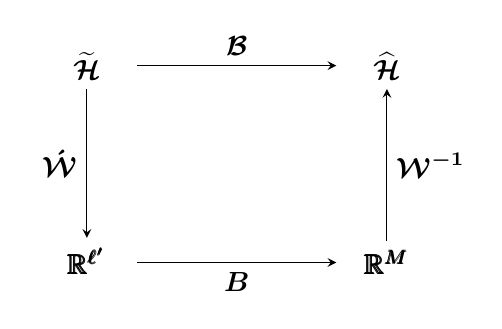
\begin{tikzpicture}
  \matrix (m) [ampersand replacement=\&, matrix of math nodes, 
                 row sep=0.75in,column sep=1in,minimum width=0.5in] {
     \boldsymbol\fspaceD \& \boldsymbol\fspaceApprox \\
     \pmb{\R^{\ncontrol}} \& \pmb{\R^{\ncent}} \\};
  \path[-stealth]
    (m-1-1) edge node [left] {$\boldsymbol\weightmapC$} (m-2-1)
            edge [right] node [above] {$\boldsymbol\controlop$} (m-1-2)
    (m-2-1.east|-m-2-2) edge node [below] {$\boldsymbol B$} node [above] {} (m-2-2)
    (m-2-2) edge node [right] {$\boldsymbol\weightmapI$} (m-1-2);            
\end{tikzpicture}
%}% end resize box
}% end subfloat
\caption{Commutative diagrams between primal and dual spaces}
\vspace{-0.2in}
\label{fig:commute_sysop}
\end{figure}
%\end{enumerate}
In the approximate space case, we replace the transition operator $\sysop:\fspace\to\fspace$ in \eqref{ideal_lin_evol} by $\sysopApprox:\fspaceApprox\to\fspaceApprox$.
This approximate regime, which combines the flexibility of a truly nonparametric approach with computational realizability, still allows for the representation of rich phenomena, as will be seen in the sequel, and in Figure \ref{fig:kernel_variation}. 
The finite-dimensional evolution equations approximating \eqref{ideal_lin_evol} in dual form are
\vspace{-0.05in}
\begin{align} \eqlabel{k_measure}
 \weight_{\tindex+1} = \dualopApprox\weight_{\tindex} + \processnoise_{\tindex}, \quad 
 \meas_{\tindex} = \obsMat \weight_{\tindex} +\measnoise_{\tindex},
\end{align}
where we have matrices $\dualopApprox\in \R^{\ncent\times\ncent}, \ \obsMat\in \R^{\nsamp\times\ncent}$, the vectors $\weight_{\tindex}\in\R^{\ncent}$, and where we have slightly abused notation to let $\meas_{\tindex}, \processnoise_{\tindex}$ and $\measnoise_{\tindex}$ denote their $\fspaceApprox$ counterparts. Here $\obsMat$ is the matrix whose rows are of the form $\obsMat_{(i)} = \obsMatRow(x_i) =
 \left[\begin{smallmatrix}
  \fmapApprox_1(x_i) & \fmapApprox_2(x_i) & \cdots & \fmapApprox_{\ncent}(x_i)
 \end{smallmatrix}\right]$. In systems-theoretic language, each row of $\obsMat$ corresponds to a \emph{measurement} at a particular location, and the matrix itself acts as a measurement operator. 

The equations \eqref{ideal_lin_evol} suggest an immediate extension to functional control problems. 
Pick another basis for $\fspace$ as $\cbasis(x) := \begin{bmatrix}\cbasis_1(x) &\cdots & \cbasis_{\ncontrol}(x)
\end{bmatrix}^T$, where the functions $\cbasis_j(x)$ are used to approximate the RKHS $\fspace$ generated by the kernel. We denote the span of these functions as $\fspaceD$. In the dictionary of atoms case, an example would be another set of atoms
 $\AtomsControl = \begin{bmatrix}\fmap(d_1) &\cdots & \fmap(d_{\ncontrol})
\end{bmatrix}$, $\fmap(d_j)\in\fspace$, $d_j\in\dom$, with $\fspaceD$ being a strict subspace of the RKHS $\fspace$  generated by the kernel. 
The functional evolution equation is then as follows:
\begin{align}\eqlabel{ideal_lin_evol_control}
 f_{\tindex+1} = \sysop f_{\tindex} + \controlop \control_{\tindex} + \eta_{\tindex}, \quad y_{\tindex} = \measop_{\tindex} f_{\tindex} + \zeta_{\tindex},
\end{align}
where the control functions $\control_{\tindex}$ evolve in $\fspaceD$, and $\controlop:\fspaceD\to\fspaceApprox$. To derive the finite-dimensional equivalent of $\controlop$, we have to work out the structure of the matrix $B$: since $\fspaceApprox$ is not, in general, isomorphic to $\fspaceD$, this imposes strict restrictions on $B$. We can derive $B$ using least squares using the inner product of $\fspace$. An instructive example is where both $\fspaceApprox$ and $\fspaceD$ are generated by dictionaries of atoms; recall that in this case, $\Atoms = 
 \begin{bmatrix}\fmap(c_1) &\cdots & \fmap(c_{\ncent})
\end{bmatrix}$ is the basis for $\fspaceApprox$, and let $\control = \sum_{j=1}^{\ncontrol}\weightc_j\fmap(d_j)$, and let $\Atoms = 
 \begin{bmatrix}\fmap(c_1) &\cdots & \fmap(c_{\ncent})
\end{bmatrix}$ be the basis for $\fspaceC$. Then the projection of $\delta$ onto $\fspaceApprox$ can be derived as 
%\begin{align*}
%\vspace{0.1in}
\resizebox{1.0\columnwidth}{!}{ 
 $\begin{bmatrix}
  \l \delta, \fmap(c_1) \r_{\fspace}\\
   \vdots\\
  \l \delta, \fmap(c_{\ncent}) \r_{\fspace} 
 \end{bmatrix}
 = 
 \underbrace{
 \begin{bmatrix}
  \Kiprod{d_1}{c_1} & \cdots & \Kiprod{d_{\ncontrol}}{c_1}\\
   \vdots  &\ddots &\vdots\\
  \Kiprod{d_1}{c_{\ncent}} & \cdots & \Kiprod{d_{\ncontrol}}{c_{\ncent}}
 \end{bmatrix}}_{\empKCD}
  \begin{bmatrix}
   \weightc_1\\
   \vdots\\
   \weightc_{\ncontrol}
  \end{bmatrix}.$
}
%\end{align*}
Note that in the dictionary of atoms case, the entries of $\empKCD$ can be computed in closed form as ${\empKCD}_{ij}:= \kernel(d_i, c_j)$,
using the reproducing property. 
This derivation shows that the operator $B$ is simply $\empKCD\in\R^{\ncent\times\ncontrol}$, the kernel matrix between the data $\centers$ generating the atoms $\Atoms$ of $\fspaceApprox$ and the data $\centerscontrol$ generating the atoms $\AtomsControl$ of $\fspaceD$. 
% Using similar arguments, it can be shown that, given sensing locations $\data = \{x_1,x_2,\dots, x_{\nsamp}\}$, $\empKD\in\R^{\nsamp\times\ncontrol}$ is the kernel matrix between $\data$ and $\centerscontrol$. 
Thus, the finite-dimensional evolution equations equivalent to \eqref{ideal_lin_evol_control} are
\begin{align}
 \weight_{\tindex} = \dualopApprox\weight_{\tindex} + \empKCD\weightc_{\tindex}, \quad
 y_{\tindex} = \empK_{\tindex} w_{\tindex} \eqlabel{k_measure_c1}.
\end{align}
We define the \emph{generalized observability matrix} \cite{zhou:bk:96} as 
%\begin{align}\eqlabel{obs_mat}
$  \Obs_{\Tset} = 
 \left[
 \begin{smallmatrix}
  \empK \dualopApprox^{\tindex_1}\\
  \cdots\\
  \empK \dualopApprox^{\tindex_\otime}
 \end{smallmatrix}
 \right] $
%\end{align}
where $\Tset = \{\tindex_1, \dots, \tindex_{\otime}\}$ are the set of instances $\tindex_i$
when we apply the operator $\empK$. A linear system is said to be \emph{observable} if $\Obs_{\Tset}$ has full column rank (i.e. $\mathrm{Rank} (\Obs_{\Tset})=\ncent$) for 
$\Tset = \{0, 1, \dots, \ncent-1\}$ \cite{zhou:bk:96}. Observability guarantees two critical facts: firstly, it guarantees that the state $\weight_0$ can be recovered exactly from a finite series of measurements $\{y_{{\tindex}_1}, y_{{\tindex}_2}, \dots, y_{{\tindex}_{\otime}}\}$; in particular, defining $y_{\Tset} = \begin{bmatrix}y_{{\tindex}_1}^T, y_{{\tindex}_2}^T, \cdots, y_{{\tindex}_{\otime}^T}\end{bmatrix}^T$, we have that $y_{\Tset} = \Obs_{\Tset}\weight_0.$  Secondly, it guarantees that a feedback based \emph{observer} can be designed such that the estimate of $\weight_{\tindex}$, denoted by $\estweight_{\tindex}$, converges exponentially fast to $\weight_{\tindex}$ in the limit of samples. Note that all our theoretical results assume $\dualopApprox$ is available: while we perform system identification in the experiments (\cite{Kingravi16_NIPS}), it is not the focus of the paper. 

We are now in a position to formally state the spatiotemporal modeling, control, and inference problems being considered: given a spatiotemporally evolving system modeled using \eqref{k_measure}, choose a set of $\nsamp$ sensing locations such that even with $\nsamp\ll \ncent$, the functional evolution of the spatiotemporal model can be estimated (which corresponds to \emph{monitoring}), can be predicted robustly (which corresponds to \emph{Bayesian filtering}), and which can be controlled (which corresponds to \emph{functional control}). Our approach to solve the monitoring and prediction problem relies on the design of the measurement operator $\empK$ so that the pair $(\empK, \dualopApprox)$ is observable: any Bayesian state estimator (e.g. a Kalman filter) utilizing this pair is denoted as a \textbf{kernel observer} \footnote{In the case where no measurements are taken, for the sake of consistency, we denote the state estimator as an \textbf{autonomous kernel observer}, despite this being somewhat of an oxymoron.}. In the controls case, given a spatiotemporally evolving system modeled using \eqref{k_measure_c1}, we need to choose a set of $\nsamp$ sensing locations and $\ncontrol$ control locations, such that even with $\nsamp\ll \ncent, \ \ncontrol \ll\ncent$, the functional evolution of the spatiotemporal model can be controlled; in this case, we must design both a measurement operator $\empK$ and a control operator $\empKCD$ such that the pair $(\empKCD, \dualopApprox)$ is controllable: a controls system utilizing this pair and the measurement operator $\empK$ is denoted as a \textbf{kernel controller}.

\subsection{Preliminaries on Rational Canonical Structures}\label{sec_prelim}
We take a geometric approach towards the choice of sampling locations for inferring $\weight_{\tindex}$ in  \eqref{k_measure}; the extension for control is similar.  We use the notation $\linspace$, with $\dims(\linspace)=\ncent$, to emphasize the fact that these theorems hold for any finite-dimensional vector space. Consider the linear operator $\sysop:\linspace\rightarrow\linspace$, and recall that the definition of observability requires the construction of a linear operator $\measop:\linspace\to\linspaceout$, with $\dim(\linspaceout) = \nsamp$, such that 
$\Rank\left[
 \begin{smallmatrix}
  \left(\measop\right)^T &
  \cdots &
  \left(\measop \sysop^{\ncent-1}\right)^T
 \end{smallmatrix}
 \right]^T = \ncent$. 
In most applications, if $\nsamp\geq\ncent$, and $\Rank\measop = \nsamp$, it is reasonable to expect that observability may be achieved. However, for our purposes, $\nsamp$ must be \emph{significantly} less than $\ncent$. Therefore, we must design $\measop$ with as small a rank as possible. To do so, we require a series of vectors $\linvec_i$ that, under repeated iterations of $\sysop$, can generate a basis for $\linspace$. For this task, we will use a fundamental decomposition result from the theory of modules, known as the \emph{rational canonical structure} of $\sysop$ \cite{wonham1974linear}. The intuition here is that if the sequence $\{\linvec_i\}_{i}$ can generate this basis, it can be directly used to construct $\measop$.

The linear operator $\sysop:\linspace\rightarrow\linspace$ has a characteristic polynomial $\charpoly(\eval) $ such that $\charpoly(\sysop)=0 $ by the Cayley-Hamilton theorem. The minimal polynomial (MP) of $\sysop$ is the monic polynomial $\minpoly(\cdot)$ of least degree (denoted by $\degs(\cdot)$) given as 
$\minpoly(\eval) = \polycoeff_0 + \polycoeff_1\eval +\cdots + \eval^{\degs(\minpoly)} = 0$, such that
$\minpoly(\sysop)=\polycoeff_0 I + \polycoeff_1\sysop +\cdots + \sysop^{\degs(\minpoly)} = \bm{0}$. 
The MP is unique and divides $\charpoly(\lambda)$, so that $ \degs(\minpoly) \leq \degs(\charpoly)$. The MP of a vector $\linvec\in\linspace$ \emph{relative to $\sysop$} is the unique monic polynomial $\minpolyv_{\linvec}$ of least degree such that 
$\minpolyv_{\linvec}(\sysop)\linvec= \polycoeff_0\linvec + \polycoeff_1\sysop\linvec + \cdots + \sysop^{\degs(\minpoly)}\linvec = 0$. 
If $\degs(\alpha) = \ncent$, then $\sysop$ is \emph{cyclic} and $\exists\linvec\in \linspace$, such that the vectors $\{\linvec, \sysop \linvec,\dots,\sysop^{\ncent-1}\linvec\}$ form a basis for $\linspace$; this is the same as saying that the pair $(\linvec^T,\sysop^T)$ is observable.    
A subspace $\subspace\subset\linspace$ s.t. $\sysop\subspace\subset\subspace$ is \emph{$\sysop$-cyclic} if  $\restrict{\sysop}{\subspace}$, the restriction of $\sysop$ to the subspace $\subspace$, is cyclic. If $\minpoly(\eval)$ is the minimal polynomial of $\sysop$ and $\degs(\minpoly) = \acycdeg < \ncent$, $\exists~\linvec\in\linspace$ such that $\{\linvec, \sysop \linvec,\dots,\sysop^{\acycdeg-1}\linvec\}$ span an $\acycdeg$-dimensional $\sysop$-cyclic subspace $\subspace$, with $\linvec$ being the \emph{cyclic generator} of $\subspace$.  The subspace $\subspace$ decomposes $\linspace$ relative to $\sysop$. By the rational canonical structure theorem (Theorem 0.1 of \cite{wonham1974linear}), $\sysop$ can be successively decomposed into subspaces $\linspace_i \subset \linspace$, $i\in \{1,\dots,\minmeas\}$, s.t. $\linspace = \linspace_1 \oplus ... \oplus \linspace_{\minmeas}$, $\sysop\linspace_i \subset \linspace_i$, and  $\sysop_{|\linspace_i}, i \in \{1,\dots,\minmeas\}$, are cyclic\footnote{In general, the subspaces $\linspace_i$ are not unique for a fixed $\sysop$.}. The integer $\minmeas$ is unique and is called the \emph{cyclic index of $\sysop$}. 

One of our main results is to show that the cyclic index is a lower bound on the number of measurements required to reconstruct $\weight_{\tindex}$ (see Prop. \ref{prop:3} and Alg. 1 in \cite{Kingravi16_NIPS}). The matrix transform associated to this theorem is known as the \emph{Frobenius normal form} (denoted by $\FrobC\in\R^{\ncent\times\ncent}$ ): for $\sysop\in\R^{\ncent\times\ncent}$,  $\exists \FrobP\in\R^{\ncent\times\ncent}$ invertible  such that $\sysop = \FrobP\FrobC\FrobP^{-1}$. We will also use the \emph{Jordan decomposition}, where for $\sysop\in\R^{\ncent\times\ncent}$, $\exists \JorP\in\R^{\ncent\times\ncent}$ invertible such that $\sysop = \JorP\JorLa \JorP^{-1}$, where $\JorLa$ is a unique block diagonal matrix with Jordan blocks with $\eval_i$ along the diagonal. 
If all the eigenvalues $\eval_i$ are nonzero and real, we say the matrix has a \emph{full-rank Jordan decomposition}. 


\vspace{-0.1in}
\subsection{Main Results}\label{sec:theory_results}
%\vspace{-0.1in}
In this section, we prove results concerning the observability of spatiotemporally varying functions modeled by the functional evolution and measurement equations \eqref{k_measure} formulated in Section \ref{sec:formulation}. In particular,  observability of the system states implies that we can recover the current state of the spatiotemporally varying function using a small number of sampling locations $\nsamp$, which allows us to 1) track the function, and 2) predict its evolution forward in time. We work with the approximation $\fspaceApprox\approx\fspace$: given $\ncent$ basis functions, this implies that the dual space of $\fspaceApprox$ is $\R^{\ncent}$.
Proposition \ref{prop:1} shows that if $\dualopApprox$ has a full-rank Jordan decomposition, the observation matrix $\obsMat$ meeting a condition called \emph{shadedness} (Definition \ref{def:shaded}) is sufficient for the system to be observable. Proposition \ref{prop:2} provides a lower bound on the number of sampling locations required for observability which holds for any $\dualopApprox$.  Proposition \ref{prop:3} constructively shows the existence of an abstract measurement map $\measmap$ achieving this lower bound. Since the measurement map does not have the structure of a kernel matrix, a slightly weaker sufficient condition for the observability of any $\dualopApprox$ is in Theorem \ref{thm:1}. Finally, since both $\empK$ and $\empKCD$ are kernel matrices generated from a shared kernel, these observability results translate directly into controllability results. Proofs of all claims are in the appendix. 

\begin{definition}\label{def:shaded}
\textbf{(Shaded Observation Matrix)} Given $\kernel:\dom\times\dom\to\R$ positive-definite on a domain $\dom$, let $\{\fmapApprox_1(x), \dots, \fmapApprox_{\ncent}(x)\}$ be the set of bases generating an approximate feature map $\fmapApprox:\dom\to\fspaceApprox$, and let
$\sampSet = \sampSetLong$ be the set of sampling (or sensing) locations, with each $x_i\in\dom$. 
Let $\obsMat\in\R^{\nsamp\times\ncent}$ be the observation matrix, where $ \obsMat_{ij} := \fmapApprox_j(x_i)$. For each
row $\obsMat_{(i)} := \left[\begin{smallmatrix}
  \fmapApprox_1(x_i) & \cdots & \fmapApprox_{\ncent}(x_i)
 \end{smallmatrix}\right]$, define the set 
$\Ind_{(i)} := \{\iota_1^{(i)},\iota_2^{(i)},\dots, \iota_{\ncent_i}^{(i)}\}$ to be the indices in the observation
matrix row $i$ which are nonzero. 
Then if 
%\begin{align}\eqlabel{shaded_cond}
$\bigcup_{i\in\{1,\dots,\nsamp\}} \Ind^{(i)} = \{1,2,\dots, \ncent\}$,
%\end{align}
we denote $\obsMat$ as a \emph{shaded observation matrix} (see Figure \ref{fig:shadeda}).
\end{definition}
This definition seems quite abstract, so the following remark considers a more concrete example.
\begin{remark}\label{rem:shaded}
 let $\fmapApprox$ be generated by the dictionary given by $\shCent = \shCentLong$, $c_i\in\dom$. Note that since $\fmapApprox_j(x_i) = \l\fmap(x_i), \fmap(c_j)\r_{\fspace} = \kernel(x_i,c_j)$, $\obsMat$ is the kernel matrix between $\sampSet$ and $\shCent$. For the kernel matrix to be shaded thus implies that there does not exist an atom $\fmap(c_j)$ such that the projections $\l\fmap(x_i),\fmap(c_j)\r_{\fspace}$ vanish for all $x_i$, $1\leq i\leq \nsamp$. Intuitively, the shadedness property requires that the sensor locations $x_i$ are privy to information propagating from every $c_j$. As an example, note that, in principle, for the Gaussian kernel, a single row generates a shaded kernel matrix\footnote{However, in this case, the matrix can have many entries that are extremely close to zero, and will probably be very ill-conditioned.}.  
\end{remark}
% With this definition in place, we can prove the following proposition, which shows that if $\dualopC$ has a full-rank Jordan decomposition, a shaded observationrf matrix is sufficient to guarantee observability. 
\begin{proposition}\label{prop:1}
Given $\kernel:\dom\times\dom\to\R$ positive-definite on a domain $\dom$, let $\{\fmapApprox_1(x), \dots, \fmapApprox_{\ncent}(x)\}$ be the set of bases generating an approximate feature map $\fmapApprox:\dom\to\fspaceApprox$, and let
$\sampSet = \sampSetLong$, $x_i\in\dom$. Consider the discrete linear system on $\fspaceApprox$ given by the evolution and measurement equations \eqref{k_measure}. Suppose that a full-rank Jordan decomposition of $\dualopApprox\in\R^{\ncent\times\ncent}$ of the form $\dualopApprox = \JorP\JorLa\JorP^{-1}$ exists, where $\JorLa = 
\left[\begin{smallmatrix}\JorLa_1 &\cdots & \JorLa_{\JorMul}\end{smallmatrix}\right]$,
and there are no repeated eigenvalues. Then, given a set of time instances  $\Tset = \{\tindex_1,\tindex_2,\dots,\tindex_{\otime}\}$, and a set of sampling locations $\sampSet=\sampSetLong$,
the system \eqref{k_measure} is observable if the observation matrix $\empK_{ij}$ is shaded according to Definition \ref{def:shaded},
% $\empK^D$, the row vector generated by summing the rows of $\empK$, has all nonzero entries, 
$\Tset$ has distinct values, and $|\Tset| \geq \ncent$.
\end{proposition}
% \begin{remark}
%  For the system corresponding to \ref{prop:1}, 
% \end{remark}
When the eigenvalues of the system matrix are repeated, it is not enough for $\empK$ to be shaded. 
% Intuitively, repeated eigenvalues correspond to coupled evolution\footnote{We use the term coupled evolution to denote dynamic evolution in which some eigen-modes evolve together \gXX{check rewrite}}, which requires an increased number of sensors to discern \gXX{what's the best way to explain this better? Without invariant subspaces it may not be clear to some why this matters, should we merge this with the discussion after the below prop?}. 
In the next proposition, we take a geometric approach and utilize the rational canonical form  of $\dualopApprox$ to obtain a lower bound on the number of sampling locations required. Let $\nevals$ be the number of unique eigenvalues of $\dualopApprox$, and let $\geomMult{\eval_i}$ denote the geometric multiplicity of eigenvalue $\eval_i$. Then the \emph{cyclic index} of $\dualopApprox$ is defined as $\minmeas = \max_{1\leq i\leq\nevals}{\geomMult{\eval_i}}$\cite{wonham1974linear} (see preliminary section \ref{sec_prelim} for details).
\begin{proposition}\label{prop:2}
 Suppose that the conditions in Proposition \ref{prop:1} hold, with the relaxation that
 the Jordan blocks $\left[\begin{smallmatrix}
                           \JorLa_1 &\cdots & \JorLa_{\JorMul}
                          \end{smallmatrix}\right]$ may have 
 repeated eigenvalues (i.e. $\exists \JorLa_i$ and $\JorLa_j$ s.t. $\eval_i = \eval_j$). 
 Then there exist kernels $\kernel(x,y)$ such that 
 the lower bound $\minmeas$ on the number of sampling locations $\nsamp$ is given by the cyclic index of $\dualopApprox$. In other words, the system in \eqref{k_measure} is observable if $ \nsamp \geq \ell$.
\end{proposition}
Section \ref{sec:discussion} gives a concrete example to build intuition regarding this lower bound. We now show how to construct a matrix $\measmap$ corresponding to the lower bound $\minmeas$.
% \begin{figure}[t!]
% 	\begin{algorithm}[H]
% 		\caption{Measurement Map $\measmap$}
% 		\label{alg:measmap}
% 		\begin{algorithmic}
% 			\begin{footnotesize} 
% 				\STATE {\bfseries Input:} $\dualopApprox\in\R^{\ncent\times\ncent}$
% 				\STATE Compute Rational canonical form, such that $ \FrobC  = \FrobP^{-1} \dualopApprox^T\FrobP$. Set $\FrobC_0:=\FrobC$, and
% 				$\ncent_0:=\ncent$. 
% 				%           Obtain subspaces 
% 				%           $\linspace_i\subset\R^{\ncent}$ s.t. $\R^{\ncent} = \linspace_1\oplus\cdots\oplus\linspace_{\minmeas}$.
% 				\FOR{$i=1$ {\bfseries to} $\minmeas$}
% 				\STATE Obtain MP $\minpoly_i(\eval)$ of $\FrobC_{i-1}$. 
% 				This returns associated indices $\mmapInd{i}\subset\{1,2,\dots,\ncent_{i-1}\}$. 
% 				%             \STATE Use $\mmapInd{i}$ to select submatrix $\widetilde{\FrobP}_i$, where an index $j\in\mmapInd{i}$ 
% 				%                    indicates selection of the row and column associated to $j$.
% 				\STATE Construct vector $\linvec_i \in \R^{\ncent}$ such that 
% 				$\minpolyv_{\linvec_i}(\eval)=\minpoly_{i}(\eval)$ .
% 				\STATE Use indices $\{1,2,\dots,\ncent_{i-1}\}\setminus\mmapInd{i}$ to select matrix $\FrobC_i$. Set 
% 				$\ncent_i:= |\{1,2,\dots,\ncent_{i-1}\}\setminus\mmapInd{i}|$
% 				\ENDFOR
% 				\STATE Compute $ \premeasmap = [\linvec_1^T, \linvec_2^T,...,\linvec_{\minmeas}^T]^T$
% 				\STATE {\bfseries Output:} $ \measmap =\premeasmap\FrobP^{-1}  $
% 			\end{footnotesize}
% 		\end{algorithmic}
% 	\end{algorithm} 
% 	\vspace{-0.2in}
% \end{figure}
\begin{proposition}\label{prop:3}
Given the conditions stated in Proposition \ref{prop:2}, it is possible to construct a measurement map $\measmap \in \R^{\minmeas\times\ncent}$ for the system given by \eqref{k_measure}, such that the pair $(\measmap, \dualopApprox)$ is observable.
\end{proposition}
The construction provided in the proof of Proposition \ref{prop:3} is utilized in Algorithm \ref{alg:measmap}, which uses the rational canonical structure of $\dualopApprox$ to generate a series of vectors $\linvec_i\in\R^{\ncent}$, whose iterations $\{\linvec_1,\dots,\dualopApprox^{\acycdeg_1-1}\linvec_1,\dots,\linvec_{\minmeas},\dots,\dualopApprox^{\acycdeg_{\minmeas}-1}\linvec_{\minmeas}\}$ generate a basis for $\R^{\ncent}$.
Unfortunately, the measurement map $\measmap$, being an abstract construction unrelated to the kernel, does not directly select $\sampSet$. We will show how to use the measurement map to guide a search for $\sampSet$ in Remark \ref{rem:1} (in Appendix). For now, we state a sufficient condition for observability of a general system. 
\begin{theorem}\label{thm:1}
 Suppose that the conditions in Proposition \ref{prop:1} hold, with the relaxation that
 the Jordan blocks $\begin{bmatrix}\JorLa_1 & &\cdots & \JorLa_{\JorMul}\end{bmatrix}$ may have 
 repeated eigenvalues. Let $\minmeas$ be the cyclic index of $\dualopApprox$.
 Define 
 \begin{align}\eqlabel{empKShadFull}
  \empKShadFull = \left[\begin{smallmatrix}
                    \empK^{{(1)}^T} & 
                    \cdots &
                    \empK^{{(\minmeas)}^T}
                  \end{smallmatrix}\right]^T
 \end{align}
 as the \emph{$\minmeas$-shaded matrix} (see Figure \ref{fig:shadedb}) which consists of $\minmeas$ shaded matrices with the property that any subset of
 $\minmeas$
 columns in the matrix are linearly independent from each
 other. Then system \eqref{k_measure} is observable if $\Tset$ has distinct values, and $|\Tset| \geq \ncent$.
\end{theorem}
While Theorem \ref{thm:1} is a quite general result, the condition that any $\minmeas$ columns of $\empKShadFull$ be linearly independent is a very stringent condition. 
One scenario where this condition can be met with minimal measurements is in the case when the feature map $\fmapApprox(x)$ is generated by a dictionary of atoms with the Gaussian RBF kernel evaluated at sampling locations $\sampSetLong$ according to \eqref{fmap_dict}, where $x_i\in\dom\subset\R^d$, and $x_i$ are sampled from a non-degenerate probability distribution on $\dom$ such as the uniform distribution. For a semi-deterministic approach, when the dynamics matrix $\dualopApprox$ is block-diagonal, we can utilize a simple heuristic:
\begin{remark}\label{rem:1}
 Let $\dom$ be compact, $\shCent = \shCentLong$, $c_i\in\dom$, and let the approximate feature map be defined by \eqref{fmap_dict}. Consider the system \eqref{k_measure} with $\dualopApprox=\JorLa$, and let $\Tset = \{0,1,\dots,\ncent-1\}$. Then the measurement map $\measmap$'s values lie in $\{0, 1\}$; in particular, each row $\measmap^{(j)}$, $j\in\{1,\dots,\minmeas\}$, corresponds to a subspace $\fsubspaceC{j}$, generated by a subset of centers $\shCent^{(j)}\subset\shCent$. Generate samples $x_i^{(j)}$ to create a kernel matrix $\empK^{(j)}$ that is shaded only with respect to centers $\shCent^{(j)}$. Once this is done, move on to the next subspace $\fsubspaceC{j+1}$. When all $\minmeas$ rows of $\measmap$ are accounted for, construct the matrix $\empKShadFull$ as in \eqref{empKShadFull}. Then the resulting system $(\empKShadFull, \dualopApprox)$ is observable. 
\end{remark}

%\begin{figure}
%\begin{algorithm}[H]
%\caption{Measurement Map $\measmap$}
%\label{alg:measmap}
%\begin{algorithmic}
% \begin{footnotesize} 
%   \STATE {\bfseries Input:} $\dualopApprox\in\R^{\ncent\times\ncent}$
%   \STATE Compute Jordan canonical form, such that $ \JorLa  = \JorP^{-1} \dualopApprox^T\JorP$. Set $\JorLa_0:=\JorLa$, and
%          $\ncent_0:=\ncent$. 
%          \FOR{$i=1$ {\bfseries to} $\minmeas$}
%            \STATE Obtain MP $\minpoly_i(\eval)$ of $\JorLa_{i-1}$. 
%                   This returns associated indices $\mmapInd{i}\subset\{1,2,\dots,\ncent_{i-1}\}$. 
%            \STATE Construct vector $\linvec_i \in \R^{\ncent}$ such that 
%                   $\minpolyv_{\linvec_i}(\eval)=\minpoly_{i}(\eval)$ .
%            \STATE Use indices $\{1,2,\dots,\ncent_{i-1}\}\setminus\mmapInd{i}$ to select matrix $\JorLa_i$. Set 
%                   $\ncent_i:= |\{1,2,\dots,\ncent_{i-1}\}\setminus\mmapInd{i}|$
%          \ENDFOR
%   \STATE Compute $ \premeasmap = [\linvec_1, \linvec_2,...,\linvec_{\minmeas}]^T$
%   \STATE {\bfseries Output:} $ \measmap =\premeasmap\JorP^{-1}  $
%\end{footnotesize}
%\end{algorithmic}
%\end{algorithm}
%\vspace{-0.2in} 
%\end{figure}
This heuristic is formalized in Algorithm 2 in the supplementary. Note that in practice, the matrix $\dualopApprox$ needs to be inferred from measurements of the process $f_{\tindex}$. If no assumptions are placed on $\dualopApprox$, it's clear that at least $\ncent$ sensors are required for the system identification phase. Future work will study the precise conditions under which system identification is possible with less than $\ncent$ sensors. 
\begin{figure*}[ht!]
\centering
\resizebox{1\textwidth}{!}{
\framebox[1.1\textwidth]{
 \begin{tikzpicture}[->,>=stealth',auto,node distance=1cm,
  thick,main node/.style={circle,draw,font=\sffamily\Large\bfseries}]
  \node[inner sep=0pt,label=below:{\tiny Physical 
                                  sampling locations},draw] (physical) at (-8,-0.3)
    {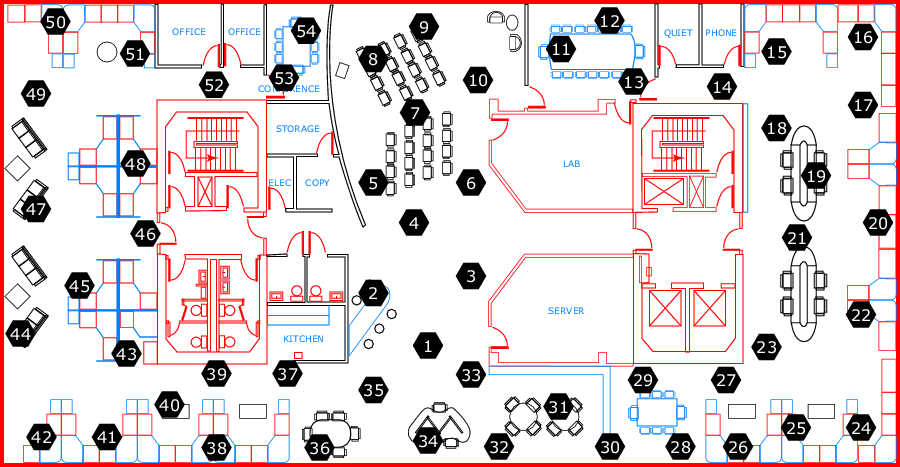
\includegraphics[width=0.13\textwidth,
                      height=0.08\textwidth]{figures/lab.png}};
  \node[inner sep=0pt,label=below:{\tiny Data locations},draw] (data) at (-4.25,-0.3)
    {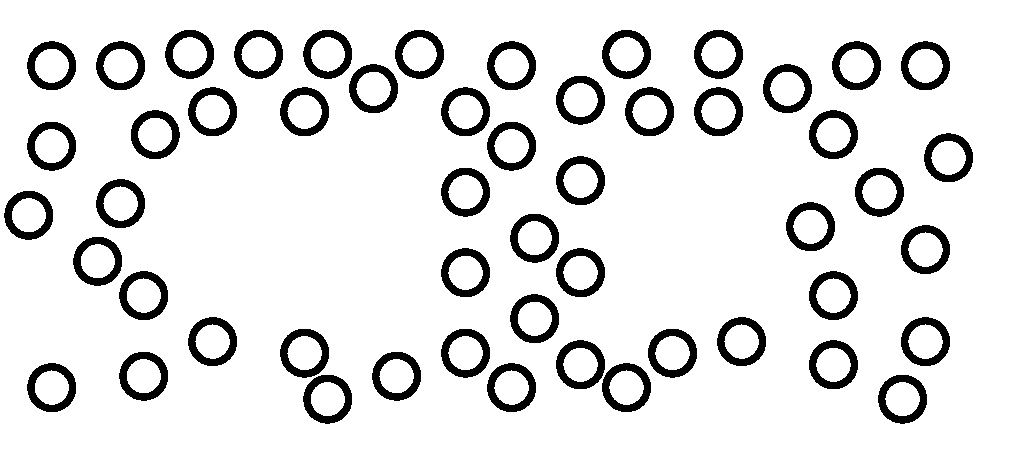
\includegraphics[width=0.13\textwidth,
                      height=0.08\textwidth]{figures/locations.pdf}};
  \node[inner sep=0pt,label=below:{\tiny Functional inference 
                                   (for $\estsysop$)},draw] (inference) at (-0.5,-0.3)
    {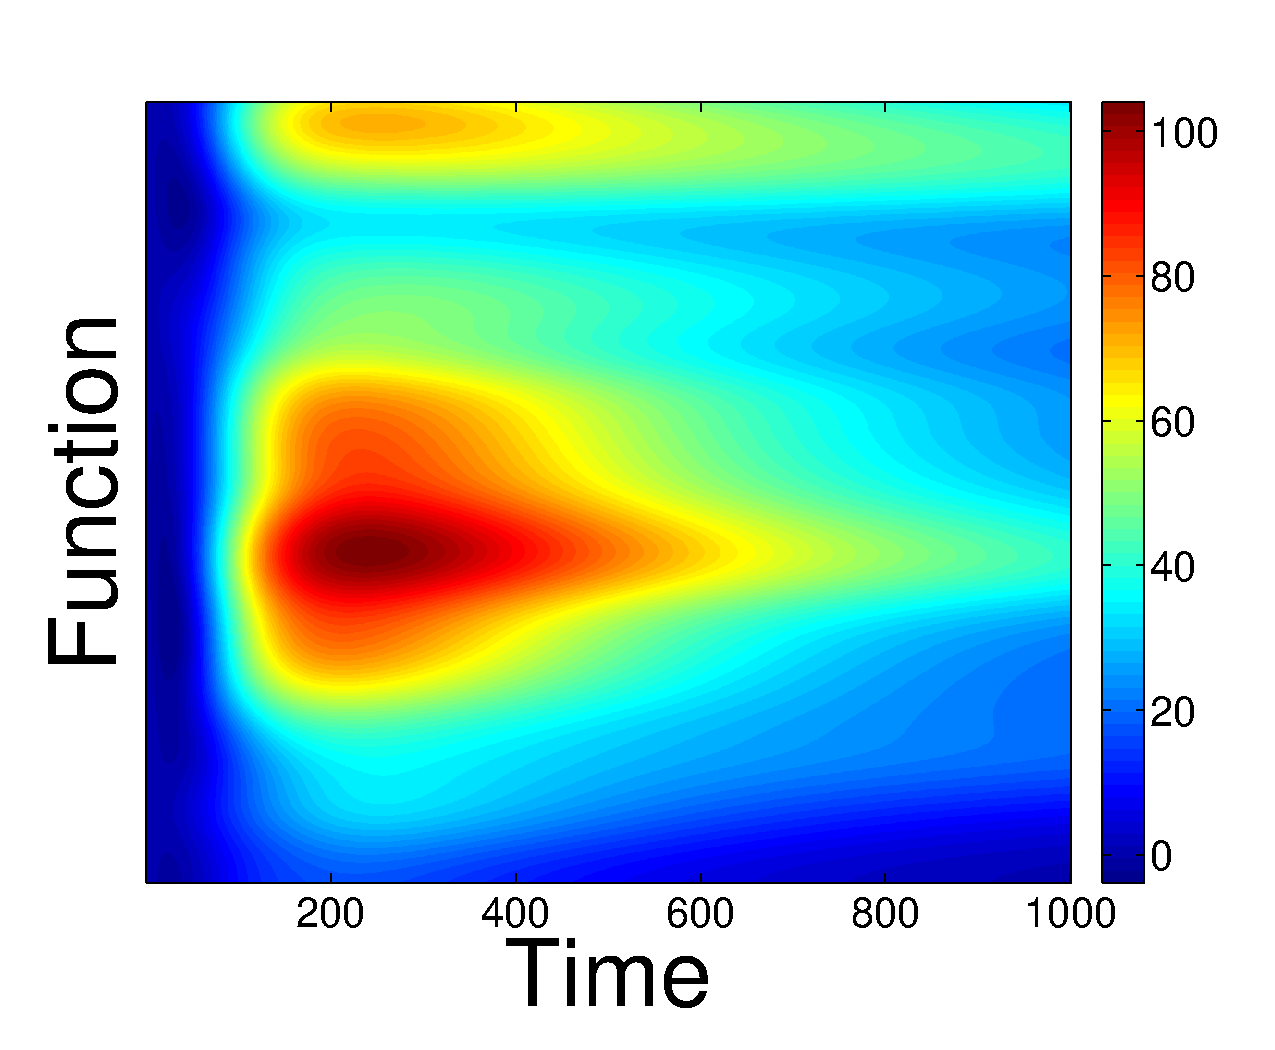
\includegraphics[trim=2.4cm 2.6cm 3.4cm 1.5cm,clip,
                      width=0.13\textwidth,
                      height=0.08\textwidth]{figures/kernel_evol_cauchy.pdf}};    
  \node[inner sep=0pt,label={[align=center]
       below:{\tiny Sensor location selection after\\[-1.7\jot]
              \tiny basis decomposition ($\minmeas=3$)}},draw] 
       (sensors) at (3.25,-0.3)
       {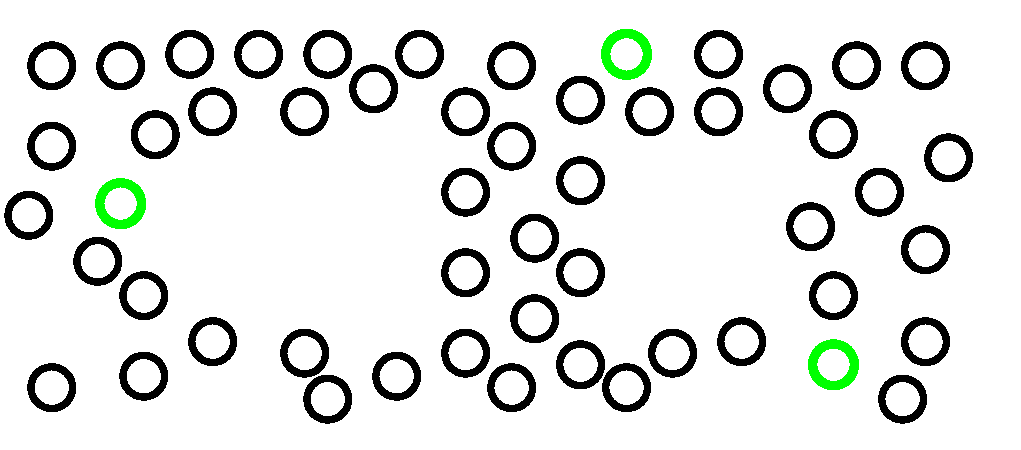
\includegraphics[width=0.13\textwidth,
                         height=0.08\textwidth]{figures/locations_sensors.pdf}};                          
  \node[inner sep=0pt,label=below:{\tiny Physical sensor placement},draw] (placement) at (6.75,-0.3)
    {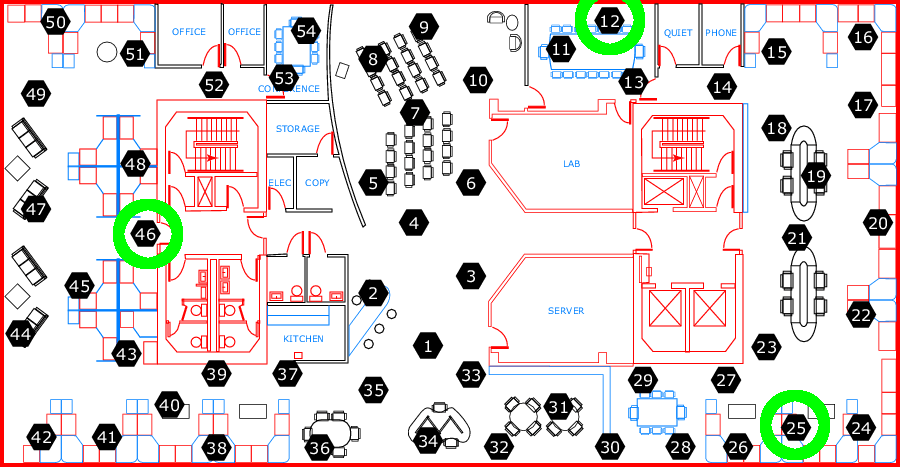
\includegraphics[width=0.13\textwidth,
                      height=0.08\textwidth]{figures/lab_sensors2.png}};                                                
  \path[every node/.style={font=\sffamily\small}]
    (physical) edge node [right] {} (data)
    (data) edge node [right] {} (inference)
    (inference) edge node [right] {} (sensors)
    (sensors) edge node [right] {} (placement);
\end{tikzpicture}
} % end framebox
} % end resizebox
\caption{
Overall description of how the kernel observer fits in the sensing framework. Physical 
locations are mapped to data locations, over which historical data is collected 
as a time series. Functional inference is performed over $\fspaceApprox$ to 
solve for $\estsysop$. The measurement operator $\empK$ is then computed 
(see Figure \ref{fig:sensplace}), leading to sensor placement. 
}\label{fig:overall_system}
\end{figure*}
\begin{figure*}[ht!]
  \begin{minipage}{\textwidth}
  \centering
  \begin{minipage}{0.47\textwidth}
  \resizebox{1\textwidth}{!}{
  \framebox[1.2\textwidth]{  
  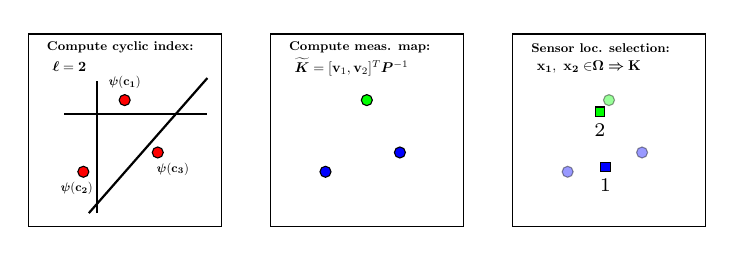
\begin{tikzpicture}[scale=1.0, every node/.style={minimum size=1cm},on grid]    
	\begin{scope}[scale=\diagscale, xshift=-250, yshift=0]
		% The frame:
		\fill[white,fill opacity=.85] (0,0) rectangle (7,7); % Opacity
		\draw[black, thin] (0,0) rectangle (7,7); 
		 % Agents:
		\draw [fill=red]
			(4.7,2.7) circle (.2) % Firms
			(2,2) circle (.2) % Households
			(3.5,4.6) circle (.2); % Banks
		\fill[black]
			(0.5,6.5) node[right, scale=\diagtexttop] {\small \textbf{Compute cyclic index:}}
			(0.7,5.8) node[right, scale=\diagtexttop]
			{$\boldsymbol\minmeas = \mathbf{2}$}
			(4.5,2.1) node[right, scale=\diagtext]{$\boldsymbol\fmap(\mathbf{c_3})$}
			(2.5,1.4) node[left, scale=\diagtext]{$\boldsymbol\fmap(\mathbf{c_2})$}
			(3.5,4.6) node [above, scale=\diagtext] {$\boldsymbol\fmap(\mathbf{c_1})$}
			;
        % draw lines representing possible choices of decomposition                
        \draw[thick](1.3,4.1) to (6.5,4.1);
        \draw[thick](2.2,0.5) to (6.5,5.4);
        \draw[thick](2.5,0.5) to (2.5,5.3);
	\end{scope} 
	\begin{scope}[scale=\diagscale, xshift=0, yshift=0]
		% The frame:
		\draw[black, thin] (0,0) rectangle (7,7); 
		% Agents:
		\draw [fill=blue]
			(4.7,2.7) circle (.2) % Firms
			(2,2) circle (.2); % Households
		\draw [fill=green]			
			(3.5,4.6) circle (.2); % Banks
		 % Labels:
		\fill[black]
		        (0.5,6.5) node[right, scale=\diagtexttop] {\small \textbf{Compute meas. map:}}
			(0.7,5.8) node[right, scale=\diagtexttop]
			{$\boldsymbol\measmap =[\mathbf\linvec_1, 
			                        \mathbf\linvec_2]^T\boldsymbol\JorP^{-1}$}
% 			(4.5,2.1) node[right, scale=\diagtext]{$\boldsymbol\fmap(\mathbf{c_3})$}
% 			(2.5,1.4) node[left, scale=\diagtext]{$\boldsymbol\fmap(\mathbf{c_2})$}
% 			(3.5,4.6) node [above, scale=\diagtext] {$\boldsymbol\fmap(\mathbf{c_1})$}
			;
	\end{scope} 
	\begin{scope}[scale=\diagscale, xshift=250, yshift=0]
		% The frame:
		\draw[black, thin] (0,0) rectangle (7,7); 
		% Agents:
		\draw [fill=blue, opacity=0.4]
			(4.7,2.7) circle (.2) 
			(2,2) circle (.2)
			;
		\draw [fill=blue]
			(3.2,2) rectangle (3.55,2.35)
			; 
			\node (one) at (3.37,1.5) {\scriptsize$ 1 $};
		\draw [fill=green, opacity=0.4]
			(3.5,4.6) circle (.2)
			;
		\draw [fill=green]			
			(3.0,4.0) rectangle (3.35,4.35)
			;
			\node (two) at (3.17,3.5) {\scriptsize$ 2 $};
		\fill[black]
		        (0.5,6.5) node[right, scale=\diagtexttop] {\small \textbf{Sensor loc. selection:}}
			(0.7,5.8) node[right, scale=\diagtexttop]
			{$\mathbf{x_1, \ x_2\in}\boldsymbol\dom \boldsymbol\Rightarrow \empKShadFull$}
% 			(4.5,2.1) node[right, scale=\diagtext]{$\boldsymbol\fmap(\mathbf{c_3})$}
% 			(4.5,2.1) node[right, scale=\diagtext]{$\boldsymbol\fmap(\mathbf{x_2})$}
% 			(2.5,1.4) node[left, scale=\diagtext]{$\boldsymbol\fmap(\mathbf{c_2})$}
% 			(1.4,4.7) node[right, scale=\diagtext]{$\boldsymbol\fmap(\mathbf{x_1})$}
% 			(3.5,4.6) node [above, scale=\diagtext] {$\boldsymbol\fmap(\mathbf{c_1})$}
			;
	\end{scope}	
  \end{tikzpicture}
  } % end framebox
  } % end resizebox  
  \end{minipage}
  \begin{minipage}{0.47\textwidth}
  \resizebox{1\textwidth}{!}{
  \framebox[1.2\textwidth]{  
  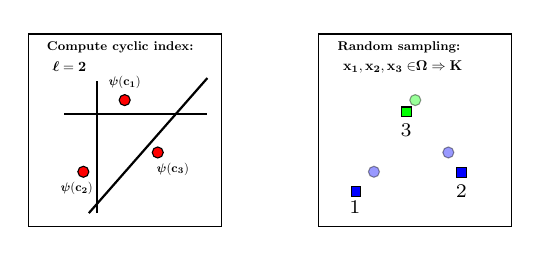
\begin{tikzpicture}[scale=1.0, every node/.style={minimum size=1cm},on grid]  
	\begin{scope}[scale=\diagscale, xshift=-150, yshift=0]
		% The frame:
		\fill[white,fill opacity=.85] (0,0) rectangle (7,7); % Opacity
		\draw[black, thin] (0,0) rectangle (7,7); 
		 % Agents:
		\draw [fill=red]
			(4.7,2.7) circle (.2) % Firms
			(2,2) circle (.2) % Households
			(3.5,4.6) circle (.2); % Banks
		\fill[black]
			(0.5,6.5) node[right, scale=\diagtexttop]{\small \textbf{Compute cyclic index:}}
			(0.7,5.8) node[right, scale=\diagtexttop]
			{$\boldsymbol\minmeas = \mathbf{2}$}
			(4.5,2.1) node[right,scale=\diagtext]{$\boldsymbol\fmap(\mathbf{c_3})$}
			(2.5,1.4) node[left,scale=\diagtext]{$\boldsymbol\fmap(\mathbf{c_2})$}
			(3.5,4.6) node [above, scale=\diagtext] {$\boldsymbol\fmap(\mathbf{c_1})$};
        % draw lines representing possible choices of decomposition                
        \draw[thick](1.3,4.1) to (6.5,4.1);
        \draw[thick](2.2,0.5) to (6.5,5.4);
        \draw[thick](2.5,0.5) to (2.5,5.3);
	\end{scope} 
	\begin{scope}[scale=\diagscale, xshift=150, yshift=0]
		% The frame:
		\draw[black, thin] (0,0) rectangle (7,7); 
		% Agents:
		\draw [fill=blue, opacity=0.4]
			(4.7,2.7) circle (.2) % Firms
			(2,2) circle (.2)
			;
		\draw [fill=blue]
			(1.17,1.1) rectangle (1.17+0.35,1.1+0.35)
			(5.0,1.8) rectangle (5.35,2.15)
                        ;
           \node (one) at (1.31,0.7) {\scriptsize$ 1 $};
           \node (two) at (5.17,1.3) {\scriptsize$ 2 $};
		\draw [fill=green, opacity=0.4]
			(3.5,4.6) circle (.2)
			;
		\draw [fill=green]
                        (3.0,4.0) rectangle (3.35,4.35)
			;
			\node (three) at (3.17,3.5) {\scriptsize$ 3 $};
		 % Labels:
		\fill[black]
		        (0.5,6.5) node[right, scale=\diagtexttop] {\small \textbf{Random sampling:}}
			(0.7,5.8) node[right, scale=\diagtexttop]
			{$\mathbf{x_1, x_2, x_3\in} \boldsymbol\dom \Rightarrow \empKShadFull$}
% 			(4.5,2.1) node[right,scale=\diagtext]{$\boldsymbol\fmap(\mathbf{c_3})$}
% 			(2.5,1.4) node[left,scale=\diagtext]{$\boldsymbol\fmap(\mathbf{c_2})$}
% 			(3.5,4.6) node [above, scale=\diagtext] {$\boldsymbol\fmap(\mathbf{c_1})$}
			;
	\end{scope} 
  \end{tikzpicture}
  } % end framebox
  } % end resizebox                      
  %\captionof{figure}{Sensor selection using random sampling} \label{fig:sselec_rand}
  \end{minipage} 
  \end{minipage} 
  \caption{
  Diagram demonstrating sensor placement using the measurement map or random sampling approaches. 
  The circles represent data locations associated to bases (e.g. $c_j\Leftrightarrow\fmap(c_j)$) 
  and the squares represent sensor locations (e.g. $x_i\Leftrightarrow\fmap(x_i)$) .
  The cyclic index ($\minmeas=2$) indicates how many possible couplings of bases exist, 
  which can be represented 
  as a choice of $\binom{\ncent}{\minmeas}$ hyperplanes in $\dom$. If the measurement map is 
  computed (left), the correct couplings are chosen (green vs. blue), and a smaller number of sensors (2) can be placed.
  Alternatively, random sampling (right) is more computationally efficient, but generally
  requires more sensors (3). 
  }\label{fig:sensplace}
\end{figure*}
\subsection{Discussion of Theoretical Results}\label{sec:discussion}
The systems-theoretic approach taken in this paper reveals something rather surprising: functions with complex dynamics (with a small cyclic index) can be recovered with less sensor placements than functions with simpler dynamics. Although seemingly counterintuitive, it becomes clear that this is because complex dynamics, which are characterized by a lower geometric multiplicity of the eigenvalues, ensure that the orbit $\orbit := \{\dualopApprox\weight_{\tindex}\}_{\tindex\in\Tset}$ traverses a greater portion of $\R^{\ncent} \equiv \fspaceApprox$ and thus that fewer sensors can recover more geometric information. On the other hand, in `simpler' functional evolution, $\orbit$ evolves along strict subspaces of $\R^{\ncent}$, and so more independent sensors are required to infer the same amount of information. 

In the case described in Remark \ref{rem:1}, we have a set of centers $\shCent=\shCentLong$, which generate the bases $\Atoms = \{\fmap(c_1), \cdots , \fmap(c_{\ncent})\}$. Let the cyclic index be $\minmeas$: this implies that there exist $\minmeas$ subsets $\atomSubset{i}$ of $\Atoms$ with at least one element $\fmap(c_j)$ each, leading to $\binom{\ncent}{\minmeas}$ possible choices: Figure \ref{fig:sensplace} represents these choices as hyperplanes separating the subsets. 
The measurement map described in Alg. \ref{alg:measmap} induces this \emph{decomposition of bases} $\Atoms = \{\atomSubset{1},\dots,\atomSubset{\minmeas}\}$ in polynomial time. Further, each subset $\atomSubset{i}$ is directly associated to a subset of centers $\centerSubset{i}\subset\shCent$, which allows us to pick targeted sensor locations $x_i\in\dom$. In particular, for radially symmetric kernels such as the Gaussian, the centroid of the convex hull of $\centerSubset{i}$ is sufficient for generating a sensor placement. The measurement map is a significant theoretical insight into sensor placement for dynamically changing environments, because it directly takes into account the dynamics of the process. Of course, in practice, this may be too expensive for approximate feature spaces with $\ncent$ very large, so one can use random sampling to generate the sensor locations instead, at the cost of $\nsamp$ being larger than $\minmeas$. The advantage here though is that since random sampling is computationally inexpensive, different choices of sensor placements can be generated and evaluated relatively quickly.

Another point to note is that since the collection of bases $\{\fmapApprox_i(x)\}_{i=1}^{\ncent}$ determines the richness of the function space $\fspaceApprox\approx\fspace$ we operate in, it determines the fidelity of the model approximation to the true time-varying function. As a consequence, observability of the system in $\fspaceApprox$ refers to the best possible approximation in $\fspaceApprox$. The greater the number of bases, the higher the dimensionality, which results in greater model fidelity, but which may require a much greater number of measurements for state recovery. This is where the lower bounds presented in the paper are particularly useful, because they show that for functional evolutions corresponding to certain $\dualopApprox$, \emph{the number of sensor placements are essentially independent of the dimensionality $\ncent$}, but depend rather on the cyclic index of $\dualopApprox$.

Figure \ref{fig:overall_system} gives an overall picture on the process of generating a kernel observer, while Figure \ref{fig:sensplace} gives two approaches to sensor selection in our framework. The measurement map approach can generate a smaller set of sensors than the random placement approach, but comes at an additional computational cost. 

\subsection{Random Sensor Placement}\label{sec:random_results}
We now elaborate on how the challenging problem of sensor placement can be tackled through random selection. This process of random selection is a product of the kernel observer model described in the section \ref{sec:observers}. We present the theoretical background required to prove Theorem \ref{thm:r1}, which states the expected number of randomly placed sensors required to monitor a given spatiotemporal process, and Theorem \ref{thm:r2}, which determines the probability with which optimal sensor placement is ensured given that, $\nsamp$ number of sensors have been placed. 
%Otherwise to the best of our knowledge there does not exist any sensor placement design based on random selection.%Thus, the kernel observer is a modeling solution for spatiotemporal processes that also guides deterministic as well as random placement of sensors.

As discussed earlier, we work with an approximate feature space $ \fspaceApprox $, with the corresponding transition operator $ \dualopApprox: \fspaceApprox \rightarrow \fspaceApprox $, representing finite-dimensional functional evolution. To achieve observability for the pair ($ \dualopApprox , \empK $), row vectors of the corresponding observability matrix, $ \Obs $, should form the basis for the $ \R^\ncent $-dimensional space $ \fspaceApprox $. According to the rational canonical structure Theorem \cite{wonham1974linear}, $\dualopApprox$ can successively decompose the dual space $ \R^\ncent $ into subspaces, $\linspace_i \subset \linspace$, $i\in \{1,\dots,\minmeas\}$, with properties, i) $\linspace = \linspace_1 \oplus ... \oplus \linspace_{\minmeas}$, ii) $\dualopApprox\linspace_i \subset \linspace_i$, and iii) $\dualopApprox|\linspace_i, i \in \{1,\dots,\minmeas\}$, are cyclic. The integer $\minmeas$ is unique and is called the \emph{cyclic index of $\dualopApprox$}.  Each of these properties contribute towards the theorem on the number of random samples required to achieve observability. The first property shows that the space $ \R^\ncent $ can be decomposed into $ \ell $ independent subspaces. The second property shows that the vector $ \linvec_i \in \linspace_i $ stays in $ \linspace_i $ even when operated upon by $ \dualopApprox $. Thus, to generate bases for $ \R^\ncent $, one needs at least $ \ell $ vectors, say, $ \linvec_1, \dots,\linvec_\ell $, with respect to each subspace $ \linspace_1,\dots,\linspace_\ell $. This holds due to the third property, but requires that the vectors  $ \linvec_1, \dots,\linvec_\ell, $ are the cyclic generators of their corresponding subspaces. Our analysis is based on whether a randomly selected sensor can generate a cyclic generator. To examine this, recall that a row vector $ \empK_{(i)} $ generated by a randomly selected sensor location $ x_i $ takes the form,
\begin{equation}\label{eq:rowvec}
\empK_{(i)} = \bbm k(x_i,c_1),\dots,k(x_i,c_\ncent) \ebm.
\end{equation}
Here, for radial kernels for example, the entries corresponding to the centers closer to $ x_i $ tend to be non-zero, whereas the others tend to be zero. 
% 	Note this holds since in general kernel function depends upon the metric of distance between its argument, for example the squared exponential kernel. 
% 	This limits the capability of a cyclic generator being obtained from a random sensor, however the latter certainly generates a non-zero entry for a closest sensor data point. 
The rows $\empK_{(i)}$ from random sensor placement must be able to generate a basis for a subspace $ \linspace_i $, and thus must be cyclic generators.  We will derive the expected number of random sensor placements sufficient for observability for the case where $ \dualopApprox = \JorLa $ and then attempt to generalize the result for any $ \dualopApprox $. Note $ \JorLa $ is a block diagonal Jordan form.  In this case, the cyclic generator for each subspace $ 
\linspace_i $, is a vector $ \linvec_i $ with non-zero entries corresponding to the leading entry of the Jordan blocks of $ 
\linspace_i $. 
%An example of a subspace, and  its cyclic generator is, 
%\begin{align}
%\linspace_1 & = \begin{bmatrix}{
%1 & 1 & 0 & 0\\
%0 & 1 & 1 & 0\\
%0 & 0 & 1 & 0\\
%0 & 0 & 0 & 2}
%\end{bmatrix}, \quad  \linvec_1 = \begin{bmatrix}{
%0 \\
%0 \\
%s \\
%s'},
%\end{bmatrix},  \nonumber 
%\end{align}
%where $s,s'$ are non-zero. 

Overall, our construction is as follows: for each subspace $ \linspace_i $, let $ \shCent_{\linspace_i} \subset \shCent $ be the centers corresponding to those leading entry of Jordan blocks: then the minimum number of random samples required to generate the bases for $ \linspace_i $ is equal to the number of Jordan blocks comprising $ \linspace_i $. Altogether, the minimum number of random samples required to generate a basis for $ \R^\ncent $ is equal to the total number of Jordan blocks in $ \dualopApprox $. Let $ \rands $ be the total number of Jordan blocks in $ \dualopApprox  $, then
%	For entire space we obtain the measurement map $ \measmap = [\linvec_1^T, \linvec_2^T,...,\linvec_{\minmeas}^T]^T $.
\begin{equation}\label{rands}
\rands = \sum_{\lambda \in \sigma(\dualopApprox)} \gamma_{\dualopApprox}(\lambda) \qquad %\geomMult_\lambda
\end{equation}
where $\sigma(\dualopApprox) $ represents the spectrum of $ \dualopApprox $, whose elements are the eigenvalues of $ \dualopApprox $, and $ \gamma_{\dualopApprox}(\lambda) $ is the geometric multiplicity corresponding to the eigenvalue $ \lambda $, which is also equal to the total number of Jordan blocks corresponding to the eigenvalue $ \lambda $. Define a set of centers $ \shCent_\rands $ with elements $ \{c_1, c_2,\dots, c_\rands\} $, to be the centers corresponding to the leading entries of  the Jordan blocks.
For sensor location $x\in\dom$, and $ \epsilon > 0 $, let $\kernel(x, c_j) > \epsilon$, denote the region $\dom_j\subset\dom$, such that the kernel evaluation with respect to center $c_j$ is greater than $\e$, that is $ \dom_j \equiv \{x\in \dom:\kernel(x, c_j) > \epsilon\} $. We define
$ p_{\e} $ as
\begin{equation}\label{ppp}
p_{\e} = \min_{c_j \in \shCent_\rands} \frac{\measure(\kernel(x, c_j) > \epsilon)}{\measure(\dom)},
\end{equation}
where $\measure$ is a measure in the real analysis sense. Hence, $p_{\e}$ corresponds to a lower bound on the probability that a random sample lies within the $ \epsilon-$shaded region of a particular center $ c_j$. With all of this in place, we can prove the following theorem. 
\begin{theorem}\label{thm:r1}
	Given the spatiotemporal function $ f(x,\tindex) $ with $ x \in \dom \subseteq  \mathbb{R}^\dimI, \tindex\in \mathbb{Z}^+  $ its kernel observer model \eqref{k_measure}, and a tolerance parameter $\e>0$, the expected number of randomly placed sensor locations required to achieve observability for the pair $ (\empK,\dualopApprox) $ is $ \rands/{p_{\e}} $ where $ \rands $ is the summation over geometric multiplicities of each $ \lambda \in \sigma(\dualopApprox) $  given by Equation (\ref{rands}).
\end{theorem}
\begin{theorem}\label{thm:r2}
	Given the spatiotemporal function $ f(x,\tindex) $ with $ x \in \dom \subseteq  \mathbb{R}^\dimI, \tindex\in \mathbb{Z}^+  $, its kernel observer model \eqref{k_measure}, a tolerance parameter $\e>0$, summation over geometric multiplicities of each $ \lambda \in \sigma(\dualopApprox) $ denoted by $ \rands  $ as in Equation (\ref{rands}), and a constant $ \delta \in (0,1] $, the probability that pair $ (\empK, \dualopApprox) $ is unobservable after the selection of $ \nsamp $ random sensors is at most $ e^{\frac{-1}{2}(\nsamp p_{\e}-2\rands)} $, where $ p_{\e} $ is given by Equation (\ref{ppp}) and $ \nsamp \geq \rands/p_{\e} $.
\end{theorem}
For the case when $ \dualopApprox \neq \JorLa $, a change of basis can be used to obtain $ \JorLa = P^{-1}\dualopApprox P $, where $ P $ is the projection map. There are two challenges in performing the above analysis for $\JorLa$ so obtained: first, the leading entries of Jordan blocks do not directly correspond to the centers $\{ c_1,\dots,c_\ncent\}$ which was the case for $ \dualopApprox = \JorLa $. Second, although we can obtain the transformation of the row vector (Equation (\ref{eq:rowvec})) using the projection map $P$, we can no longer arrive at the definition of the probability $p_{\e}$ as in Equation (\ref{ppp}). The existence of the similarity transform hints that the results in Theorems \ref{thm:r1}-\ref{thm:r2} should hold for any $ \dualopApprox$, but the mathematical tools utilized in the paper seem to be insufficient to prove them. However, we present some empirical evidence for these claims for when $ \dualopApprox \neq \JorLa $  in Section \ref{sec:exp}.


\subsection{Generalizing Across Similar Spatiotemporally Evolving Systems}
Building on the Kernel Observers method, let us introduce Evolving Gaussian Processes (E-GP). The primary novelty in this method of generating a model is learning an $\dualopApprox$ matrix for \emph{multiple} systems. The ultimate goal of this research would be to generate highly efficient machine learning models that can be used instead of the costly numerical simulations for design and autonomy purposes. This would be a major success for the design and control of complex physical systems, such as soft robotics, as they would significantly reduce the cost and resources required in simulations. The ability to generalize across different physical situations, is critical. This is a difficult problem, as it requires that the model have the capability to actually learn the underlying physics and not just input-output relationships. For example, in the context of fluid flows, these models must be able to predict fluid dynamics at different conditions (e.g. Reynolds number) than the training data. E-GP, as far as the authors know, was the first machine learning method to generalize across spatiotemporally evolving systems of such complexity using end-to-end data.

We found that the class of functional evolutions $\mathbb{F}$ defined by linear Markovian transitions in a RKHS is still sufficient to model the nonlinear Navier Stokes equations which govern fluid dynamics, since the unknown map $\fmap$ allows us to model highly nonlinear dynamics in the input space. However, we do expect that phenomena such as bifurcation or turbulence will require nonlinear mappings $\fspace$. There are three steps to generate an E-GP model:

\begin{enumerate}
	\item After picking the kernel and estimating the bandwidth hyperparameter $\s$ (we utilize the maximum likelihood approach, although other approaches can be used), find an optimal basis vector set $\shCent$ using the algorithm in \cite{csato2002sparse}.
	\item Use Gaussian process inference to find weight vectors for each time-step in the training set(s), generating the sequence $\weight_\tindex, \tindex=1,\dots,T$ for each system. A uniform time-step makes next step easier but can be worked around for non-uniform data sets
	\item Using the weight trajectory, use matrix least-squares with the equation $\dualopApprox [\weight_1,\weight_2, ...,\weight_{T-1}] = [\weight_2,\weight_3,...,\weight_T]$ to solve for $\dualopApprox$.
	\item To generate a multi-system model, concatenate the weight trajectories from each similar system in the least-squares computation of $\dualopApprox$. That is, let $W_{\theta} = [\weight_1^{(\theta)},\weight_2^{(\theta)}, ...,\weight_{n-1}^{(\theta)}]$ and $W_{\theta}' = [\weight_2^{(\theta)},\weight_3^{(\theta)}, ...,\weight_n^{(\theta)}]$ be the weight trajectory and next weight trajectory for some parameter . Then we solve the least-squares problem $\dualopApprox = [W_{\theta_1},\dots,W_{\theta_n}] = [W_{\theta}',\dots,W_{\theta_n}']$
\end{enumerate}

For the sake of defining when it is appropriate to expect this method to be able to generalize across different spatiotemporally evolving systems, we shall define what it means for two fluid flows to be \emph{similar}. In configuring a fluid dynamics simulation, a set of quantifiable parameters are defined. Two dynamical fluid systems $S_1$ and $S_2$ are considered \emph{similar} if they have  the same configuration of parameters and differ only in the value of at most one parameter. Furthermore, we require that the parameter be continuously variable, and that any observable quantity in the domain of the system vary smoothly as that parameter varies from its value in $S_1$ to its value in $S_2$. For example, for fluids flowing past identical cylinders, the Reynolds number associated with the free stream velocity may be varied to produce similar systems. However, to replace the system's cylinder with a triangle would be to qualitatively change the configuration of the system parameters, and thus would produce a non-similar system.

Unlike neural networks, the weights in an E-GP do not exist in some abstract, difficult-to-comprehend space, but are associated with kernel centers in specific locations in the domain. We refer to this attribute of E-GPs as the \emph{spatial encoding} property. This property is an extremely valuable tool for gaining insight into the learned model works:
\begin{enumerate}
	\item By plotting which kernel centers are associated with which invariant subspaces in the transition matrix, one can visualize where the eigenfunctions are found and how the dynamic modes are separated spatially
	\item By plotting arrows from center $c_j$ to $c_i$ for each of the largest elements $\hat a_{ij}$ of $\dualopApprox$, one can visualize how different areas of the domain influence each other's evolution.
	\item By performing an eigendecomposition of the $\dualopApprox$ matrix, and transforming the eigenvectors back from the weight space to the function space, one can obtain the Koopman modes (and associated eigenvalues) of the system.
\end{enumerate}

\section{Empirical Results}


\subsection{Sensing Locations for Synthetic Data Sets}\label{sec:exp}
 The goal of this experiment is to investigate the dependency of the observability of system \eqref{k_measure} on the shaded observation matrix and the lower bound presented in Proposition \ref{prop:2}. The domain is fixed on the interval $\dom = [0,2\pi]$. First, we pick sets of points $\shCent^{(\setind)} = \{c_1,\dots,c_{\ncent_{\setind}}\}, \ c_{\centind}\in\dom$, $\ncent=50$, and construct a dynamics matrix $\dualop = \JorLa \in {\R^{\ncent \times \ncent}}$, with cyclic index $5$.  We pick the RBF kernel $\kernel(x,y) = e^{-\|x-y\|^2/2\s^2}$, $\s=0.02$. Generating samples $\sampSet=\sampSetLong$, $x_{\sampind}\in\dom$ randomly, we compute the $\minmeas$-shaded property and observability for this system. Figure \ref{fig:kobs_small} shows how shadedness is a necessary condition for observability, validating Proposition \ref{prop:1}: the slight gap between shadedness and observability here can be explained due to numerical issues in computing the rank of $\Obs_{\Tset}$. 
 
Next, we  consider a system with a cyclic index $\minmeas=18$ to verify random sensor placement results. We constructed the measurement operator $\empK$ using the heuristic in Remark \ref{rem:1} (Algorithm \ref{alg:samples}), and random sensor selection to generate the sampling locations $\sampSet$. These results are presented in Figure \ref{fig:sample_observability}. The plot for random sampling which has been averaged over $ 100 $ runs, resembles a c.d.f function of an exponential distribution $ F(X=x)=1-\exp(-\lambda x) $. This verifies the claim made in Theorem \ref{thm:r2}, as the probability of becoming unobservable decays exponentially with the number of sensors placed. Also, fitting an exponential distribution we found that the mean $ \lambda^{-1}$ comes close to the ratio $ {\rands}/{p} $, which is the expected number of randomly placed sensors required for observability as per Theorem \ref{thm:r1}. Note that observability is not achieved if the number of samples $\nsamp < \minmeas$ verifying the result in Proposition \ref{prop:2}. %, although it is more expensive. 
% Finally, using Algorithm \ref{algo:C2}, we estimate the probable sampling locations $\minmeas $ and check whether the system is observable. We repeat Algorithm \ref{algo:C2}, with $N=\minmeas+1$ and so on, until the system is observable. Figures \ref{fig:aa} and \ref{fig:sample_observability} compares two such results of observability phase transition achieved against an approach that randomly selects sampling locations for $M=50$. Both the plots show that with the random approach we need to sample at more locations as compared to our approach in Algorithm \ref{algo:C2}. Also from the figure \ref{fig:aa}, it is clear that even increasing the number of sampling locations does not guarantee observability for random sampling. %Note that we did not compare with information entropy based methods since they are not applicable 
% For each $M$ the experiment was repeated 100 times; table \ref{sample-table} compares the computed average and variance of sampling locations required to achieve observability using sample locations %$ \hat{c}_{sj} $ 
% from Algorithm \ref{algo:C2} and randomly chosen locations. These results further verify the inference made from figures \ref{fig:aa} and \ref{fig:sample_observability}.
 \vspace{-0.1in}
\subsection{Comparison With Nonstationary Kernel Methods on Real-World Data}\label{sec:comparison}
We use three real-world datasets to evaluate and compare the kernel observer with the two different lines of approach for non-stationary kernels  discussed in Section \ref{sec:related}. For the Process Convolution with Local Smoothing Kernel (PCLSK) and Latent Extension of Input Space (LEIS) approaches, we compare with NOSTILL-GP \cite{garg2012AAAI} and \cite{pfingsten2006nonstationary} respectively, on the Intel Berkeley, Irish Wind and Ozone data-sets. 
% Each of these methods were trained on a particular set of data, and the inferred model was used to perform predictions. 

Model inference for the kernel observer involved three steps: 1) picking the Gaussian RBF kernel $\kernel(x,y) = e^{-\|x-y\|^2/2\s^2}$, a search for the ideal $\s$ is performed for a sparse Gaussian Process model (with a fixed basis vector set $\shCent$ selected using the method in \cite{csato2002sparse}. %\footnote
{For the data set discussed in this section, the number of basis vectors were equal to the number of sensing locations in the training set, with the domain for input set defined over $ \R^2 $}; 2) having obtained $\s$, Gaussian process inference is used to generate weight vectors for each time-step in the training set, resulting in the sequence $\weight_\tindex, \tindex\in\{1,\dots,T\}$; 3) matrix least-squares is applied to this sequence to infer $\dualopApprox$ (Algorithm \ref{alg:egp_trans}). For prediction in the autonomous setup, $\dualopApprox$ is used to propagate the state $\weight_{\tindex}$ forward to make predictions with no feedback, and in the observer setup, a Kalman filter (Algorithm \ref{alg:egp_inf}) with $\nsamp$ determined using Proposition \ref{prop:2}, and locations picked randomly, is used to propagate $\weight_{\tindex}$ forward to make predictions. We also compare with a baseline GP (denoted by `original GP'), which is the sparse GP model trained using all of the available data. 

Our first dataset, the Intel Berkeley research lab temperature data, consists of 50 wireless temperature sensors in indoor laboratory region spanning 40.5 meters in length and 31 meters in width\footnote{\url{http://db.csail.mit.edu/labdata/labdata.html}}. Training data consists of temperature data on March 6th 2004 at intervals of 20 minutes (beginning 00:20 hrs) which totals to 72 timesteps. Testing is performed over another 72 timesteps beginning 12:20 hrs of the same day. Out of 50 locations, we uniformly selected 25 locations each for training and testing purposes. Results of the prediction error are shown in box-plot form in Figure \ref{fig:intel_boxplots} and as a time-series in Figure \ref{fig:intel_comp}, note that `Auto' refers to autonomous set up. Here, the cyclic index of $\dualopApprox$ was determined to be $2$, so $\nsamp$ was set to $2$ for the kernel observer with feedback. Note that here, even the autonomous kernel observer outperforms PCLSK and LEIS overall, and the kernel observer with feedback with $\nsamp = 2$ significantly outperforms all other methods, which is why we did not include results with $\nsamp > 2$. 
% \gXX{explain the significance of N=2, cyclic inde etc, why are we not showing the results with increasing number of feedback locations, include discussion or plots of computational performance, this they will surely ask}
%
%Our first dataset is the well known  Intel Berkeley research lab temperature data. It consists of 50 wireless temperature
%sensors in indoor laboratory region spanning 40.5 meters
%in length and 31 meters in width\footnote{\url{http://db.csail.mit.edu/labdata/labdata.html}}. Training data consisted of temperature data from March 6th 2004 at intervals of  20 minutes (beginning 00:20 hrs) which totals to 72 timesteps. Test was performed over another 72 timesteps beginning 12:20 hrs of the same day. Out of 50 locations, we uniformly
%
%selected 25 locations each for training and testing purposes. For observer, we chose $ \nsamp =2 $ based on the inferred $ \dualopApprox $. For a baseline, we separately train a Gaussian process (for each timestep) assuming knowledge of all data, corresponding result is plotted as ``original". Figure \ref{fig:intel_comp} plots the RMS errors in prediction for each time step, these errors are summarized in the form of box-plots in figure \ref{fig:intel_boxplots}. 




The second dataset is the Irish wind dataset, consisting of daily average
wind speed % (in knots = 0.542 m/s) 
data collected from year
1961 to 1978 at 12 meteorological stations in the Republic
of Ireland\footnote{\url{http://lib.stat.cmu.edu/datasets/wind.desc}}. The prediction error  is in box-plot form in Figure \ref{fig:irish_boxplots} and as a time-series in Figure \ref{fig:irish_comp}. Again, the cyclic index of $\dualopApprox$ was determined to be $2$. In this case, the autonomous kernel observer's performance is comparable to PCLSK and LEIS, while the kernel observer with feedback with $\nsamp = 2$ again outperforms all other methods. 

Finally, the Ozone dataset measures ozone concentration (in parts per billion) measured at 60 stations by the United States Environmental Protection Agency \cite{li2006spatiotemporal} across USA. Due to missing measurements, we only selected data from
year 1997 to 2013 for training and evaluation. For each station, we averaged ozone concentration over a period of three months, resulting in four quarters per year.
Out of 60 sensor locations, we uniformly selected 30 for training and the remaining locations for testing purposes. The prediction error results are presented in box-plot form in Figure \ref{fig:ozone_boxplots} and as a time-series in Figure \ref{fig:ozone_comp}. Here, the cyclic index of $\dualopApprox$ was determined to be $1$. In this case, the performance of autonomous kernel observer is comparable to PCLSK and LEIS, with kernel observer with feedback with $\nsamp = 1$ performing the best. Table \ref{tab:timing} reports the total training and prediction times associated with PCLSK, LEIS, and the kernel observer. We observed that, 1) the kernel observer is an order of magnitude faster than the competing methods, and 2) even for small sets, competing methods did not scale well.

%For both datasets, $ \nsamp =2 $ was chosen based on the inferred $ \dualopApprox $ using proposition \ref{prop:2}. In both cases the cyclic index of $ \dualopApprox $ was one. We also investigated prediction errors for chosing sampling locations randomly from the training set. For this we performed 100 runs of experiment, and the results are shown in Table 1. This empirical evidence shows that it suffices to randomly select sampling/sensing locations for Kernel Observer. 
\begin{table}[h]
	\centering
	\caption{Total training and prediction times for Figs. \ref{intel} and \ref{irish} } \label{tab:timing}
		\begin{tabular}{c|ccc}
		\toprule
			{\bf }  & {\bf Intel } & {\bf Irish } &  {\bf Ozone}  \\
			& Berkeley & Wind & \\
			\midrule
			\emph{Data Size}        & 25-72 & 12-36  & {30-68} \\ 
		    (\emph{bases}-\emph{timesteps})                 &       & & \\ \hline
			Kernel Observer         & 2.1 sec & 0.1 sec & 1.61 sec \\
			PCLSK             & 121.4 sec & 7.0 sec & 91.90 sec \\
			LEIS             & 43.8 sec & 2.8 sec & 37.41 sec\\
		\bottomrule
		\end{tabular}
\end{table}
\vspace{-0.1in}
\subsection{Prediction of Global Ocean Surface Temperature}\label{sec:avhhr}
We analyzed the feasibility of our approach on a very large dataset from the National Oceanographic Data Center: the $4$ km AVHRR Pathfinder project, which is a satellite monitoring global ocean surface temperature (Figure \ref{fig:Rawpathfinder} shows raw satellite data). This dataset is challenging, with measurements at over $37$ million possible coordinates, but with only around 3-4 million measurements available per day, leading to a lot of missing data. The goal was to learn the day and night temperature models on data from the year 2011, and then to monitor  thereafter for 2012. Success in monitoring would demonstrate two things: 1) the modeling process can capture spatiotemporal trends that generalize across years, and 2) the observer framework allows us to infer the state using a number of measurements that are an order of magnitude fewer than available. Note that due to the size of the dataset and the high computational requirements of the nonstationary kernel methods, a comparison with them was not pursued. To build the autonomous kernel observer and general kernel observer models, we followed the same procedure outlined in Section \ref{sec:comparison}, but with $\shCent=\shCentLong$, $c_{\centind}\in\R^{2}, \ |\shCent| = 300$. The Kalman filter for the general kernel observer model  used $\nsamp \in \{250,500,1000\}$ at random locations to track the system state given a random initial condition $\weight_0$. As a fair baseline, the observers are compared to training a sparse GP model (labeled `original')  on approximately $400,000$ measurements per day. %, to get a fair comparison. 
Figure \ref{fig:pathfinder} is an estimate of global ocean surface temperatures obtained using autonomous kernel observer.
Figures \ref{fig:time_series_day} and \ref{fig:time_series_night} compare the autonomous and feedback approach with $1,000$ samples to the baseline GP; here, it can be seen that the autonomous does well in the beginning, but then incurs an unacceptable amount of error when the time series goes into 2012, i.e. where the model has not seen any training data, whereas FKO does well throughout. 
Figures \ref{fig:pathfinder_errors_boxplots_day} and \ref{fig:pathfinder_errors_boxplots} show a  comparison of the RMS error of estimated values from the real data.
This figure shows the trend of the observer getting better and better state estimates as a function of the number of sensing locations $\nsamp$ \footnote{Note that we checked the performance of training a GP with only $1,000$ samples as a control, but the average error was about 10 Kelvins, i.e. much worse than FKO.}.
 Time required for kernel observer is much lesser than retraining the model every time step, see figures \ref{fig:pathfinder_tr_times_boxplots_day}-\ref{fig:pathfinder_tr_times_boxplots_night}.
 
 \textbf{Weather Anomaly in 2012:} We further investigated the poor performance of autonomous kernel observer in the year 2012 as observed in Figures \ref{fig:time_series_day} and \ref{fig:time_series_night}. Clearly, the error in prediction blows up at the start of May in the year 2012. Indicating that the autonomous model trained using the data of the year 2011 does well in capturing the annual weather dynamics up to the month of May 2012. We turned our attention towards the weather in May 2012, as changes in ocean temperatures are directly related to the weather. Surprisingly, severe weather onset was reported on the east coast of United States in May 2012, and this anomaly continued over the period of May to June 2012. Thus, the apparent poor performance of autonomous kernel observer can actually be a useful indicator in detecting the anomalous behavior, as was the case with the ocean temperature in May 2012 which had deviated from the nominal weather dynamics observed in the year 2011 in which no severe weather anomalies were reported. Further, we identified the locations at which the prediction error was two standard deviations above the mean error. These error locations are plotted in Figure \ref{fig:anomaly}. Error locations on 6-7th May coincide with the severe weather onset on the east coast of United states and that of 28-29th May were along the track of storm Beryl approaching the eastern coastline. This shows that the autonomous kernel observer model captures the dynamics of spatiotemporal evolution, and has the potential of identifying current behavior as anomalous to that observed in the training set.
 
\begin{figure}
\centering
    \subfloat[Shaded vs. observability]
    {
    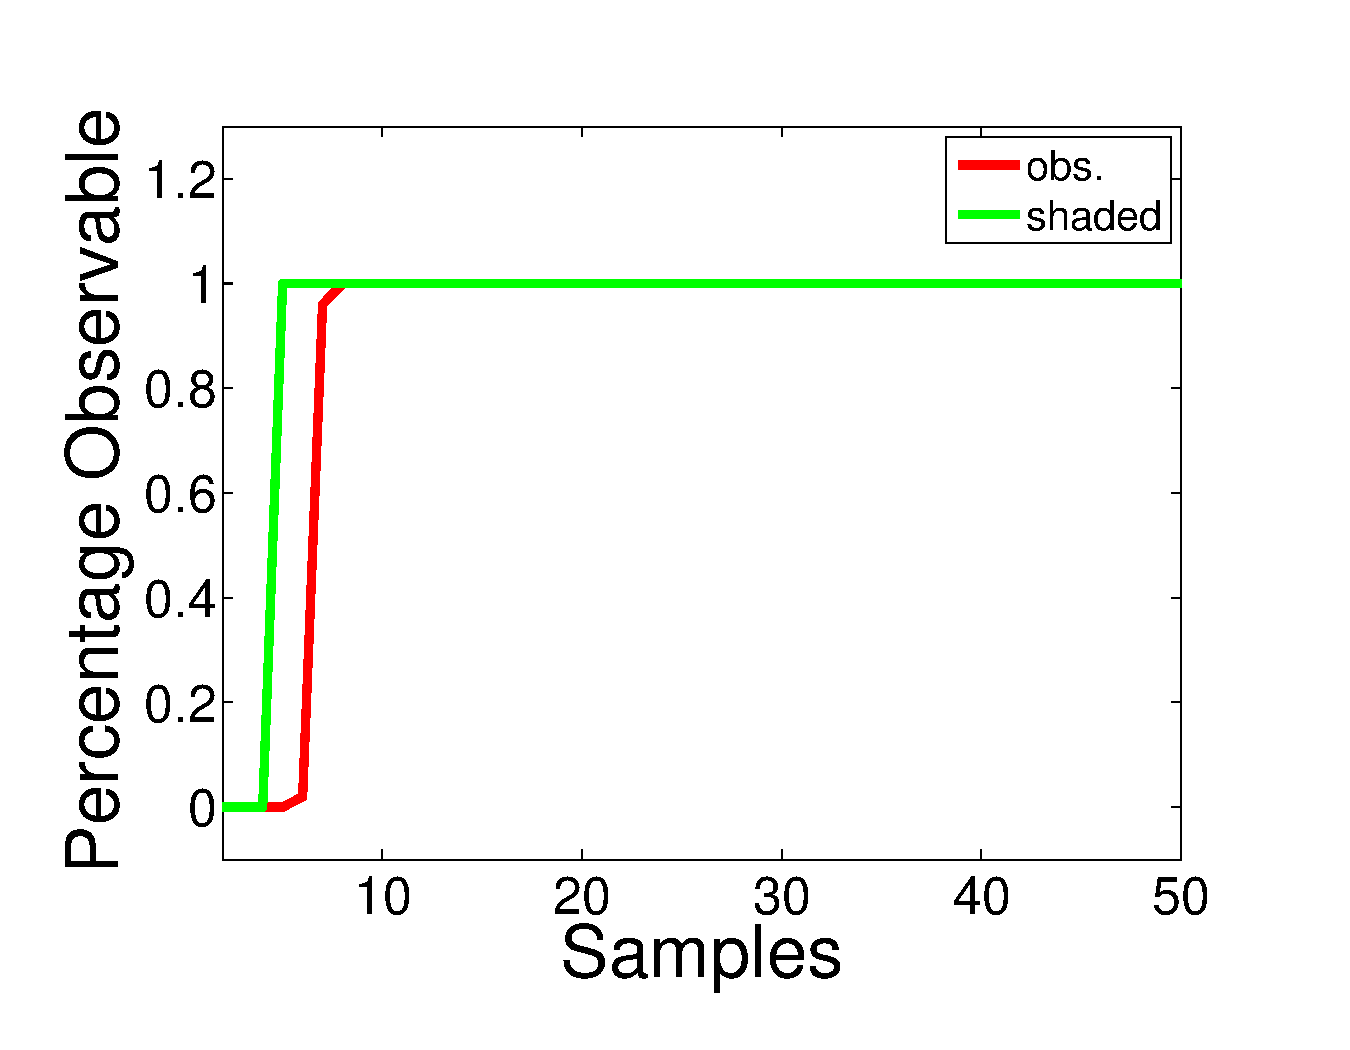
\includegraphics[width=0.45\columnwidth]{kernel_observer_50_cents_smooth4_bandwidth_small.pdf}
    \label{fig:kobs_small}}
     \subfloat[Heuristic vs. random]
     {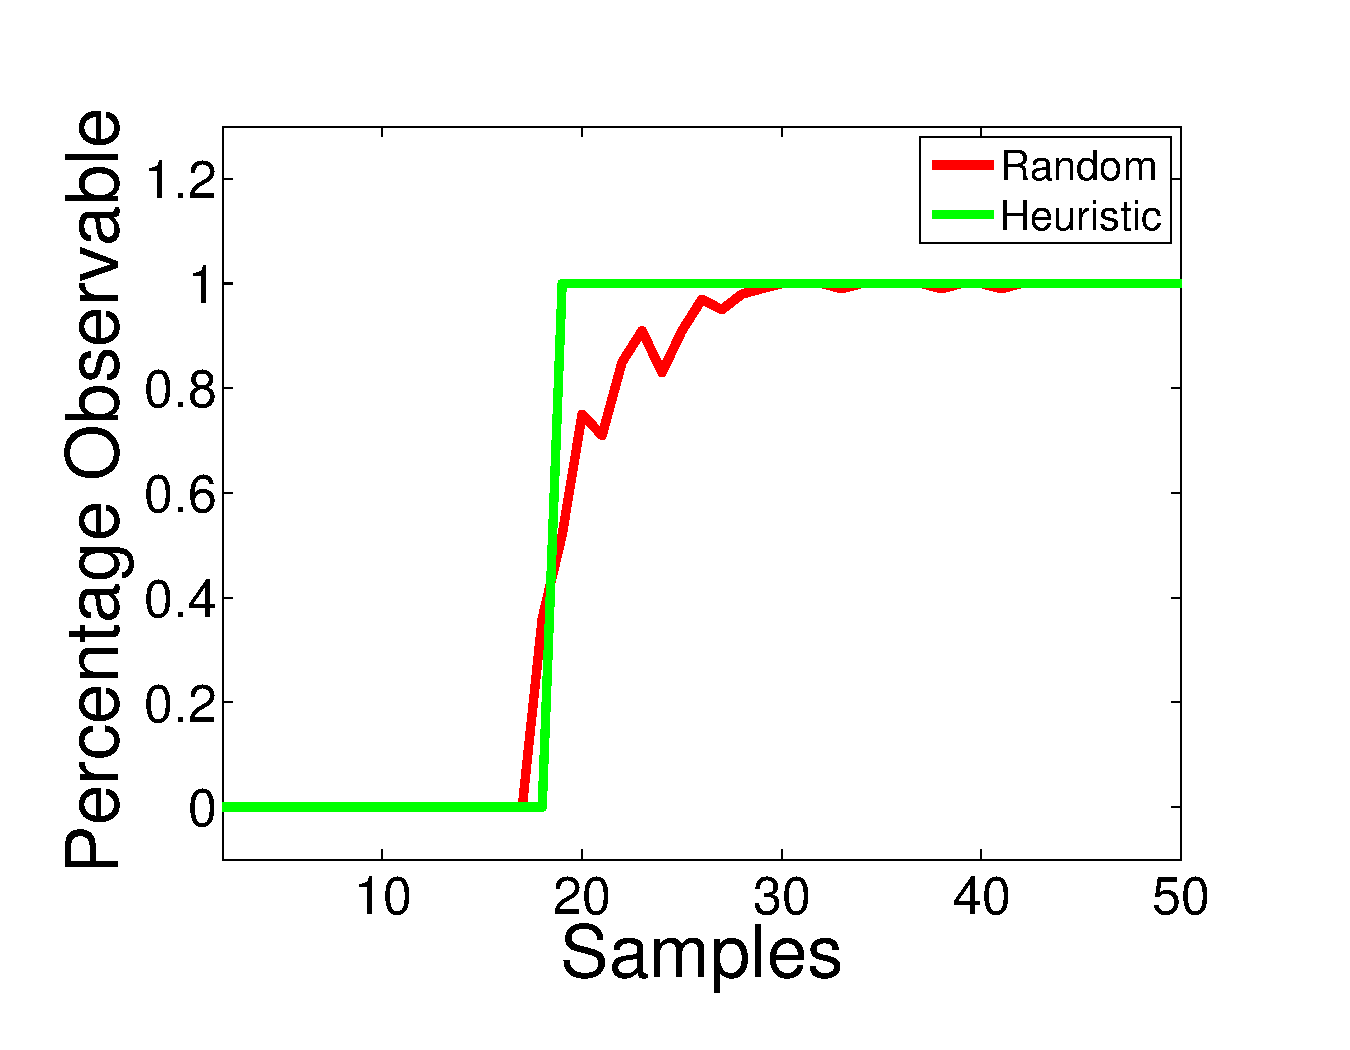
\includegraphics[width=0.45\columnwidth]{rand_average.pdf}
     \label{fig:sample_observability}}  
    \caption{Kernel observability results.}
%\end{figure}
%\begin{figure}[tbh] %{r}{0.5\textwidth}
\end{figure} 

\begin{figure}
\centering
\begin{minipage}{0.48\textwidth}
	% \begin{center}
	\centering
	\subfloat[Error (boxplot)]{
		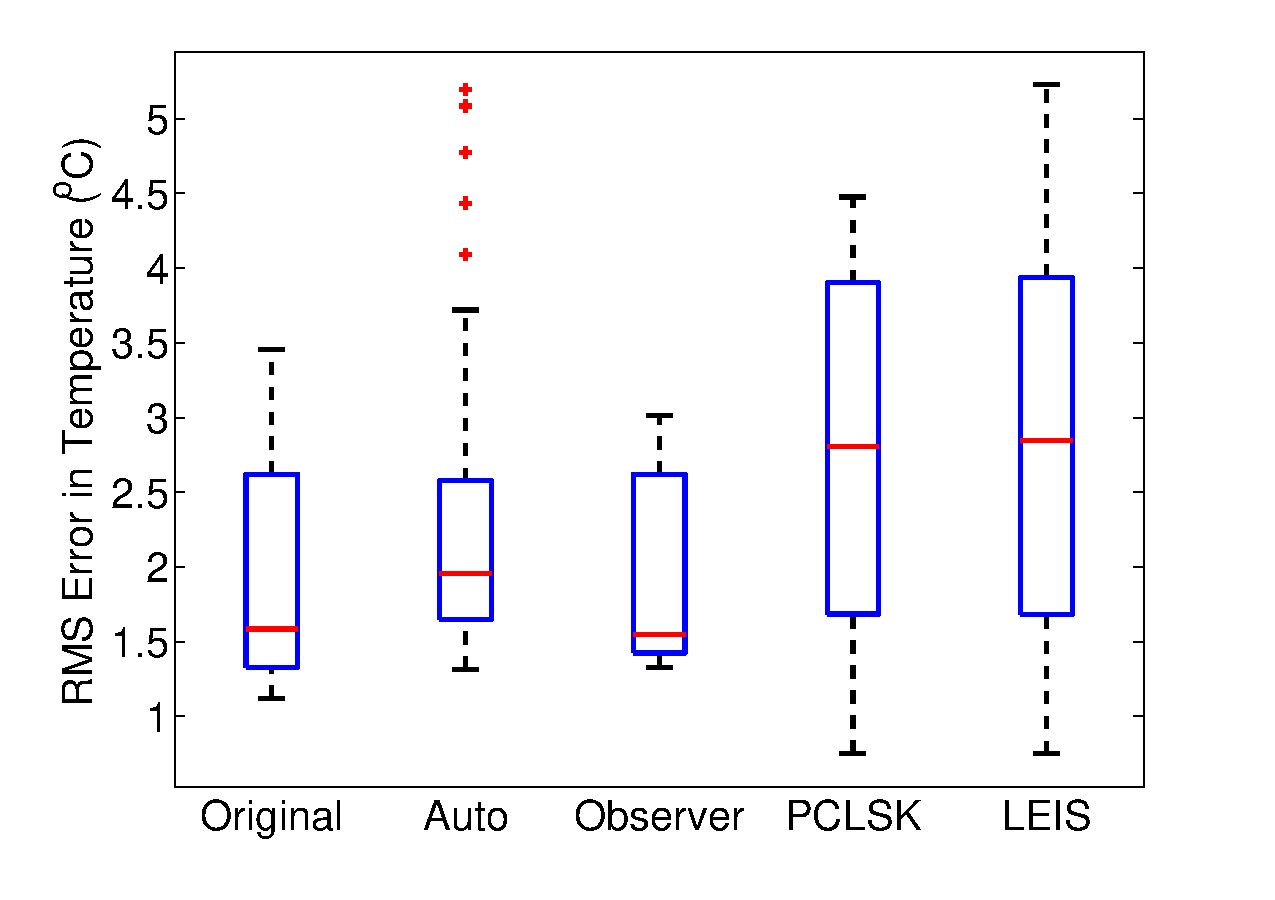
\includegraphics[width=0.45\columnwidth]{box_plot_intel} \label{fig:intel_boxplots} } %pathfinder_errors_boxplot_2012_all_models_night.pdf
	\subfloat[Error (time-series)]
	{
		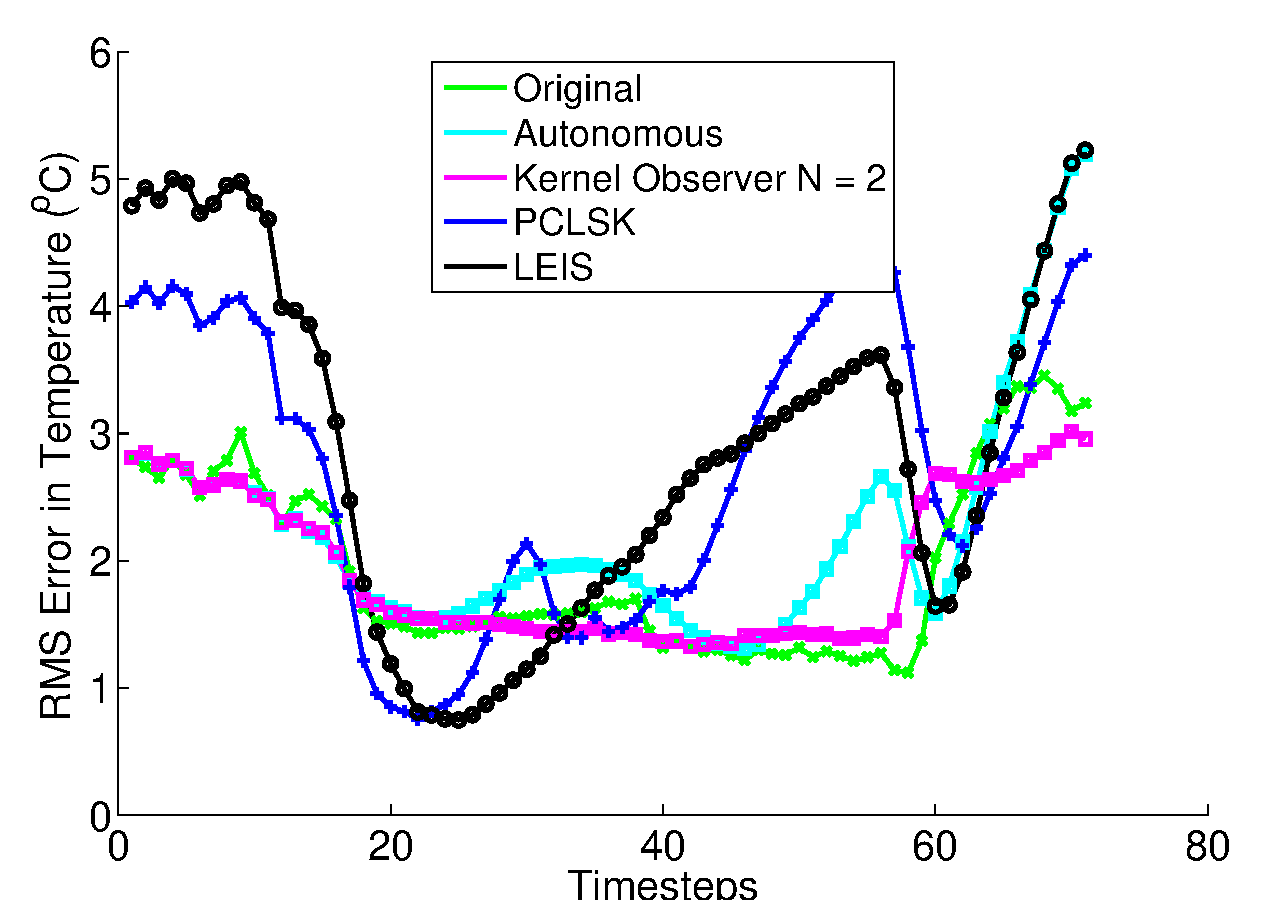
\includegraphics[width=0.45\columnwidth]{Intel_comp} \label{fig:intel_comp}}
	\caption{Comparison of kernel observer to PCLSK and LEIS methods on Intel Berkeley dataset.}     \label{intel}
\end{minipage}
\begin{minipage}{0.48\textwidth}
	
		\subfloat[Error (boxplot)]{
		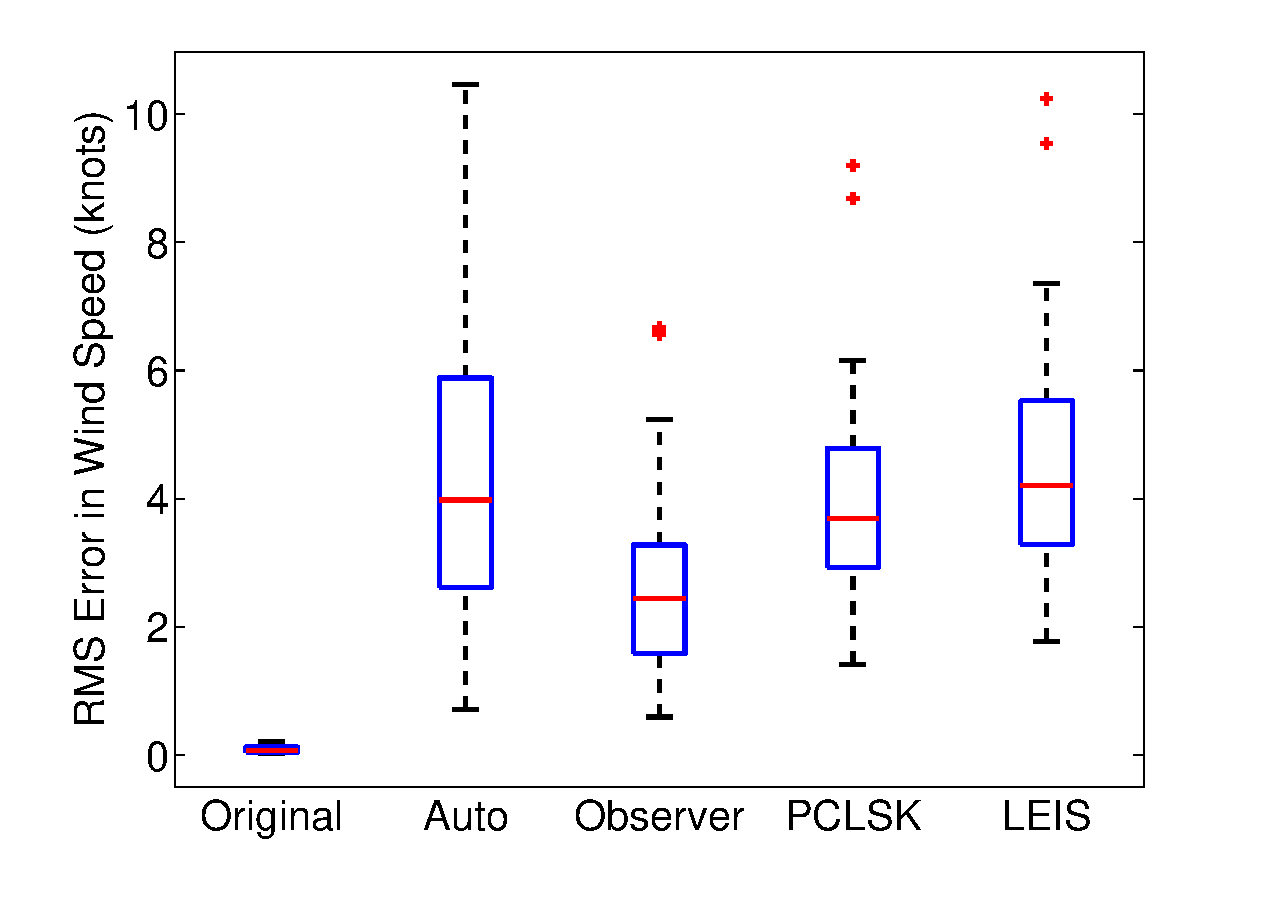
\includegraphics[width=0.45\columnwidth]{box_plot_irish} \label{fig:irish_boxplots} }
		\subfloat[Error (time-series)]{
			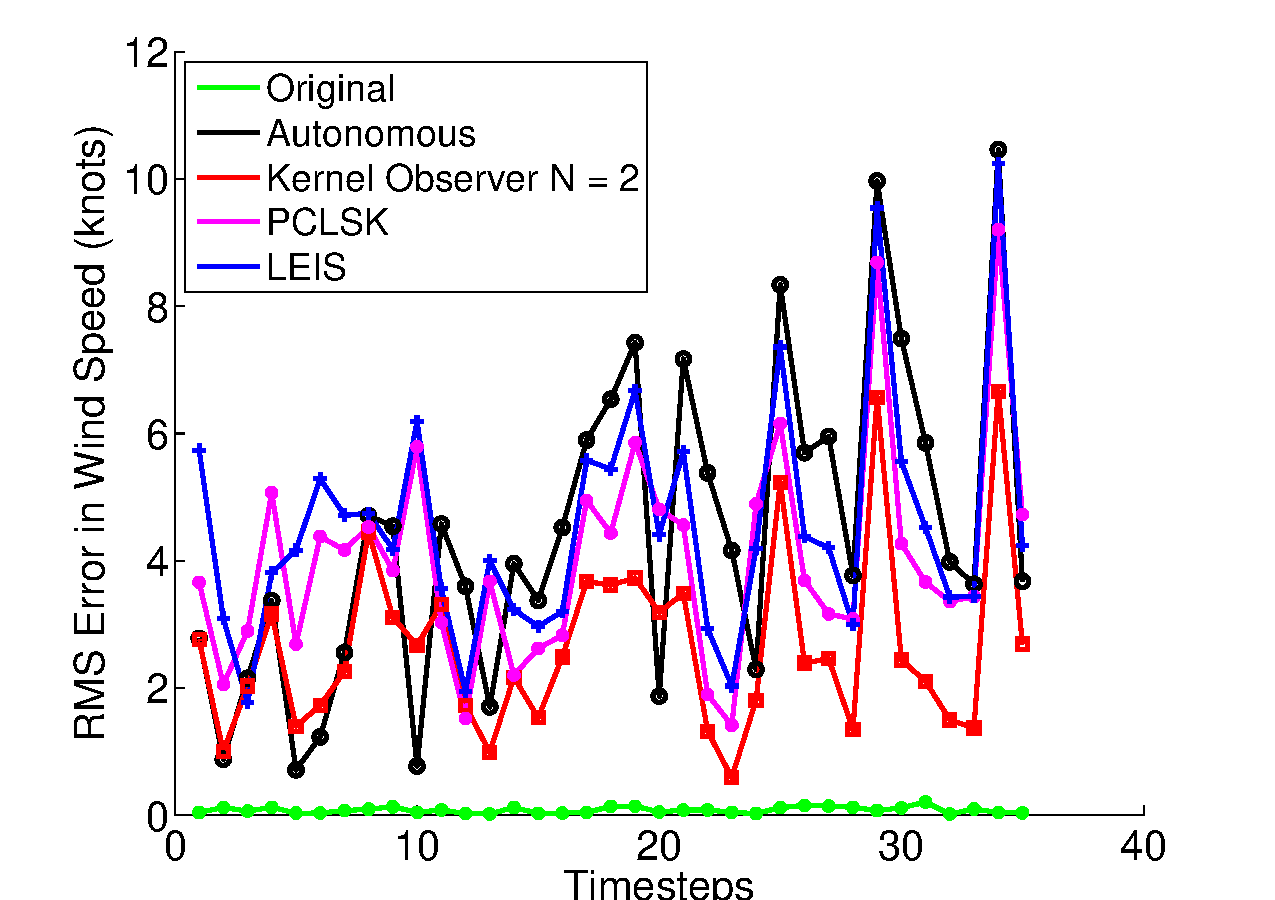
\includegraphics[width=0.45\columnwidth]{irish_wind_comp} \label{fig:irish_comp} }
		\caption{Comparison of kernel observer to PCLSK and LEIS methods on Irish Wind dataset.}\label{irish}
\end{minipage}
\begin{minipage}{0.48\textwidth}
	
		\subfloat[Error (boxplot)]{
		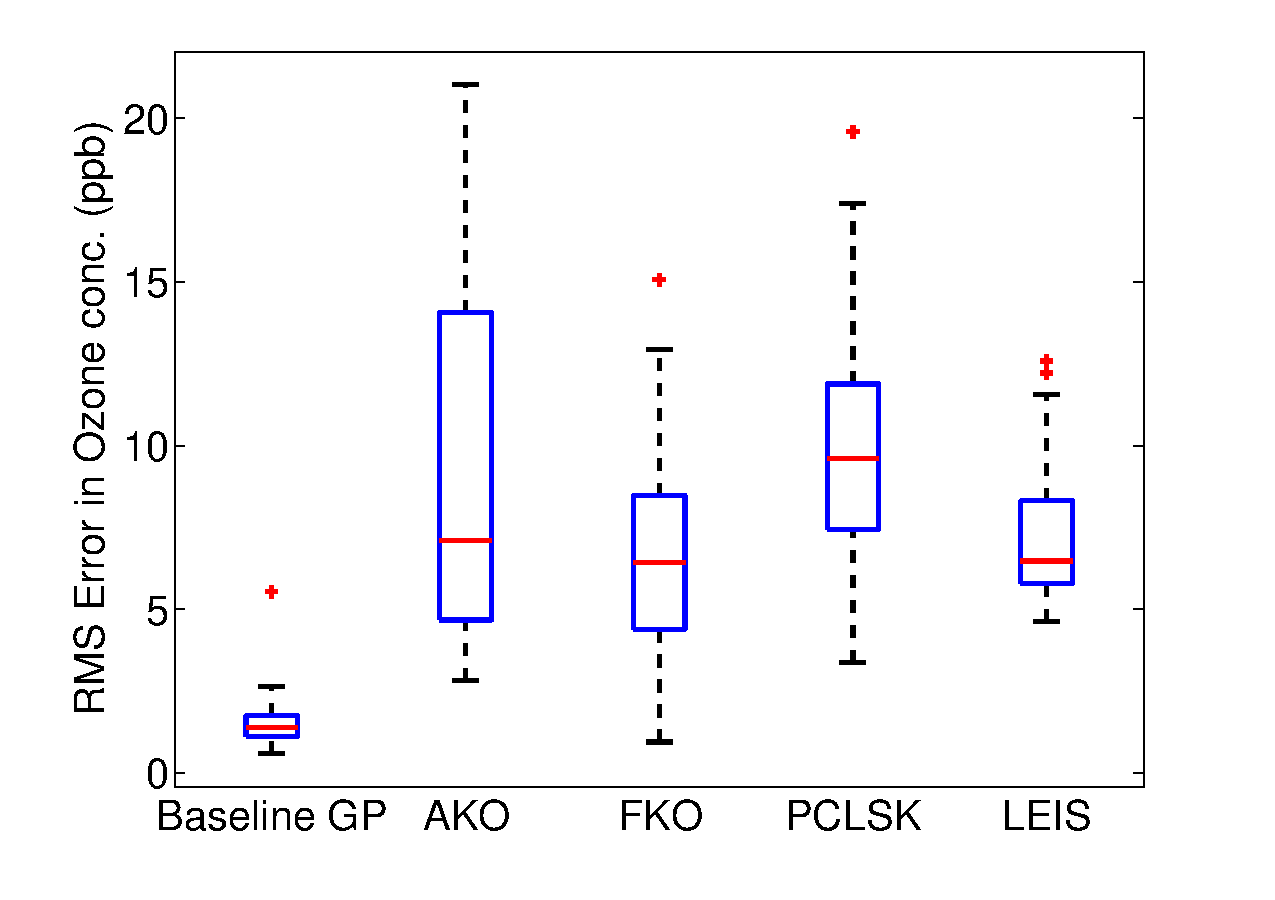
\includegraphics[width=0.45\columnwidth]{box_plot_ozone} \label{fig:ozone_boxplots} }
		\subfloat[Error (time-series)]{
			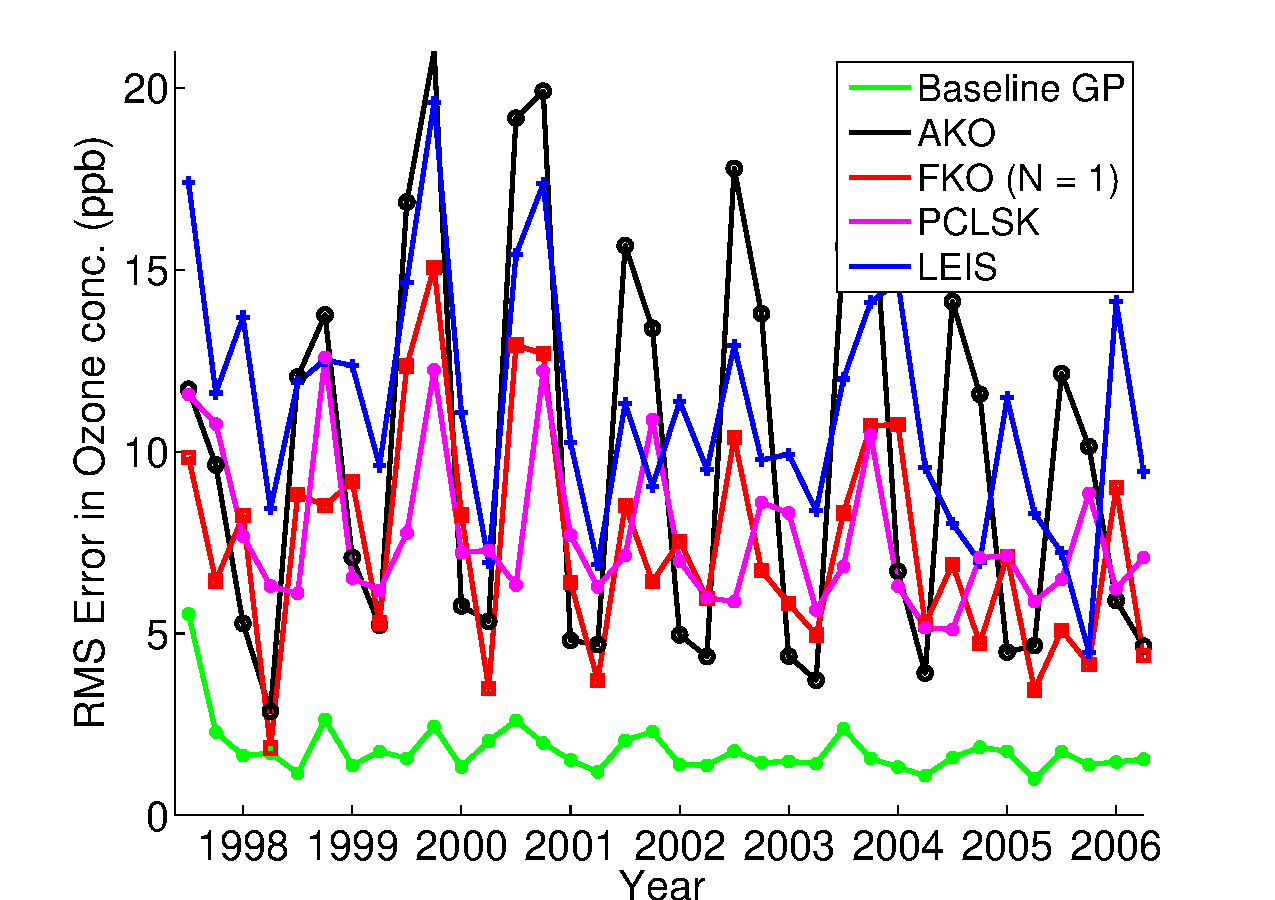
\includegraphics[width=0.45\columnwidth]{ozone_time_series} \label{fig:ozone_comp} }
		\caption{Comparison of kernel observer to PCLSK and LEIS methods on Irish Wind dataset.}\label{ozone}
\end{minipage}
\end{figure}
\begin{figure}
	\centering
	\subfloat[Raw Satellite Data]{
	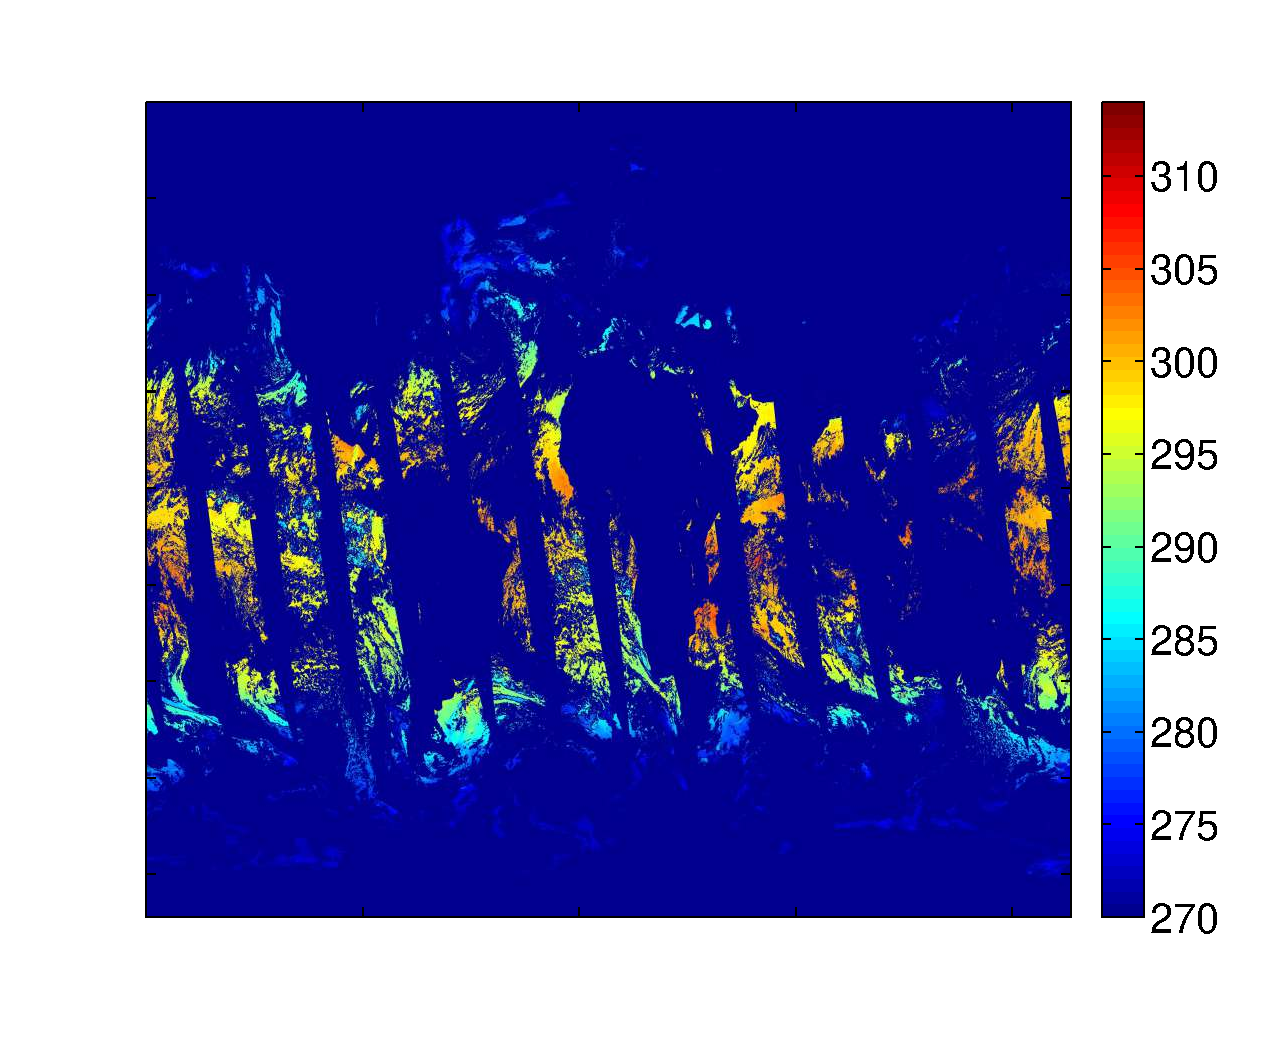
\includegraphics[width=0.4\columnwidth]{pathfinder_raw_data_example}
	\label{fig:Rawpathfinder} }
	\subfloat[AKO estimate]{
	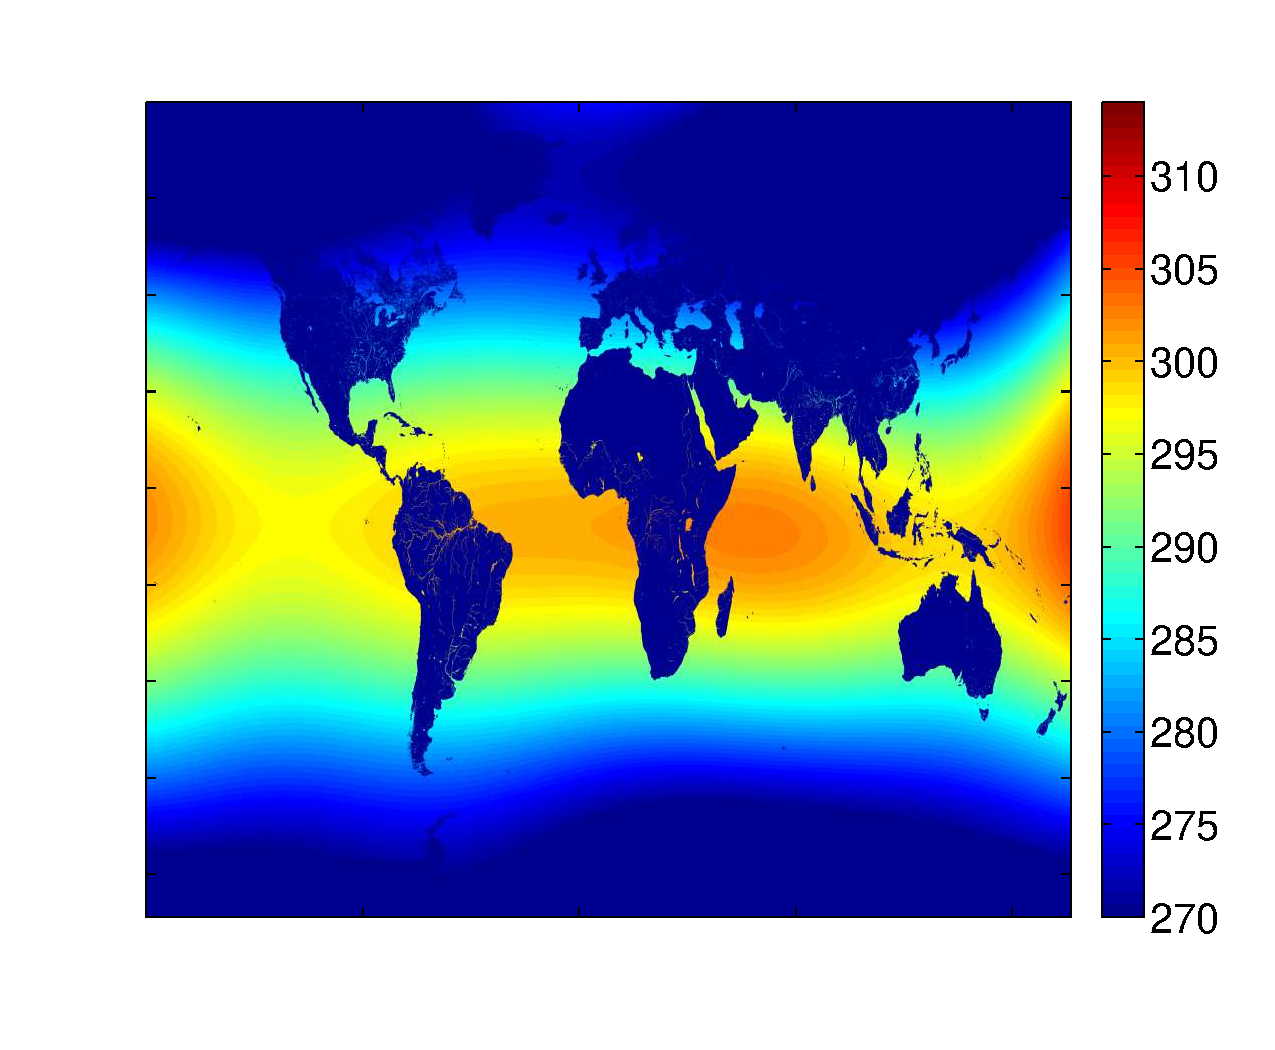
\includegraphics[width=0.4\columnwidth]{pathfinder_inference_example}
	\label{fig:pathfinder} }
	
	\subfloat[Error-day (time-series)]{
		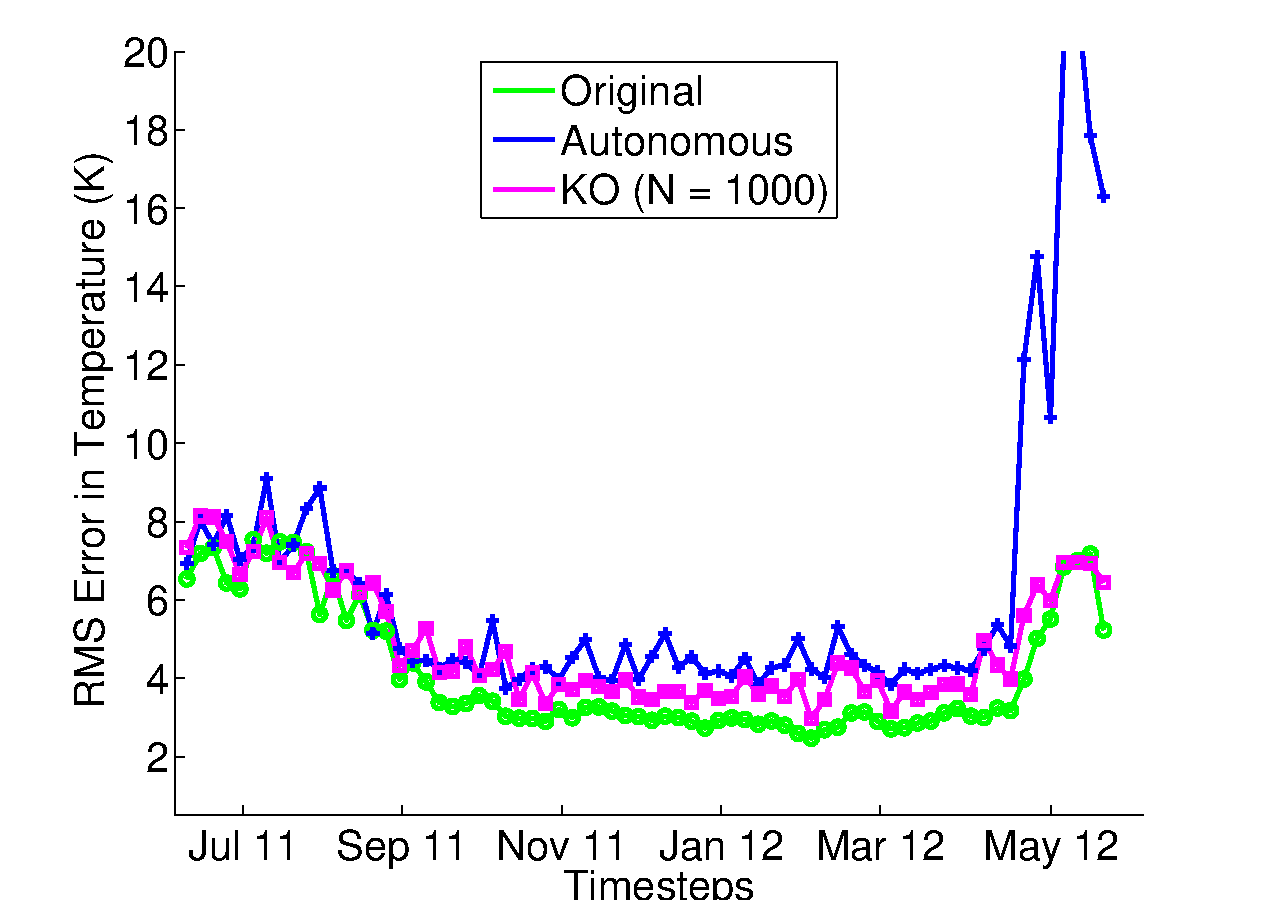
\includegraphics[width=0.4\columnwidth]{time_series_day} \label{fig:time_series_day} }
	\subfloat[Error-night (time-series)]{
		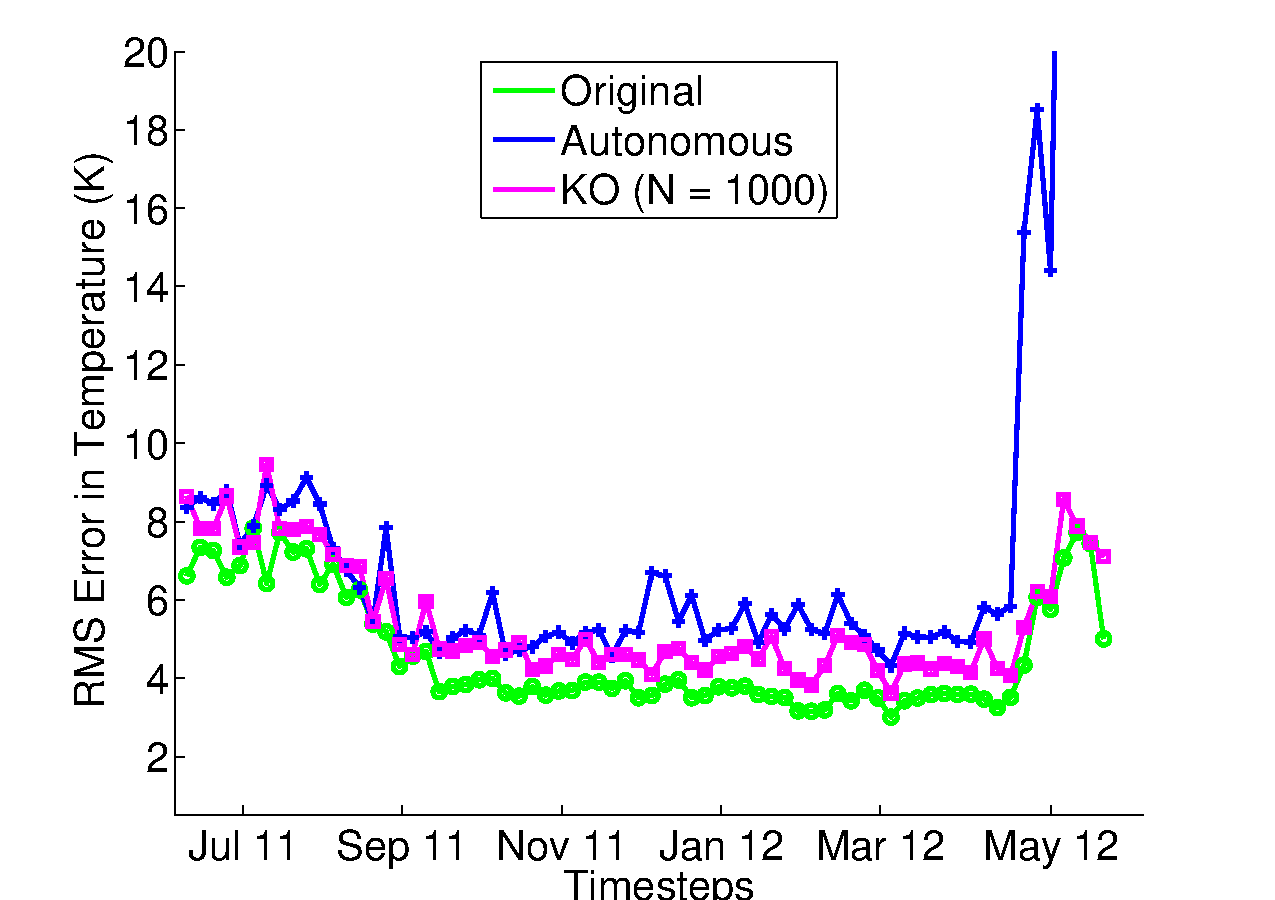
\includegraphics[width=0.4\columnwidth]{time_series_night} \label{fig:time_series_night} }
	 %pathfinder_errors_boxplot_2012_all_models_night.pdf
	 
	\subfloat[Error-day (box-plot)]{
		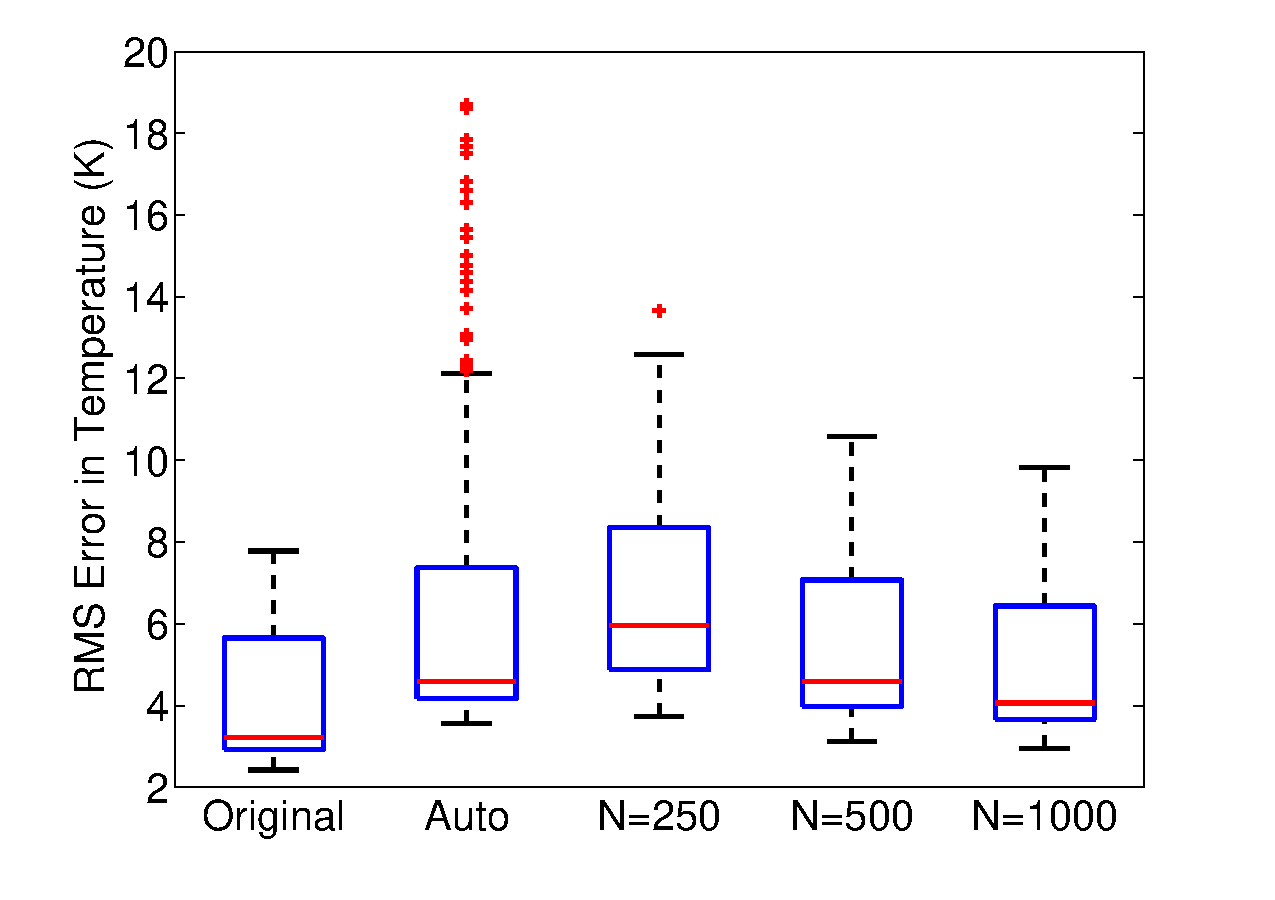
\includegraphics[width=0.4\columnwidth]{box_plot_path_day} \label{fig:pathfinder_errors_boxplots_day} }
	\subfloat[Error-night (box-plot)]{
		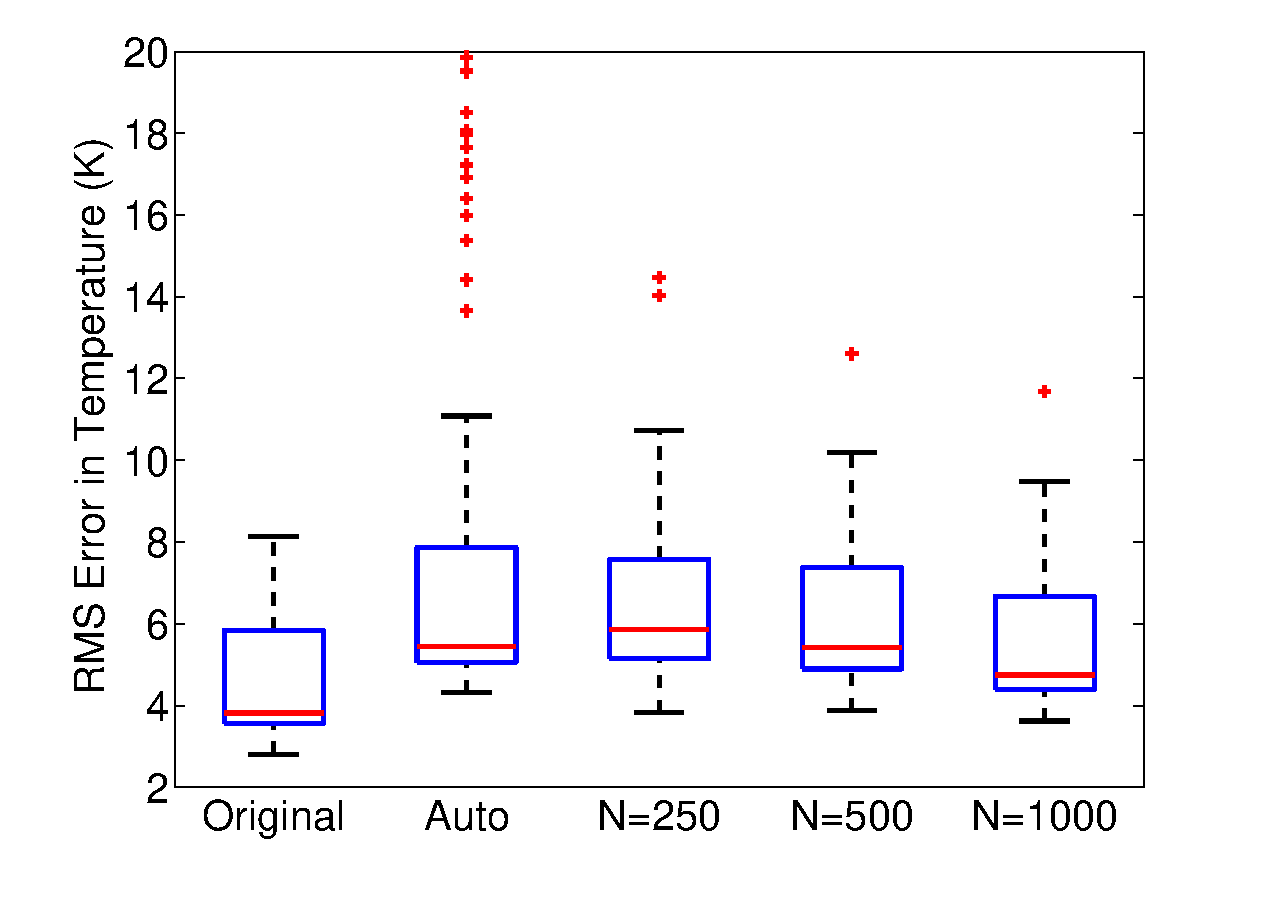
\includegraphics[width=0.4\columnwidth]{box_plot_path} \label{fig:pathfinder_errors_boxplots} }
		
	\subfloat[Estimation time (day)]
	{
		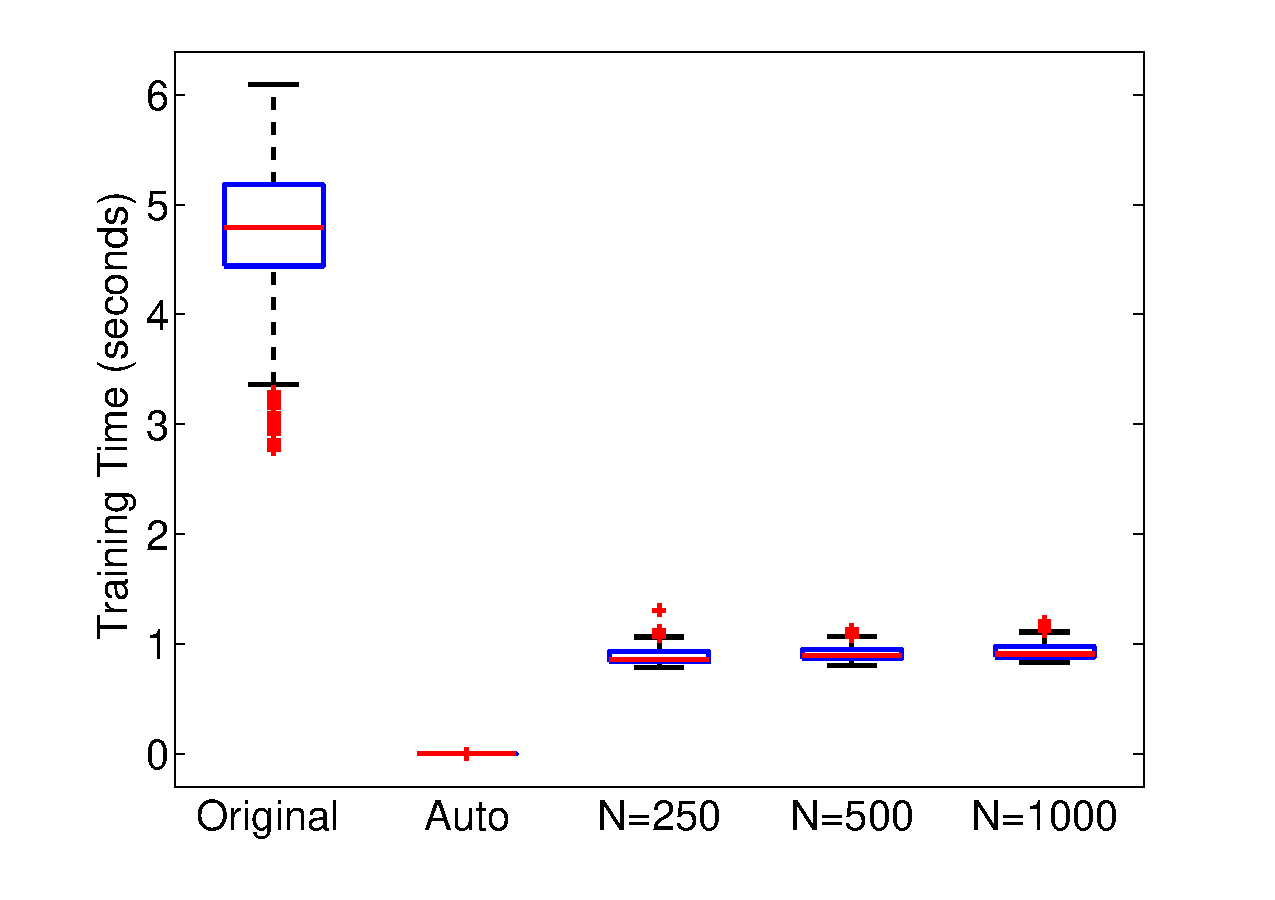
\includegraphics[width=0.4\columnwidth]{box_plot_path_day_time} \label{fig:pathfinder_tr_times_boxplots_day}}
	\subfloat[Estimation time (night)]
	{
		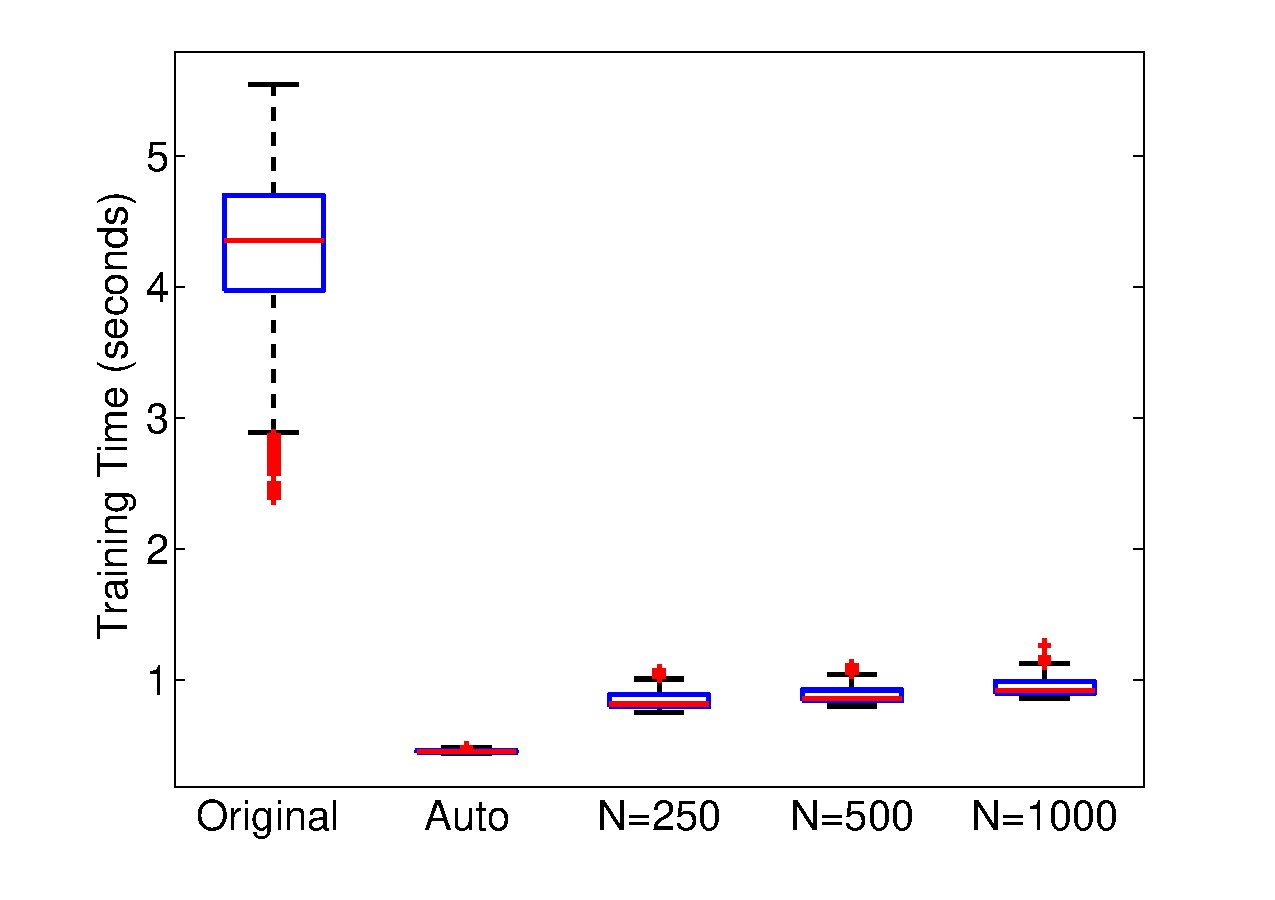
\includegraphics[width=0.4\columnwidth]{box_plot_path_time} \label{fig:pathfinder_tr_times_boxplots_night}}
		
%	\subfloat[Estimation time (night)]
%	{
%		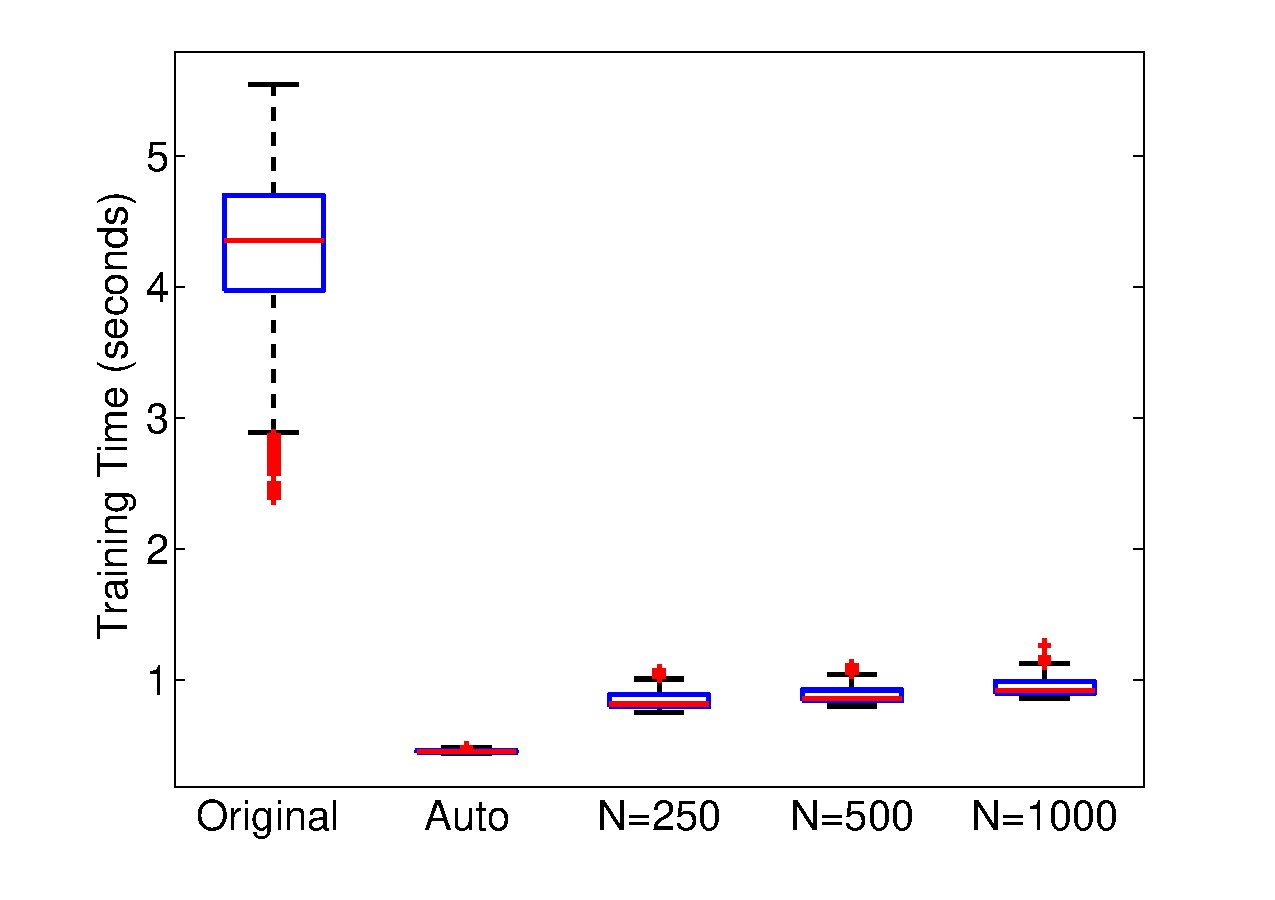
\includegraphics[width=0.33\columnwidth]{box_plot_path_time} \label{fig:pathfinder_tr_times_boxplots}}
	%pathfinder_errors_boxplot_2012_all_models_night.pdf
	%pathfinder_tr_times_boxplot_2012_all_models_night   
	\caption{Performance of the kernel observer over AVVHR satellite 2012 data with different numbers of observation locations.}
\end{figure}

\begin{figure*}
    \centering
    \hspace{-0.3in}\subfloat[6th May]{
	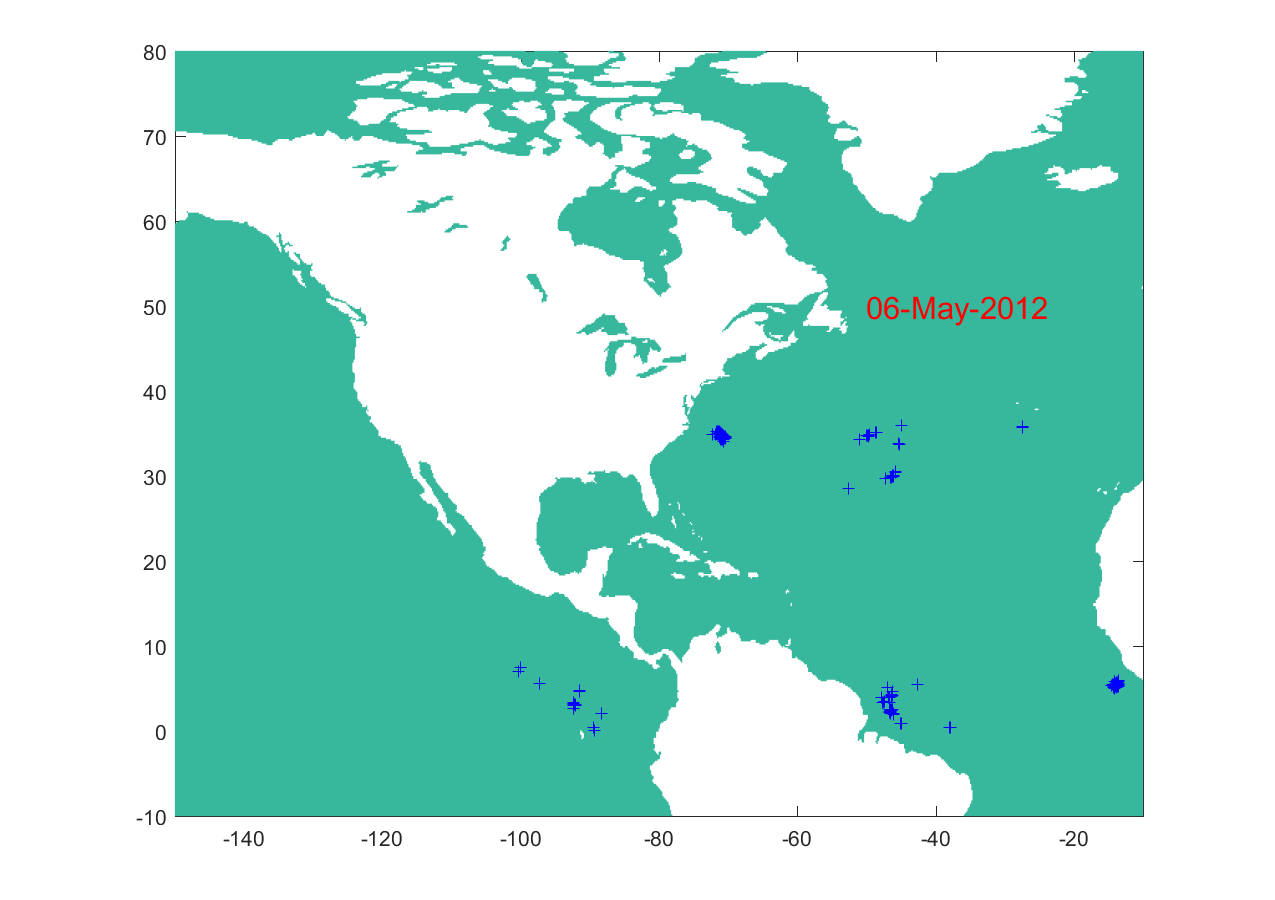
\includegraphics[scale=0.22]{May6}
	\label{fig:May6 } }
	\hspace{-0.5in}
	\subfloat[7th May]{
	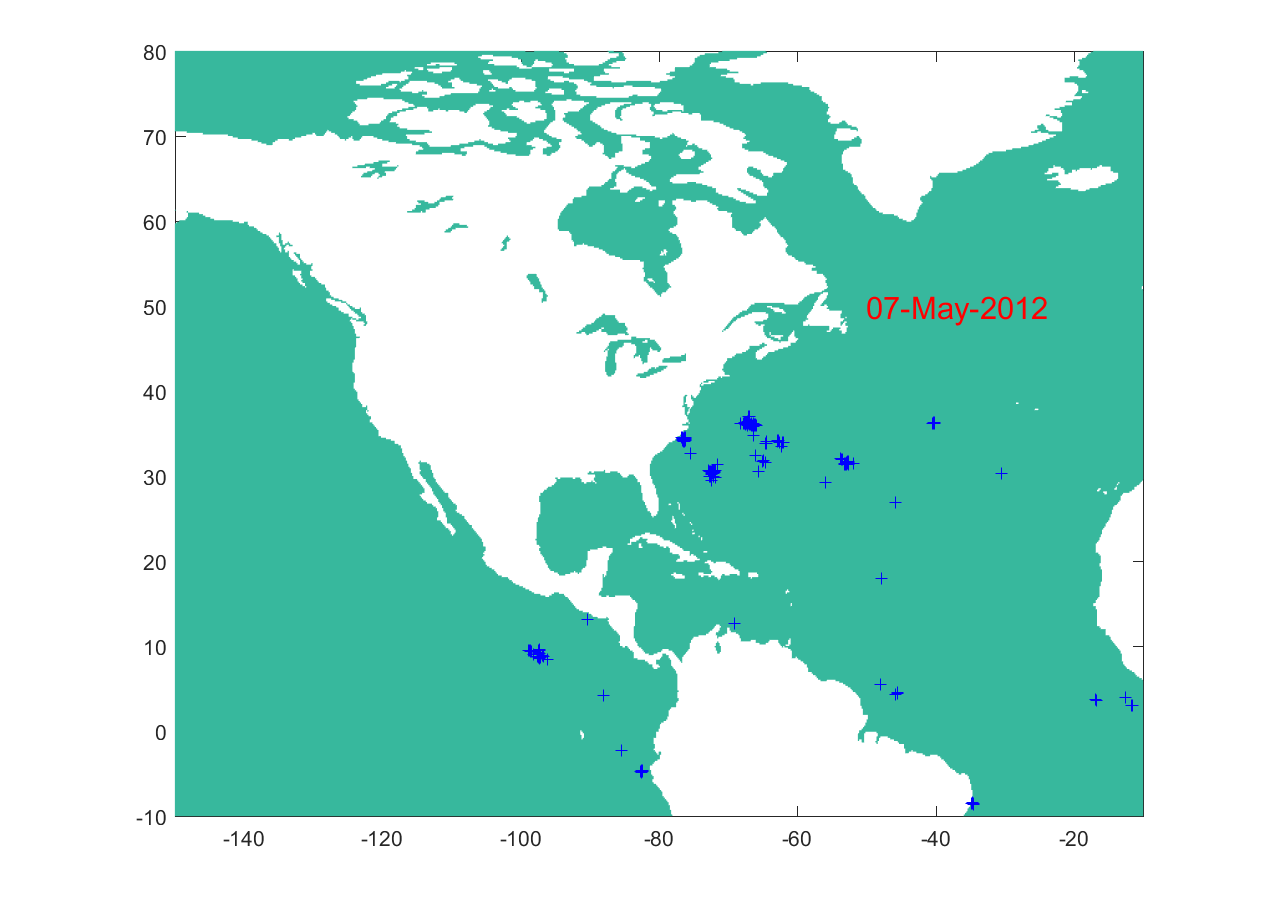
\includegraphics[scale=0.22]{May7}
	\label{fig:May7 } }
	\hspace{-0.5in}
	\subfloat[28th May]{
	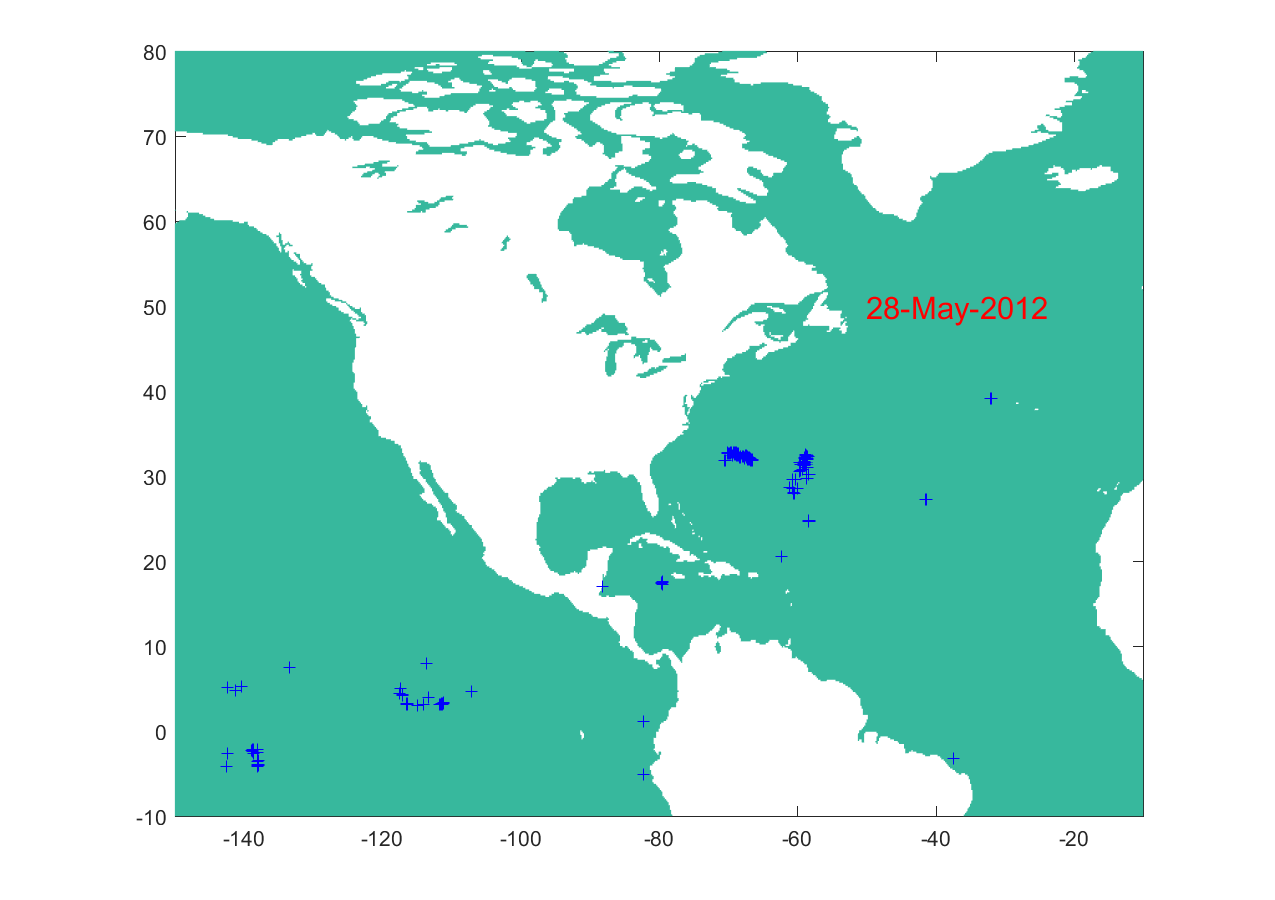
\includegraphics[scale=0.22]{May28}
	\label{fig:May28 } }
	\hspace{-0.5in}\subfloat[29th May]{
	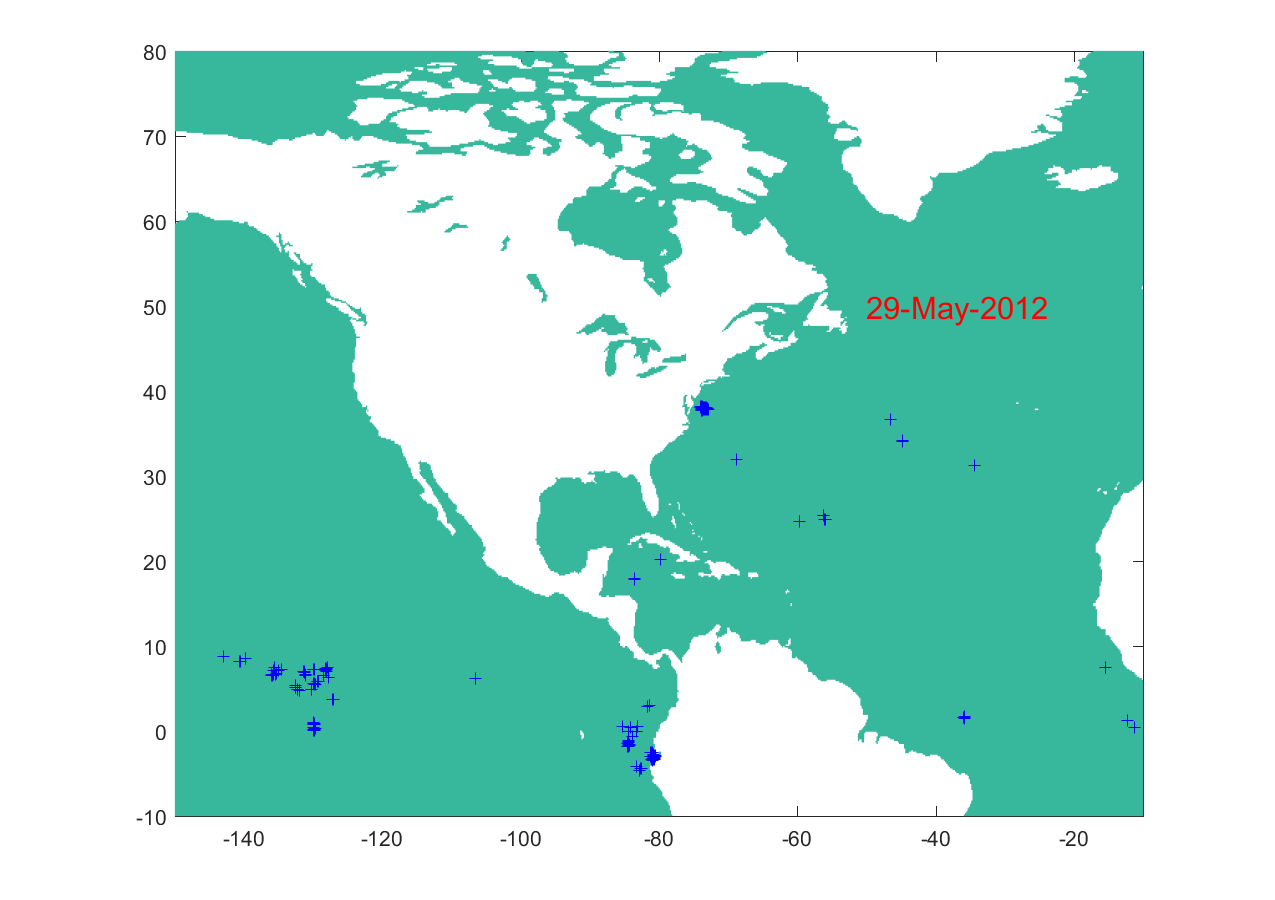
\includegraphics[scale=0.22]{May29}
	\label{fig:May29 } }
	\caption{Locations of weather anomaly obtained based on the error between the acutual temperature and the prediction of autonomous kernel observer. Landmass is shown in white and the ocean is in green. Locations marked have error greater than two standard deviations above the mean error. }
	\label{fig:anomaly}
\end{figure*}



\subsection{Predicting evolution of weed density in agricultural fields}\label{sec:weed}

As a proof-of-concept in applying our methods for learning dynamics and/or inferring the state of spatiotemporally-evolving systems to real, relevant problems, we present our work with weed growth in agricultural fields.

Past work has presented detailed analysis of weed growth models, in which measurements of seed bank density for various species of weeds were conducted \cite{Nordby2018, schutte2014common, sellers2003comparative, horak2000growth}. In order to generate data upon which to test our methods, we implemented a weed growth simulation model whose rate of seedling emergence agrees with that found in the above research. A Poisson process is utilized to simulate the temporal evolution of emergence events. This assumption is reasonable over the short time scales in which robots may fully weed a field.
\vskip 1em
Other work in the field of crop science \cite{mulugeta1997seed, mulugeta1999seasonal} has shown that the spatial variation in the seed bank density for some species of weeds may be modeled via the Gini Coefficient of Concentration (GCC). This model is accurate for common waterhemp (\textit{Amaranthus tuberculatus}), and thus we found it useful in our simulation of the spatial distribution of the seed bank density. For more reading. see \cite{davis2013seed, werle2014predicting} regarding the relationship between seed bank emergence patterns and environmental conditions such as temperature and moisture.

The weed growth simulation is based on Bernoulli random variables, operating on a matrix of cells, each $0.8$ m$^2$, comprising a gridded field of $0.4$ hectares, or a cellular automata model \cite{chopard1998cellular}. Seeds emerge from a limited seed bank, forming a binomial distribution over time. The parameters used, summarized in Table \ref{tab:weedparams}, are aligned with the growth model for common waterhemp determined in \cite{mulugeta1997seed}. The initial density of the seed bank in each cell is $S_0$ on average (between $600$ and $1560$ seeds per cell). However, at the start of the simulation, the seed bank density in each cell, $S_0(x, y)$, is chosen so that Gini Coefficient of Concentration (GCC) between all the cells, used to ensure the relative density of weeds aligns with that seen in real experiments, is from $0.31$ to $0.35$, as was determined experimentally in \cite{mulugeta1997seed}. The field is first divided into fifty patches of weeds, with centers chosen uniformly at random, and sizes from zero to twenty cells in each dimension. Each cell has an initial density between zero and twenty percent of $S_0$, chosen uniformly at random. Finally, for each patch of weeds, up to an additional $S_0$ weeds are added to each cell within each patch, so that the density of each patch follows a normal distribution. 

\begin{table}[h]
	\centering
	\caption{Seed Bank Density Parameters} \label{tab:weedparams} 
	\begin{center}
		\begin{tabular}{ | l | l | l | l | l |}
			\hline
			\textbf{Parameter} & GCC         & $S_0$ (seeds/cell)       & Num. of Patches & Patch Size (Cells in X and Y)  \\ \hline
			\textbf{Range}     & [0.31,0.35] & [600,1560] & 50  & [0,20]  \\ \hline
		\end{tabular}
	\end{center}
\end{table}


Upon initialization of the simulation, a certain number of days, $d_0$, are allowed to elapse before weeding starts. The number of emerging weeds in each cell, $N_{{\text{emerge}}}$, is a randomly generated Poisson variable with mean, $\lambda \left( {x,y,t} \right) $, such that $90$ percent of the seed bank, $S\left( {x,y,t} \right)$, emerges in $T_\text{total}$, which is two months. This emergence rate is aligned with past work \cite{Nordby2018,schutte2014common, werle2014predicting, sellers2003comparative, horak2000growth},  which all present measurements of the seed bank densities for various species of weeds, and provide an analysis of weed growth models for these species.

The weed density in each cell, $\zeta \left( {x,y,t} \right) $, grows as seeds emerge from the seed bank. The maximum weed height at each cell, $\delta \left( {x,y,t} \right)$, increases from zero height at a fixed rate $\Gamma$ inches per day.

Of course, robots going out to weed a field only have access to sparse data about weed density and height, and no data about the seedbank or about the field in locations that have not been visited. For this reason, we have trained a Kernel observers model on the weed density data generated by our simulations, so that robots in the field can quickly infer the state of the field globally from sparse measurements.

We used a Radial Basis Function (RBF) kernels with a bandwidth approximately 5 cells (4.5 meters) wide. These were centered throughout the domain using Csato \& Opper's algorithm. After training a GP on each snapshot of the data, we obtained a weight vector trajectory. We used linear least squares do determine the best linear transition in the weight space for this trajectory. Below we have included images of system as predicted by feeding forward the initial condition through this linear transition, as a comparison with the original data. The model is able to approximate the weed density growth data very well, with percent error averaging 5\%.

\begin{figure*}[h] %{r}{0.5\textwidth}
	\centering
	\subfloat[Snapshot 2]{
		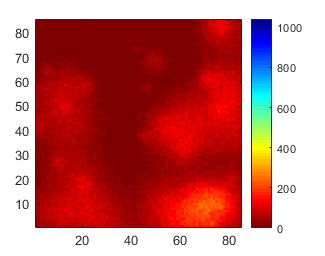
\includegraphics[width=0.23\textwidth]{weed2}		}
	\subfloat[Snapshot 28]{
		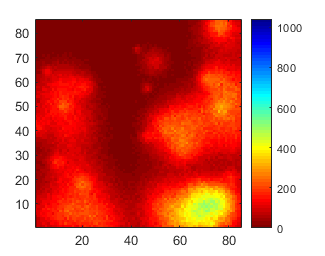
\includegraphics[width=0.23\textwidth]{weed28}		}
	\subfloat[Snapshot 54]{
		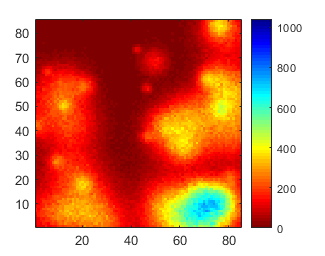
\includegraphics[width=0.23\textwidth]{weed54}		}
	\subfloat[Snapshot 80]{
		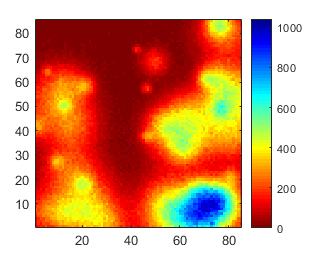
\includegraphics[width=0.23\textwidth]{weed80}		}\\
	\subfloat[Snapshot 2]{
		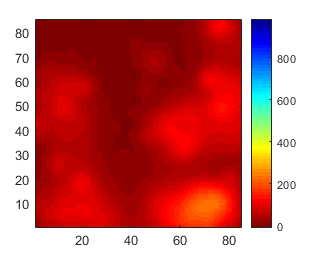
\includegraphics[width=0.23\textwidth]{weed2_egp}		}
	\subfloat[Snapshot 28]{
		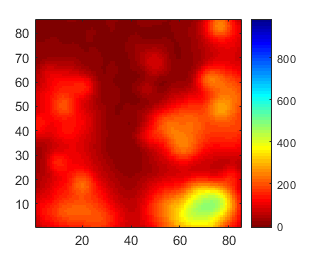
\includegraphics[width=0.23\textwidth]{weed28_egp}		}
	\subfloat[Snapshot 54]{
		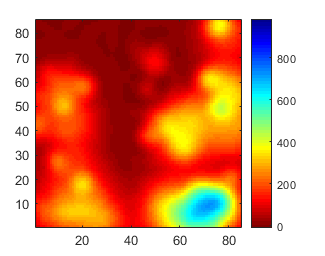
\includegraphics[width=0.23\textwidth]{weed54_egp}		}
	\subfloat[Snapshot 80]{
		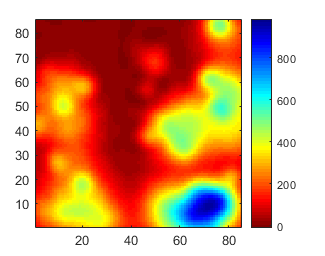
\includegraphics[width=0.23\textwidth]{weed80_egp}		}
	
	\caption{Visualization of Weed Density Growth over 20 days, original (a-d), E-GP (e-h)}
	\label{fig:weed_egp}
\end{figure*}



\subsection{Control of a linear PDE} %with AVHRR Satellite data}
We then employed kernel controllers for controlling an approximation to the scalar diffusion equation $u_t = bu_{xx}$ on the domain $\dom=[0,1]$, with $b=0.25$. The solution to this equation is infinite-dimensional, so we chose a kernel $\kernel(x,y) = e^{-(\|x-y\|^2/2\s^2)}$, and a set of atoms  $\Atoms=\shCentLong$, $c_i\in\dom$, with $\ncent = 25$ generating $\fspaceC$, the space approximating $\fspace$, and another set of atoms $\AtomsControl=\{\fmap(d_1),\dots,\fmap(d_{\ncontrol})\}$, $d_j\in\dom$,
$\ncontrol=13$, generating the control space $\fspaceD$. The number of, and the location of the observations was chosen to be the same as that of the actuation locations $d_j$. First, tests (not reported here) were conducted to ensure that the solution to the diffusion equation is well approximated in $\fspaceC$. Matrix least-squares was used to infer $\estsysop$. Figure \ref{fig:uncontrolled_pde} shows an example of an initial function $f_{\text{init}}$ evolving according to the PDE.  A reference function $f_{\text{ref}}\in\fspaceC$ was chosen to drive $f_{\text{init}}$ to $f_{\text{ref}}$ under the action of the PDE. Finally, Algorithm \ref{alg:egp_control} was used to control the PDE, driving $f_{\text{init}}$ to $f_{\text{ref}}$; Figure \ref{fig:controlled_pde_error} shows the absolute value of the error between $f_k $ and $f_{\text{ref}}$ as a function of time. 

% We performed experiments to evaluate the number of randomly placed Actuators and Sensors required as compared to the lower bound obtained in Proposition \ref{prop:2}. Results in Table \ref{compare} shows that randomly placing the sensors and actuators works efficiently for lower set of atoms $ \ncent$ in $ \Atoms$.
% 
% \begin{table}
% 	\caption{Number of randomly placed Actuators and Sensors (average $\pm$ variance) required as compared to the lower bound $\minmeas$ obtained in Proposition \ref{prop:2}. }
% 	\label{compare}
% 	\begin{center}
% 		\begin{tabular}{|c||c||c||c|}
% 			\hline
% 			Set of & Lower  & Number of   & Number of  \\
% 			Atoms & bound ($\minmeas$) & Actuators  &  Sensors \\
% 			
% 			\hline
% 			M = 25 & 10 & 10.27 $\pm$ 0.45 & 10.36 $\pm$ 0.50 \\
% 			M = 30 & 13  & 15.26 $\pm$ 0.51 & 15.24 $\pm$ 0.49 \\
% 			M = 35 & 19  & 21.43 $\pm$ 0.54 & 21.35 $\pm$ 0.50 \\
% 			M = 40 & 24 & 33.08 $\pm$ 6.05 & 32.40 $\pm$ 6.0 \\
% 			% M = 30 & 8.5 $\pm$ 0.8 & 8.5 $\pm$ 0.9 & 10.8 $\pm$ 1.4 \\
% 			\hline
% 		\end{tabular}
% 	\end{center}
% \end{table}

\begin{figure}[tbh] %{r}{0.5\textwidth}
    \centering
    \subfloat[Evolution of initial function $f_{\text{init}}$ according to diffusion equation.]{
    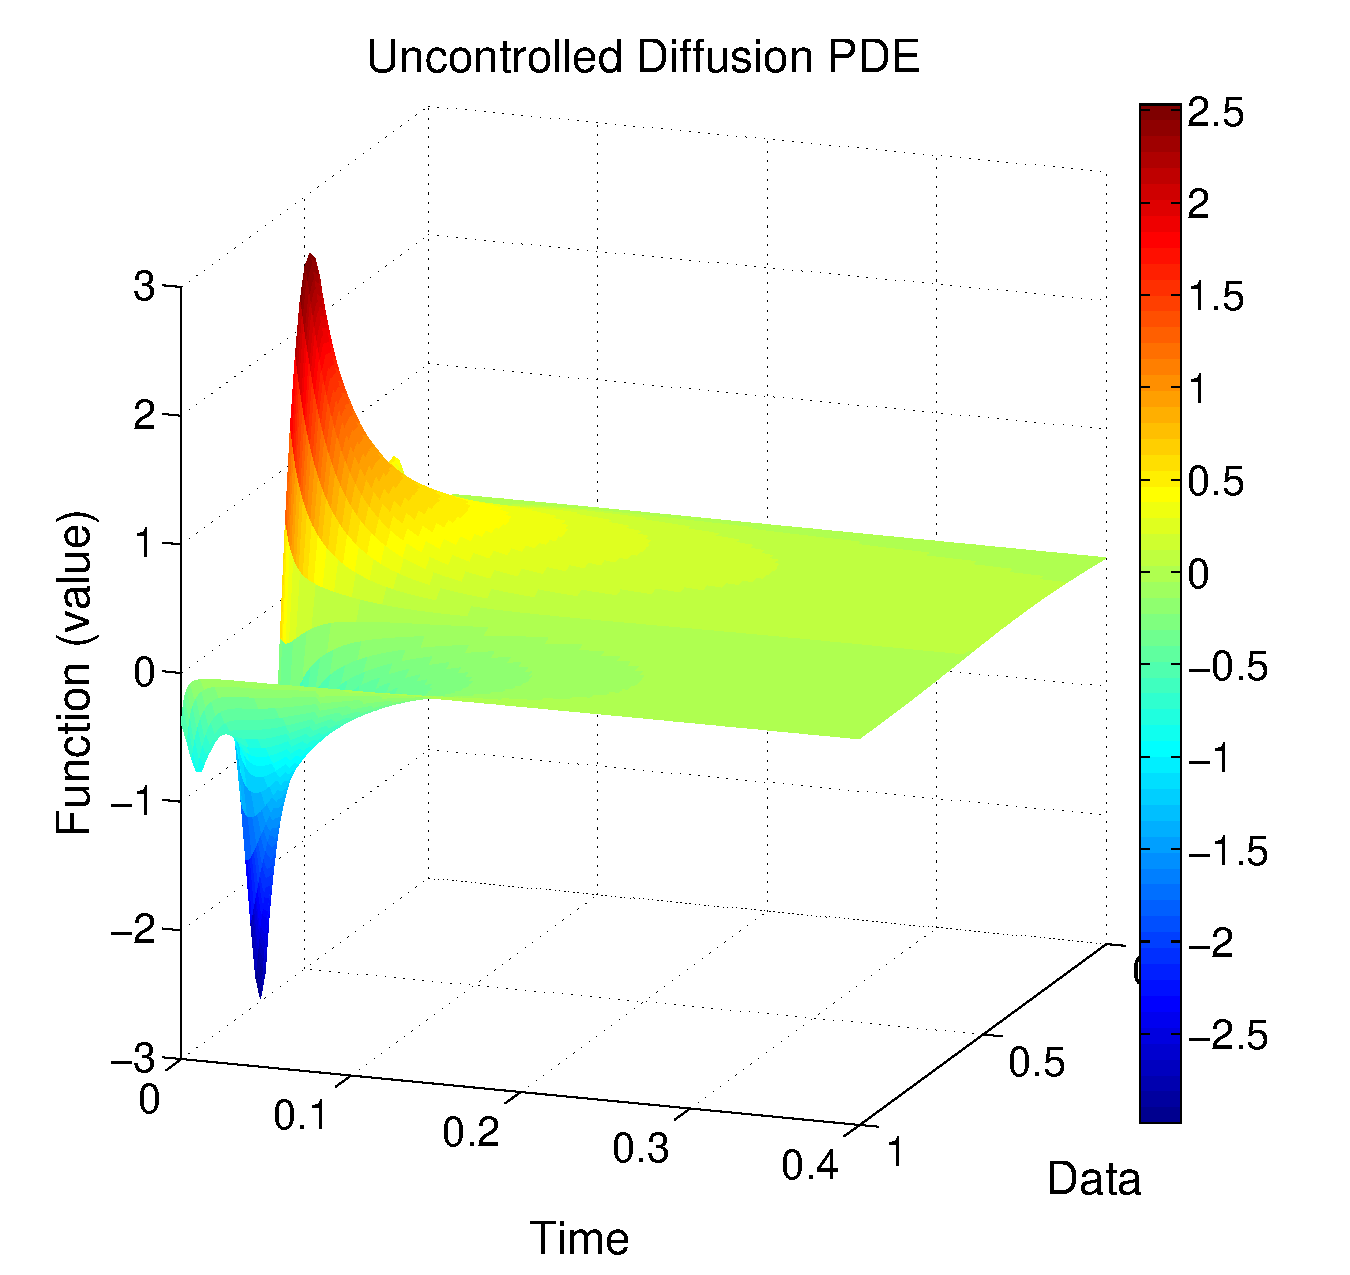
\includegraphics[width=0.45\columnwidth]{uncontrolled_pde_heat.pdf} 
    \label{fig:uncontrolled_pde}}
%     \subfloat[Initial function $f_{\text{init}}$ driven to $f_{\text{ref}}$ using kernel controller.]
%     {
%     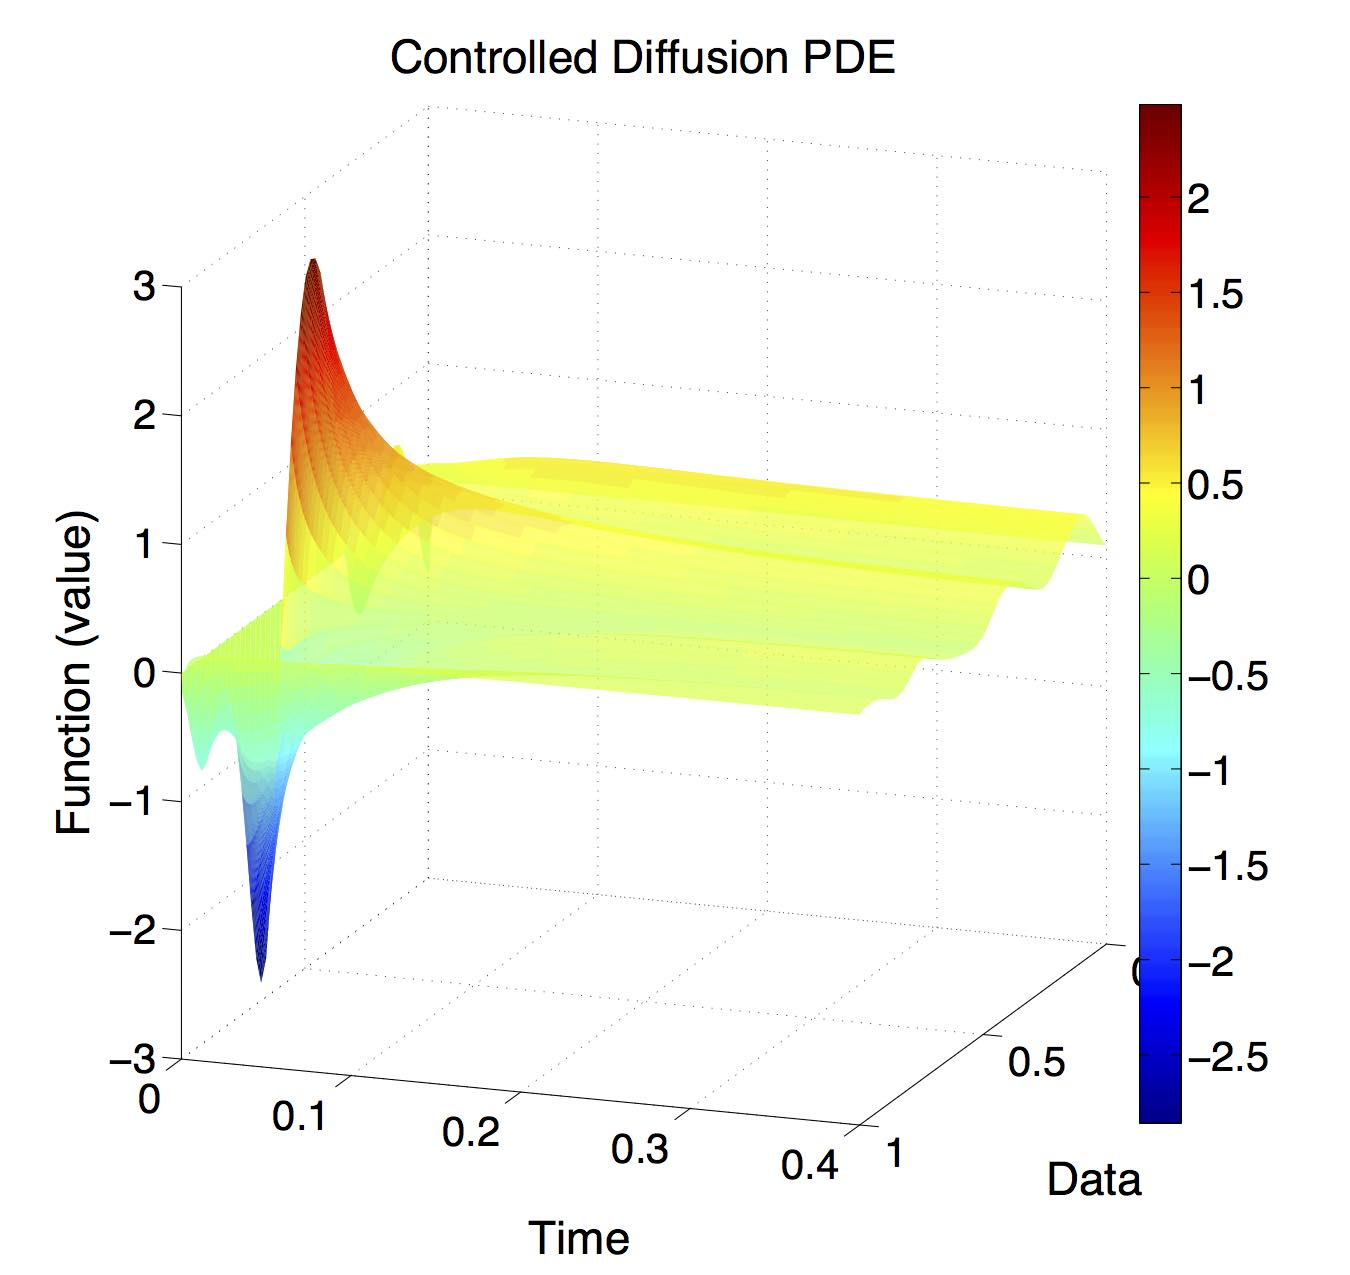
\includegraphics[width=0.5\columnwidth]{controlled_pde_heat.jpg} 
%     \label{fig:controlled_pde}}    
%     \\
    \subfloat[Error in absolute value between controlled pde and $f_{\text{ref}}$. ]{
    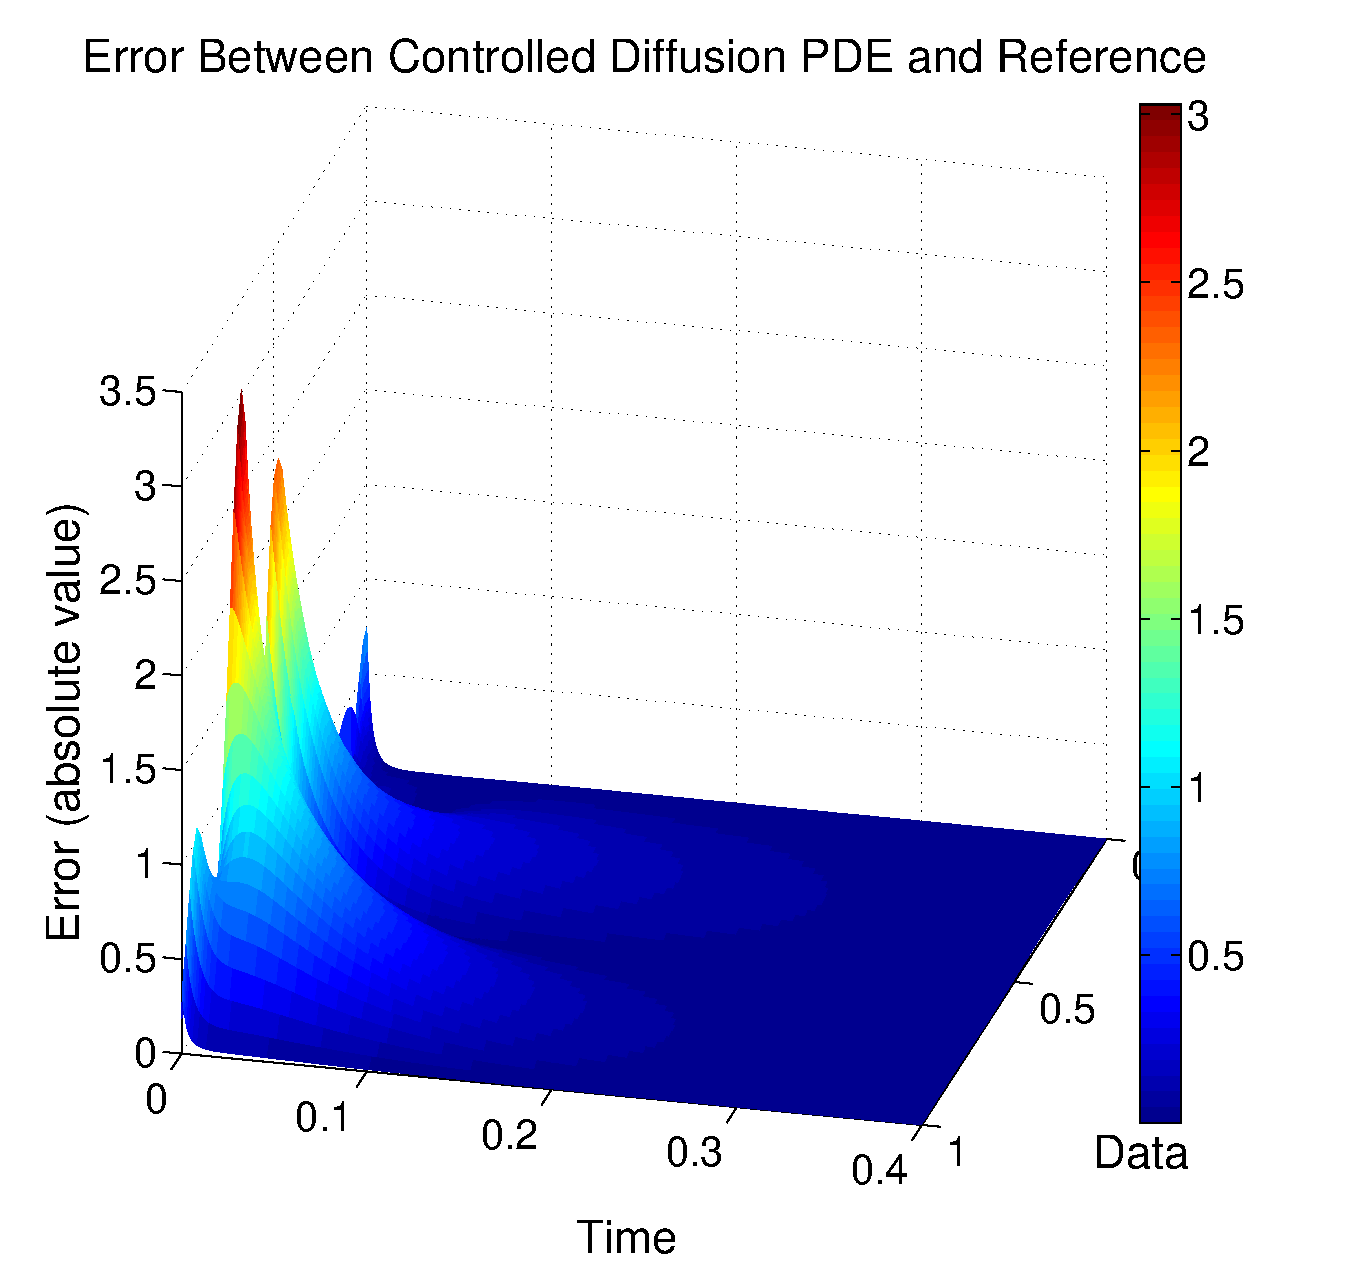
\includegraphics[width=0.45\columnwidth]{controlled_pde_error_heat.pdf} 
    \label{fig:controlled_pde_error} }
    \caption{Demonstration of the control of a linear diffusion equation.}     
\end{figure} 

\section{Conclusion}\label{sec:conclusion}
Machine learning techniques such as Gaussian Process (GP) regression and deep learning are providing increasingly more powerful ways of learning predictive models. For all their power however, since these techniques are limited by the datasets that they are trained with, their predictions are not always reliable when predicting real-world complex spatiotemporally-evolving phenomena with lots of variability; years' worth of weather data cannot be a reliable predictor of current weather, nor can data from one farm directly relate to another. Because of this, when engineering complex cyber-physical systems such as team of mechanically weeding robots, engineers have to think of ways to supplement the predictions of the machine learning models with real measurements. This is not always immediate when one works in the abstract feature spaces utilized in machine learning models. In this tutorial we presented kernel observers and their extension Evolving Gaussian Processes (E-GP), which are formed by embedding a linear dynamical system in the %showed here that despite their abstract nature,
reproducing kernel Hilbert spaces generated by the GP model. The parameters of the linear dynamical system can be trained to approximately predict the evolution. This leads to powerful and generalizable models, as our results demonstrated in predicting solutions to the Navier-Stokes equations. When supplemented with a predict-and-correct strategy, such as a Kalman filter  embedded with the linear dynamical system in the RKHS, the dynamical state of the system can be kept on track with real sensor measurements. This creates a very powerful prediction system that is capable of predicting nonlinear evolution using minimal sensor measurements. We showed that the geometric properties of the linear dynamical system can be utilized to determine sensor numbers and locations. Looking forward, it would interesting to extend the idea to include nonlinear dynamical systems in the feature space, which would improve the capability of the E-GP model. At present, our results on fairly complex datasets demonstrate that feedback with sensors creates a robust monitoring system with the predictions with a simple linear model. The theoretical limits of the tradeoff between improving the model versus increasing the sensing in the context of E-GPs is also an interesting avenue of study. Finally, also we note that deep neural networks have also been applied to the spatiotemporal modeling problem with significant empirical success\cite{tran2015learning}, but because these methods are 1) nonlinear in their parameters, and 2) seem to lack the spatial-encoding properties of some types of kernels, generalizing the analysis considered here for those systems is an interesting open question. As sidebar ``\nameref{sb:featspace}'' indicates, there could be very interesting future work that generalizes the idea of embedding controllers and observers in more advanced features spaces considered in machine learning models. % that  that closing the loop with measurements leads to a sufficiently robust seems  %can be  with   how the weights kernel based regression models are amenable to embedding of dynamical


% that embedding dynamical systems in the f  interpret ability, We demonstrated that the Evolving Gaussian Process model 
%Evolving-Gaussian Processes and Kernel Observers present an 

%\section{Appendix}
This part of the paper presents extra details for the paper. 
\subsection{Proofs of Main Theorems}
% \begin{definition}\label{def:shaded}
% 	\textbf{(Shaded Observation Matrix)} Given $\kernel:\dom\times\dom\to\R$ positive-definite on a domain $\dom$, let $\{\fmapApprox_1(x), \dots, \fmapApprox_{\ncent}(x)\}$ be the set of bases generating an approximate feature map $\fmapApprox:\dom\to\fspaceApprox$, and let
% 	$\sampSet = \sampSetLong$, $x_i\in\dom$. 
% 	Let $\obsMat\in\R^{\nsamp\times\ncent}$ be the observation matrix, where $ \obsMat_{ij} := \fmapApprox_j(x_i)$. For each
% 	row $\obsMat_{(i)} := \left[\begin{smallmatrix}
% 	\fmapApprox_1(x_i) & \cdots & \fmapApprox_{\ncent}(x_i)
% 	\end{smallmatrix}\right]$, define the set 
% 	$\Ind_{(i)} := \{\iota_1^{(i)},\iota_2^{(i)},\dots, \iota_{\ncent_i}^{(i)}\}$ to be the indices in the observation
% 	matrix row $i$ which are nonzero. 
% 	Then if 
% 	%\begin{align}\eqlabel{shaded_cond}
% 	$\bigcup_{i\in\{1,\dots,\nsamp\}} \Ind^{(i)} = \{1,2,\dots, \ncent\}$,
% 	%\end{align}
% 	we denote $\obsMat$ as a \emph{shaded observation matrix} (see Figure \ref{fig:shadeda}).
% \end{definition}
% This definition seems quite abstract, so the following remark considers a more concrete example.
% \begin{remark}\label{rem:shaded}
% 	let $\fmapApprox$ be generated by the dictionary given by $\shCent = \shCentLong$, $c_i\in\dom$. Note that since $\fmapApprox_j(x_i) = \l\fmap(x_i), \fmap(c_j)\r_{\fspace} = \kernel(x_i,c_j)$, $\obsMat$ is the kernel matrix between $\sampSet$ and $\shCent$. For the kernel matrix to be shaded thus implies that there does not exist an atom $\fmap(c_j)$ such that the projections $\l\fmap(x_i),\fmap(c_j)\r_{\fspace}$ vanish for all $x_i$, $1\leq i\leq \nsamp$. Intuitively, the shadedness property requires that the sensor locations $x_i$ are privy to information propagating from every $c_j$. As an example, note that, in principle, for the Gaussian kernel, a single row generates a shaded kernel matrix\footnote{\tiny{However, in this case, the matrix can have many entries that are extremely close to zero, and will probably be very ill-conditioned.}}.  
% \end{remark}
% This condition implies that there does not exist an atom $\fmap(c_j)$ s.t. the projections $\l\fmap(x_i),\fmap(c_j)\r_{\fspaceApprox}$ vanish for all $x_i$, $1\leq i\leq \nsamp$. Intuitively, the shadedness property requires that the sensor locations $x_i$ are privy to information propagating from every atom $c_j$. As an example, note that, in principle, for the Gaussian kernel, a single row generates a shaded kernel matrix\footnote{\tiny{However, in this case, the matrix can have many entries that are extremely close to zero, and will probably be very ill-conditioned.}}. 
%With this definition in place, we can prove the following proposition, which shows that if $\dualopApprox$ has a full-rank Jordan decomposition, a shaded kernel matrix is sufficient to guarantee observability.


% Let $\kernel:\dom\times\dom\to\R$ be a positive definite kernel on a domain $\dom\subset\dom$. 
% Let $C = [c_1,  c_2, \cdots , c_{\ncent}\}$, $c_j\in\dom$ be the centers generating a 
% finite-dimensional covering of the reproducing kernel Hilbert space $\fspaceApprox$ associated to $\kernel(x,y)$, and
% consider the discrete linear system on $\fspaceApprox$ given by
% \begin{align}\eqlabel{hilbert_disc_trans}
%  w_{t+1} = Aw_{t},
% \end{align}
% where $A\in\R^{\ncent\times\ncent}$ has a Jordan decomposition of the form $A = \JorP\JorLa\JorP^{-1}$,
% where $\JorLa$ consists of Jordan blocks along the diagonal, i.e. 
% \begin{align*}
%  \JorLa = 
%  \begin{bmatrix}
%   \JorLa_1 & 0 & 0 &\cdots & 0 \\
%   0 & \JorLa_2 & 0 & \cdots & 0\\
%   \vdots & \vdots & \vdots & \ddots & \vdots\\
%   0 & 0 & 0 & \cdots & \JorLa_{\JorMul}
%  \end{bmatrix}, 
% \end{align*}
% where 
% \begin{align*}
% \JorLa_i := 
%  \begin{bmatrix}
%   \la_i & 1 & 0 & \cdots & 0 & 0\\
%    0 & \la_i & 1 & \cdots & 0 & 0\\
%    \vdots & \vdots & \vdots & \ddots & \vdots & \vdots\\
%    0 & 0 & 0 & \cdots & 0 & \la_i
%  \end{bmatrix}.
% \end{align*}
% Given 
% a set of time instances  $\Tset = \{\tindex_1,\tindex_2,\dots,\tindex_{\otime}\}$, and a set of sampling locations $\sampSet=\sampSetLong$,
% the system \eqref{hilbert_disc_trans} is observable if the kernel matrix $\empK_{ij} := \kernel(x_i,c_j)$ is shaded,
% $\empK^D$, the row vector generated by summing the rows of $\empK$, has all nonzero entries, 
% $\Tset$ has distinct values, and $|\Tset| \geq \ncent$.
Before we prove Proposition \ref{prop:1}, recall that a Jordan decomposition of a matrix $\dualopApprox\in\R^{\ncent\times\ncent}$ with no repeated eigenvalues can be composed of $\JorMul$ Jordan blocks, where $\JorMul$ can be strictly less than $\ncent$. This is in direct contrast to the case where the matrix $\dualopApprox$ has an eigenvalue decomposition, in which case no repeated eigenvalues implies that $\JorMul = \ncent$.  
% \begin{proposition}\label{prop:1}
% 	Given $\kernel:\dom\times\dom\to\R$ positive-definite on a domain $\dom$, let $\{\fmapApprox_1(x), \dots, \fmapApprox_{\ncent}(x)\}$ be the set of bases generating an approximate feature map $\fmapApprox:\dom\to\fspaceApprox$, and let
% 	$\sampSet = \sampSetLong$, $x_i\in\dom$. Consider the discrete linear system on $\fspaceApprox$ given by the evolution and measurement equations \eqref{k_measure}. Suppose that a full-rank Jordan decomposition of $\dualopApprox\in\R^{\ncent\times\ncent}$ of the form $\dualopApprox = \JorP\JorLa\JorP^{-1}$ exists, where $\JorLa = 
% 	\left[\begin{smallmatrix}\JorLa_1 &\cdots & \JorLa_{\JorMul}\end{smallmatrix}\right]$,
% 	and there are no repeated eigenvalues. Then, given a set of time instances  $\Tset = \{\tindex_1,\tindex_2,\dots,\tindex_{\otime}\}$, and a set of sampling locations $\sampSet=\sampSetLong$,
% 	the system \eqref{k_measure} is observable if the observation matrix $\empK_{ij}$ is shaded according to Definition \ref{def:shaded},
% 	% $\empK^D$, the row vector generated by summing the rows of $\empK$, has all nonzero entries, 
% 	$\Tset$ has distinct values, and $|\Tset| \geq \ncent$.
% \end{proposition}
\begin{proof}
 \textbf{(Proposition \ref{prop:1})}
 To begin, consider a system where $\dualopApprox = \JorLa$, with Jordan blocks $\{\JorLa_1, \JorLa_2, \dots, \JorLa_{\JorMul}\}$ along the 
 diagonal. Then $\dualopApprox^{\tindex_i} = \diag(\begin{bmatrix}\JorLa_1^{\tindex_i} & \JorLa_2^{\tindex_i} & \cdots & \JorLa_{\JorMul}^{\tindex_i}\end{bmatrix})$. 
 %The exponentiation of each Jordan block results in upper triangular matrices with linearly independent columns. 
 We have that 
 \begin{align*}
 \Obs_{\Tset} &=
 \underbrace{
 \begin{bmatrix} 
  \empK \dualopApprox^{\tindex_1}\\
  \cdots\\
  \empK \dualopApprox^{\tindex_\otime}.
 \end{bmatrix}}_{\Obs_{\Tset}\in\R^{\nsamp\otime\times\ncent}}
 \end{align*}
 We need to prove that the column rank of $\Obs_{\Tset}$ is $\ncent$, which is not immediately
 obvious since typically $\nsamp \ll \ncent$. To prove the statement, we will show that 
 computing the rank of $\Obs_{\Tset}$ is equivalent to the rank computation of the product of 
 two simple matrices. In what follows,
 we use the notation $\zerosMat{I}{J}$ to denote an $I\times J$ matrix of all zeros. 
 
 In the first step, we write the above matrix as the product of two matrices. 
 Then it can be 
 shown that $\Obs_{\Tset}$ is the product of two block matrices 
 \begin{align*}
 \Obs_{\Tset}  
 &=
 \underbrace{
 \begin{bmatrix}
  \empK   & \cdots & \zerosK\\
  \vdots  & \ddots & \vdots\\
  \zerosK  & \cdots & \empK
 \end{bmatrix}}_{\catempK\in\R^{\nsamp\otime\times\ncent\otime}}
 \underbrace{
 \begin{bmatrix}
  \JorLa_1^{\tindex_1} & \cdots & 0\\
   \vdots & \ddots & \vdots\\
  0 & \cdots & \JorLa_{\JorMul}^{\tindex_1}\\ 
   \hline
   \vdots & \ddots & \vdots\\
   \hline
  \JorLa_1^{\tindex_{\otime}} & \cdots & 0\\
   \vdots & \ddots & \vdots\\
  0 & \cdots & \JorLa_{\JorMul}^{\tindex_\otime}   
 \end{bmatrix}}_{\catdualopC\in\R^{\ncent\otime\times\ncent}}.
\end{align*}
We need to simplify $\catempK$ even further. 
Recall that a matrix's rank is preserved under a product with an invertible matrix. Design a 
matrix of elementary row operations $U\in\R^{\nsamp\times\nsamp}$ such that $\transempK := U\empK$ is a matrix with at least one row vector of nonzeros; this can be achieved by having an elementary matrix that adds rows together. By the shadedness assumption, such a matrix exists. We can write this operation as 
\begin{align*}
 U\empK = 
 \begin{bmatrix}
  \transempK_{11} & \transempK_{12} & \cdots & \transempK_{1\ncent}\\
  \transempK_{21} & \transempK_{22} & \cdots & \transempK_{2\ncent}\\
  \vdots & \vdots & \ddots & \vdots\\
  \transempK_{\nsamp1} & \transempK_{\nsamp2} & \cdots & \transempK_{\nsamp\ncent}.
 \end{bmatrix}
\end{align*}
Without loss of generality, and abusing notation slightly, let this multiplication lead to one nonzero row, with the rest of the elements of the matrix being zero, as 
\begin{align*}
 U\empK = 
 \begin{bmatrix}
  \kernel_{11} & \kernel_{12} & \cdots & \kernel_{1\ncent}\\
  0 & 0 & \cdots & 0\\
  \vdots & \vdots & \ddots & \vdots\\
  0 & 0 & \cdots & 0
 \end{bmatrix}.
\end{align*}
Since elementary matrices are full-rank, we then have that $\Rank(U\empK) = \Rank(\empK)$. 

To analyze the rank of $\Obs_{\Tset}$, we apply these elementary matrices to every $\empK\in\catempK$. To do so, consider the block-diagonal matrix $\bdU\in\R^{\nsamp\otime\times\nsamp\otime}$ with $U\in\R^{\nsamp\times\nsamp}$ along the diagonal, and zeros everywhere else,
i.e.
\begin{align}
 \bdU:= \begin{bmatrix}
  U   & \zerosU & \cdots & \zerosU\\
  \zerosU & U   & \cdots & \zerosU\\
  \vdots  & \vdots  & \ddots & \vdots\\
  \zerosU & \zerosU & \cdots & U
 \end{bmatrix}.
\end{align}
It can be shown that  $\bdU$ is full-rank, i.e. has rank $\nsamp\otime$. Going back to the observability matrix, we have that 
\begin{align*}
 \bdU\Obs_{\Tset} &= \bdU\catempK\catdualopC\\
%  \underbrace{
%  \begin{bmatrix}
%   U   & \zerosU & \cdots & \zerosU\\
%   \zerosU & U   & \cdots & \zerosU\\
%   \vdots  & \vdots  & \ddots & \vdots\\
%   \zerosU & \zerosU & \cdots & U
%  \end{bmatrix}}_{\bdU\in\R^{\nsamp\otime\times\nsamp\otime}}
%  \underbrace{
%  \begin{bmatrix}
%   \empK   & \zerosK & \cdots & \zerosK\\
%   \zerosK & \empK   & \cdots & \zerosK\\
%   \vdots  & \vdots  & \ddots & \vdots\\
%   \zerosK & \zerosK & \cdots & \empK
%  \end{bmatrix}}_{\catempK\in\R^{\nsamp\otime\times\ncent\otime}}
%  \underbrace{
%  \begin{bmatrix}
%   \JorLa_1^{\tindex_1} & 0 & \cdots & 0\\
%   0 & \JorLa_2^{\tindex_1} & \cdots & 0\\
%    \vdots & \vdots & \ddots & \vdots\\
%   0 & 0 & \cdots & \JorLa_{\JorMul}^{\tindex_1}\\ 
%    \hline
%    \vdots & \vdots & \ddots & \vdots\\
%    \hline
%   \JorLa_1^{\tindex_{\otime}} & 0 & \cdots & 0\\
%   0 & \JorLa_2^{\tindex_\otime} & \cdots & 0\\
%    \vdots & \vdots & \ddots & \vdots\\
%   0 & 0 & \cdots & \JorLa_{\JorMul}^{\tindex_\otime}   
%  \end{bmatrix}}_{\catdualopC\in\R^{\ncent\otime\times\ncent}}\\
 &=  
  \underbrace{
  \begin{bmatrix}
  U\empK   & \zerosK & \cdots & \zerosK\\
  \zerosK & U\empK   & \cdots & \zerosK\\
  \vdots  & \vdots  & \ddots & \vdots\\
  \zerosK & \zerosK & \cdots & U\empK
 \end{bmatrix}}_{\bdU\catempK\in\R^{\nsamp\otime\times\ncent\otime}}
 \underbrace{\catdualopC}_{\in\R^{\ncent\otime\times\ncent}},
\end{align*}
since $\zerosU\zerosK = \zerosK$. Due to the fact that $\Rank(\bdU\Obs_{\Tset}) = \Rank(\Obs_{\Tset})$,
we can therefore perform our rank analysis on the simpler matrix $\Rank(\bdU\Obs_{\Tset})$. Note that
\begin{align*}
 U\empK \dualopApprox^{\tindex_j} &=  
 \begin{bmatrix}
  \kernel_{11} & \kernel_{12} & \cdots & \kernel_{1\ncent}\\
  0 & 0 & \cdots & 0\\
  \vdots & \vdots & \ddots & \vdots\\
  0 & 0 & \cdots & 0
 \end{bmatrix}
 \dualopApprox^{\tindex_j}\\
 &= 
 \begin{bmatrix}
  k_{11}\la_1^{\tindex_j} & \binom{\tindex_j}{1}\la_1^{\tindex_j-1} + k_{12}\la_1^{\tindex_j}  & \cdots & k_{1\ncent}\la_{\JorMul}^{\tindex_j}\\
  0 & 0 & \cdots & 0\\
  \vdots & \vdots & \ddots & 0\\
  0 & 0 & \cdots & 0
 \end{bmatrix}.  
\end{align*}
Therefore, following some more elementary row operations encoded by $V\in\R^{\ncent\otime\times\ncent\otime}$, we have that
\begin{align*}
 V \bdU\Obs_{\Tset}
   &= 
   \begin{bmatrix}
    \kernel_{11}\la_1^{\tindex_1} & \cdots & \kernel_{1\ncent}\la_{\JorMul}^{\tindex_1}\\
    \kernel_{11}\la_1^{\tindex_2} & \cdots & \kernel_{1\ncent}\la_{\JorMul}^{\tindex_2}\\
    \vdots & \ddots & 0\\
    \kernel_{11}\la_1^{\tindex_{\otime}} & \cdots 
    & \kernel_{1\ncent}\la_{\JorMul}^{\tindex_{\otime}}\\
    \zerosMat{\ncent(\otime-1)}{1} & \cdots & \zerosMat{\ncent(\otime-1)}{1}
   \end{bmatrix}\\
   &= 
   \begin{bmatrix}
    \boldsymbol{\Phi}\\
    \zerosMat{\ncent(\otime-1)}{\ncent}
   \end{bmatrix}.
\end{align*}
If the individual entries $\kernel_{1i}$ are nonzero, and the Jordan block diagonals have nonzero eigenvalues, the columns of $\boldsymbol\Phi$
become linearly independent. Therefore, if $\otime \geq \ncent$, the column rank of $\Obs_{\Tset}$ is $\ncent$, which results in an observable system.

To extend this proof to matrices $\dualopApprox = \JorP\JorLa\JorP^{-1}$, note that 
\begin{align*}
 \Obs_{\Tset} &= 
 \begin{bmatrix}
  \empK \dualopApprox^{\tindex_1}\\
  \cdots\\
  \empK \dualopApprox^{\tindex_\otime}
 \end{bmatrix}\\
 &=
  \begin{bmatrix}
  \empK \JorP\JorLa^{\tindex_1}\JorP^{-1}\\
  \cdots\\
  \empK \JorP\JorLa^{\tindex_\otime}\JorP^{-1}.
 \end{bmatrix}\\
 &=
 \catempK
 \catJorP
 \catJorLa^t
 \catJorP^{-1},
\end{align*} 
where $\catJorP\in\R^{\ncent\otime\times\ncent\otime}$, $\catJorLa^t\in\R^{\ncent\otime\times\ncent\otime}$, and
$\boldsymbol{\JorP^{-1}}\in\R^{\ncent\otime\times\ncent\otime}$ are the block diagonal matrices associated with the system. 
Since $\catJorP$ is an invertible matrix, the conclusions about the column rank drawn before still hold, and the system is observable. 
\end{proof}


% When the eigenvalues of the system matrix are repeated, it is not enough for $\empK$ to be shaded.
% The next proposition proves a lower bound on the number of sampling locations required. 
% \begin{proposition}\label{prop:2}
%  Suppose that the conditions in Proposition \ref{prop:1} hold, with the relaxation that
%  the Jordan blocks $\left[\begin{smallmatrix}
%                            \JorLa_1 &\cdots & \JorLa_{\JorMul}
%                           \end{smallmatrix}\right]$ may have 
%  repeated eigenvalues (i.e. $\exists \JorLa_i$ and $\JorLa_j$ s.t. $\eval_i = \eval_j$).
% %  Let $\nevals$ be the number of unique eigenvalues of $A$. 
%  Then there exist kernels $\kernel(x,y)$ such that 
%  the lower bound $\minmeas$ on the number of sampling locations $\nsamp$ is given by the cyclic index of $\dualopApprox$.
% \end{proposition}
\begin{proof}
\textbf{(Proposition \ref{prop:2})}
\textbf{By Contrapositive.} We will show that if the number of sampling locations are $ \nsamp=\ell-1 $ (i.e. $ \nsamp < \ell$), then the system is not observable. Pick the Gaussian kernel in the dictionary of atoms framework,
with sampling locations $x_i\in\sampSet$ and centers $c_j\in\shCent$, with the additional 
property that $x_i\neq x_j \forall i,j\in\{1,\dots,\nsamp\}, i\neq j$.
In this case, 
$\empKShadFull$ has $\minmeas-1$ nonzero, linearly independent rows, and can be written as
\begin{align*}
\empKShadFull &= \begin{bmatrix}
k_{11} & k_{12} & \cdots & k_{1\ncent} \\
\vdots & \vdots & \cdots & \vdots \\
k_{(\minmeas-1)1} & k_{(\minmeas-1)2} & \cdots & k_{(\minmeas-1)\ncent} 
\end{bmatrix}.
\end{align*}
Since the cyclic index is $\minmeas$, this implies that at least one eigenvalue, say $\eval$, has $\minmeas$ Jordan 
blocks. 
	%  For concreteness, suppose $\minmeas=2$, and let the size of the blocks be $i\times i$ and $j\times j$. 
	Define indices $j_1, j_2, \dots, j_{\minmeas} \in \{1,2,\dots,\ncent\}$ as the columns corresponding to the leading entries of the $\minmeas$ Jordan blocks corresponding to $\eval$. WLOG, let $j_1 = 1$.
	Using ideas similar to the last proof, we can write the observability matrix as
	\begin{align*}
	\Obs_{\Tset}
	&:= 
	\begin{bmatrix}
	\kernel_{11}\eval^{\tindex_1}  & \cdots & \kernel_{1j_{\minmeas}}\eval^{\tindex_1} & \cdots\\
	\vdots & \ddots &\vdots & \ddots\\
	\kernel_{11}\eval^{\tindex_{\otime}}  & \kernel_{1j_{\minmeas}}\eval^{\tindex_{\otime}} & \cdots\\
	\vdots & \ddots & \vdots & \ddots\\
	\kernel_{(\minmeas-1)1}\eval^{\tindex_1}  \cdots & \kernel_{(\minmeas-1)j_{\minmeas}}\eval^{\tindex_1} & \cdots\\
	\vdots & \ddots &\vdots & \ddots\\
	\kernel_{(\minmeas-1)1}\eval^{\tindex_{\otime}}  & \cdots & \kernel_{(\minmeas-1)j_{\minmeas}}\eval^{\tindex_{\otime}} & \cdots
	\end{bmatrix}.
	\end{align*}
	Define $\evalvec:= \begin{bmatrix}\eval^{\tindex_1} & \eval^{\tindex_2} & \cdots \eval^{\tindex_{\otime}}\end{bmatrix}^T$. 
	Then the above matrix becomes 
	\begin{align*}
	\Obs_{\Tset}
	&:= 
	\begin{bmatrix}
	\kernel_{11}\evalvec  & \cdots & \kernel_{1j_2}\evalvec & \cdots & \kernel_{1j_{\minmeas}}\evalvec & \cdots\\
	\vdots & \ddots & \vdots & \ddots &\vdots & \ddots\\
	\kernel_{(\minmeas-1)1}\evalvec  & \cdots & \kernel_{(\minmeas-1)j_2}\evalvec & \cdots & \kernel_{(\minmeas-1)j_{\minmeas}}\evalvec & \cdots
	\end{bmatrix}.
	\end{align*}
	We need to show that one of the columns above can be written in terms of the others. This is equivalent to solving the linear system
	\begin{align*}
	\begin{bmatrix}
	\kernel_{1j_1}\\
	\kernel_{2j_1}\\
	\vdots\\
	\kernel_{(\minmeas-1)j_1}
	\end{bmatrix}
	%   &=
	%   c_1
	%   \begin{bmatrix}
	%    \kernel_{1j_2}\\
	%    \kernel_{2j_2}\\
	%    \vdots\\
	%    \kernel_{(\minmeas-1)j_2}
	%   \end{bmatrix} 
	%   + \cdots + c_{\minmeas-1}
	%   \begin{bmatrix}
	%    \kernel_{1j_{\minmeas}}\\
	%    \kernel_{2j_{\minmeas}}\\
	%    \vdots\\
	%    \kernel_{(\minmeas-1)j_{\minmeas}}
	%   \end{bmatrix}\\
	&=
	\begin{bmatrix}
	\kernel_{1j_2} & \cdots & \kernel_{1j_{\minmeas}}\\
	\kernel_{2j_2} & \cdots & \kernel_{2j_{\minmeas}}\\
	\vdots & \ddots & \vdots\\
	\kernel_{(\minmeas-1)j_2} & \cdots & \kernel_{(\minmeas-1)j_{\minmeas}}\\
	\end{bmatrix} 
	\begin{bmatrix}
	c_1\\
	c_2\\
	\vdots\\   
	c_{(\minmeas-1)}
	\end{bmatrix}. 
	\end{align*}
	Since the kernel matrix on the RHS is generated from the Gaussian kernel, from \cite{micchelli1984interpolation}, 
	it's known that every principal minor of a Gaussian kernel matrix is invertible, which implies that $\Obs_{\Tset}$ cannot be observable. 
\end{proof}


%Recall that $\minmeas > 1$ implies that there exist spaces $\linspace_i$ s.t. $\R^{\ncent} = \linspace_1\oplus\cdots\oplus\linspace_{\minmeas}$, which induces the decomposition $\fspaceApprox = \fsubspaceC{1}\oplus\cdots\oplus\fsubspaceC{\minmeas}$. 
%% This implies that an initial condition $\initcondf\in\fsubspaceC{\iota}$, remains in $\fsubspaceC{\iota}$ under the action of $\sysopC$, even if the measurement operator $\measop$ corresponds to a shaded matrix $\empK$. 
%As the simplest nontrivial case, consider $\shCent=\{c_1,c_2\}$, $c_i\in\dom$, and pick one sensor location $x_1\in\dom$. Let \eqref{k_measure} be given by 
%$\dualopApprox=\left[\begin{smallmatrix}\eval & 0\\ 0 &\eval\end{smallmatrix}\right]$, $\eval \in\R$ and $ \eval < 0$, and let $\processnoise_{\tindex}$ and $\measnoise_{\tindex}$ be zero. Here, $\minmeas=2$, because there exists no $\linvec\in\R^2$ s.t. $\Span\{\linvec,\dualopApprox\linvec\} = \R^2$. Any initial condition $\initcond$ is an eigenvector for $\dualopApprox$, and thus we get a discrete sequence $\{\initcond, \eval\initcond, \eval^2\initcond,\dots\}$ going to zero along the 1-dimensional subspace generated by $\initcond$. Let $\Tset = \{0, 1\}$ and consider a shaded matrix $\empK = \left[\begin{smallmatrix}\kernel_{11} & \kernel_{12}\end{smallmatrix}\right]$: then the observability matrix is given by $\Obs_{\Tset} = \left[\begin{smallmatrix}\empK^T & (\empK\dualopApprox)^T \end{smallmatrix}\right]^T = \left[\begin{smallmatrix}\kernel_{11} &
%\kernel_{12} \\ \eval\kernel_{11} & \eval\kernel_{12} \end{smallmatrix}\right] = 
%\left[\begin{smallmatrix}\kernelvec_{1}^T &
%\\ \eval\kernelvec_{1}^T\end{smallmatrix}\right]$, which is obviously rank-deficient, and where
%$\left[\begin{smallmatrix}
%\kernel_{11} & \kernel_{12}
%\end{smallmatrix}\right]^T:= \kernelvec_1$. More intuitively, we have that $\Obs_{\Tset}\initcond = 
%\left[\begin{smallmatrix}\l\kernelvec_1, \initcond \r_{\R^2} \\
%\eval\l\kernelvec_1, \initcond \r_{\R^2}\end{smallmatrix}\right]$, which implies that $\kernelvec_1$ doesn't have enough geometric information to recover the initial state. Contrast this with the case when $\dualopApprox=\left[\begin{smallmatrix}\eval & 1\\ 0 &\eval\end{smallmatrix}\right]$; here, $\minmeas=1$, and
%$\Obs_{\Tset} = \left[\begin{smallmatrix}\kernel_{11} &
%\kernel_{12} \\ \eval\kernel_{11} & \kernel_{11} + \eval\kernel_{12} \end{smallmatrix}\right]$, which is full rank for a shaded kernel matrix $\empK$.

% Section \ref{sec:discussion} gives a concrete example to build intuition regarding this lower bound. 
% We now show how to construct a matrix $\measmap$ corresponding to the lower bound $\minmeas$.
% \begin{proposition}
% 	Given the conditions stated in Proposition \ref{prop:2}, it is possible to construct a measurement map $\measmap \in \R^{\minmeas\times\ncent}$ for the system given by \eqref{k_measure}, such that the pair $(\measmap, \dualopApprox)$ is observable.
% \end{proposition}
\begin{proof}
\textbf{(Proposition \ref{prop:3})}
The construction of the measurement map $\measmap$ is based on the rational canonical structure of $\dualopApprox^T$, which decomposes $ \linspace $ into $\dualopApprox^T$-cyclic direct summands such that $\linspace = \linspace_1 \oplus \cdots \oplus \linspace_\minmeas$, where $\minmeas$ is the cyclic index of $\dualopApprox$. Let $\minpolyv_{\linvec}$ be the minimal polynomial (m.p.) of $ \linvec $ (relative to $\dualopApprox^T$): it is then the unique monic polynomial of least degree such that $\minpolyv_{\linvec}(\dualopApprox^T)\linvec=0$. Let $\minpoly_1(\eval)$ be the m.p. of ${\dualopApprox^T}_{|\linspace_1}$: then $\degs(\minpoly_1(\eval)) < \ncent$. By the rational canonical structure theorem \cite{wonham1974linear}, there exists a vector $\widehat{\linvec}_1$, such that $\minpolyv_{\linvec_1}(\eval)=\minpoly_1(\eval)$. Similarly there exists a vector $\widehat{\linvec}_2$, such that $\minpolyv_{\linvec_2}(\eval)=\minpoly_2(\eval)$, where $\minpoly_2(\eval)$, is the minimal polynomial of ${\dualopApprox^T}_{|\linspace_2}$ and so on. Thus we can obtain $\minmeas$ such vectors that form the measurement map $\measmap = [\widehat{\linvec}_1, \widehat{\linvec}_2,\cdots, \widehat{\linvec}_\minmeas]^T$. Construction of these vectors $\widehat{\linvec}_i$, can be simplified by first performing the Jordan decomposition as $ \dualopApprox^T = \JorP\JorLa\JorP^{-1} $. Then the vectors $ \widetilde{\linvec_i},\ i\in \{1,\dots,\minmeas\}$ for $ \JorLa $, can be constructed such that the entries corresponding to the leading entries of Jordan blocks of $ \JorLa_{|\linspace_i} $ are nonzero. Such a construction ensures that the m.p. of vector $ \widetilde{\linvec_i}$ w.r.t $\JorLa_{|\linspace_i}$, is also the corresponding m.p. of 
$\JorLa_{|\linspace_i}$. Finally, the required map can be obtained as $ \measmap = [\widetilde{\linvec_1}, \widetilde{\linvec_2},\dots,\widetilde{\linvec_\minmeas}]^T\JorP^{-1}$.
\end{proof}
%                                                                                                                                                                                    
% 
% The construction provided in the proof of Proposition \ref{prop:3} is utilized in Algorithm \ref{alg:measmap}, which uses the rational canonical structure of $\dualopApprox$ to generate a series of vectors $\linvec_i\in\R^{\ncent}$, whose iterations $\{\linvec_1,\dots,\dualopApprox^{\acycdeg_1-1}\linvec_1,\dots,\linvec_{\minmeas},\dots,\dualopApprox^{\acycdeg_{\minmeas}-1}\linvec_{\minmeas}\}$ generate a basis for $\R^{\ncent}$ (see Section \ref{sec_prelim}). 
% Unfortunately, the measurement map $\measmap$, being an abstract construction unrelated to the kernel, does not directly select $\sampSet$. We will show how to use the measurement map to guide a search for $\sampSet$ in Remark \ref{rem:1}. For now, we state a sufficient condition for observability of a general system. 
% \begin{theorem}\label{thm:1}
% 	Suppose that the conditions in Proposition \ref{prop:1} hold, with the relaxation that
% 	the Jordan blocks $\begin{bmatrix}\JorLa_1 & \JorLa_2 &\cdots & \JorLa_{\JorMul}\end{bmatrix}$ may have 
% 	repeated eigenvalues. Let $\minmeas$ be the cyclic index of $\dualopApprox$.
% 	We define 
% 	\begin{align}\eqlabel{empKShadFull}
% 	\empKShadFull = \left[\begin{smallmatrix}
% 	\empK^{{(1)}^T} & 
% 	\cdots &
% 	\empK^{{(\minmeas)}^T}
% 	\end{smallmatrix}\right]^T
% 	\end{align}
% 	as the \emph{$\minmeas$-shaded matrix} which consists of $\minmeas$ shaded matrices with the property that any subset of
% 	$\minmeas$
% 	columns in the matrix are linearly independent from each
% 	other. Then system \eqref{k_measure} is observable if $\Tset$ has distinct values, and $|\Tset| \geq \ncent$.
% \end{theorem}
\begin{proof}
\textbf{(Theorem \ref{thm:1})}
A cyclic index of $\minmeas$ for this system implies that there exists an eigenvalue $\eval$ that's repeated $\minmeas$
times. We prove the theorem for repeated eigenvalues of dimension 1: the same statement can be proven for repeated eigenvalues for Jordan blocks using the ideas in the proof of Proposition \ref{prop:1}. 
WLOG, let $\empKShadFull$ have $\minmeas$ fully shaded, linearly independent rows, and, assume that the column indices corresponding to this eigenvalue are $\{1,2,\dots,\minmeas\}$. Define 
$\evalvec_i:= \begin{bmatrix}\eval_i^{\tindex_1} & \eval_i^{\tindex_2} & \cdots \eval_i^{\tindex_{\otime}}\end{bmatrix}^T$. Then
	\begin{align*}
	\Obs_{\Tset}
	&:= 
	\begin{bmatrix}
	k_{11} \evalvec_1 & k_{12} \evalvec_2 & \cdots & k_{1\ncent} \evalvec_{\ncent}\\
	\vdots & \vdots & \ddots & \vdots\\
	k_{\minmeas 1} \evalvec_1 & k_{\minmeas 2} \evalvec_2 & \cdots & k_{\minmeas \ncent} \evalvec_{\ncent}
	\end{bmatrix}.
	\end{align*}
	Let $\evalvec_1 = \evalvec_2 = \cdots \evalvec_{\minmeas} := \evalvec$. 
	Focusing on these first $\minmeas$ columns of this matrix, this implies that
	we need to find constants $c_1,c_2,\dots, c_{\minmeas-1}$ such that
	\begin{align*}
	\begin{bmatrix}
	k_{11}\\
	\vdots\\
	k_{\minmeas 1}
	\end{bmatrix}
	&= 
	c_1 
	\begin{bmatrix}
	k_{12}\\
	\vdots\\
	k_{\minmeas 2}
	\end{bmatrix}
	+ \cdots + 
	c_{\minmeas-1} 
	\begin{bmatrix}
	k_{1\minmeas}\\   
	\vdots\\
	k_{\minmeas \minmeas} 
	\end{bmatrix}.
	\end{align*}
	However, these columns are linearly independent by assumption, and thus no such constants exist, implying that $\Obs_{\Tset}$ is observable. 
\end{proof}
While Theorem \ref{thm:1} is a quite general result, the condition that any $\minmeas$ columns of $\empKShadFull$ be linearly independent is a very stringent condition. 
One scenario where this condition can be met with minimal measurements is in the case when the feature map $\fmapApprox(x)$ is generated by a dictionary of atoms with the Gaussian RBF kernel evaluated at sampling locations $\sampSetLong$ according to \eqref{fmap_dict}, where $x_i\in\dom\subset\R^d$, and $x_i$ are sampled from a non-degenerate probability distribution on $\dom$ such as the uniform distribution. For a semi-deterministic approach, when the dynamics matrix $\dualopApprox$ is block-diagonal, we can utilize a simple heuristic:
\begin{remark}\label{rem:1}
	Let $\dom$ be compact, $\shCent = \shCentLong$, $c_i\in\dom$, and let the approximate feature map be defined by \eqref{fmap_dict}. Consider the system \eqref{k_measure} with $\dualopApprox=\JorLa$, and let $\Tset = \{0,1,\dots,\ncent-1\}$. Then the measurement map $\measmap$'s values lie in $\{0, 1\}$; in particular, each row $\measmap^{(j)}$, $j\in\{1,\dots,\minmeas\}$, corresponds to a subspace $\fsubspaceApprox{j}$, generated by a subset of centers $\shCent^{(j)}\subset\shCent$. Generate samples $x_i^{(j)}$ to create a kernel matrix $\empK^{(j)}$ that is shaded only with respect to centers $\shCent^{(j)}$. Once this is done, move on to the next subspace $\fsubspaceApprox{j+1}$. When all $\minmeas$ rows of $\measmap$ are accounted for, construct the matrix $\empKShadFull$ as in \eqref{empKShadFull}. Then the resulting system $(\empKShadFull, \dualopApprox)$ is observable. 
\end{remark}
This heuristic is formalized in Algorithm 2. Note that in practice, the matrix $\dualopApprox$ needs to be inferred from measurements of the process $f_{\tindex}$. If no assumptions are placed on $\dualopApprox$, it's clear that at least $\ncent$ sensors are required for the system identification phase. Future work will study the precise conditions under which system identification is possible with less than $\ncent$ sensors.
\begin{figure}[t!]
	\begin{algorithm}[H]
		\caption{Measurement Map $\measmap$}
		\label{alg:measmap}
		\begin{algorithmic}
			\begin{footnotesize} 
				\STATE {\bfseries Input:} $\dualopApprox\in\R^{\ncent\times\ncent}$
				\STATE Compute Frobenius canonical form, such that $ \FrobC  = \FrobP^{-1} \dualopApprox^T\FrobP$. Set $\FrobC_0:=\FrobC$, and
				$\ncent_0:=\ncent$. 
				%           Obtain subspaces 
				%           $\linspace_i\subset\R^{\ncent}$ s.t. $\R^{\ncent} = \linspace_1\oplus\cdots\oplus\linspace_{\minmeas}$.
				\FOR{$i=1$ {\bfseries to} $\minmeas$}
				\STATE Obtain MP $\minpoly_i(\eval)$ of $\FrobC_{i-1}$. 
				This returns associated indices $\mmapInd{i}\subset\{1,2,\dots,\ncent_{i-1}\}$. 
				%             \STATE Use $\mmapInd{i}$ to select submatrix $\widetilde{\FrobP}_i$, where an index $j\in\mmapInd{i}$ 
				%                    indicates selection of the row and column associated to $j$.
				\STATE Construct vector $\linvec_i \in \R^{\ncent}$ such that 
				$\minpolyv_{\linvec_i}(\eval)=\minpoly_{i}(\eval)$ .
				\STATE Use indices $\{1,2,\dots,\ncent_{i-1}\}\setminus\mmapInd{i}$ to select matrix $\FrobC_i$. Set 
				$\ncent_i:= |\{1,2,\dots,\ncent_{i-1}\}\setminus\mmapInd{i}|$
				\ENDFOR
				\STATE Compute $ \premeasmap = [\linvec_1^T, \linvec_2^T,...,\linvec_{\minmeas}^T]^T$
				\STATE {\bfseries Output:} $ \measmap =\premeasmap\FrobP^{-1}  $
			\end{footnotesize}
		\end{algorithmic}
	\end{algorithm} 
\end{figure}
\begin{figure}[t!]
	\begin{algorithm}[H]
		\caption{Sampling locations set $ \sampSet $}
		\label{alg:samples}
		\begin{algorithmic}
			\begin{footnotesize}	
				\STATE {\bfseries Input:} $ \dualopApprox =\FrobC $, lower bound $\minmeas$
				%		\STATE Check $k=\max_i \nu(\lambda_i)$
				\STATE Decompose $ \FrobC $ to generate invariant subspaces $ \fsubspaceC{j} $, $ j\in \{1,2,\dots,\minmeas\} $ (see section \ref{sec_prelim})
				\FOR{$j=1$ {\bfseries to} $\minmeas$}
				\STATE Obtain centers $\shCent^{(j)}$ w.r.t subspace $ \fsubspaceC{j} $,
				\STATE Generate samples $x_i^{(j)}$ to create a kernel matrix $\empK^{(j)}$ that is shaded only with respect to centers $\shCent^{(j)}$
				\ENDFOR
				\STATE {\bfseries Output:} Sampling locations set  $\sampSet =\{x^{(1)}, x^{(2)}\cdots,x^{(l)}\} $.
			\end{footnotesize}		
		\end{algorithmic}
	\end{algorithm}
\end{figure}
\begin{proof}
	\textbf{(Theorem \ref{thm:r1})}
	For each random sample, the probability that it lies within the $ \epsilon- $shaded region of a particular center $ c_j \in \shCent_\rands$
	is at least $ p_{\e} $. The series of random samples can be considered as Bernoulli trials in which $p_{\e}$ is the probability of a successful outcome. Note this is assuming worst case scenario that the intersection between any two $ \epsilon $-shaded region of centers belonging to the set  $ \shCent_\rands $ is empty. Observability for the pair $ (\empK, \dualopApprox) $ is achieved after $ \rands  $ successful outcomes are obtained because each success ensures a row vector with non-zero entry corresponding to the leading entry of the Jordan block. 
	
	Let $ X_1, X_2, \dots, X_\nsamp $ be i.i.d. random variables whose common distribution is the Bernoulli distribution with parameter $p_{\e}$. The random variable $ X = X_1 + X_2+ \dots+ X_\nsamp $ denotes the number of success after $ \nsamp $ random samples. Since each $ X_i $ has the Bernoulli distribution, $ X $ will have binomial distribution, 
	\begin{equation*}
	P(X=h) = {\nsamp \choose h}p_{\e}^h (1-p_{\e})^{\nsamp-h},
	\end{equation*}
	in which $ h  $ is the number of success. The expectation of the binomial distribution, that is the expected number of success is $ Np_{\e} $, and thus the expected number of trials required will be $ N = \rands/p_{\e}$.
\end{proof}
\begin{proof}
	\textbf{(Theorem \ref{thm:r2})}
	The random variable $ X $ from the proof of Theorem 1 has a binomial distribution, which enables the application of a Chernoff-type bound on its tail probabilities. A well known result  on multiplicative Chernoff bound \cite{motwani2010randomized} is directly applied to establish this Theorem. If $ X $ is binomially distributed, $ \delta \in (0,1] $, and $ \meanDist = \mathbb{E}[X] $, then $ P[X\leq(1-\delta)\meanDist] \leq \exp(-\meanDist \delta^2/2) $, in which we let $ \delta = 1-\frac{\rands}{\nsamp p_{\e}}$.  The expression in the exponent can be simplified to $ -\frac{1}{2}\nsamp p_{\e}+\rands - \frac{\rands^2}{2\nsamp p_{\e}} $, using $ \meanDist = \nsamp p_{\e} $. Note that $ e^{\frac{-\rands^2}{2\nsamp p_{\e}}} \leq 1$. This implies that,
	\begin{equation*}
	\exp(-\meanDist \delta^2/2) =  e^{-\frac{1}{2}(\nsamp p_{\e}-2\rands)}.e^{\frac{-\rands^2}{2\nsamp p_{\e}}}\leq e^{-\frac{1}{2}(\nsamp p_{\e}-2\rands)}
	\end{equation*}
	Note, $ (1-\delta)\mu = \rands $, hence we obtain that $ P[X\leq\rands] \leq e^{-\frac{1}{2}(\nsamp p_{\e}-2\rands)}. $
\end{proof}
 \begin{figure}[t!]
 	\centering
 	\begin{algorithm}[H]
 		\caption{Kernel Observer (Transition Learning)}
 		\label{alg:egp_trans}
 		\begin{algorithmic}
 			\begin{footnotesize}
 				\STATE {\bfseries Input:} Kernel $\kernel$, basis centers $\shCent$, final time 
 				step $\ftime$. 
 				\WHILE{$\tindex \leq \ftime$}
 				\STATE $1)$ Sample data $\{y^i_{\tindex}\}_{i=1}^{\ncent}$ from $f_{\tindex}$. 
 				\STATE $2)$ Estimate $\estweight_\tindex$ via standard kernel inference procedure. 
 				\STATE $3)$ Store weights $\estweight_\tindex$ in matrix $\W\in\R^{\ncent\times \ftime}$.
 				\ENDWHILE
 				\STATE To infer $\dualopApprox$, define matrix $\Phi = \W^T\W$. Then:
 				\FOR{$i=1$ {\bfseries to} $\ncent$}
 				\STATE At step $i$, solve system
 				\begin{align}
 				\dualopApprox^{(i)} = \left(\left(\Phi + \la I\right)^{-1}(\W^T\W^{(i)})\right)^T,
 				\end{align}
 				where $\dualopApprox^{(i)}$, and $\W^{(i)}$ are the $i$th columns of $\dualopApprox$ and $\W^{(i)}$ respectively. 
 				\ENDFOR
 				\STATE Compute the covariance matrix  $\estcontrolop$ of the observed 
 				weights $\W$. 
 				\STATE {\bfseries Output:} estimated transition matrix $\dualopApprox$, predictive covariance    
 				matrix $\estcontrolop$. 
 			\end{footnotesize}
 		\end{algorithmic}
 	\end{algorithm}
 	\vspace{-0.3in}
 \end{figure}
 \begin{figure}[t!]
 	\begin{algorithm}[H]
 		\caption{Kernel Observer (Monitoring and Prediction)}
 		\label{alg:egp_inf}
 		\begin{algorithmic}
 			\begin{footnotesize}
 				\STATE {\bfseries Input:} Kernel $\kernel$, basis centers $\shCent$, 
 				estimated system matrix $\dualopApprox$, estimated covariance matrix $\estcontrolop$.
 				\STATE {\bfseries Compute Observation Matrix:} Compute the cyclic index $\minmeas$ of $\dualopApprox$, and compute $\empK$.
 				\STATE {\bfseries Initialize Observer:} Use $\dualopApprox$, $\estcontrolop$, and $\empK$ to initialize a state-observer (e.g. Kalman filter (KF)) on $\fspaceApprox$.
 				\WHILE{ measurements available }   
 				\STATE 1) Sample data $\{y^i_{\tindex}\}_{i=1}^{\nsamp}$ from $f_{\tindex}$.
 				\STATE 2) Propagate KF estimate $\estweight_{\tindex}$ 
 				forward to time $\tindex+1$, correct using measurement feedback with $\{y^i_{\tindex+1}\}_{i=1}^{\nsamp}$. 
 				\STATE 3) Output predicted function $\widehat{f}_{\tindex+1}$ of KF.
 				\ENDWHILE   
 			\end{footnotesize}
 		\end{algorithmic}
 	\end{algorithm}
 	\vspace{-0.2in}
 \end{figure}
\begin{figure}[tbh]
 \begin{algorithm}[H]
   \caption{Kernel Controller}
   \label{alg:egp_control}
\begin{algorithmic}
\begin{footnotesize}
   \STATE {\bfseries Input:} Kernel $\kernel$, basis points $\shCent$,
   estimated system matrix $\estsysop$, estimated covariance matrix $\estcontrolop$, and function $f_{\text{ref}}$ 
   to drive initial function to.    
   \STATE {\bfseries Initialize Observer:} (see Algorithm \ref{alg:egp_inf}). 
   \STATE {\bfseries Initialize Controller:} Use Jordan decomposition of $\estsysop$ to obtain  no. of control locations $\controlCent$, compute kernel matrix $\empKCD\in\R^{\ncontrol\times\ncent}$ between $\controlCent$ and $\shCent$, and initialize controller (e.g. LQR) utilizing $(\estsysop, \estcontrolop)$.
   \WHILE{ measurements available }   
     \STATE 1) Sample data $\{y^i_k\}_{i=1}^{\nsamp}$ from $f(x,\tindex)$.    
     \STATE 2) Utilize observer to estimate $\estweight_{\tindex+1}$.
     \STATE 3) Use $\estweight_{\tindex+1}$ and $f_{\text{ref}}$ as input to controller to get feedback. 
   \ENDWHILE   
\end{footnotesize}
\end{algorithmic}
\end{algorithm}
\vspace{-0.2in}
\end{figure}


\section{Software}
To facilitate implementation of the material presented in this paper we have made an open source code repository. A MATLAB version is available at \url{http://daslab.illinois.edu/software.html} or at \url{https://github.com/hkingravi/FunctionObservers} with examples and documentation. In addition, a Python version is available on GitHub at \url{https://github.com/hkingravi/funcobspy}.

\section{ACKNOWLEDGMENTS}
The work presented was supported in part by AFOSR \#FA9550-15-1-0146, %NSF SBIR \#1820332, 
and USDA/NSF CPS grant 2018-67007-28379, and USDA/NSF NRI grant 2019-67021-28989.  We thank EarthSense Inc. (www.earthsense.co) for providing us approval to use Figures \ref{fig:cps} and \ref{fig:terrasentia}. The authors also thank Prof. Stephen Long, Prof. Carl Bernacchi, Prof. Michael Gore, and Prof. Edward Buckler on insights about the phenotyping bottleneck and simulation of plants (\textit{crops-in-silico}), Prof. Adam Davis on inputs on the herbicide-resistant weed crisis, and Prof. Sarah Lovell and Dr. Chinmay Soman on sustainable agricultural production systems and perennial polycultures. We also thank the members of the UIUC Center for Digital Agriculture for their inputs.

%\section{Appendix}
This part of the paper presents extra details for the paper. 
\subsection{Proofs of Main Theorems}
% \begin{definition}\label{def:shaded}
% 	\textbf{(Shaded Observation Matrix)} Given $\kernel:\dom\times\dom\to\R$ positive-definite on a domain $\dom$, let $\{\fmapApprox_1(x), \dots, \fmapApprox_{\ncent}(x)\}$ be the set of bases generating an approximate feature map $\fmapApprox:\dom\to\fspaceApprox$, and let
% 	$\sampSet = \sampSetLong$, $x_i\in\dom$. 
% 	Let $\obsMat\in\R^{\nsamp\times\ncent}$ be the observation matrix, where $ \obsMat_{ij} := \fmapApprox_j(x_i)$. For each
% 	row $\obsMat_{(i)} := \left[\begin{smallmatrix}
% 	\fmapApprox_1(x_i) & \cdots & \fmapApprox_{\ncent}(x_i)
% 	\end{smallmatrix}\right]$, define the set 
% 	$\Ind_{(i)} := \{\iota_1^{(i)},\iota_2^{(i)},\dots, \iota_{\ncent_i}^{(i)}\}$ to be the indices in the observation
% 	matrix row $i$ which are nonzero. 
% 	Then if 
% 	%\begin{align}\eqlabel{shaded_cond}
% 	$\bigcup_{i\in\{1,\dots,\nsamp\}} \Ind^{(i)} = \{1,2,\dots, \ncent\}$,
% 	%\end{align}
% 	we denote $\obsMat$ as a \emph{shaded observation matrix} (see Figure \ref{fig:shadeda}).
% \end{definition}
% This definition seems quite abstract, so the following remark considers a more concrete example.
% \begin{remark}\label{rem:shaded}
% 	let $\fmapApprox$ be generated by the dictionary given by $\shCent = \shCentLong$, $c_i\in\dom$. Note that since $\fmapApprox_j(x_i) = \l\fmap(x_i), \fmap(c_j)\r_{\fspace} = \kernel(x_i,c_j)$, $\obsMat$ is the kernel matrix between $\sampSet$ and $\shCent$. For the kernel matrix to be shaded thus implies that there does not exist an atom $\fmap(c_j)$ such that the projections $\l\fmap(x_i),\fmap(c_j)\r_{\fspace}$ vanish for all $x_i$, $1\leq i\leq \nsamp$. Intuitively, the shadedness property requires that the sensor locations $x_i$ are privy to information propagating from every $c_j$. As an example, note that, in principle, for the Gaussian kernel, a single row generates a shaded kernel matrix\footnote{\tiny{However, in this case, the matrix can have many entries that are extremely close to zero, and will probably be very ill-conditioned.}}.  
% \end{remark}
% This condition implies that there does not exist an atom $\fmap(c_j)$ s.t. the projections $\l\fmap(x_i),\fmap(c_j)\r_{\fspaceApprox}$ vanish for all $x_i$, $1\leq i\leq \nsamp$. Intuitively, the shadedness property requires that the sensor locations $x_i$ are privy to information propagating from every atom $c_j$. As an example, note that, in principle, for the Gaussian kernel, a single row generates a shaded kernel matrix\footnote{\tiny{However, in this case, the matrix can have many entries that are extremely close to zero, and will probably be very ill-conditioned.}}. 
%With this definition in place, we can prove the following proposition, which shows that if $\dualopApprox$ has a full-rank Jordan decomposition, a shaded kernel matrix is sufficient to guarantee observability.


% Let $\kernel:\dom\times\dom\to\R$ be a positive definite kernel on a domain $\dom\subset\dom$. 
% Let $C = [c_1,  c_2, \cdots , c_{\ncent}\}$, $c_j\in\dom$ be the centers generating a 
% finite-dimensional covering of the reproducing kernel Hilbert space $\fspaceApprox$ associated to $\kernel(x,y)$, and
% consider the discrete linear system on $\fspaceApprox$ given by
% \begin{align}\eqlabel{hilbert_disc_trans}
%  w_{t+1} = Aw_{t},
% \end{align}
% where $A\in\R^{\ncent\times\ncent}$ has a Jordan decomposition of the form $A = \JorP\JorLa\JorP^{-1}$,
% where $\JorLa$ consists of Jordan blocks along the diagonal, i.e. 
% \begin{align*}
%  \JorLa = 
%  \begin{bmatrix}
%   \JorLa_1 & 0 & 0 &\cdots & 0 \\
%   0 & \JorLa_2 & 0 & \cdots & 0\\
%   \vdots & \vdots & \vdots & \ddots & \vdots\\
%   0 & 0 & 0 & \cdots & \JorLa_{\JorMul}
%  \end{bmatrix}, 
% \end{align*}
% where 
% \begin{align*}
% \JorLa_i := 
%  \begin{bmatrix}
%   \la_i & 1 & 0 & \cdots & 0 & 0\\
%    0 & \la_i & 1 & \cdots & 0 & 0\\
%    \vdots & \vdots & \vdots & \ddots & \vdots & \vdots\\
%    0 & 0 & 0 & \cdots & 0 & \la_i
%  \end{bmatrix}.
% \end{align*}
% Given 
% a set of time instances  $\Tset = \{\tindex_1,\tindex_2,\dots,\tindex_{\otime}\}$, and a set of sampling locations $\sampSet=\sampSetLong$,
% the system \eqref{hilbert_disc_trans} is observable if the kernel matrix $\empK_{ij} := \kernel(x_i,c_j)$ is shaded,
% $\empK^D$, the row vector generated by summing the rows of $\empK$, has all nonzero entries, 
% $\Tset$ has distinct values, and $|\Tset| \geq \ncent$.
Before we prove Proposition \ref{prop:1}, recall that a Jordan decomposition of a matrix $\dualopApprox\in\R^{\ncent\times\ncent}$ with no repeated eigenvalues can be composed of $\JorMul$ Jordan blocks, where $\JorMul$ can be strictly less than $\ncent$. This is in direct contrast to the case where the matrix $\dualopApprox$ has an eigenvalue decomposition, in which case no repeated eigenvalues implies that $\JorMul = \ncent$.  
% \begin{proposition}\label{prop:1}
% 	Given $\kernel:\dom\times\dom\to\R$ positive-definite on a domain $\dom$, let $\{\fmapApprox_1(x), \dots, \fmapApprox_{\ncent}(x)\}$ be the set of bases generating an approximate feature map $\fmapApprox:\dom\to\fspaceApprox$, and let
% 	$\sampSet = \sampSetLong$, $x_i\in\dom$. Consider the discrete linear system on $\fspaceApprox$ given by the evolution and measurement equations \eqref{k_measure}. Suppose that a full-rank Jordan decomposition of $\dualopApprox\in\R^{\ncent\times\ncent}$ of the form $\dualopApprox = \JorP\JorLa\JorP^{-1}$ exists, where $\JorLa = 
% 	\left[\begin{smallmatrix}\JorLa_1 &\cdots & \JorLa_{\JorMul}\end{smallmatrix}\right]$,
% 	and there are no repeated eigenvalues. Then, given a set of time instances  $\Tset = \{\tindex_1,\tindex_2,\dots,\tindex_{\otime}\}$, and a set of sampling locations $\sampSet=\sampSetLong$,
% 	the system \eqref{k_measure} is observable if the observation matrix $\empK_{ij}$ is shaded according to Definition \ref{def:shaded},
% 	% $\empK^D$, the row vector generated by summing the rows of $\empK$, has all nonzero entries, 
% 	$\Tset$ has distinct values, and $|\Tset| \geq \ncent$.
% \end{proposition}
\begin{proof}
 \textbf{(Proposition \ref{prop:1})}
 To begin, consider a system where $\dualopApprox = \JorLa$, with Jordan blocks $\{\JorLa_1, \JorLa_2, \dots, \JorLa_{\JorMul}\}$ along the 
 diagonal. Then $\dualopApprox^{\tindex_i} = \diag(\begin{bmatrix}\JorLa_1^{\tindex_i} & \JorLa_2^{\tindex_i} & \cdots & \JorLa_{\JorMul}^{\tindex_i}\end{bmatrix})$. 
 %The exponentiation of each Jordan block results in upper triangular matrices with linearly independent columns. 
 We have that 
 \begin{align*}
 \Obs_{\Tset} &=
 \underbrace{
 \begin{bmatrix} 
  \empK \dualopApprox^{\tindex_1}\\
  \cdots\\
  \empK \dualopApprox^{\tindex_\otime}.
 \end{bmatrix}}_{\Obs_{\Tset}\in\R^{\nsamp\otime\times\ncent}}
 \end{align*}
 We need to prove that the column rank of $\Obs_{\Tset}$ is $\ncent$, which is not immediately
 obvious since typically $\nsamp \ll \ncent$. To prove the statement, we will show that 
 computing the rank of $\Obs_{\Tset}$ is equivalent to the rank computation of the product of 
 two simple matrices. In what follows,
 we use the notation $\zerosMat{I}{J}$ to denote an $I\times J$ matrix of all zeros. 
 
 In the first step, we write the above matrix as the product of two matrices. 
 Then it can be 
 shown that $\Obs_{\Tset}$ is the product of two block matrices 
 \begin{align*}
 \Obs_{\Tset}  
 &=
 \underbrace{
 \begin{bmatrix}
  \empK   & \cdots & \zerosK\\
  \vdots  & \ddots & \vdots\\
  \zerosK  & \cdots & \empK
 \end{bmatrix}}_{\catempK\in\R^{\nsamp\otime\times\ncent\otime}}
 \underbrace{
 \begin{bmatrix}
  \JorLa_1^{\tindex_1} & \cdots & 0\\
   \vdots & \ddots & \vdots\\
  0 & \cdots & \JorLa_{\JorMul}^{\tindex_1}\\ 
   \hline
   \vdots & \ddots & \vdots\\
   \hline
  \JorLa_1^{\tindex_{\otime}} & \cdots & 0\\
   \vdots & \ddots & \vdots\\
  0 & \cdots & \JorLa_{\JorMul}^{\tindex_\otime}   
 \end{bmatrix}}_{\catdualopC\in\R^{\ncent\otime\times\ncent}}.
\end{align*}
We need to simplify $\catempK$ even further. 
Recall that a matrix's rank is preserved under a product with an invertible matrix. Design a 
matrix of elementary row operations $U\in\R^{\nsamp\times\nsamp}$ such that $\transempK := U\empK$ is a matrix with at least one row vector of nonzeros; this can be achieved by having an elementary matrix that adds rows together. By the shadedness assumption, such a matrix exists. We can write this operation as 
\begin{align*}
 U\empK = 
 \begin{bmatrix}
  \transempK_{11} & \transempK_{12} & \cdots & \transempK_{1\ncent}\\
  \transempK_{21} & \transempK_{22} & \cdots & \transempK_{2\ncent}\\
  \vdots & \vdots & \ddots & \vdots\\
  \transempK_{\nsamp1} & \transempK_{\nsamp2} & \cdots & \transempK_{\nsamp\ncent}.
 \end{bmatrix}
\end{align*}
Without loss of generality, and abusing notation slightly, let this multiplication lead to one nonzero row, with the rest of the elements of the matrix being zero, as 
\begin{align*}
 U\empK = 
 \begin{bmatrix}
  \kernel_{11} & \kernel_{12} & \cdots & \kernel_{1\ncent}\\
  0 & 0 & \cdots & 0\\
  \vdots & \vdots & \ddots & \vdots\\
  0 & 0 & \cdots & 0
 \end{bmatrix}.
\end{align*}
Since elementary matrices are full-rank, we then have that $\Rank(U\empK) = \Rank(\empK)$. 

To analyze the rank of $\Obs_{\Tset}$, we apply these elementary matrices to every $\empK\in\catempK$. To do so, consider the block-diagonal matrix $\bdU\in\R^{\nsamp\otime\times\nsamp\otime}$ with $U\in\R^{\nsamp\times\nsamp}$ along the diagonal, and zeros everywhere else,
i.e.
\begin{align}
 \bdU:= \begin{bmatrix}
  U   & \zerosU & \cdots & \zerosU\\
  \zerosU & U   & \cdots & \zerosU\\
  \vdots  & \vdots  & \ddots & \vdots\\
  \zerosU & \zerosU & \cdots & U
 \end{bmatrix}.
\end{align}
It can be shown that  $\bdU$ is full-rank, i.e. has rank $\nsamp\otime$. Going back to the observability matrix, we have that 
\begin{align*}
 \bdU\Obs_{\Tset} &= \bdU\catempK\catdualopC\\
%  \underbrace{
%  \begin{bmatrix}
%   U   & \zerosU & \cdots & \zerosU\\
%   \zerosU & U   & \cdots & \zerosU\\
%   \vdots  & \vdots  & \ddots & \vdots\\
%   \zerosU & \zerosU & \cdots & U
%  \end{bmatrix}}_{\bdU\in\R^{\nsamp\otime\times\nsamp\otime}}
%  \underbrace{
%  \begin{bmatrix}
%   \empK   & \zerosK & \cdots & \zerosK\\
%   \zerosK & \empK   & \cdots & \zerosK\\
%   \vdots  & \vdots  & \ddots & \vdots\\
%   \zerosK & \zerosK & \cdots & \empK
%  \end{bmatrix}}_{\catempK\in\R^{\nsamp\otime\times\ncent\otime}}
%  \underbrace{
%  \begin{bmatrix}
%   \JorLa_1^{\tindex_1} & 0 & \cdots & 0\\
%   0 & \JorLa_2^{\tindex_1} & \cdots & 0\\
%    \vdots & \vdots & \ddots & \vdots\\
%   0 & 0 & \cdots & \JorLa_{\JorMul}^{\tindex_1}\\ 
%    \hline
%    \vdots & \vdots & \ddots & \vdots\\
%    \hline
%   \JorLa_1^{\tindex_{\otime}} & 0 & \cdots & 0\\
%   0 & \JorLa_2^{\tindex_\otime} & \cdots & 0\\
%    \vdots & \vdots & \ddots & \vdots\\
%   0 & 0 & \cdots & \JorLa_{\JorMul}^{\tindex_\otime}   
%  \end{bmatrix}}_{\catdualopC\in\R^{\ncent\otime\times\ncent}}\\
 &=  
  \underbrace{
  \begin{bmatrix}
  U\empK   & \zerosK & \cdots & \zerosK\\
  \zerosK & U\empK   & \cdots & \zerosK\\
  \vdots  & \vdots  & \ddots & \vdots\\
  \zerosK & \zerosK & \cdots & U\empK
 \end{bmatrix}}_{\bdU\catempK\in\R^{\nsamp\otime\times\ncent\otime}}
 \underbrace{\catdualopC}_{\in\R^{\ncent\otime\times\ncent}},
\end{align*}
since $\zerosU\zerosK = \zerosK$. Due to the fact that $\Rank(\bdU\Obs_{\Tset}) = \Rank(\Obs_{\Tset})$,
we can therefore perform our rank analysis on the simpler matrix $\Rank(\bdU\Obs_{\Tset})$. Note that
\begin{align*}
 U\empK \dualopApprox^{\tindex_j} &=  
 \begin{bmatrix}
  \kernel_{11} & \kernel_{12} & \cdots & \kernel_{1\ncent}\\
  0 & 0 & \cdots & 0\\
  \vdots & \vdots & \ddots & \vdots\\
  0 & 0 & \cdots & 0
 \end{bmatrix}
 \dualopApprox^{\tindex_j}\\
 &= 
 \begin{bmatrix}
  k_{11}\la_1^{\tindex_j} & \binom{\tindex_j}{1}\la_1^{\tindex_j-1} + k_{12}\la_1^{\tindex_j}  & \cdots & k_{1\ncent}\la_{\JorMul}^{\tindex_j}\\
  0 & 0 & \cdots & 0\\
  \vdots & \vdots & \ddots & 0\\
  0 & 0 & \cdots & 0
 \end{bmatrix}.  
\end{align*}
Therefore, following some more elementary row operations encoded by $V\in\R^{\ncent\otime\times\ncent\otime}$, we have that
\begin{align*}
 V \bdU\Obs_{\Tset}
   &= 
   \begin{bmatrix}
    \kernel_{11}\la_1^{\tindex_1} & \cdots & \kernel_{1\ncent}\la_{\JorMul}^{\tindex_1}\\
    \kernel_{11}\la_1^{\tindex_2} & \cdots & \kernel_{1\ncent}\la_{\JorMul}^{\tindex_2}\\
    \vdots & \ddots & 0\\
    \kernel_{11}\la_1^{\tindex_{\otime}} & \cdots 
    & \kernel_{1\ncent}\la_{\JorMul}^{\tindex_{\otime}}\\
    \zerosMat{\ncent(\otime-1)}{1} & \cdots & \zerosMat{\ncent(\otime-1)}{1}
   \end{bmatrix}\\
   &= 
   \begin{bmatrix}
    \boldsymbol{\Phi}\\
    \zerosMat{\ncent(\otime-1)}{\ncent}
   \end{bmatrix}.
\end{align*}
If the individual entries $\kernel_{1i}$ are nonzero, and the Jordan block diagonals have nonzero eigenvalues, the columns of $\boldsymbol\Phi$
become linearly independent. Therefore, if $\otime \geq \ncent$, the column rank of $\Obs_{\Tset}$ is $\ncent$, which results in an observable system.

To extend this proof to matrices $\dualopApprox = \JorP\JorLa\JorP^{-1}$, note that 
\begin{align*}
 \Obs_{\Tset} &= 
 \begin{bmatrix}
  \empK \dualopApprox^{\tindex_1}\\
  \cdots\\
  \empK \dualopApprox^{\tindex_\otime}
 \end{bmatrix}\\
 &=
  \begin{bmatrix}
  \empK \JorP\JorLa^{\tindex_1}\JorP^{-1}\\
  \cdots\\
  \empK \JorP\JorLa^{\tindex_\otime}\JorP^{-1}.
 \end{bmatrix}\\
 &=
 \catempK
 \catJorP
 \catJorLa^t
 \catJorP^{-1},
\end{align*} 
where $\catJorP\in\R^{\ncent\otime\times\ncent\otime}$, $\catJorLa^t\in\R^{\ncent\otime\times\ncent\otime}$, and
$\boldsymbol{\JorP^{-1}}\in\R^{\ncent\otime\times\ncent\otime}$ are the block diagonal matrices associated with the system. 
Since $\catJorP$ is an invertible matrix, the conclusions about the column rank drawn before still hold, and the system is observable. 
\end{proof}


% When the eigenvalues of the system matrix are repeated, it is not enough for $\empK$ to be shaded.
% The next proposition proves a lower bound on the number of sampling locations required. 
% \begin{proposition}\label{prop:2}
%  Suppose that the conditions in Proposition \ref{prop:1} hold, with the relaxation that
%  the Jordan blocks $\left[\begin{smallmatrix}
%                            \JorLa_1 &\cdots & \JorLa_{\JorMul}
%                           \end{smallmatrix}\right]$ may have 
%  repeated eigenvalues (i.e. $\exists \JorLa_i$ and $\JorLa_j$ s.t. $\eval_i = \eval_j$).
% %  Let $\nevals$ be the number of unique eigenvalues of $A$. 
%  Then there exist kernels $\kernel(x,y)$ such that 
%  the lower bound $\minmeas$ on the number of sampling locations $\nsamp$ is given by the cyclic index of $\dualopApprox$.
% \end{proposition}
\begin{proof}
\textbf{(Proposition \ref{prop:2})}
\textbf{By Contrapositive.} We will show that if the number of sampling locations are $ \nsamp=\ell-1 $ (i.e. $ \nsamp < \ell$), then the system is not observable. Pick the Gaussian kernel in the dictionary of atoms framework,
with sampling locations $x_i\in\sampSet$ and centers $c_j\in\shCent$, with the additional 
property that $x_i\neq x_j \forall i,j\in\{1,\dots,\nsamp\}, i\neq j$.
In this case, 
$\empKShadFull$ has $\minmeas-1$ nonzero, linearly independent rows, and can be written as
\begin{align*}
\empKShadFull &= \begin{bmatrix}
k_{11} & k_{12} & \cdots & k_{1\ncent} \\
\vdots & \vdots & \cdots & \vdots \\
k_{(\minmeas-1)1} & k_{(\minmeas-1)2} & \cdots & k_{(\minmeas-1)\ncent} 
\end{bmatrix}.
\end{align*}
Since the cyclic index is $\minmeas$, this implies that at least one eigenvalue, say $\eval$, has $\minmeas$ Jordan 
blocks. 
	%  For concreteness, suppose $\minmeas=2$, and let the size of the blocks be $i\times i$ and $j\times j$. 
	Define indices $j_1, j_2, \dots, j_{\minmeas} \in \{1,2,\dots,\ncent\}$ as the columns corresponding to the leading entries of the $\minmeas$ Jordan blocks corresponding to $\eval$. WLOG, let $j_1 = 1$.
	Using ideas similar to the last proof, we can write the observability matrix as
	\begin{align*}
	\Obs_{\Tset}
	&:= 
	\begin{bmatrix}
	\kernel_{11}\eval^{\tindex_1}  & \cdots & \kernel_{1j_{\minmeas}}\eval^{\tindex_1} & \cdots\\
	\vdots & \ddots &\vdots & \ddots\\
	\kernel_{11}\eval^{\tindex_{\otime}}  & \kernel_{1j_{\minmeas}}\eval^{\tindex_{\otime}} & \cdots\\
	\vdots & \ddots & \vdots & \ddots\\
	\kernel_{(\minmeas-1)1}\eval^{\tindex_1}  \cdots & \kernel_{(\minmeas-1)j_{\minmeas}}\eval^{\tindex_1} & \cdots\\
	\vdots & \ddots &\vdots & \ddots\\
	\kernel_{(\minmeas-1)1}\eval^{\tindex_{\otime}}  & \cdots & \kernel_{(\minmeas-1)j_{\minmeas}}\eval^{\tindex_{\otime}} & \cdots
	\end{bmatrix}.
	\end{align*}
	Define $\evalvec:= \begin{bmatrix}\eval^{\tindex_1} & \eval^{\tindex_2} & \cdots \eval^{\tindex_{\otime}}\end{bmatrix}^T$. 
	Then the above matrix becomes 
	\begin{align*}
	\Obs_{\Tset}
	&:= 
	\begin{bmatrix}
	\kernel_{11}\evalvec  & \cdots & \kernel_{1j_2}\evalvec & \cdots & \kernel_{1j_{\minmeas}}\evalvec & \cdots\\
	\vdots & \ddots & \vdots & \ddots &\vdots & \ddots\\
	\kernel_{(\minmeas-1)1}\evalvec  & \cdots & \kernel_{(\minmeas-1)j_2}\evalvec & \cdots & \kernel_{(\minmeas-1)j_{\minmeas}}\evalvec & \cdots
	\end{bmatrix}.
	\end{align*}
	We need to show that one of the columns above can be written in terms of the others. This is equivalent to solving the linear system
	\begin{align*}
	\begin{bmatrix}
	\kernel_{1j_1}\\
	\kernel_{2j_1}\\
	\vdots\\
	\kernel_{(\minmeas-1)j_1}
	\end{bmatrix}
	%   &=
	%   c_1
	%   \begin{bmatrix}
	%    \kernel_{1j_2}\\
	%    \kernel_{2j_2}\\
	%    \vdots\\
	%    \kernel_{(\minmeas-1)j_2}
	%   \end{bmatrix} 
	%   + \cdots + c_{\minmeas-1}
	%   \begin{bmatrix}
	%    \kernel_{1j_{\minmeas}}\\
	%    \kernel_{2j_{\minmeas}}\\
	%    \vdots\\
	%    \kernel_{(\minmeas-1)j_{\minmeas}}
	%   \end{bmatrix}\\
	&=
	\begin{bmatrix}
	\kernel_{1j_2} & \cdots & \kernel_{1j_{\minmeas}}\\
	\kernel_{2j_2} & \cdots & \kernel_{2j_{\minmeas}}\\
	\vdots & \ddots & \vdots\\
	\kernel_{(\minmeas-1)j_2} & \cdots & \kernel_{(\minmeas-1)j_{\minmeas}}\\
	\end{bmatrix} 
	\begin{bmatrix}
	c_1\\
	c_2\\
	\vdots\\   
	c_{(\minmeas-1)}
	\end{bmatrix}. 
	\end{align*}
	Since the kernel matrix on the RHS is generated from the Gaussian kernel, from \cite{micchelli1984interpolation}, 
	it's known that every principal minor of a Gaussian kernel matrix is invertible, which implies that $\Obs_{\Tset}$ cannot be observable. 
\end{proof}


%Recall that $\minmeas > 1$ implies that there exist spaces $\linspace_i$ s.t. $\R^{\ncent} = \linspace_1\oplus\cdots\oplus\linspace_{\minmeas}$, which induces the decomposition $\fspaceApprox = \fsubspaceC{1}\oplus\cdots\oplus\fsubspaceC{\minmeas}$. 
%% This implies that an initial condition $\initcondf\in\fsubspaceC{\iota}$, remains in $\fsubspaceC{\iota}$ under the action of $\sysopC$, even if the measurement operator $\measop$ corresponds to a shaded matrix $\empK$. 
%As the simplest nontrivial case, consider $\shCent=\{c_1,c_2\}$, $c_i\in\dom$, and pick one sensor location $x_1\in\dom$. Let \eqref{k_measure} be given by 
%$\dualopApprox=\left[\begin{smallmatrix}\eval & 0\\ 0 &\eval\end{smallmatrix}\right]$, $\eval \in\R$ and $ \eval < 0$, and let $\processnoise_{\tindex}$ and $\measnoise_{\tindex}$ be zero. Here, $\minmeas=2$, because there exists no $\linvec\in\R^2$ s.t. $\Span\{\linvec,\dualopApprox\linvec\} = \R^2$. Any initial condition $\initcond$ is an eigenvector for $\dualopApprox$, and thus we get a discrete sequence $\{\initcond, \eval\initcond, \eval^2\initcond,\dots\}$ going to zero along the 1-dimensional subspace generated by $\initcond$. Let $\Tset = \{0, 1\}$ and consider a shaded matrix $\empK = \left[\begin{smallmatrix}\kernel_{11} & \kernel_{12}\end{smallmatrix}\right]$: then the observability matrix is given by $\Obs_{\Tset} = \left[\begin{smallmatrix}\empK^T & (\empK\dualopApprox)^T \end{smallmatrix}\right]^T = \left[\begin{smallmatrix}\kernel_{11} &
%\kernel_{12} \\ \eval\kernel_{11} & \eval\kernel_{12} \end{smallmatrix}\right] = 
%\left[\begin{smallmatrix}\kernelvec_{1}^T &
%\\ \eval\kernelvec_{1}^T\end{smallmatrix}\right]$, which is obviously rank-deficient, and where
%$\left[\begin{smallmatrix}
%\kernel_{11} & \kernel_{12}
%\end{smallmatrix}\right]^T:= \kernelvec_1$. More intuitively, we have that $\Obs_{\Tset}\initcond = 
%\left[\begin{smallmatrix}\l\kernelvec_1, \initcond \r_{\R^2} \\
%\eval\l\kernelvec_1, \initcond \r_{\R^2}\end{smallmatrix}\right]$, which implies that $\kernelvec_1$ doesn't have enough geometric information to recover the initial state. Contrast this with the case when $\dualopApprox=\left[\begin{smallmatrix}\eval & 1\\ 0 &\eval\end{smallmatrix}\right]$; here, $\minmeas=1$, and
%$\Obs_{\Tset} = \left[\begin{smallmatrix}\kernel_{11} &
%\kernel_{12} \\ \eval\kernel_{11} & \kernel_{11} + \eval\kernel_{12} \end{smallmatrix}\right]$, which is full rank for a shaded kernel matrix $\empK$.

% Section \ref{sec:discussion} gives a concrete example to build intuition regarding this lower bound. 
% We now show how to construct a matrix $\measmap$ corresponding to the lower bound $\minmeas$.
% \begin{proposition}
% 	Given the conditions stated in Proposition \ref{prop:2}, it is possible to construct a measurement map $\measmap \in \R^{\minmeas\times\ncent}$ for the system given by \eqref{k_measure}, such that the pair $(\measmap, \dualopApprox)$ is observable.
% \end{proposition}
\begin{proof}
\textbf{(Proposition \ref{prop:3})}
The construction of the measurement map $\measmap$ is based on the rational canonical structure of $\dualopApprox^T$, which decomposes $ \linspace $ into $\dualopApprox^T$-cyclic direct summands such that $\linspace = \linspace_1 \oplus \cdots \oplus \linspace_\minmeas$, where $\minmeas$ is the cyclic index of $\dualopApprox$. Let $\minpolyv_{\linvec}$ be the minimal polynomial (m.p.) of $ \linvec $ (relative to $\dualopApprox^T$): it is then the unique monic polynomial of least degree such that $\minpolyv_{\linvec}(\dualopApprox^T)\linvec=0$. Let $\minpoly_1(\eval)$ be the m.p. of ${\dualopApprox^T}_{|\linspace_1}$: then $\degs(\minpoly_1(\eval)) < \ncent$. By the rational canonical structure theorem \cite{wonham1974linear}, there exists a vector $\widehat{\linvec}_1$, such that $\minpolyv_{\linvec_1}(\eval)=\minpoly_1(\eval)$. Similarly there exists a vector $\widehat{\linvec}_2$, such that $\minpolyv_{\linvec_2}(\eval)=\minpoly_2(\eval)$, where $\minpoly_2(\eval)$, is the minimal polynomial of ${\dualopApprox^T}_{|\linspace_2}$ and so on. Thus we can obtain $\minmeas$ such vectors that form the measurement map $\measmap = [\widehat{\linvec}_1, \widehat{\linvec}_2,\cdots, \widehat{\linvec}_\minmeas]^T$. Construction of these vectors $\widehat{\linvec}_i$, can be simplified by first performing the Jordan decomposition as $ \dualopApprox^T = \JorP\JorLa\JorP^{-1} $. Then the vectors $ \widetilde{\linvec_i},\ i\in \{1,\dots,\minmeas\}$ for $ \JorLa $, can be constructed such that the entries corresponding to the leading entries of Jordan blocks of $ \JorLa_{|\linspace_i} $ are nonzero. Such a construction ensures that the m.p. of vector $ \widetilde{\linvec_i}$ w.r.t $\JorLa_{|\linspace_i}$, is also the corresponding m.p. of 
$\JorLa_{|\linspace_i}$. Finally, the required map can be obtained as $ \measmap = [\widetilde{\linvec_1}, \widetilde{\linvec_2},\dots,\widetilde{\linvec_\minmeas}]^T\JorP^{-1}$.
\end{proof}
%                                                                                                                                                                                    
% 
% The construction provided in the proof of Proposition \ref{prop:3} is utilized in Algorithm \ref{alg:measmap}, which uses the rational canonical structure of $\dualopApprox$ to generate a series of vectors $\linvec_i\in\R^{\ncent}$, whose iterations $\{\linvec_1,\dots,\dualopApprox^{\acycdeg_1-1}\linvec_1,\dots,\linvec_{\minmeas},\dots,\dualopApprox^{\acycdeg_{\minmeas}-1}\linvec_{\minmeas}\}$ generate a basis for $\R^{\ncent}$ (see Section \ref{sec_prelim}). 
% Unfortunately, the measurement map $\measmap$, being an abstract construction unrelated to the kernel, does not directly select $\sampSet$. We will show how to use the measurement map to guide a search for $\sampSet$ in Remark \ref{rem:1}. For now, we state a sufficient condition for observability of a general system. 
% \begin{theorem}\label{thm:1}
% 	Suppose that the conditions in Proposition \ref{prop:1} hold, with the relaxation that
% 	the Jordan blocks $\begin{bmatrix}\JorLa_1 & \JorLa_2 &\cdots & \JorLa_{\JorMul}\end{bmatrix}$ may have 
% 	repeated eigenvalues. Let $\minmeas$ be the cyclic index of $\dualopApprox$.
% 	We define 
% 	\begin{align}\eqlabel{empKShadFull}
% 	\empKShadFull = \left[\begin{smallmatrix}
% 	\empK^{{(1)}^T} & 
% 	\cdots &
% 	\empK^{{(\minmeas)}^T}
% 	\end{smallmatrix}\right]^T
% 	\end{align}
% 	as the \emph{$\minmeas$-shaded matrix} which consists of $\minmeas$ shaded matrices with the property that any subset of
% 	$\minmeas$
% 	columns in the matrix are linearly independent from each
% 	other. Then system \eqref{k_measure} is observable if $\Tset$ has distinct values, and $|\Tset| \geq \ncent$.
% \end{theorem}
\begin{proof}
\textbf{(Theorem \ref{thm:1})}
A cyclic index of $\minmeas$ for this system implies that there exists an eigenvalue $\eval$ that's repeated $\minmeas$
times. We prove the theorem for repeated eigenvalues of dimension 1: the same statement can be proven for repeated eigenvalues for Jordan blocks using the ideas in the proof of Proposition \ref{prop:1}. 
WLOG, let $\empKShadFull$ have $\minmeas$ fully shaded, linearly independent rows, and, assume that the column indices corresponding to this eigenvalue are $\{1,2,\dots,\minmeas\}$. Define 
$\evalvec_i:= \begin{bmatrix}\eval_i^{\tindex_1} & \eval_i^{\tindex_2} & \cdots \eval_i^{\tindex_{\otime}}\end{bmatrix}^T$. Then
	\begin{align*}
	\Obs_{\Tset}
	&:= 
	\begin{bmatrix}
	k_{11} \evalvec_1 & k_{12} \evalvec_2 & \cdots & k_{1\ncent} \evalvec_{\ncent}\\
	\vdots & \vdots & \ddots & \vdots\\
	k_{\minmeas 1} \evalvec_1 & k_{\minmeas 2} \evalvec_2 & \cdots & k_{\minmeas \ncent} \evalvec_{\ncent}
	\end{bmatrix}.
	\end{align*}
	Let $\evalvec_1 = \evalvec_2 = \cdots \evalvec_{\minmeas} := \evalvec$. 
	Focusing on these first $\minmeas$ columns of this matrix, this implies that
	we need to find constants $c_1,c_2,\dots, c_{\minmeas-1}$ such that
	\begin{align*}
	\begin{bmatrix}
	k_{11}\\
	\vdots\\
	k_{\minmeas 1}
	\end{bmatrix}
	&= 
	c_1 
	\begin{bmatrix}
	k_{12}\\
	\vdots\\
	k_{\minmeas 2}
	\end{bmatrix}
	+ \cdots + 
	c_{\minmeas-1} 
	\begin{bmatrix}
	k_{1\minmeas}\\   
	\vdots\\
	k_{\minmeas \minmeas} 
	\end{bmatrix}.
	\end{align*}
	However, these columns are linearly independent by assumption, and thus no such constants exist, implying that $\Obs_{\Tset}$ is observable. 
\end{proof}
While Theorem \ref{thm:1} is a quite general result, the condition that any $\minmeas$ columns of $\empKShadFull$ be linearly independent is a very stringent condition. 
One scenario where this condition can be met with minimal measurements is in the case when the feature map $\fmapApprox(x)$ is generated by a dictionary of atoms with the Gaussian RBF kernel evaluated at sampling locations $\sampSetLong$ according to \eqref{fmap_dict}, where $x_i\in\dom\subset\R^d$, and $x_i$ are sampled from a non-degenerate probability distribution on $\dom$ such as the uniform distribution. For a semi-deterministic approach, when the dynamics matrix $\dualopApprox$ is block-diagonal, we can utilize a simple heuristic:
\begin{remark}\label{rem:1}
	Let $\dom$ be compact, $\shCent = \shCentLong$, $c_i\in\dom$, and let the approximate feature map be defined by \eqref{fmap_dict}. Consider the system \eqref{k_measure} with $\dualopApprox=\JorLa$, and let $\Tset = \{0,1,\dots,\ncent-1\}$. Then the measurement map $\measmap$'s values lie in $\{0, 1\}$; in particular, each row $\measmap^{(j)}$, $j\in\{1,\dots,\minmeas\}$, corresponds to a subspace $\fsubspaceApprox{j}$, generated by a subset of centers $\shCent^{(j)}\subset\shCent$. Generate samples $x_i^{(j)}$ to create a kernel matrix $\empK^{(j)}$ that is shaded only with respect to centers $\shCent^{(j)}$. Once this is done, move on to the next subspace $\fsubspaceApprox{j+1}$. When all $\minmeas$ rows of $\measmap$ are accounted for, construct the matrix $\empKShadFull$ as in \eqref{empKShadFull}. Then the resulting system $(\empKShadFull, \dualopApprox)$ is observable. 
\end{remark}
This heuristic is formalized in Algorithm 2. Note that in practice, the matrix $\dualopApprox$ needs to be inferred from measurements of the process $f_{\tindex}$. If no assumptions are placed on $\dualopApprox$, it's clear that at least $\ncent$ sensors are required for the system identification phase. Future work will study the precise conditions under which system identification is possible with less than $\ncent$ sensors.
\begin{figure}[t!]
	\begin{algorithm}[H]
		\caption{Measurement Map $\measmap$}
		\label{alg:measmap}
		\begin{algorithmic}
			\begin{footnotesize} 
				\STATE {\bfseries Input:} $\dualopApprox\in\R^{\ncent\times\ncent}$
				\STATE Compute Frobenius canonical form, such that $ \FrobC  = \FrobP^{-1} \dualopApprox^T\FrobP$. Set $\FrobC_0:=\FrobC$, and
				$\ncent_0:=\ncent$. 
				%           Obtain subspaces 
				%           $\linspace_i\subset\R^{\ncent}$ s.t. $\R^{\ncent} = \linspace_1\oplus\cdots\oplus\linspace_{\minmeas}$.
				\FOR{$i=1$ {\bfseries to} $\minmeas$}
				\STATE Obtain MP $\minpoly_i(\eval)$ of $\FrobC_{i-1}$. 
				This returns associated indices $\mmapInd{i}\subset\{1,2,\dots,\ncent_{i-1}\}$. 
				%             \STATE Use $\mmapInd{i}$ to select submatrix $\widetilde{\FrobP}_i$, where an index $j\in\mmapInd{i}$ 
				%                    indicates selection of the row and column associated to $j$.
				\STATE Construct vector $\linvec_i \in \R^{\ncent}$ such that 
				$\minpolyv_{\linvec_i}(\eval)=\minpoly_{i}(\eval)$ .
				\STATE Use indices $\{1,2,\dots,\ncent_{i-1}\}\setminus\mmapInd{i}$ to select matrix $\FrobC_i$. Set 
				$\ncent_i:= |\{1,2,\dots,\ncent_{i-1}\}\setminus\mmapInd{i}|$
				\ENDFOR
				\STATE Compute $ \premeasmap = [\linvec_1^T, \linvec_2^T,...,\linvec_{\minmeas}^T]^T$
				\STATE {\bfseries Output:} $ \measmap =\premeasmap\FrobP^{-1}  $
			\end{footnotesize}
		\end{algorithmic}
	\end{algorithm} 
\end{figure}
\begin{figure}[t!]
	\begin{algorithm}[H]
		\caption{Sampling locations set $ \sampSet $}
		\label{alg:samples}
		\begin{algorithmic}
			\begin{footnotesize}	
				\STATE {\bfseries Input:} $ \dualopApprox =\FrobC $, lower bound $\minmeas$
				%		\STATE Check $k=\max_i \nu(\lambda_i)$
				\STATE Decompose $ \FrobC $ to generate invariant subspaces $ \fsubspaceC{j} $, $ j\in \{1,2,\dots,\minmeas\} $ (see section \ref{sec_prelim})
				\FOR{$j=1$ {\bfseries to} $\minmeas$}
				\STATE Obtain centers $\shCent^{(j)}$ w.r.t subspace $ \fsubspaceC{j} $,
				\STATE Generate samples $x_i^{(j)}$ to create a kernel matrix $\empK^{(j)}$ that is shaded only with respect to centers $\shCent^{(j)}$
				\ENDFOR
				\STATE {\bfseries Output:} Sampling locations set  $\sampSet =\{x^{(1)}, x^{(2)}\cdots,x^{(l)}\} $.
			\end{footnotesize}		
		\end{algorithmic}
	\end{algorithm}
\end{figure}
\begin{proof}
	\textbf{(Theorem \ref{thm:r1})}
	For each random sample, the probability that it lies within the $ \epsilon- $shaded region of a particular center $ c_j \in \shCent_\rands$
	is at least $ p_{\e} $. The series of random samples can be considered as Bernoulli trials in which $p_{\e}$ is the probability of a successful outcome. Note this is assuming worst case scenario that the intersection between any two $ \epsilon $-shaded region of centers belonging to the set  $ \shCent_\rands $ is empty. Observability for the pair $ (\empK, \dualopApprox) $ is achieved after $ \rands  $ successful outcomes are obtained because each success ensures a row vector with non-zero entry corresponding to the leading entry of the Jordan block. 
	
	Let $ X_1, X_2, \dots, X_\nsamp $ be i.i.d. random variables whose common distribution is the Bernoulli distribution with parameter $p_{\e}$. The random variable $ X = X_1 + X_2+ \dots+ X_\nsamp $ denotes the number of success after $ \nsamp $ random samples. Since each $ X_i $ has the Bernoulli distribution, $ X $ will have binomial distribution, 
	\begin{equation*}
	P(X=h) = {\nsamp \choose h}p_{\e}^h (1-p_{\e})^{\nsamp-h},
	\end{equation*}
	in which $ h  $ is the number of success. The expectation of the binomial distribution, that is the expected number of success is $ Np_{\e} $, and thus the expected number of trials required will be $ N = \rands/p_{\e}$.
\end{proof}
\begin{proof}
	\textbf{(Theorem \ref{thm:r2})}
	The random variable $ X $ from the proof of Theorem 1 has a binomial distribution, which enables the application of a Chernoff-type bound on its tail probabilities. A well known result  on multiplicative Chernoff bound \cite{motwani2010randomized} is directly applied to establish this Theorem. If $ X $ is binomially distributed, $ \delta \in (0,1] $, and $ \meanDist = \mathbb{E}[X] $, then $ P[X\leq(1-\delta)\meanDist] \leq \exp(-\meanDist \delta^2/2) $, in which we let $ \delta = 1-\frac{\rands}{\nsamp p_{\e}}$.  The expression in the exponent can be simplified to $ -\frac{1}{2}\nsamp p_{\e}+\rands - \frac{\rands^2}{2\nsamp p_{\e}} $, using $ \meanDist = \nsamp p_{\e} $. Note that $ e^{\frac{-\rands^2}{2\nsamp p_{\e}}} \leq 1$. This implies that,
	\begin{equation*}
	\exp(-\meanDist \delta^2/2) =  e^{-\frac{1}{2}(\nsamp p_{\e}-2\rands)}.e^{\frac{-\rands^2}{2\nsamp p_{\e}}}\leq e^{-\frac{1}{2}(\nsamp p_{\e}-2\rands)}
	\end{equation*}
	Note, $ (1-\delta)\mu = \rands $, hence we obtain that $ P[X\leq\rands] \leq e^{-\frac{1}{2}(\nsamp p_{\e}-2\rands)}. $
\end{proof}
 \begin{figure}[t!]
 	\centering
 	\begin{algorithm}[H]
 		\caption{Kernel Observer (Transition Learning)}
 		\label{alg:egp_trans}
 		\begin{algorithmic}
 			\begin{footnotesize}
 				\STATE {\bfseries Input:} Kernel $\kernel$, basis centers $\shCent$, final time 
 				step $\ftime$. 
 				\WHILE{$\tindex \leq \ftime$}
 				\STATE $1)$ Sample data $\{y^i_{\tindex}\}_{i=1}^{\ncent}$ from $f_{\tindex}$. 
 				\STATE $2)$ Estimate $\estweight_\tindex$ via standard kernel inference procedure. 
 				\STATE $3)$ Store weights $\estweight_\tindex$ in matrix $\W\in\R^{\ncent\times \ftime}$.
 				\ENDWHILE
 				\STATE To infer $\dualopApprox$, define matrix $\Phi = \W^T\W$. Then:
 				\FOR{$i=1$ {\bfseries to} $\ncent$}
 				\STATE At step $i$, solve system
 				\begin{align}
 				\dualopApprox^{(i)} = \left(\left(\Phi + \la I\right)^{-1}(\W^T\W^{(i)})\right)^T,
 				\end{align}
 				where $\dualopApprox^{(i)}$, and $\W^{(i)}$ are the $i$th columns of $\dualopApprox$ and $\W^{(i)}$ respectively. 
 				\ENDFOR
 				\STATE Compute the covariance matrix  $\estcontrolop$ of the observed 
 				weights $\W$. 
 				\STATE {\bfseries Output:} estimated transition matrix $\dualopApprox$, predictive covariance    
 				matrix $\estcontrolop$. 
 			\end{footnotesize}
 		\end{algorithmic}
 	\end{algorithm}
 	\vspace{-0.3in}
 \end{figure}
 \begin{figure}[t!]
 	\begin{algorithm}[H]
 		\caption{Kernel Observer (Monitoring and Prediction)}
 		\label{alg:egp_inf}
 		\begin{algorithmic}
 			\begin{footnotesize}
 				\STATE {\bfseries Input:} Kernel $\kernel$, basis centers $\shCent$, 
 				estimated system matrix $\dualopApprox$, estimated covariance matrix $\estcontrolop$.
 				\STATE {\bfseries Compute Observation Matrix:} Compute the cyclic index $\minmeas$ of $\dualopApprox$, and compute $\empK$.
 				\STATE {\bfseries Initialize Observer:} Use $\dualopApprox$, $\estcontrolop$, and $\empK$ to initialize a state-observer (e.g. Kalman filter (KF)) on $\fspaceApprox$.
 				\WHILE{ measurements available }   
 				\STATE 1) Sample data $\{y^i_{\tindex}\}_{i=1}^{\nsamp}$ from $f_{\tindex}$.
 				\STATE 2) Propagate KF estimate $\estweight_{\tindex}$ 
 				forward to time $\tindex+1$, correct using measurement feedback with $\{y^i_{\tindex+1}\}_{i=1}^{\nsamp}$. 
 				\STATE 3) Output predicted function $\widehat{f}_{\tindex+1}$ of KF.
 				\ENDWHILE   
 			\end{footnotesize}
 		\end{algorithmic}
 	\end{algorithm}
 	\vspace{-0.2in}
 \end{figure}
\begin{figure}[tbh]
 \begin{algorithm}[H]
   \caption{Kernel Controller}
   \label{alg:egp_control}
\begin{algorithmic}
\begin{footnotesize}
   \STATE {\bfseries Input:} Kernel $\kernel$, basis points $\shCent$,
   estimated system matrix $\estsysop$, estimated covariance matrix $\estcontrolop$, and function $f_{\text{ref}}$ 
   to drive initial function to.    
   \STATE {\bfseries Initialize Observer:} (see Algorithm \ref{alg:egp_inf}). 
   \STATE {\bfseries Initialize Controller:} Use Jordan decomposition of $\estsysop$ to obtain  no. of control locations $\controlCent$, compute kernel matrix $\empKCD\in\R^{\ncontrol\times\ncent}$ between $\controlCent$ and $\shCent$, and initialize controller (e.g. LQR) utilizing $(\estsysop, \estcontrolop)$.
   \WHILE{ measurements available }   
     \STATE 1) Sample data $\{y^i_k\}_{i=1}^{\nsamp}$ from $f(x,\tindex)$.    
     \STATE 2) Utilize observer to estimate $\estweight_{\tindex+1}$.
     \STATE 3) Use $\estweight_{\tindex+1}$ and $f_{\text{ref}}$ as input to controller to get feedback. 
   \ENDWHILE   
\end{footnotesize}
\end{algorithmic}
\end{algorithm}
\vspace{-0.2in}
\end{figure}


%\section{AUTHOR INFORMATION}
%\mX{Please include a short biography of each author. Please include the mailing address,
%email, telephone number, and fax number of the corresponding author only.}

\clearpage
%\XX{many of hte references have ``gaussian'' rather than ``Gaussian''}
\bibliographystyle{unsrt}
%needs gp_tuotrial
\bibliography{BIB/daslab_all,BIB/daslab_pubs,BIB/ACL_all,BIB/ACL_Publications,BIB/bibtex_database_chowdhary_machine_learning,BIB/cybersees,BIB/Robotics}
%\bibliography{acl_all,daslab_all,daslab_pubs,ACL_Publications}
%\bibliography{gp_tutorial,./BIB_all/ACL_all,./BIB_all/ACL_Publications,./BIB_all/ACL_bef2000,./bibifiles/daslab_pubs,./bibifiles/daslab_all,./bibifiles/controls}

%\begin{thebibliography}{10}
%\bibitem{LT} Available online (last accessed 4/25/16)\\ \url{http://ieeecss.org/sites/ieeecss.org/files/documents/CSMLatex.zip}	
%\bibitem{BIB} Available online (last accessed 4/25/16)\\ \url{https://www.ctan.org/tex-archive/macros/latex/contrib/IEEEtran/bibtex}
%\end{thebibliography}

%\XX{make sure that original publication source of each figure is referenced and acknowledged correctly here}
\processdelayedfloats
\sidebars
%\subsection[Use of Hyphens]{Sidebar: Use of Hyphens}
%\label{sb:UseofHyphens}
%    		
%Note the spelling of these words as single words with no hyphen:  aeroelastic, aeroservoelastic, aimpoint, allpass, axisymmetric, backup, bandpass, bandlimited, bloodstream, breakpoint, buildup, colocated, coprime, countdown, counterclockwise, counterintuitive, counterproductive, crossover, cutoff, deadbeat, deadzone, drivetrain, electromechanical, feedback, feedforward, feedthrough, flyby, gearbox, geartrain, handheld, hardwired, highpass, ingoing, inline, interagent, interarrival, interrelated, liftoff, lightweight, longstanding, lookup, lowpass, multidimensional, multidisciplinary, multilayer, multilevel, multimode, multimodel, multiobjective, multipath, multirate, multiscale, multistage, multistep, multivehicle, narrowband, nonadaptive, nonadditive, noncausal, noncolocated, nonconservative, noncontact, nonconvex, nondestructive, nondeterministic, nondissipative, nonempty, nonequilibrium, nonessential, nonferrous, nonholonomic, nonideal, noninvasive, nonlinear, nonlocal, nonminimum, nonnegative, nonoverlapping, nonrepeating, nonsquare, nonstandard, nonstationary, nontrivial, nonuniform, nonzero, offboard offline, offset, offshoot, offsite, onboard, ongoing, online, onsite, outgoing, overcrowded, overparameterized, passband, piecewise, powertrain, preset, reinvent, rewritten, rolloff, rollover, rollup, roundoff, scaleup, setpoint, setup, shutdown, sideslip, speedup, spinup, startup, subdivision, suboptimal, subregion, subsection, substep, subsystem, swingby, swingup, teamwork, testbed, tradeoff, unidirectional, warmup, workpiece, worldwide.

\renewcommand{\thealgorithm}{S\arabic{algorithm}} 
\setcounter{algorithm}{0}

\clearpage
\section[How can control engineers help agriculture?]{Sidebar: Key control problems in agriculture}\label{sb:ag}


Shortage of qualified human labor is a key challenge facing farmers \cite{richards2018immigration,hertz2013there}, leading to smaller profit margins, and preventing the adoption of truly sustainable agricultural practices. Lack of timely available labor was a principle reason behind the tens of millions of dollars of unharvested fruits and vegetables that rotted in California farms in 2017 \cite{guthman2017paradoxes,RN4026}.  Labor shortages can be a major barrier to more sustainable agricultural practices that are more labor intensive.

For example, more sustainable alternatives to prevalent methods of agriculture that would not need large amounts of chemicals and other inputs, such as perennial polycultures (mixed species of fruit- and nut-producing trees and shrubs \cite{lovell2017temperate}, see Figure \ref{fig:polycultures}), are currently impractical at scale with current agricultural equipment. Polyculture systems can leverage co-habitation of mutually beneficial plants (and animals, insects, or microbiomes) to create a more sustainable engineered ecosystem. Labor shortage has become a primary barrier to adoption of this sustainable agricultural alternative \cite{RN4017,RN4018}.  


One way to address the challenges of labor shortages in agriculture is by creating new robotic technology that can work in harsh, uncertain, and dynamically changing field environments. 
Here we outline some of the fundamental challenges in autonomy, estimation, and control that the controls community can help overcome to enable the future of agricultural robotics, and relate it with the problem of spatiotemporal function estimation studied in this paper:

\textbf{Persistent multi-agent autonomy under partial observability}:  The digital farm of the future will employ teams of distributed heterogeneous agents to autonomously manage, optimize, and harvest large acres of diverse crops across the entire season without encumbering humans. This level of autonomy in unstructured field environments is out of reach of the current state-of-the-art which requires constant human monitoring and oversight, especially in the presence of change or unforeseen events. Efficient and reliable control will be central to the success of these robots. Small below-canopy robots (such as Figure \ref{fig:terrasentia} \cite{kayacan2018embedded}) will need to provide precision care including pruning, weeding, and re-seeding without damaging plants or causing soil compaction. Deployed at scale, these robots can not only make large scale organic farming practical, but also enable enhanced breeding through  field-scale phenotyping \cite{kayacan2018embedded,mueller2017robotanist,virlet2017field}. \textit{The big controls challenge here is in making decisions over large spatiotemporal scales with information obtained from a few stationary and mobile sensors which can only partially observe the environment at any given time}. The work pursued in this paper lays a foundation towards this problem by enabling a team of agents to estimate the varying state of the environment. 

\begin{figure}
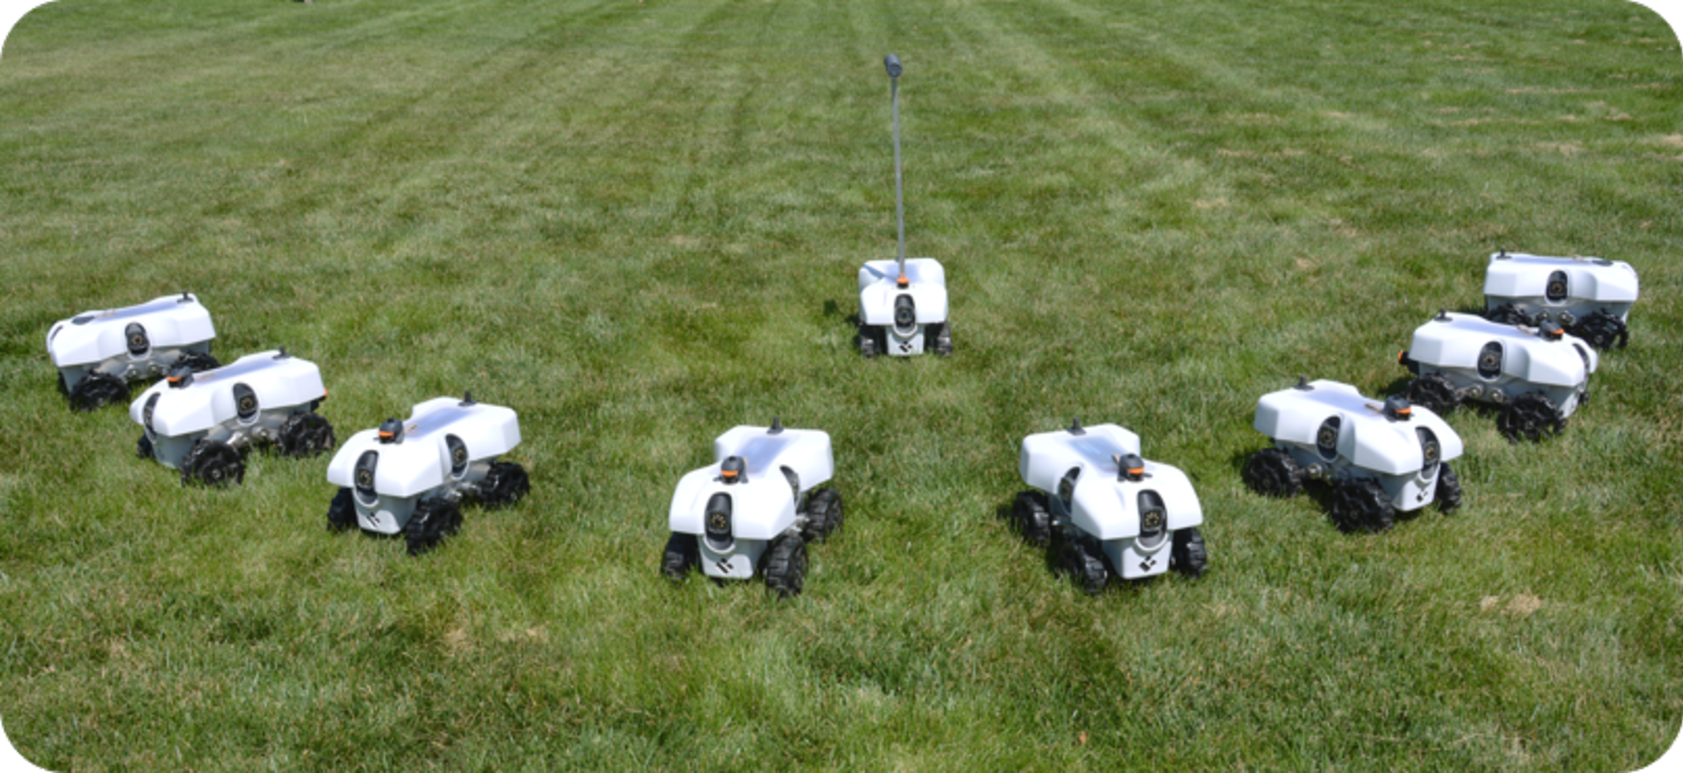
\includegraphics[width=\textwidth]{Figure S1}
\caption{The TerraSentia robots developed by Chowdhary's group at UIUC and commercialized by EarthSense inc. Agricultural robots such as these present exciting possibilities for distributed agricultural management with teams of compact, ultra-light, under-canopy robots equipped with advanced autonomy and machine learning. Such robots can fill the niche between large farm equipment and manual labor, as well as enable perennial polycultures, and closer to home,  they could also weed your garden! Advances in persistent multi-agent autonomy in harsh, changing, and uncertain environments driven by the controls community are driving such exciting possibilities of the future of agriculture.}
\label{fig:terrasentia}
\end{figure}


%\textbf{Soft robots}

\textbf{Dexterous and ubiquitous robotics for precise care} : The digital farm of the future will strive to eliminate costly inputs (chemicals, labor, energy, and knowledge) with low-cost, dexterous, and highly autonomous agricultural equipment \cite{pedersen2006agricultural}. Advances in \textit{soft} arms and grippers can enable robots that can have far better reach and dexterity around plants than robots equipped with traditional \textit{hard} industrial robotic arms. Soft arms, which are often actuated with pressurized tubes, can be far less expensive to manufacture and significantly lighter than their hard counterparts. On the other hand, soft arms can be slow to actuate and have limited payloads. To make soft robots practical, optimal feedback control techniques are necessary that work with conformal objects with very large degrees of freedom. In particular, soft arms tend to significantly deform under weight and behave quite differently when loaded with different payloads. Unlike hard arms, encoders are not sufficient to estimate the pose of the arm or the manipulator. Strain and angle sensors need to be positioned judicially to keep costs down, and image based feedback control will be necessary. The evolving Gaussian Process technique and the kernel observer techniques described in this paper could be utilized to create distributed observers for such soft systems.  

The complex interaction between closely-spaced diverse plant species in a polyculture results in both spatial and temporal dynamics as the plants grow and interact with each other. %in polyculture parameters, such as growth rate, plant phenology, and yield. 
Plant growth often exhibits hybrid dynamical systems behavior with rapid thresholded growth bursts followed by slow progression. The triggers for growth bursts are dependent on  environmental factors such as temperature, soil moisture, and sunlight reaching individual and cumulative thresholds, and complex interrelations between neighboring plants, soil chemistry, insects, and soil microbes. 

Simulating individual plant growth is an active area of research with many open questions in modeling and plant biology \cite{zhu2016plants}. Arguably, very high resolution plant growth models may not even be necessary for effective control of polycultures. Yet on the other hand, the  %TThere are many open problems in modeling 
 %Furthermore, plant growth follows sigmoidal phase transitions: even though  However, 
 existing models of plants and interactions with ecosystems \cite{Stehfest2007a,Foley1996a, Kucharik2003a,Friedl2010a, Rodrigues2010a, Nunes2013a} are not well suited for designing and managing polycultures because of the simplifying assumptions that are often made. A good balance could be struck with data driven machine learning models that have sufficient resolution for aggregate prediction over multiple spatiotemporal scales and are lightweight enough for control and decision making. With these models, predictive control strategies can be created that task teams of robots for management tasks. Furthermore, these predictive models can enable quantified mechanisms of design and planning of efficient agroecosystems.  
 Obtaining the required data to train these models and using them to create effective control techniques for managing profitable polycultures remains an exciting direction of future work where the controls community can help.
 
 The discussion in this sidebar was informed by many conversations with  crop scientists at UIUC. In particular, 
\textit{the authors wish to thank Prof. Stephen Long and Prof. Carl Bernacchi for insights on the phenotyping bottleneck and simulation of plants (\textit{crops-in-silico}), Prof. Adam Davis on inputs on the herbicide resistant weed crisis, and Prof. Sarah Lovell on sustainable agricultural production systems and perennial polycultures, as well as the members of the UIUC Center for Digital Agriculture} 

\begin{figure}[tbh]
\includegraphics[width=\textwidth]{Figure S2}
\caption{The seven layers of the forest garden. Polyculture agricultural production systems are designed ecosystems that can be more productive and sustainable than traditional monoculture systems. Managing such complex systems requires fundamental advances in robotics, spatiotemporal modeling, and control of complex biological processes, all areas where the control community can help. Figure source \cite{polyculture_fig}  see also \cite{rhodes2012feeding}.}
\label{fig:polycultures}
\end{figure}


\clearpage
\section[Feature Spaces in Machine Learning]{Sidebar: Feature Spaces in Machine Learning}\label{sb:featspace}

	
%\processdelayedfloats

\clearpage
\section[Learning Fluid Flows with Evolving Gaussian Processes]{Sidebar: Learning Fluid Flows with Evolving Gaussian Processes}\label{sb:cfd}

2nd order Partial Differential Equations (PDEs) are ubiquitous in practical science and engineering, from mechanics to transport phenomena to electromagnetics. In our view, the Navier-Stokes equations governing fluid dynamics represent most, if not all of the overall complexity of modeling these as (a) it exhibits of hybrid system behavior, e.g. elliptic-hyperbolic, and (b) the nonlinearity results in the complex spatio-temporal dynamics that are prevalent in many practical situations. The form of the NSE for compressible Newtonian fluids is expressed below, where $\mathbf u$ is the fluid velocity, $p$ is the fluid pressure, $\rho$ is the fluid density, and $\mu$ is the fluid dynamic viscosity. \cite{panton2006incompressible}

$$ \rho \left(\frac{\partial \mathbf u}{\partial t} + \mathbf u \cdot \nabla \mathbf u\right) = 
-\nabla p + \nabla \cdot \left(\mu (\nabla \mathbf u + (\nabla \mathbf u)^T)\right) + \nabla \left( - \frac{2\mu}{3}\nabla \cdot \mathbf u\right)
+ \rho \mathbf{g}$$

We demonstrate the Evolving Gaussian Processes method on CFD data of flow over a bluff body (a cylinder) over a range of Reynolds numbers from 100 to 1000 (the Reynold number is dimensionless flow rate). This deterministic, high-dimensional spatiotemporal dynamical system is well-studied in the fluid dynamics literature, both experimentally and numerically \cite{roshko1954cylinder, braza1986cylinder, rajani1986cylinder}. The conventional wisdom would be to learn a separate model over each Reynolds number, but our results show that the E-GP method is capable of learning the dynamics of all the flow patterns at once. Using the learned dynamics over weights of successive kernel models, E-GP is capable of predicting the future states of functional evolution in a recursive manner. The key advantage of E-GP is that evolution of large function spaces can be transformed into learning the evolution of a relatively smaller Hilbert space which is encoded by the kernels and the associated weight vector. Furthermore, the values of the weights and the associated linear dynamical systems provide critical insights, such as spatial-correlations through the structure of the transition matrix, local modes of dynamic evolution through invariant subspaces of the transition matrix, and eigenmodes of evolution. The latter is of significant importance to the ongoing work in Koopman operator models of spatiotemporal phenomena.

In our CFD simulation, we used a 4th-order polynomial expansion with spectral element method on the incompressible Navier-Stokes equation to generate the cylinder flow data for Re = 100, 300, 600, 800, and 1000. The spatial domain is $\left[-2,10\right]\times\left[-3,3\right]$, excluding the diameter-1 cylinder at the origin.  Neumann boundary conditions are applied to the far-field of the cylinder in the y-direction and the outlet of the flow field; and a Dirichlet boundary condition is applied to the inlet. Each data set contains at least 200 snapshots with a uniform time step of \~0.03 sec. Each snapshot contains 24,000 velocity data points for Re=100 or 95,000 velocity data points for Re=300,600,800,1000. Each data set took at least 10 hours in a high performance computer cluster to generate. Figures \ref{fig:cfd_100},\ref{fig:cfd_1000}(a-d) visualize the horizontal velocity for Re=100 and Re=1000, with red being the greatest negative velocity and blue the greatest positive velocity. The flow is unstable, periodic, and clearly nonlinear.
%The meshes are more concentrated around the cylinder and its wake in order to accurately capture the phenomenon of the flow field. The no-slip boundary condition is applied to the cylinder wall;
%In the case of Re=100, the simulated degrees of freedom (DOFs) are approximately 24,000, whereas the Re300, Re600, and Re1000 cases have 96,000 check this number, I remember is 96000, not sure!
\begin{figure*}[h]
	\centering
	\subfloat[Data from classes $A$ and $B$.]
	{
		\includegraphics[width=0.45\columnwidth]{linsep_data.pdf}
		\label{fig:lisep_data}}
	\subfloat[Linear boundary separating data.]
	{\includegraphics[width=0.45\columnwidth]{linsep_data_perceptron.pdf}
		\label{fig:lin_sep_bound}}  
	\caption{Example of linearly separable data. Any simple linear learning algorithm e.g. perceptron, finds a solution.}
	\label{fig:linsep}
	%\end{figure*}
	%\begin{figure}[tbh] %{r}{0.5\textwidth}
\end{figure*} 
\begin{figure*}[h]
	\centering
	\subfloat[Data from classes $A$ and $B$.]
	{
		\includegraphics[width=0.45\columnwidth]{figures/pres_original_data.pdf}
		\label{fig:nlisep_data}}
	\subfloat[Linear boundary fails to separate data.]
	{\includegraphics[width=0.45\columnwidth]{figures/pres_perc_original_data.pdf}
		\label{fig:nlin_sep_bound}}  
	\caption{Example of nonlinearly separable data. Perceptron fails to find a solution, and diverges.}
	\label{fig:nlinsep}
	%\end{figure*}
	%\begin{figure}[tbh] %{r}{0.5\textwidth}
\end{figure*} 
\begin{figure*}[h]
	\centering
	\subfloat[Nonlinear mapping of data.]
	{
		\includegraphics[width=0.45\columnwidth]{figures/fmapped_data.pdf}
		\label{fig:fmapped_data}}
	\subfloat[Linear boundary in new space.]
	{\includegraphics[width=0.45\columnwidth]{figures/pres_perc_fmapped_data_after.jpg}
		\label{fig:fmapped_bound}}  
	\caption{If we map the same data using a nonlinear map $\phi(x,y):= (x^2, y^2, 2xy)$, the perceptron now finds a solution
		in 3 dimensions.}
	\label{fig:fmapped}
	%\end{figure}
	%\begin{figure*}[tbh] %{r}{0.5\textwidth}
\end{figure*} 

\begin{figure*}[h] %{r}{0.5\textwidth}
	\centering
	\subfloat[Snapshot 0]{
		\includegraphics[width=0.23\textwidth]{snap100_0}		}
	\subfloat[Snapshot 10]{
		\includegraphics[width=0.23\textwidth]{snap100_10}		}
	\subfloat[Snapshot 20]{
		\includegraphics[width=0.23\textwidth]{snap100_20}		}
	\subfloat[Snapshot 30]{
		\includegraphics[width=0.23\textwidth]{snap100_30}		}\\
	\subfloat[Snapshot 0]{
		\includegraphics[width=0.23\textwidth]{snap100_c600_0}		}
	\subfloat[Snapshot 10]{
		\includegraphics[width=0.23\textwidth]{snap100_c600_10}		}
	\subfloat[Snapshot 20]{
		\includegraphics[width=0.23\textwidth]{snap100_c600_20}		}
	\subfloat[Snapshot 30]{
		\includegraphics[width=0.23\textwidth]{snap100_c600_30}		}
	
	\caption{Visualization of Fluid Flow at Re = 100, CFD (a-d), E-GP (e-h)}
	\label{fig:cfd_100}
\end{figure*}

\begin{figure*}[h] %{r}{0.5\textwidth}
	\centering
	\subfloat[Snapshot 0]{
		\includegraphics[width=0.23\textwidth]{snap1000_0}		}
	\subfloat[Snapshot 5]{
		\includegraphics[width=0.23\textwidth]{snap1000_5}		}
	\subfloat[Snapshot 10]{
		\includegraphics[width=0.23\textwidth]{snap1000_10}		}
	\subfloat[Snapshot 15]{
		\includegraphics[width=0.24\textwidth]{snap1000_15}		}\\
	\subfloat[Snapshot 0]{
		\includegraphics[width=0.24\textwidth]{snap1000_c600_0}		}
	\subfloat[Snapshot 5]{
		\includegraphics[width=0.23\textwidth]{snap1000_c600_5}		}
	\subfloat[Snapshot 10]{
		\includegraphics[width=0.23\textwidth]{snap1000_c600_10}	}
	\subfloat[Snapshot 15]{
		\includegraphics[width=0.23\textwidth]{snap1000_c600_15}	}
	\caption{Visualization of Fluid Flow at Re = 1000, CFD (a-d), E-GP (e-h)}
	\label{fig:cfd_1000}
\end{figure*}

We used the Gaussian RBF kernel $\kernel(x,y) = e^{-\|x-y\|^2/2\s^2}$ in our E-GP model, with $\s$ estimated to be 0.4. Using a budget of 600 kernel centers (see Figure \ref{fig:eigen100}-\ref{fig:eigen1000}, and note how they cluster in the most dynamic regions), we find a $600\times600$ matrix $\dualopApprox$ which accurately (Figure \ref{fig:errors}) captures the dynamics of the nonlinear system. We can use this to propagate single initial condition $\weight_{0}$ forward to make predictions, then compare the predictions to the original training data. We found total percentage errors between 3\% for Re=100 and 7-8\% for Re=1000, as can be seen in the solid lines in Figure \ref{fig:errors}. We define the total percentage errors as
$E_\tindex = \frac{\|y_\tindex-\bar y_\tindex\|_2}{\|\bar y_\tindex\|_2}$
where $\bar y_\tindex$ is the output vector for time $\tindex$ and $y_\tindex$ is the E-GP estimate at that time. Note that \emph{the size of the model has been reduced by almost two orders of magnitude} from the original CFD data. This process takes about 13 minutes in MATLAB for a 200 snapshot by 95,000 point set on an ordinary Intel i7 4.00 GHz processor.

\subsection{One Transition Matrix for Everything}\label{sec:lotr}

In order to approach the challenge of generalizing across similar spatiotemporally evolving systems, the first question we had to answer is whether we can find an $\dualopApprox$ matrix that accurately captures the dynamics of multiple similar flows. The answer to that question is \textit{yes}, using the trajectory concatenation method. Amazingly, a single model generated this way works almost as well on all five data sets as do five individual models trained on each data set separately. This is confirmed by both the total error plots (Figure \ref{fig:errors}), which show only slight increases in each of the total percentage error plots, and visual inspection of the dynamic modes displayed. This result is even more surprising in light of the fact that the rate of vortex shedding for each Reynolds number is different. By taking a Fourier transform of the time evolution of a data point located at (0.5,8), we find that for the original data sets the vortex shedding frequency is 0.448 Hz, 1.260 Hz, 1.380 Hz, 1.388, and 1.401 Hz for Re=100, 300, 600, 800, and 1000 respectively, and for the E-GP models the frequencies are 0.452 Hz, 1.21 Hz, 1.36 Hz, 1.36 Hz, and 1.36 Hz respectively.

\begin{figure*}[h] %{r}{0.5\textwidth}
	\centering
	\subfloat[\small{Universal Generalizer vs Individual Models}]{
		\includegraphics[width=0.38\textwidth]{errors}
		\label{fig:errors}		}
	\subfloat[\small{Different Models Tested on Re=800}]{
		\includegraphics[width=0.36\textwidth]{boxploterrors800}
		\label{fig:errors_boxplot}		}
	\caption{Total Percentage Errors}
\end{figure*}

\subsection{Generalizing from Learned Dynamics to Unknown Dynamics}\label{sec:generalize}

Having seen that it is possible to find a single transition in the weight space that models the dynamics systems over a range of parameters, the next challenge is to be able to model flows with parameters that the model has not been trained on. We derived an $\dualopApprox$ matrix from the Re=100, 300, 600, and 1000 data sets and tested it against the Re=800 data set. The results are below in Figure \ref{fig:errors_boxplot}. For the first 120 snapshots, the total percentage error remains under 10\%, which is satisfactory. After this, however, the total percentage error curves upwards as the slight errors in the transition matrix compound. Over 800 snapshots, we found an average total percentage error of less than 25\%. %Taking a long-range view of the error plots, we found that they curve back downward again sinusoidally at snapshot 600, 35\% error. This indicates that the source of the divergence is likely due to a slight error in the speed of the vortices. This is confirmed by Fourier analysis as above, with the generalized model producing a wake frequency of 1.427 Hz in comparison to the actual frequency of 1.388 Hz, a 2.8\% difference. This small difference explains why the model is accurate for approximately the first 10 cycles before it begins to diverge.

\subsection{Linear Dynamical Layer Analysis \& Insights}\label{sec:analysis}
Due to the spatial encoding of the weights which the linear transition model operates on, we are able to analyze the dynamics and find physical insights into the process. We demonstrate two techniques: (1) using eigendecomosition of the transition matrix to discover the eigenfunctions and invariant subspaces of system, and (2) visualizing the most significant spatial interactions in the system.


An invariant subspace of a linear operator is a subspace of the Hilbert space such that any vector in the subspace remains in the subspace under transformation by the operator. By marking which kernel centers are associated with different subspaces, we can spatially separate the space into multiple dynamic modules. The physical insight is some areas of the space are dynamically entangled with each other, and other are independent of each other. For those interested in monitoring spatiotemporally evolving systems, the number and location of the invariant subspaces determines how many and where feedback sensors ought to be for robust prediction of the weights.
\begin{figure*}[h] %{r}{0.5\textwidth}
	\centering
	\subfloat[\small{Re = 100, $\varepsilon$ = 0.005}]{
		\includegraphics[width=0.31\textwidth]{matrix100floor5e3}
		\label{fig:eigen100}	}
	\subfloat[\small{Re = 1000, $\varepsilon$ = 0.05}]{
		\includegraphics[width=0.31\textwidth]{matrix1000floor50e3}
		\label{fig:eigen1000}		}
	\subfloat[\small{All Reynolds numbers, $\varepsilon$ =0.069}]{
		\includegraphics[width=0.31\textwidth]{matrixallfloor69}
		\label{fig:eigenall}	}
	\caption{Eigenvector Heat Maps}
\end{figure*}
\begin{figure*}[h] %{r}{0.5\textwidth}
	\centering
	\subfloat[\small{Re = 100, $\varepsilon$ = 0.005}]{
		\includegraphics[width=0.30\textwidth]{subspaces100}}
	\subfloat[\small{Re = 1000, $\varepsilon$ = 0.05}]{
		\includegraphics[width=0.30\textwidth]{subspaces1000}}
	\subfloat[\small{All Reynolds numbers, $\varepsilon$ = 0.069}]{
		\includegraphics[width=0.34\textwidth]{subspacesall}}
	\caption{Invariant Subspaces}
	\label{fig:subspaces}
\end{figure*}
\begin{figure*}[h] %{r}{0.5\textwidth}
	\centering
	\subfloat[\small{Re=100}]{
		\includegraphics[width=0.31\textwidth]{Amatrix3d100.pdf}
		\label{fig:haystack100}	}
	\subfloat[\small{Re=1000}]{
		\includegraphics[width=0.31\textwidth]{Amatrix3d1000.pdf}
		\label{fig:haystack1000} }
	\subfloat[\small{Trained on all 5 data sets}]{
		\includegraphics[width=0.31\textwidth]{Amatrix3dall.pdf}
		\label{fig:haystackall}	}
	\caption{Visualization of Co-Relations in Transition Matrix}
\end{figure*}
Before doing the Jordan decomposition of $\dualopApprox$, we zero any elements smaller than some small $\varepsilon$ in order to stabilize the algorithm for matrices with many elements close to zero. Afterwards we visualize the eigenvector matrix using a \emph{logarithmic} color chart, as seen in Figures \ref{fig:eigen100},\ref{fig:eigen1000},\ref{fig:eigenall}. These plots are for models trained individually on Re=100 and Re=1000 with 300 kernels, and on all five with 600 kernels, for comparison. We see three categories of eigenvector in the rows: (1) Rows at the bottom that have exactly one non-zero elements, (2) In the middle, a couple rows with a dozen significant elements, and (3) at the top a number of rows that affect the majority of the kernel centers in the space.

Each eigenvector of (1) spans its own invariant subspace, and is depicted in magenta circles in Figure \ref{fig:subspaces}. Category (3) is one invariant subspace, depicted with black crosses. Category (2) is subsumed in Category (3). The figures show that the dynamics near/around the cylinder and in its wake are so entangled that a single sensor measurement in that area may be sufficient to estimate over that entire subspace. On the other hand, areas far from the core of dynamic excitement are their own independent, invariant subspaces, and thus must be monitored locally.

Another way to visualize the operation of the linear transition matrix is to plot lines between kernel centers that are influencing each other strongly. That is, if we draw a line center $c_j$ to $c_i$ for each of the (relatively) largest elements $a_{ij}$ of $\dualopApprox$, one can see how the system dynamics are coupled spatially (Figures \ref{fig:haystack100},\ref{fig:haystack1000},\ref{fig:haystackall}). We can also plot the magnitude of $a_ij$ in a third axis for further insight into the most dominant dynamic connection in the system.








%\begin{figure}[t]
%	\centering
%	\subfloat[\small{Gaussian}]{
%		\includegraphics[width=0.25\columnwidth]{figures/kernel_evol_gaussian.pdf}
%	}
%	\subfloat[\small{Laplacian}]{
%		\includegraphics[width=0.25\columnwidth]{figures/kernel_evol_laplacian.pdf}
%	}
%	% \\
%	\subfloat[\small{Periodic}]{
%		\includegraphics[width=0.25\columnwidth]{figures/kernel_evol_periodic.pdf}
%	}
%	% \subfloat[\small{Locally periodic}]{
%	%   \includegraphics[width=0.3\columnwidth]{figures/kernel_evol_locally_periodic.pdf}
%	%}
%	\caption{\small{One-dimensional function evolution over a fixed transition matrix $A$, 
%			initial condition $\weight_0$ and centers $\shCent$, but with different kernels $\kernel(x,y)$. 
%			Each $y$-vector at a given value of $x$ represents the output of the function, which evolves from left to right. 
%			As seen, changing the kernel creates quite different dynamic behaviors. }%behavior for the same system.}
%	}
%	\label{fig:kernel_variation}
%\end{figure}




%\begin{figure}\label{fig:linsep}
%\centering
%    \subfloat[Data from classes $A$ and $B$.]
%    {
%    \includegraphics[width=0.45\columnwidth]{figures/linsep_data.pdf}
%    \label{fig:lisep_data}}
%     \subfloat[Linear boundary separating data.]
%     {\includegraphics[width=0.45\columnwidth]{figures/linsep_data_perceptron.pdf}
%     \label{fig:lin_sep_bound}}  
%    \caption{Example of linearly separable data. Any simple linear learning algorithm e.g. perceptron, finds a solution.}
%    \label{fig:linsep}
%    %\end{figure}
%%\begin{figure}[tbh] %{r}{0.5\textwidth}
%\end{figure} 
%
%\begin{figure}
%\centering
%    \subfloat[Data from classes $A$ and $B$.]
%    {
%    \includegraphics[width=0.45\columnwidth]{figures/pres_original_data.pdf}
%    \label{fig:nlisep_data}}
%     \[Linear boundary fails to separate data.]
%     {\includegraphics[width=0.45\columnwidth]{figures/pres_perc_original_data.pdf}
%     \label{fig:nlin_sep_bound}}  
%    \caption{Example of nonlinearly separable data. Perceptron fails to find a solution, and diverges.}
%    \label{fig:nlinsep}
%    %\end{figure}
%%\begin{figure}[tbh] %{r}{0.5\textwidth}
%\end{figure} 
%
%
%\begin{figure}
%\centering
%    \subfloat[Nonlinear mapping of data.]
%    {
%    \includegraphics[width=0.45\columnwidth]{fmapped_data.pdf}
%    \label{fig:fmapped_data}}
%     \subfloat[Linear boundary in new space.]
%     {\includegraphics[width=0.45\columnwidth]{pres_perc_fmapped_data_after.jpg}
%     \label{fig:fmapped_bound}}  
%    \caption{If we map the same data using a nonlinear map $\phi(x,y):= (x^2, y^2, 2xy)$, the perceptron now finds a solution
%             in 3 dimensions.}
%    \label{fig:fmapped}
%    %\end{figure}
%%\begin{figure}[tbh] %{r}{0.5\textwidth}
%\end{figure} 
%\processdelayedfloats




\newpage
\section{Author Biography}
%Insert the author bios here.

\noindent \textbf{Joshua E. Whitman} is a PhD student at the University of Illinois in Urbana-Champaign. He received Bachelors of Science degrees in Mechanical Engineering and Mathematics from Oklahoma State University in 2015, and his Masters of Science in Mechanical Engineering from the University of Illinois in 2018. His research is centered in the fields of machine learning, controls, and autonomy, and his work focuses on developing new methods for learning, monitoring, and controlling the dynamics of complex spatiotemporally-evolving systems.

\noindent \textbf{Harshal Maske} completed his PhD in 2018 from the University of Illinois in Urbana-Champaign, he is currently a postdoc at UIUC. He received his Masters and Bachelors integrated degree in Mechanical Engineering from the Indian Institute of Technology Kharagpur, India, in 2009. After completing his masters, he worked for three years at Defense R\&D Organization (2009-2012), India and for one year at John Deere (2012-2013). His current research is grounded in the theory at the intersection of Controls and Machine learning with the aim of developing data driven models with theoretical guarantees that enable decision making and control in real-world, complex problems.

\noindent \textbf{Hassan A. Kingravi}  is a senior data scientist Eqifax, where he conducts research on machine learning and signal processing for the purposes of preventing fraud in the retail and financial sectors. He was previously with Pindrop. His research interests revolve around the interplay of control theory, signal processing, and machine learning for spatiotemporal data. He received his PhD in Electrical and Computer Engineering from the Georgia Institute of Technology in 2014 and did a postdoc at Oklahoma State University with Chowdhary's group.

\noindent \textbf{Girish Chowdhary} is an assistant professor at the University of Illinois at Urbana-Champaign and affiliated with Electrical and Computer Engineering, Agricultural and Biological Engineering, Computer Science, Aerospace Engineering, and is a member of the UIUC Coordinated Science Laboratory (CSL). He is the director of the Distributed Autonomous Systems laboratory and the Field Robotics Engineering and Science Hub (FRESH) at UIUC. He holds a PhD (2010) from Georgia Institute of Technology in Aerospace Engineering. He was a postdoc at the Laboratory for Information and Decision Systems (LIDS) of the Massachusetts Institute of Technology for about two years (2011-2013). He was an assistant professor at Oklahoma State University's Mechanical and Aerospace Engineering department (2013-2016). Prior to joining Georgia Tech, he also worked with the German Aerospace Center's (DLR's) Institute of Flight Systems for around three years (2003-2006). His undergraduate institution was the Royal Melbourne Institute of Technology in Australia. Girish's ongoing research interest is in theoretical insights and practical algorithms for adaptive autonomy with applications in field robotics. 

\end{document}
\clearpage
